% use the MIT thesis document class
\documentclass[12pt]{mitthesis}

% some packages needed for library-compliant typesetting
\usepackage{lgrind}
\usepackage{cmap}
\usepackage[T1]{fontenc}
\pagestyle{plain}

% packages Scott put into the template
\usepackage{pdfpages} % to include pdfs
\usepackage{caption} % for caption*
\usepackage{graphicx} % for figures
\usepackage{chapterbib} % for bibliographies in each chapter
\usepackage{tocloft} % for fixing table of contents
\usepackage{booktabs} % for nice tables
\usepackage{lscape} % for a landscape page (extra-wide table)

% options for controlling the table of contents typesetting
\setcounter{tocdepth}{1} % change table of contents depth
%\renewcommand{\cftchapfont}{\rmfamily} % chapters in not bold
\renewcommand{\cftchappagefont}{\rmfamily} % page in not bold

% Packages Claire needed for individual papers
\usepackage[hidelinks]{hyperref} % for links and urls
\usepackage{amsmath,amssymb} % for math
\usepackage{color,soul} % for highlighting
\usepackage{rotating,multirow} % for nice tables
\usepackage{longtable} %for multi-page tables, in aerodigestive supplement
\usepackage{float} % here for H placement parameter
\usepackage[numbers]{natbib}
\usepackage[above]{placeins} % for FloatBarrier
\usepackage{amsmath} % for pretty fraction text
\usepackage{booktabs} % for multi-line tables
%\usepackage{geometry} % for supp fig large pages
\usepackage{upgreek} % for beta in bibtex file

% Decrease space between rows in tables
\renewcommand{\arraystretch}{0.8}

\begin{document}

\title{Mining the human microbiome for clinical insight}

\author{Claire Marie Noëlle Duvallet}

\prevdegrees{B.S., Columbia University (2013)}

\department{Department of Biological Engineering}

\degree{Doctor of Philosophy in Biological Engineering}

% Valid degree months are September,
% February, or June.  The default is June.
\degreemonth{June}
\degreeyear{2019}
\thesisdate{11 January 2019}

%% By default, the thesis will be copyrighted to MIT.  If you need to copyright
%% the thesis to yourself, just specify the `vi' documentclass option.  If for
%% some reason you want to exactly specify the copyright notice text, you can
%% use the \copyrightnoticetext command.
%\copyrightnoticetext{\copyright IBM, 1990.  Do not open till Xmas.}

% If there is more than one supervisor, use the \supervisor command
% once for each.
\supervisor{Eric J. Alm}{Professor}

% This is the department committee chairman, not the thesis committee
% chairman.  You should replace this with your Department's Committee
% Chairman.
\chairman{Forest White}{Chair of Graduate Program, Department of Biological Engineering}

% Make the titlepage based on the above information.  If you need
% something special and can't use the standard form, you can specify
% the exact text of the titlepage yourself.  Put it in a titlepage
% environment and leave blank lines where you want vertical space.
% The spaces will be adjusted to fill the entire page.  The dotted
% lines for the signatures are made with the \signature command.
\maketitle

% The abstractpage environment sets up everything on the page except
% the text itself.  The title and other header material are put at the
% top of the page, and the supervisors are listed at the bottom.  A
% new page is begun both before and after.  Of course, an abstract may
% be more than one page itself.  If you need more control over the
% format of the page, you can use the abstract environment, which puts
% the word "Abstract" at the beginning and single spaces its text.

% You can either \input (*not* \include) your abstract file, or you can put
% the text of the abstract directly between the \begin{abstractpage} and
% \end{abstractpage} commands.
\cleardoublepage
\setcounter{savepage}{\thepage}
\begin{abstractpage}
%% The text of your abstract and nothing else (other than comments) goes here.
%% It will be single-spaced and the rest of the text that is supposed to go on
%% the abstract page will be generated by the abstractpage environment.

The human microbiome is essential for health and has been implicated in many diseases.
DNA sequencing has enabled the detailed characterization of these human-associated microbial communities, leading to a rapid expansion in studies investigating the human microbiome.
%However, extracting clinically-relevant associations from microbiome datasets remains challenging because of the high dimensional nature of the data and variability across studies.
In this thesis, I describe three projects which overcome various data analysis challenges to extract useful clinical insights from microbiome data.
In the first project, I present an analysis of lung, stomach, and oropharyngeal microbiomes.
I leverage data collected from multiple sites per patient to identify aspiration-associated changes in the relationships between aerodigestive communities, discovering new properties of the aerodigestive microbiome and suggesting new approaches for treatment.
%These changes suggest new approaches for developing diagnostics and treatments for aspiration-related respiratory complications.
%I leverage data collected from multiple sites per patient to find aspiration-associated changes in the relationships between aerodigestive communities which suggests new targets for treatment and diagnosis.
In the second project, I perform a meta-analysis of case-control gut microbiome datasets with standard data processing and analysis methods.
I find consistent patterns characterizing disease-associated microbiome changes and a set of shared associations which could inform clinical treatment and therapeutic development approaches for many different microbiome-mediate diseases.
In the third project, I describe a framework for rational donor selection in fecal microbiota transplant clinical trials.
In this framework, knowledge derived from clinical and basic science research is used to inform which donor is selected for fecal transplants, increasing the likelihood of successful trials.
Together, these projects demonstrate a variety of approaches to mine the human microbiome for clinically-relevant insights and suggests multiple avenues forward for translating findings from microbiome data analyses into clinical impact.

\end{abstractpage}

\cleardoublepage

\section*{Acknowledgments}

Mentors:
Rafa - will always be a friend of the lab
Jim
Deb
Ilana - for being the mentor I didn't know I needed

Thomas - being my first introduction to computational work with patience and enthusiasm, enabling me to find my passion here
Mariana - drive and ability to make impossible things actually happen was an inspiration, expanded the scope of what a PhD student could do
Scott - being a role model, mentor, collaborator, and now close friend. Hope you remain all four forever. Also for encouraging me to start doing diversity and REFS
Sean Gibbons - modeling pure interest in science for the sake of science, encouraging me and being patient when I thought it was all fake, modeling success and being a joy to work with

Peers:
Nathaniel
Diversity co-conspirators: Scott and Manu, Bevin, and now my GSC crew for revitalizing me in the work (Nas, Josue, Danielle, German, Halston, and Bianca)

Funding:
NDSEG
Siebel

Friends, family, and frisbee
Carolyn and Megan
Andee and Shelby
Janyne for keeping me adventuring
sMITe
Felix (for GTD, 20% rule, and inspiration to version control everything)
ET (for putting us to shame by having a job and real life)
Parents (for supporting me, recognizing my passions better than I do, and listening to me talk about poop over many dinners)

\pagestyle{plain}
\include{contents}

% include each tex file
%% This is an example first chapter.  You should put chapter/appendix that you
%% write into a separate file, and add a line \include{yourfilename} to
%% main.tex, where `yourfilename.tex' is the name of the chapter/appendix file.
%% You can process specific files by typing their names in at the
%% \files=
%% prompt when you run the file main.tex through LaTeX.

\chapter{Introduction}

\section{The human microbiome in health and disease}

The microbes that live in and on our bodies make up the human microbiome, are essential for health, and have been implicated in many diseases.
Almost all human body sites are colonized by microbes, ranging from the gut, the largest human-associated microbial community, to the lungs, which were for many years considered sterile \cite{sender-2016-bhratio,beck-2012-lungmicrobiome}.
These microbial communities perform essential functions for health, including fighting off and preventing infections, regulating host metabolism and interacting with the immune system, and metabolizing xenobiotics or other compounds which are indigestible by the host.
Additionally, perturbations in human microbiomes have been implicated in many diseases, including inflammatory, metabolic, neurological, and respiratory conditions \cite{beck-2012-lungmicrobiome,ibd-papa,ridaura-2013-obfmt,hsiao-2013-autism}.

The potential for microbiome-based therapies to improve human health and address a broad range of diseases has led to a recent expansion of research and clinical studies in this field.
Much of the emerging research has been driven in part by the increasing accessibility of DNA sequencing technology, which can provide a detailed view of the bacteria in these communities without the need for time-consuming and difficult culturing experiments \cite{hmp-2012}.
However, identifying clinically-relevant associations from microbiome studies remains challenging \cite{knights-2011-predictivevalue}.
Microbiome datasets are high-dimensional, with hundreds to thousands of bacterial species measured in usually only tens to hundreds of patient samples.
Microbial communities are also highly variable across people, making it more difficult to identify individual bacterial biomarkers that can consistently distinguish health and disease across many different patients.
Finally, microbiome datasets provide a window into associations but not causal relationships, and researchers must perform follow-up mechanistic studies or clinical trials to confirm the clinical relevance of any identified associations.
In this thesis, I present unique analyses of microbiome data which overcome some of these challenges and which illustrate a variety of approaches for extracting useful clinical insights from mining microbiome data.
Together, the following chapters aim to move findings from the individual microbiome data analyses beyond statistical significance and toward clinical meaningfulness.

\section{Multi-site sampling to identify clinical associations in the aerodigestive microbiome}

In Chapter \ref{chap:aspiration}, I leverage simultaneous sampling within patients to identify clinically-relevant aerodigestive microbiome characteristics that distinguish patients with swallowing dysfunction from those with normal swallow.
The current gold standard to diagnose aspiration resulting from impaired swallow function involves imaging a patient as they ingest different quantities and consistencies of contrast material \cite{cook-1999-dysphagia}, but identifying lung microbial biomarkers could provide a useful non-radioactive alternative to this diagnosis.
Additionally, patients with impaired swallow function are at higher risk for respiratory infections, but the extent to which the lung microbiome is perturbed by aspiration and thus potentially involved in mediating this risk is unknown \cite{cook-1999-dysphagia,thomson-2016-asppneumo}.
Finally, clinical interventions to treat respiratory symptoms in patients with impaired swallow focus on preventing material transfer from the stomach into the lungs, for example via anti-reflux medication or fundoplication surgery \cite{goldin-2006-fundo,lee-2008-fundo}.
However, the clinical utility of these interventions in pediatric populations is not fully established, and the extent to which the gastric vs. mouth microbiome mediates respiratory complications is not known.

In this study, I analyzed a set of aerodigestive microbiome samples collected from over 200 patients at Boston Children's Hospital.
I first show that lung and stomach microbiomes are highly variable across people and driven primarily by person rather than body site, complicating the search for a reliable microbial biomarker of aspiration across patients.
I overcome this challenge by leveraging the fact that we have multiple samples per patient, comparing instead the within-patient \textit{relationships} between microbial communities in the aerodigestive tract of patients with and without aspiration.
Using this approach, I show that aspiration shifts lung microbial communities toward the oropharyngeal but not the stomach microbiome, suggesting that the mouth is likely an important source of lung microbiome changes in these patients.
Thus, approaches for treating aspiration-related respiratory symptoms should target microbial transfer from the mouth into the lungs in addition to focusing on the gastric-lung axis, as most current interventions do.
This study also illustrates the power of multi-site within-patient sampling to overcome variability across people to identify clinically meaningful microbiome-based biomarkers.

\section{Re-analyzing datasets to find consistent patterns of associations between the gut microbiome and disease}

In Chapter \ref{chap:meta-analysis}, I perform a meta-analysis of 28 case-control gut microbiome studies across 10 diseases to synthesize findings across studies and identify generalizable associations.
Although the human gut microbiome has been extensively studied in many diseases, there is little consensus on which disease associations are consistent across patient cohorts.
In other fields like medicine or psychology, consensus is usually achieved through meta-analyses of published literature \cite{glass-1976}.
However, comparing published results across microbiome studies is not straightforward.
The field lacks standard data processing and analysis methods, making many reported results impossible or inappropriate to compare directly between studies.
For example, different studies often use incompatible bioinformatics or statistical methods: they may compare bacteria at different taxonomic levels and use different bioinformatics workflows, and they may identify significant associations through univariate statistical tests or machine learning models, results from which can not be readily compared \cite{edd-singh,crc-baxter,crc-zeller,ob-zupancic}.
Additionally, studies led by clinicians often ask very different questions of the data than studies led by microbial ecologists, and so the reported results are not necessarily representative of the comprehensive information contained in the full dataset \cite{asd-son,ra-scher,nash-wong}.
This issue is especially relevant in this field, where non-invasive sample collection and open-source bioinformatics software suites have made microbiome research accessible to a broad range of scientists and clinicians.

In this chapter, I perform a meta-analysis of gut microbiome studies which overcomes many of these challenges by reprocessing and reanalyzing raw data with standard methods.
Even though specific bacterial associations vary across studies of the same disease, I identify patterns of general microbiome shifts which are consistent  and which suggest different approaches for developing microbiome-based therapeutics.
When looking across multiple diseases, I find a set of bacteria which are non-specifically associated with health and disease, perhaps forming a shared or core response to general health and disease status.
These results highlight the importance of contextualizing results from individual studies within the existing body of work, and also hints at the possibility of developing broadly beneficial targeted probiotic and antibiotic therapies.

\section{Enabling more powerful meta-analyses by developing a batch correction method for microbiome data}

Motivated and enabled by the work presented in Chapter \ref{chap:meta-analysis}, I present a method to correct for batch effects in case-control microbiome studies in Chapter \ref{chap:perc-norm}.
Traditionally, meta-analyses compile published p-values and effect sizes and determine their consistency, significance, and magnitude across studies to glean an overall understanding of true effects \cite{glass-1976}.
However, this is challenging to do in the microbiome research field for reasons described above and in Chapter \ref{chap:meta-analysis}.
A more powerful way to synthesize findings across studies is to combine the raw data and re-perform analyses on this expanded sample size.
However, analyzing raw data combined from multiple studies is not appropriate without first correcting for batch effects.
In microbiome data, batch effects result from biological and technical variation between studies and although statistical methods to correct for these have been developed for other `omics data types, few are applicable for microbiome data \cite{gibbons-2018}.

In this chapter, we describe a method to correct for batch effects in microbiome data.
Briefly, the method converts the abundances of taxa in case samples to percentiles of their respective distributions in the control samples within each study, in essence considering control samples as the null.
Assuming that control patients should represent biologically similar groups, this allows for pooling of percentile-normalized data across studies.
We show that this non-parametric method successfully removes batch effects in case-control studies, enabling more powerful analyses on combined microbiome data and reducing the number of false positives from individual analyses.
My main contributions to this joint work were processing the datasets used to develop and test the method and implementing the method into a popular microbiome software suite, QIIME 2 \cite{qiime2}, expanding its reach and accessibility.

\section{Translating microbiome research through rationally designed fecal microbiota transplant clinical trials}

In Chapter \ref{chap:donor-selection}, I present a framework for rationally selecting donors in fecal microbiota transplant (FMT) clinical trials.
In recurrent \textit{Clostridium difficile} infection (rCDI), FMTs have proven themselves as a remarkably effective clinical treatment, generating excitement about the clinical potential of FMTs in other diseases \cite{quraishi-2017-rcdifmt,bafeta-2017-fmt}.
Clinical trials in non-rCDI diseases can be used to identify promising conditions in which the microbiome may have a causal role to play.
However, although there is little donor-dependent variability in FMT efficacy in rCDI, it is becoming apparent that in many other non-rCDI conditions, donor heterogeneity likely plays a role in patient response \cite{moayyedi-2015,olesen-2018-superstool}.
Thus, as FMT trials expand to new indications, many trials may fail not because the indication was not amenable to improvement by FMT but rather because an ineffective donor was chosen.
As a consequence, excitement and support for FMT research will be dampened, slowing progress toward finding clinical applications of microbiome-based therapies.

In this chapter, we present an approach for selecting donors in FMT trials to increase the likelihood that these trials will succeed.
In our proposed framework, a clinician applies her existing knowledge and hypotheses for how her indication of interest is being mediated by the microbiome to drive the donor selection process.
We present four types of disease models to describe underlying processes mediating microbiome-related diseases: acute dysbiosis, mediation by individual taxa, missing or overactive community function, and complex host-microbiome interactions.
We suggest associated donor selection strategies for each of these disease models, and provide case studies illustrating the process of selecting donors rationally.
Finally, I perform a power simulation which finds that most FMT trials are unlikely to be powered enough to identify the key donor bacteria mediating patient responses to FMT.
Thus, to successfully make discoveries from completed trials, clinicians should perform hypothesis-driven retrospective analyses and plan for these during the clinical trial design process, for example by collecting paired donor and patient and/or longitudinal samples.
The framework that we present encourages clinicians to leverage their clinical experience, existing microbiome research and published datasets, and the increasing availability of screened donor stools to more efficiently translate microbiome research into clinical impact.
It also suggests approaches for improving retrospective analyses of the microbiome data generated during these clinical trials.

\section{Mining the microbiome and metabolome of residential sewage for community-level public health surveillance}

In Chapter \ref{chap:24hr}, I present preliminary work analyzing untargeted metabolomics and microbiome data of residential sewage for human health and activity markers with public health relevance.
Wastewater epidemiology has long been proposed for many applications in population health, but has so far found only limited success in polio surveillance \cite{polio} and illicit drug consumption monitoring \cite{Subedi2014,Ort2014}.
Standard wastewater epidemiology methods sample sewage at the wastewater treatment plant and perform targeted analyses to measure individual metabolites or viruses of interest.
Sampling at the treatment plant can capture information about large urban populations, but does not provide spatially resolved information about individual communities within the city.
This makes current wastewater epidemiology methods inappropriate for many public health applications, since a major goal of public health activities is to reduce disparities between populations by tailoring interventions to specific high-risk groups \cite{Ramaswami2018,Weeramanthri2018,Khoury2016}.
Implementing wastewater epidemiology within communities could be used to evaluate the impact of neighborhood-level public health campaigns or policy changes.
As one example, although it would take many years to measure the impact of a citywide sugar tax on obesity rates, biomarkers of human sugar consumption should quickly decrease upon the implementation of the tax in neighborhoods where it is expected to have a large impact.

In this chapter, we present a platform to implement wastewater epidemiology within cities that mines the metabolome and microbiome of residential sewage to find biomarkers with potential public health relevance.
This project is the culmination of a large collaboration between computational biologists, urban designers, engineers, city workers, and public health officials, and it is presented in its entirety in Chapter \ref{chap:24hr}.
My contribution to this work was identifying and confirming many human biomarkers in the untargeted metabolomics data.
By comparing the masses and fragmentation spectra of our metabolite features with databases and published work, I identified over 20 glucuronide compounds which are direct markers of human excretion and were abundant in our residential sewage samples but rarely detected at downstream sites.
In collaboration with our mass spectrometry specialist, we confirmed multiple urinary and fecal metabolites and showed that these reflected expected human activity patterns over the course of a 24-hour hourly sampling.
Further putative matches between our metabolomics features and a large database of human metabolites \cite{hmdb} suggests that this work could be extended to identify many different types of biomarkers reflecting human health, diet, and lifestyle.

\begin{singlespace}
\bibliography{chap1}
\bibliographystyle{unsrt}
\end{singlespace}

%% This is an example first chapter.  You should put chapter/appendix that you
%% write into a separate file, and add a line \include{yourfilename} to
%% main.tex, where `yourfilename.tex' is the name of the chapter/appendix file.
%% You can process specific files by typing their names in at the
%% \files=
%% prompt when you run the file main.tex through LaTeX.

\graphicspath{{aspiration/figures/}}

\chapter{Multi-site sampling reveals altered relationships in aerodigestive microbiomes of children with swallowing dysfunction}\label{chap:aspiration}

Claire Duvallet, Kara Larson, Scott Snapper, Sonia Iosim, Ann Lee, Katherine Freer, Kara May, Eric J Alm, and Rachel Rosen.

\bigskip
\bigskip
\noindent
The contents of this chapter have been submitted for publication as: ``Aerodigestive sampling reveals altered microbial exchange between lung, oropharyngeal, and gastric microbiomes in children with impaired swallow function,'' in review as of December 2018.

\bigskip
\bigskip
\noindent
The tables and figures are at the end of the Chapter. The Supplementary Information is in Appendix \ref{app:aspiration}.

\clearpage
% % Double-spaced
%\usepackage{setspace}
%\onehalfspacing

\section*{Abstract}

\subsection*{Background}

Children with oropharyngeal dysphagia have impaired airway protection mechanisms and are at higher risk for pneumonia and other pulmonary complications.
Aspiration of gastric contents is often implicated as a cause for these pulmonary complications, despite being supported by little evidence.
The goal of this study is to determine the relative contribution of oropharyngeal and gastric microbial communities to perturbations in the lung microbiome of children with and without oropharyngeal dysphagia and aspiration.

\subsection*{Methods}

We conducted a prospective cohort study of 222 patients consecutively recruited from a tertiary aerodigestive center undergoing simultaneous esophagogastroduodenoscopy and flexible bronchoscopy.
Bronchoalveolar lavage, gastric and oropharyngeal samples were collected and 16S sequencing was performed.
A subset of patients also underwent video fluoroscopic swallow studies to assess swallow function and were categorized as aspiration/no aspiration.
Microbial communities across the aerodigestive tract were compared in patients with and without aspiration by calculating within-patient beta diversities and quantifying microbial exchange across sites.

\subsection*{Results}

Within all patients, lung, oropharyngeal and gastric microbiomes overlap.
The degree of similarity is the lowest between the oropharynx and lungs (median Jensen-Shannon distance (JSD) $=$ 0.90), and as high between the stomach and lungs as between the oropharynx and stomach (median JSD $=$ 0.55 and 0.56, respectively; p $=$ 0.6).
Unlike the oropharyngeal microbiome, lung and gastric communities are highly variable across people and driven primarily by person rather than body site.
In patients with aspiration, the lung microbiome more closely resembles oropharyngeal rather than gastric communities and there is greater prevalence of microbial exchange between the lung and oropharynx than between gastric and lung sites (p $=$ 0.04 and 3x10$^{-5}$, respectively).

\subsection*{Conclusions}

The gastric and lung microbiomes display significant overlap in patients with intact airway protective mechanisms while the lung and oropharynx remain distinct.
In patients with impaired swallow function and aspiration, the lung microbiome shifts towards oropharyngeal rather than gastric communities.
This finding may explain why antireflux surgeries fail to show benefit in pediatric pulmonary outcomes.

\newpage
\section{Introduction}

The economic and social impact of oropharyngeal dysfunction and aspiration is well known in the adult stroke population; adults with oropharyngeal dysfunction are at greater risk of pneumonia than those without \cite{holas1994aspcomplications}.
Little is known about aspiration-related lung disease in children, though recent studies suggest that up to 10\% of all pneumonia hospitalizations in pediatrics are related to aspiration \cite{thomson2016asppneumo}.
Clinicians often assume these pneumonias result from the aspiration of refluxed gastric contents and frequently treat these children with antireflux surgery, fundoplication.
Despite this common surgical practice, there are no pediatric studies which conclusively show improved pulmonary outcomes after fundoplication, suggesting that the respiratory symptoms seen in aspirating patients may not be related to aspiration of gastric contents \cite{barnhart2013fundo,lee2008fundo,goldin2006fundo,yeh2016,srivastava2009fundo}.
An alternative hypothesis is that aspiration-related respiratory symptoms may result from aspirated oropharyngeal contents.
To test this hypothesis, we determined the microbial signatures of the lungs, stomach, and oropharynx in children with and without oropharyngeal dysphagia (i.e. with and without impaired airway protective mechanisms) to determine the relative contributions of the oropharyngeal and gastric microbiomes to the lung microbiome.

Previous studies have shown that the mouth, upper respiratory tract, and lung microbiota contain similar microbes, and that upstream oral communities seed downstream sites (e.g. lungs and stomach) \cite{Bassis2015source,Charlson2011topographical,rosen2015ppi}.
However, there is little consensus on whether there exists a distinct or "core" lung microbiome that is consistent across people \cite{Charlson2011topographical,venkataraman-2015-dispersal,segal-2013-pneumotypes,erbDownward-2011-COPD}.
Most studies, however, agree that the lung microbial communities share taxa with the oral microbiome, but that there are some bacteria present in lung communities whose abundances cannot be traced solely to the mouth \cite{Bassis2015source,Charlson2011topographical,morris-2013-healthsmokers,segal-2013-pneumotypes}.

While the importance of oropharyngeal flora in seeding the lungs has been heavily studied in ICU settings \cite{tantipong2008decontamination,koeman2006decontamination,hu2010pseudo}, the role of oropharyngeal-lung flora exchange in otherwise heathy children with isolated swallowing dysfunction is unknown.
Furthermore, studies investigating the relationships between microbial communities across the aerodigestive tract have not examined how microbes exchange between the stomach and lungs, and how this exchange relates to clinical factors such as aspiration and gastroesophageal reflux.

If the lung microbiome of aspirating patients exhibits more exchange with the oropharynx than the stomach, this could provide evidence for why anti-reflux surgery is not helpful in patients with aspiration-related respiratory symptoms.
Furthermore, a shift in the lung microbial communities toward an oropharyngeal population could not only result in overt pneumonia but may also have more subtle, pro-inflammatory effects \cite{segal-2016-inflammation}.
Finally, if there is a unique aerodigestive microbial signature in aspirating patients, microbial profiling may be helpful as a diagnostic tool for oropharyngeal dysphagia.

\section{Methods}

\subsection{Patient cohort and sample collection}

We conducted a prospective cross sectional cohort study of children ages 1--18 undergoing bronchoscopy and esophagogastroduodenoscopy (EGD) for the evaluation of chronic cough.
Patients with gastrostomy or nasogastric tubes, a history of gastrointestinal surgery, or antibiotics within 4 weeks of sample acquisition were excluded.
The study was approved by the Boston Children's Hospital Institutional Review Board and informed consent was obtained from all patients/parents.

We first performed brushing of the posterior tongue to obtain oropharyngeal samples, placing the brush in TE buffer at -80C.
Second, the bronchoscopy and bronchoalveolar lavage (BAL) was performed through an endotracheal tube in distal airways of the right middle lung or the most visually inflamed lung.
Finally, gastric sampling was performed during the EGD.
The endoscope was advanced, without suctioning, immediately into the stomach where the gastric fluid was suctioned into a sterile leukitrap.
A minimum of 1 cc of gastric and lung fluid were collected and transferred to -80C.
Each patient had a triad of samples collected: oropharynx, gastric fluid, and BAL (Tables \ref{tab1} and \ref{tab2}) \cite{rosen2015ppi}.

\subsection{Multichannel intraluminal impedance with pH (pH-MII)}

A subset of patients had pH-MII testing at the discretion of the patient's primary gastroenterologist.
Acid reflux episodes were defined as episodes detected by the impedance (MII) sensors with associated drop in pH to $<$ 4; non-acid episodes did not have the associated drop.
The percentage of time that reflux was in the proximal/distal esophagus was calculated by dividing the sum of the bolus clearance times in the proximal/distal esophagus by the total study duration.
The percentage of full column reflux events was defined as the percentage of the total reflux events that reached the proximal two impedance sensors (i.e., the proximal most impedance channel) \cite{rosen2004impedance}.

\subsection{Oropharyngeal dysphagia assessment}

A subset of the patients included in this study had a videofluoroscopic swallow study (VFSS) to asses swallow function and were divided into two groups (normal swallow function and aspiration/penetration).
Because patients with penetration on VFSS have similar pulmonary symptoms and respond similarly to thickening as patients that aspirate, we included patients with aspiration and penetration in one group.

\subsection{Sample processing and sequencing}

Oropharyngeal swabs, BAL, and gastric fluid samples suspended in Tris-Saline buffer were centrifuged for 3 minutes at 10,000 rcf prior to DNA isolation.
DNA was extracted from the sample pellet with the Qiagen DNeasy PowerSoil Kit as described by the manufacturer, with the following modifications: protein precipitation in one step using 100 $\mu$L of each C2 and C3 solutions, and column centrifugation at 10,000 rcf for 10 minutes.
Sequencing was performed in two batches at the Broad Institute.
Patients with multiple samples had all of their respective samples sequenced in the same batch.

\subsection{Microbiome data processing and analysis}

Paired end reads were merged using USEARCH \texttt{-fastq\_mergepairs} and truncated to 200 bp.
Reads with more than 2 expected errors were discarded.
Operational taxonomic units (OTUs) were clustered at 99\% similarity and assigned taxonomy using the RDP classifier (c $=$ 0.5) \cite{wang2007rdp}.
All quality filtering and OTU calling steps were performed with an in-house pipeline \\ (https://github.com/thomasgurry/amplicon\_sequencing\_pipeline).

Beta diversity was calculated with the Jensen-Shannon distance (JSD).
Only samples which were sequenced in the same batch were considered in cross-patient comparisons.
Differences in overall community structure across sites was assessed using the PERMANOVA test as implemented in scikit-bio v 0.4.2 (\texttt{skbio.stats.distance.permanova}).

To define exchanged OTUs, we used data from patients with all three sites sequenced.
For each OTU, we calculated the Spearman partial correlation ($\frac{r_{xy} - r_{xz}r_{zy})}{\sqrt{(1 - r_{xz}^2)(1 - r_{zy}^2)}}$) between its non-zero abundances in two sites, partialled on the third site (Scipy v 0.19.0 \texttt{stats.spearmanr}).
P-values for each OTU were calculated as the percentage of null correlations larger than the observed correlation after shuffling abundances 2000 times.
Only OTUs present in two sites in at least 10 patients were considered.
OTUs with FDR-corrected q-value $<$ 0.1 were defined as ``exchanged'' (\texttt{sandbox.stats.multicomp.multipletests} with \texttt{method=`fdr\_bh'}).
To determine the statistical significance of the number of exchanged OTUs, we shuffled the patient IDs for each OTU in each site and re-defined ``null'' exchanged OTUs as described above.

We used five-fold cross-validation and Random Forest classifiers (scikit-learn v 0.18.1 \newline \texttt{ensemble.RandomForestClassifier} with n\_estimators=1000) for all supervised machine learning analyses.
Areas under the ROC curve (AUCs) were calculated based on the predictions on each fold's test set (mean values across folds is reported) and Fisher p-values were calculated from all test set predictions.
The aspiration/non-aspiration classifiers varied different train/test splits, so we report the mean results across 100 repetitions.

\subsection{Availability of data and materials}
Code to reproduce the analyses presented here are available at www.github.com/cduvallet/aspiration-analysis-public.
The 16S sequencing data used in this study will be made available in the SRA repository at accession number SRP141148 upon publication and clinical metadata are available upon request from the corresponding author.

\section{Results}

Two hundred and twenty two patients were included in the analysis (Tables \ref{tab1} and \ref{tab2}).
The mean age of the patients was 7.1 $\pm$ 5.4 years.
One hundred out of 222 patients were taking proton pump inhibitors at the time of sampling.
One hundred and four patients had a videoflouroscopic swallow study of which 47 (45\%) had evidence of aspiration or penetration and 57 (55\%) had normal swallow function.
Thirty one patients had pH-MII testing for gastroesophageal reflux at the time of sample collection.

\subsection{Aerodigestive microbiome across people}

%To \textbf{characterize the baseline composition of aerodigestive communities}, we examined patients who had all three sites (oropharyngeal swab, lung, and gastric fluid) sequenced (Table \ref{tab:intra_samples}).
%Similarly to the adult aerodigestive microbiome,
At the genus level, pediatric aerodigestive communities share many predominant members, including \textit{Streptococcus}, \textit{Prevotella}, \textit{Haemophilus}, \textit{Veillonella}, and \textit{Neisseria} (Figure \ref{fig1}).
Despite genus-level similarities, OTU-level aerodigestive communities are distinct and highly variable across people.
The overall community composition was significantly different between sites (PERMANOVA on JSD, p $<$ 0.001, Figure \ref{fig2}B).
Furthermore, lung communities were very different across people (median lung-lung JSD $=$ 0.88) while oropharyngeal communities tended to be more similar (median oropharyngeal-oropharyngeal JSD $=$ 0.59, Figure \ref{fig2}A).

%These findings point to a lack of an OTU-level ``core'' lung microbiome, and complicate the search for reliable non-pathogenic microbial biomarkers in the lung microbiome, since most patients will have few lung OTUs in common with other patients.

%Proteobacteria and Firmicutes were the most abundant phyla in the aerodigestive microbiome, comprising more than half of the relative abundance in all three sites.
%\textit{Streptococcus} and \textit{Haemophilus} were among the top three most abundant genera in all three sites.
%\textit{Prevotella} was the most abundant genus (21\% average abundance) in the oropharyngeal samples and among the top ten most abundant genera in the other sites (9\% and 3\% average abundance in gastric fluid and lungs, respectively).

%\textbf{Despite similar genus-level taxonomic profiles, aerodigestive sites are distinct and variable across people.}


\subsection{Aerodigestive microbiome within people}

We compared aerodigestive communities within patients who had multiple sites sequenced (Table \ref{tab2}, Figure \ref{fig3}).
Oropharyngeal and gastric fluid communities are similar within patients (median JSD $=$ 0.56), reflecting that the mouth seeds the gastric microbiome \cite{Bassis2015source,Charlson2011topographical}.
The majority of patients had very different lung and oropharyngeal communities (median JSD $=$ 0.90), and these differences were significantly higher than either the lung-gastric fluid or gastric fluid-oropharyngeal beta diversities (p $< 1 \times 10^{-8}$, Figure \ref{fig3}A).
Surprisingly, lung and stomach communities were as similar to each other as stomach and oropharyngeal communities (median JSD $=$ 0.55 versus median JSD $=$ 0.56, respectively, p $=$ 0.6).
%One possible explanation for these similar gastric and lung communities is that they are both being seeded by the oropharynx, resulting in similar compositional profiles \cite{Bassis2015source,venkataraman-2015-dispersal}.
%Alternatively, as our data has previously suggested, the lungs and stomach may directly exchange bacteria through microaspiration of gastric contents or coughing and subsequent swallowing \cite{rosen2011culture}.
%Finally, both the lungs and stomach have low biomass and harsh selective pressures, which may lead to similar community taxonomic profiles without necessarily requiring direct exchange of individual bacteria \cite{Bassis2015source,venkataraman-2015-dispersal,Dickson2014}.

To identify specific microbes exchanging between sites, we reasoned that an actively exchanging microbe's abundances in two sites should be correlated across patients (Supplementary Figure A-1 and Methods).
We identified 12 OTUs exchanged between lung and oropharyngeal, 74 between gastric fluid and lung, and 118 between oropharyngeal and gastric fluid communities.
These results were statistically significant: we found a maximum of 2 exchanged OTUs between sites in our null analysis.
The low number of directly exchanged OTUs between the oropharynx and lungs supports the finding that these sites are more distinct than others in the aerodigestive tract.
The lungs and stomach exchange fewer OTUs than the oropharynx and stomach even though they have comparable intra-patient similarities, suggesting that factors other than specific bacterial exchange contributes to the similarity between lungs and stomachs within patients.

Random Forest classifiers trained to distinguish between sites (ensuring that samples from the same patient were in the same train/test set) were able to identify a generalizable oropharyngeal microbial signature that distinguishes the oropharynx from other sites across people (AUC $=$ 0.95 for both gastric fluid and lung comparisons, Figure \ref{fig3}B).
Surprisingly, when we compared within-patient similarities across sites to across-patient similarites for the same sites, we found that lung and stomach communities within patients were more similar than lungs across patients and than stomachs across patients (Table \ref{tab3}, p $< 1 \times 10^{-8}$).
Thus, while there exists a ``core'' oropharyngeal microbiome across people, lung and gastric communities are more variable and driven primarily by the person rather than body site.
These results challenge the prevailing hypothesis that human-associated microbial communities are primarily driven by body habitat and instead suggest that patient-specific relationships may be equally, if not more, important in determining community structure in the aerodigestive microbiome \cite{costello2009bodysites,huttenhower2012hmp,lozupone2013bodysites}.

\FloatBarrier

\subsection{Aspiration modulates the relationship between lung and oropharyngeal microbiomes but not the lung and stomach}

Next, we investigated the impact of oropharyngeal dysphagia and aspiration on the relationships between aerodigestive microbiomes.
Aspirators had significantly more similar lung and oropharyngeal communities than non-aspirators (Figure \ref{fig4}A, p $=$ 0.04) and were much more likely to have the pre-defined oropharyngeal-lung microbes in both their oropharynx and lungs than non-aspirators (p $= 2 \times 10^{-5}$) (Figure \ref{fig4}B).
Lung-oropharynx exchanged OTUs co-occurred in a median of 42\% of aspirators' lung and oropharyngeal communities but only 20\% of non-aspirators'.
Aspirators were not more likely to have stomach-lung microbes present in both the lungs and gastric fluid than non-aspirators (Figure \ref{fig4}B, p $>$ 0.5), and lung and gastric communities of aspirating patients were not necessarily more similar to each other than those of non-aspirating patients (Figure \ref{fig4}A, p $=$ 0.5).

To identify potential microbial biomarkers of aspiration, we looked at the exchanged OTUs which were most frequently present in the lung and oropharyngeal communities of aspirators relative to non-aspirators.
In the oropharyngeal-lung exchanged OTUs, these were an unknown OTU in the \textit{Flavobacteriaceae} family, OTUs in the \textit{Fusobacterium}, \textit{Rothia}, \textit{Veillonella} genera, and an unknown OTU in the \textit{Prevotellaceae} family, among others (Table \ref{tab4}, gastric-lung OTUs in Supplementary Table A-1).

We used Random Forest classifiers trained on the presence of exchanged OTUs in different sites to test their potential as biomarkers.
The concordant presence or absence of exchanged OTUs in the two sites improved classifiers based on the oropharyngeal-lung OTUs but not the ones based on the lung-gastric OTUs, relative to classifiers based on the presence of the exchanged OTUs in either site alone (Table \ref{tab5}).
Using Random Forest classifiers trained on the entire microbiomes, we found that combining the oropharynx and lung communities resulted in a better classifier than either community alone (Table \ref{tab6}).
Surprisingly, the classifiers trained on oropharyngeal and gastric communities performed well, despite our expectation that aspiration-induced changes in the microbiome would manifest in the lungs rather than the oropharynx or stomach.
We confirmed that the patients' aspiration status was not confounded with proton pump inhibitor usage (Fisher exact p-value $>$ 0.2), but there may be other co-morbidities or unmeasured confounders that could be driving the differences detected in these communities.
However, taken together, these results suggest that identifying a biomarker for aspiration based on bacteria in both the lungs and oropharynx may be possible, and that these two sites together contain more information about a patient's aspiration status than either site alone.

\FloatBarrier

\subsection{Reflux may impact the relationship between lung and stomach microbiomes}

Reflux profiles for the 31 patients are shown in Table \ref{tab7}.
The percent of full column, distal, and proximal reflux were slightly negatively correlated with gastric-lung JSD, indicating that patients with more frequent reflux may have more similar gastric and lung microbial communities (Figure \ref{fig5}).
However, the large range of gastric-lung JSDs across all patients and relatively weak correlation suggests that other non-reflux factors likely contribute more to the similarities between gastric and lung communities that are observed across all people.

%Due to insufficient patients with both pH-MII and VFSS testing, we were unable to determine whether the relationship between reflux and lung-gastric similarity was more pronounced in patients with impaired airway protective mechanisms.
%However, our previous results that aspiration from the oropharynx has a larger effect on lung microbial communities than aspiration from the stomach suggest that this is likely not the case.
%Thus, if reflux is not a primary driver of microbial exchange between the stomach and lungs, efforts to reduce microbial exchange should not focus exclusively on reflux-related factors but should also consider preventing aspiration from the mouth.

\FloatBarrier

\section{Discussion}

In this study, we characterized the relationships between the oropharyngeal, lung, and gastric microbiomes in a large pediatric cohort with and without swallowing dysfunction.
Leveraging our simultaneous sampling of multiple sites per patient, we find that there exists a ``core'' oropharyngeal microbiome across patients, that the lung and gastric communities are highly variable across patients and driven primarily by patient rather than body site, and that within patients the lung and oropharyngeal communities remain most distinct.
We show for the first time that in patients with impaired swallowing, the lung microbiome shifts toward oropharyngeal flora rather than gastric flora.
Our results also suggest that identifying biomarkers for aspiration based on the presence of certain bacteria in both the lungs and oropharynx may ultimately be possible.
% We also show that, despite the common perception that gastroesophageal reflux results in microbial changes in the lung, gastroesophageal reflux did not have a large effect on the relationship between lung and gastric microbial communities, suggesting that other mechanisms contribute more to microbial exchange between these sites

There are several limitations to our study.
First, because it is unethical to perform bronchoscopies on healthy children, our patients in this study had respiratory symptoms.
However, we believe that our patient population represents patients typically seen in aerodigestive centers and that understanding the degree of microbial exchange is most clinically relevant in patients with symptoms.
The microbial populations we found in this study are similar to those of previously published studies of both healthy and symptomatic adults which reinforces the validity of our results \cite{Bassis2015source,Charlson2011topographical,erbDownward-2011-COPD,morris-2013-healthsmokers}.
Second, the number of patients undergoing pH-MII testing was relatively small which limits our conclusions about the impact of gastroesophageal reflux on the lung.
However, our study raises enough concerns about the significance of oropharyngeal-lung exchange in children with impaired swallowing that gastroesophageal reflux should not be considered as the primary source of microbial exchange causing pulmonary symptoms.
Third, the diagnosis of oropharyngeal dysphagia in this study was based on VFSS.
While this only categorizes patients based on a ``one-point-in-time'' study, it is the gold standard test to diagnose oropharyngeal dysphagia in children and therefore we feel it is appropriate for use in this study.

Despite these limitations, our findings have broad clinical implications for the understanding and treatment of oropharyngeal dysphagia with resultant aspiration.
Our clinical finding that the lung microbiome in children with aspiration shifts toward the oropharynx rather than the stomach highlights the importance of understanding the primary driver of microbial exchange so that therapies can be tailored accordingly.
For example, if the mechanism of lung symptoms and disease in aspirating children results from a microbial shift towards oropharyngeal flora, anti-reflux surgery will be of no benefit to preventing oropharyngeal-lung exchange.
Instead, therapies may need to be tailored to focused on changing oropharyngeal flora or salivary properties.

While there are no existing pediatric microbiome studies of the aerodigestive microbiome in patients with dysphagia, there is evidence that children with oropharyngeal dysphagia are predisposed to pneumonia and that this could be due to increased aspiration of microbes from the oral microbiome.
In a study of 382 children undergoing VFSS, evidence of aspiration predicted pneumonia risk, though the causative organisms for these pneumonias were not known \cite{weir2007pneumoasp}.
In cohort of elderly aspirating patients, oral colonization by respiratory pathogens was associated with increased risk of pneumonia, highlighting the potential importance of oral flora in influencing the lung outcomes \cite{ortega2015oralpatho}.
Finally, a previous study of healthy adults found that individuals with oropharyngeal bacteria in their lungs had increased evidence of inflammatory metabolomic signals, suggesting that even a change of lung flora to commensal oropharyngeal bacteria can trigger inflammation even in healthy patients \cite{segal-2016-inflammation}.
Our results add to these findings and suggest that changes in the lung microbiome towards oropharyngeal flora merit additional study to determine if these shifts result in increased morbidity or worse clinical outcomes, including the development of pneumonia.

From a microbial perspective, we identified bacterial families and genera that are more commonly exchanged between the oropharynx and lungs of children that aspirate than of children with intact swallowing mechanism.
While there are no other 16S sequencing studies determining aspiration pneumonia risk in children, there is evidence from the adult literature that similar bacteria are involved in aspiration pneumonia risk.
For example, oropharyngeal \textit{Streptococci} were found to be more abundant in the lungs of adults with pneumonia and aspiration risk factors than without aspiration risk \cite{akata2016oralstrepto}.
In a study of 173 adults in long term care facilities, patients with oropharyngeal \textit{Prevotella} and \textit{Veillonella} had increased risk of death from pneumonia compared to patients who had oropharyngeal \textit{Neisseria} and \textit{Fusobacterium} \cite{kageyama2017pneumomortality}.
Our study is a critical first step toward identifying bacteria present in the oropharynx and lungs of aspirating children that may result in higher risk for pneumonias, with additional studies needed to determine their impact on pediatric outcomes.

In summary, our findings suggest that interventions to reduce aspiration-related respiratory complications due to increased microbial exchange should target aspiration from the oropharynx rather than the stomach.
This microbial data supports the clinical observation that antireflux surgery fails to prevents pulmonary complications such as pneumonias or hospitalizations \cite{barnhart2013fundo,lee2008fundo,goldin2006fundo,yeh2016,srivastava2009fundo}.
By simultaneously sampling multiple sites per patient, we show that the lung and stomach microbiomes are highly variable across patients and determined primarily by patient rather than body site.
Understanding the relationships between aerodigestive communities in aspirating and non-aspirating patients provides insight into the potential pathophysiology behind aspiration-related respiratory outcomes and suggests potential diagnostics and therapeutics for future investigation.

\section{Declarations}

\subsection{Acknowledgments}

We thank Scott Olesen and Manu Kumar for helpful discussions on statistical analyses, and Nathaniel Chu and members of the Alm lab for helpful discussions on presenting and visualizing the results.

\subsection{Funding}

This work was supported by NIH R01 DK097112 (R.R.), the Boston Children's Hospital Translational Research Program (R.R.), and the North American Society for Pediatric Gastroenterology, Hepatology and Nutrition Grant for Diseases of the Upper Gastrointestinal Tract (R.R.).
Computational resources for this work were supported by the Center for Microbiome Informatics and Therapeutics (E.A.).
C.D. acknowledges support through the National Defense Science \& Engineering Graduate Fellowship (NDSEG).

\subsection{Author contributions}

R.R. designed the study, recruited patients, and performed the endoscopies.
R.R. led patient recruitment.
A.L. and S.I. assisted with patient recruitment.
K.L. performed and interpreted the videofluoroscopic swallow studies.
K.M. performed the bronchoscopies in this study.
K.F. and S.S. performed the DNA isolation for 16S sequencing.
C.D. processed and analyzed the microbiome data.
C.D., E.A., and R.R. interpreted the results.
C.D. and R.R. wrote the manuscript.

\subsection{List of abbreviations}

EGD: esophagogastroduodenoscopy \\
BAL: bronchoalveolar lavage \\
MII: multichannel intraluminal impedance \\
VFSS: videofluoroscopic swallow study \\
OTU: operational taxonomic unit \\
JSD: Jensen-Shannon distance \\
PERMANOVA: permutational multivariate analysis of variance \\
AUC: area under the ROC (receiver operating characteristic) curve \\

\FloatBarrier
\newpage

\section{Tables}

\begin{table}[H]
\begin{center}
\begin{tabular}{ccccc}
 & Normal & Aspirators & Not tested & Total \\
 \midrule
BAL & 33 & 33 & 36 & 102 \\
Oropharyngeal swab & 43 & 36 & 97 & 176 \\
Gastric fluid & 48 & 41 & 58 & 147 \\
Stool & & & 20 & 20 \\
\bottomrule
\end{tabular}
\caption{Number of patient samples for each body site.}\label{tab1}
\end{center}
\end{table}

\begin{table}[H]
\begin{center}
\begin{tabular}{ccccc}
 & Normal & Aspirators & Not tested & Total \\
 \midrule
BAL and oropharyngeal swab & 23 & 25 & 25 & 73 \\
BAL and gastric fluid & 28 & 29 & 32 & 89 \\
Gastric fluid and oropharyngeal swab & 35 & 32 & 45 & 112 \\
Stool and oropharyngeal swab & & & 20 & 20 \\
\bottomrule
\end{tabular}
\caption{Number of patients with multiple body sites sequenced.}\label{tab2}
\end{center}
\end{table}


\begin{table}[H]
\begin{center}
\begin{tabular}{cccc}
	Within people & & Across people & p \\
	\midrule
	Lung and oropharynx & more different & oropharynx & $< 1 \times 10^{-8}$ \\
	& not significant & lungs & 0.8 \\
	\midrule
	Lung and gastric fluid & more similar & lungs & $< 1 \times 10^{-11}$ \\
	& more similar & gastric & $< 1 \times 10^{-8}$ \\
	\midrule
	Gastric and oropharyngeal & more similar & gastric & $< 1 \times 10^{-11}$ \\
	& not significant & oropharyngeal & 0.07 \\
	\bottomrule
\end{tabular}
\caption{\textbf{Lung and gastric microbial communities are driven primarily by person rather than body site.} For each patient and each aerodigestive site, we compared the average JSD between that patient's site and all other patients' communities of that same site with the JSD between that patient's site and their other two aerodigestive sites. For example, the top row shows the comparisons between (1) the average JSD between a patient's oropharyngeal community and all other oropharyngeal communities and (2) the JSD between that patient's own oropharyngeal and lung communities. We subtracted each patient's between-sites JSD from their average between-patient JSD and calculated Wilcoxon signed-rank p-values using Python's \texttt{scipy.stats.wilcoxon} function.}\label{tab3}
\end{center}
\end{table}

\begin{table}[H]
\begin{center}
\begin{tabular}{ccccc}
	Family & Genus & Non-aspirator & Aspirator & Difference \\
	\midrule
	Flavobacteriaceae &  & 8.7 & 48.0 & 39.3 \\
	Fusobacteriaceae & Fusobacterium & 30.4 & 68.0 & 37.6 \\
	Micrococcaceae & Rothia & 8.7 & 44.0 & 35.3 \\
	Veillonellaceae & Veillonella & 26.1 & 60.0 & 33.9 \\
	Prevotellaceae &  & 43.5 & 76.0 & 32.5 \\
	Porphyromonadaceae & Porphyromonas & 39.1 & 68.0 & 28.9 \\
	Streptococcaceae & Streptococcus & 13.0 & 40.0 & 27.0 \\
	Veillonellaceae & Centipeda & 8.7 & 32.0 & 23.3 \\
	Prevotellaceae & Prevotella & 17.4 & 36.0 & 18.6 \\
	Leptotrichiaceae & Streptobacillus & 21.7 & 40.0 & 18.3 \\
	Fusobacteriaceae & Fusobacterium & 17.4 & 32.0 & 14.6 \\
	Aerococcaceae & Abiotrophia & 21.7 & 28.0 & 6.3 \\
	\bottomrule
\end{tabular}
\caption{\textbf{Prevalence of lung-oropharynx exchanged OTUs.} Prevalence is calculated as the percentage of patients who have the OTU present in both their lungs and oropharynx, calculated separately among aspirators (N $=$ 25) and non-aspirators (N $=$ 23). OTUs are ordered by their differential prevalence in aspirators relative to non-aspirators, and are labeled with their family- and genus-level taxonomies. Blank genus names indicate OTUs which were not annotated at the genus level. A similar table for the lung-gastric exchange OTUs can be found in Supplementary Table A-1.}\label{tab4}
\end{center}
\end{table}

%% Exchange classifiers based on presence
% These values are copied manually from 2018-01-19.aspiration_classifiers_results_final
\begin{table}[H]
\begin{center}
%\begin{tabular}{ll}

% Left table - lung-throat
\begin{tabular}{cccc}
\textbf{Lung-oropharynx OTUs (12)} & AUC & p & N (non-asp/asp) \\
\toprule
Lung & 0.63 & 0.29 & 33/33 \\
Oropharyngeal & 0.48 & 0.59 & 43/36 \\
Concordance & 0.66 & 0.19 & 23/25 \\
\bottomrule
\\

% Right table - lung-gastric
\textbf{Lung-gastric OTUs (74)} & & & \\
\toprule
Lung & 0.63 & 0.19 & 33/33 \\
Gastric fluid & 0.66 & 0.04 & 48/41 \\
Concordance & 0.56 & 0.71 & 28/29 \\
\bottomrule
\end{tabular}
%\end{tabular}

\caption{\textbf{Classifiers based on the presence of exchanged OTUs.} (Top) Classifiers built from the presence of lung-oropharynx exchanged OTUs. (Bottom) Classifiers built from the presence of lung-gastric exchanged OTUs. Rows indicate which microbial community was used to train each classifier. In the ``concordance'' classifiers, OTUs which were either present or absent in both sites were coded as 1 and OTUs which were present in one site but absent in the other were coded as 0. AUCs are calculated as the area under the average ROC curve from five-fold cross validation. Fisher's exact p values are calculated on the predictions on the hold-out data for all cross validation folds. Each classifier was built 100 times with random patient splits and classifier initializations, and mean values are reported here. Similar classifiers built from the abundance of exchanged OTUs are shown in Supplementary Table A-2. AUCs and Fisher p-values from all 100 repetitions for all classifiers are shown in Supplementary Figures A-2 and A-3.) }\label{tab5}
\end{center}
\end{table}

% These have been updated from 2018-01-17.aspiration_classifiers_full_community_final
\begin{table}[H]
\begin{center}
\begin{tabular}{cccc}
  Sites & AUC & Fisher p-value & N (non-asp/asp) \\
 \midrule
Lung & 0.66	& 0.2 & 33/33 \\
Oropharyngeal swab & 0.71 & 0.02 & 43/36 \\
Gastric fluid & 0.67 & 0.11 & 48/41 \\
Lung and oropharyngeal swab & 0.81 & 0.01 & 23/25 \\
Lung and gastric fluid & 0.70 & 0.07 & 28/29 \\
Oropharyngeal swab and gastric fluid & 0.76 & 0.02 & 35/32 \\
All three sites & 0.83 & 0.01 & 19/23 \\
\bottomrule
\end{tabular}
\caption{\textbf{Classifiers based on perturbed relationship between lung and oropharyngeal microbiota can distinguish aspirators from non-aspirators.} Areas under the ROC curve (AUC) and Fisher p-values calculated from classifiers trained on the entire microbial communities. Each row is a different classifier based on different combinations of aerodigestive communities, indicated in the ``Sites'' column. In the multi-site classifiers, the abundances of OTUs in different sites were used as separate features. For each classifier type, 100 classifiers were built, with random patient splits and classifier initializations. Mean values are reported. The distribution of AUCs and Fisher p-values from all 100 repetitions are shown in Supplementary Figure A-4.}\label{tab6}
\end{center}
\end{table}

% This table is from Rachel
\begin{table}[H]
\begin{center}
\begin{tabular}{cc}
 & Mean (std) \\
 \midrule
Number of acid episodes & 24.1 (26.9) \\
Number of nonacid episodes & 14.8 (16.4) \\
Number of pH only episodes & 16.6 (14.8) \\
Number of total reflux episodes & 38.9 (33.8) \\
Percent time proximal reflux & 0.005 (0.005) \\
Percent time distal reflux & 0.012 (0.011) \\
Percent time pH $<$ 4 & 7.2 (11.5) \\
Number abnormal by pH-metry & 9 \\
Number abnormal by MII & 4 \\
\bottomrule
\end{tabular}
\caption{Reflux characteristics measured by pH-MII.}\label{tab7}
\end{center}
\end{table}

\FloatBarrier
\newpage


\section{Figures}

\begin{figure}[h]
        \begin{center}
        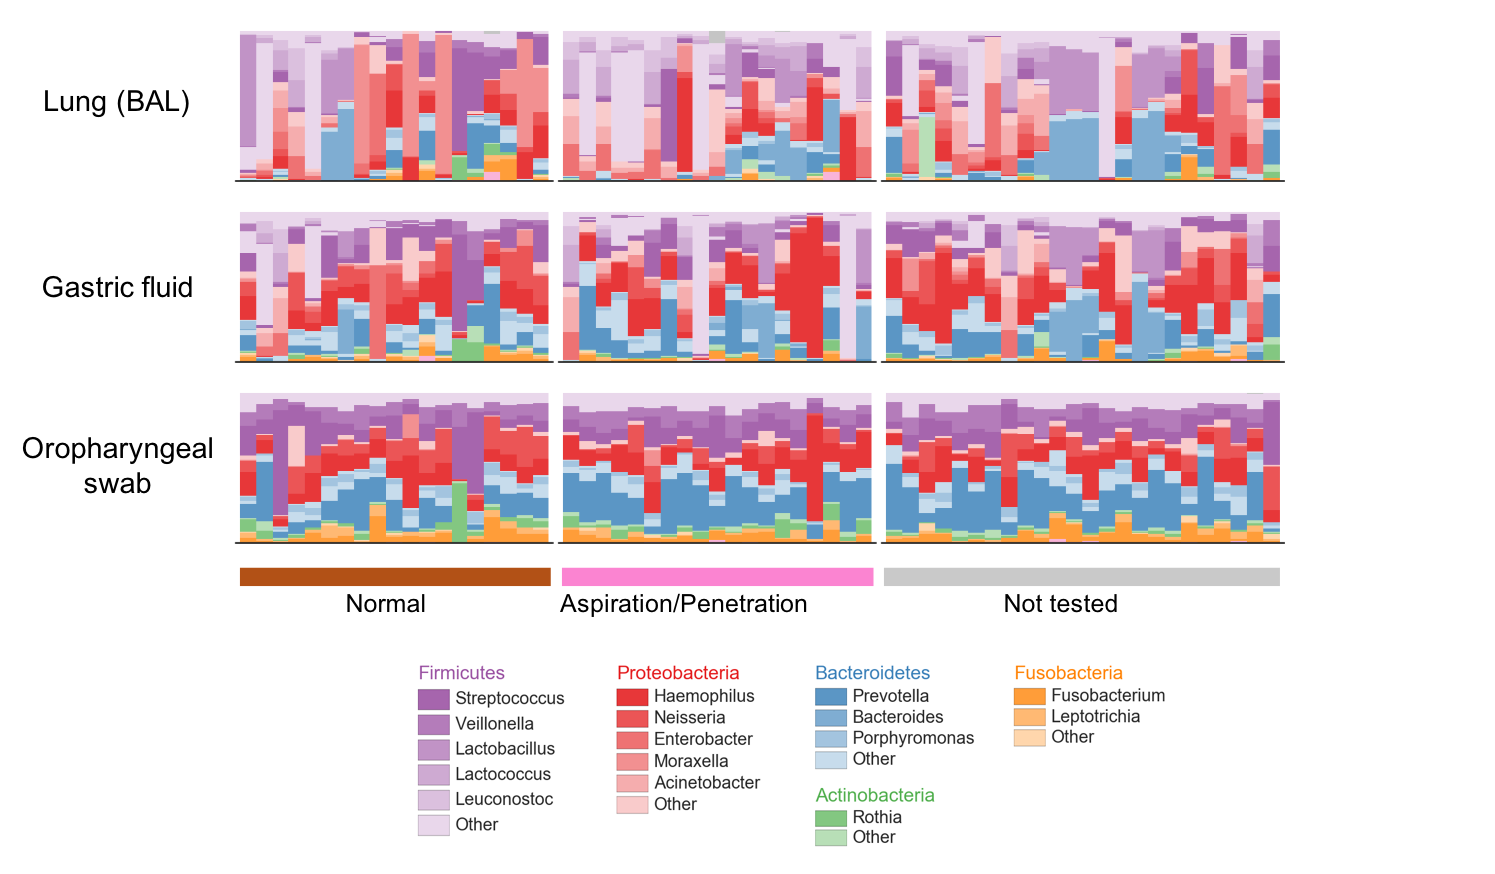
\includegraphics[width=1.2\textwidth]{community_overview_whitebckg.png}
        \caption{\textbf{Aerodigestive communities have similar predominant genera.} Bar plots showing relative abundances of aerodigestive OTUs collapsed to the genus level. Each column corresponds to one patient who had all three aerodigestive sites sequenced (N $=$ 19 non-aspirators, 23 aspirators, 24 untested). Phyla in legend are those with mean abundance $>$ 0.01 across all patients. Any other phyla are colored gray.}
        \label{fig1}
        \end{center}
\end{figure}

\begin{figure}[h]
        \begin{center}
        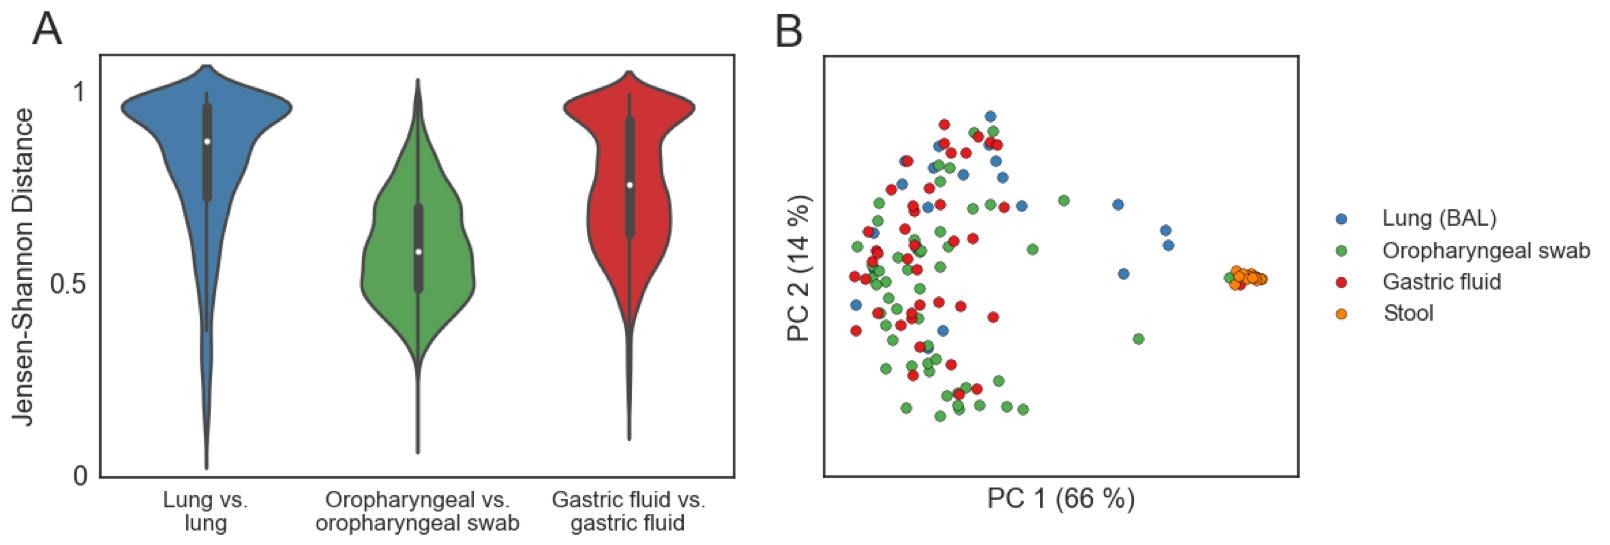
\includegraphics[width=\textwidth]{baseline_aerodigestive_across_patients_whitebckg.png}
        \caption{\textbf{Lung and gastric communities are more variable across people than oropharyngeal communities.} (A) Violin plot of the Jensen-Shannon distance (JSD) between samples from the same site across different patients. A JSD close to 1 indicates that communities are very different (less similar). (B) PCoA plots of aerodigestive and stool microbial communities for all patients in the 2016 sequencing batch (N $=$ 21 BAL, 52 oropharyngeal swab, 43 gastric fluid, and 14 stool samples).}
        \label{fig2}
        \end{center}
\end{figure}

\begin{figure}[h]
        \begin{center}
        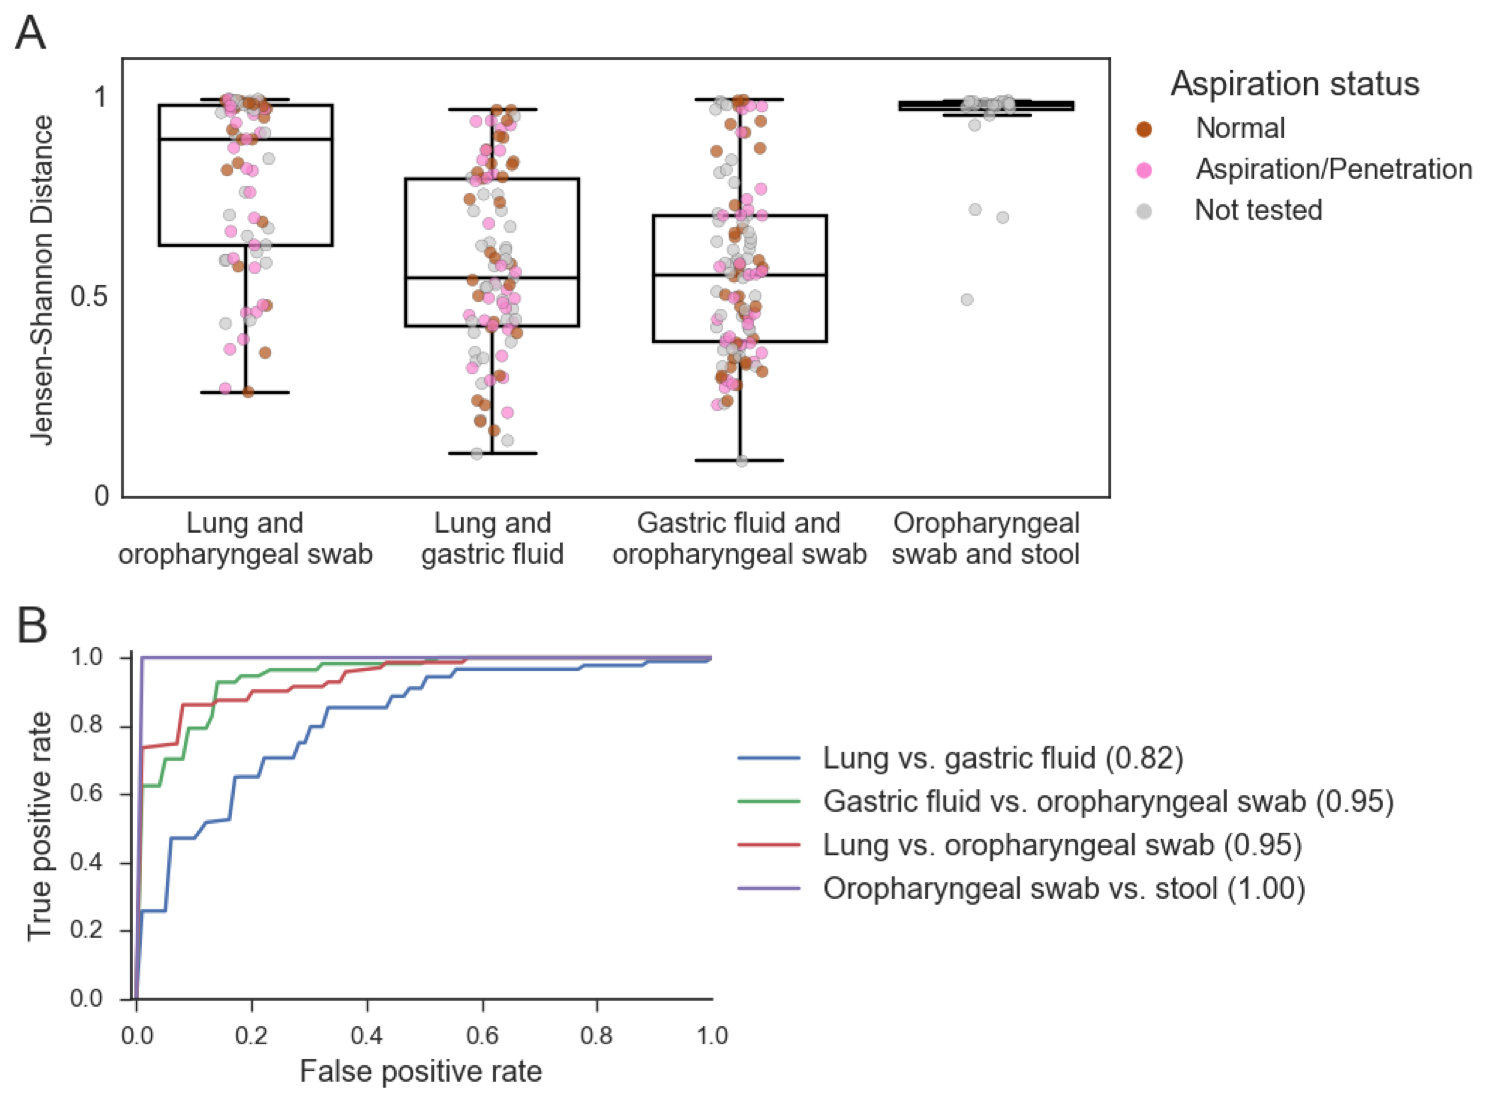
\includegraphics[width=\textwidth]{baseline_aerodigestive_within_patients_whitebckg.png}
        \caption{\textbf{Within patients, aerodigestive communities are similar but lung and oropharynx remain most distinct.} (A) Jensen-Shannon distances between samples from different sites from the same patient. Comparisons between stool and oropharynx are included to contextualize these results, as these are expected to be very different. All comparisons are significant (Wilcoxon rank sums test calculated with Python's \texttt{scipy.stats.ranksums} function) except the lung and gastric fluid vs. gastric fluid and oropharyngeal swab beta diversities (p $=$ 0.6). Lung and oropharyngeal vs. oropharyngeal and stool, p $=$ 0.005. All other comparisons:  $p < 1 \times 10^{-8}$. (B) ROC curve of classifiers distinguishing different aerodigestive sites. Mean areas under the ROC curve (AUCs) are reported in parentheses in the legend.}
        \label{fig3}
        \end{center}
\end{figure}

\begin{figure}[h]
        \begin{center}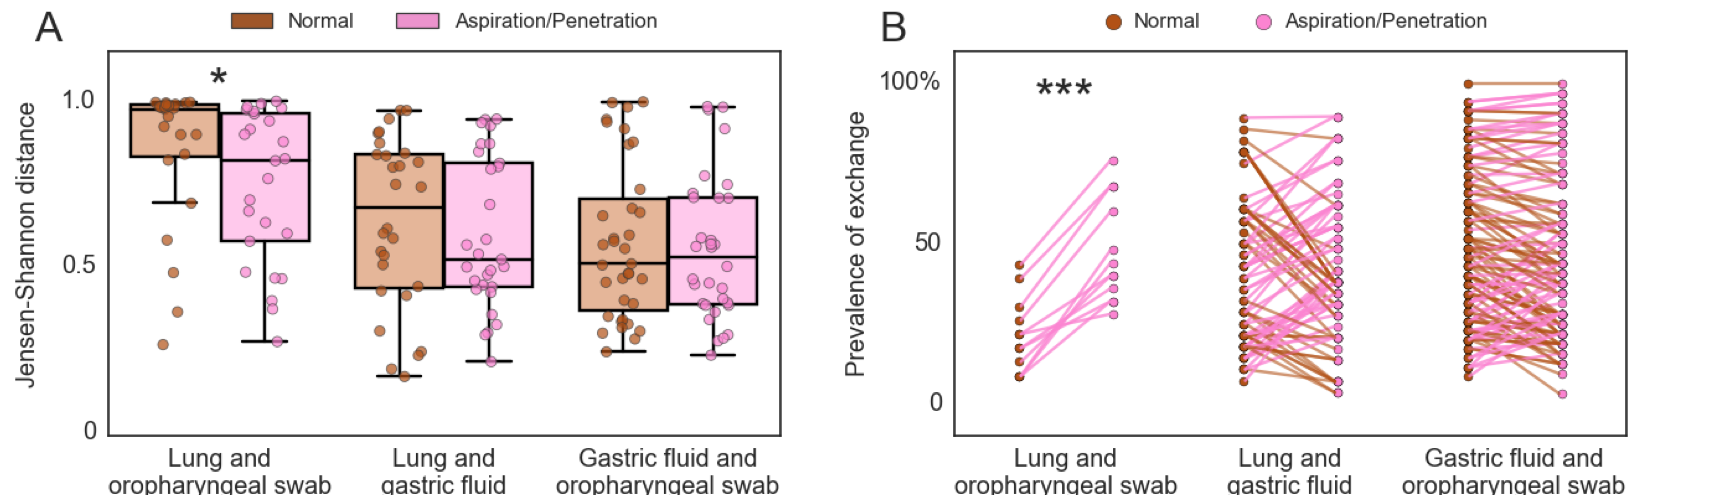
\includegraphics[width=\textwidth]{aspiration_jsd_exchange_whitebckg.png}
        \caption{\textbf{Dysphagia increases aspiration of microbes from the oropharynx but not the stomach} (A) Intra-patient Jensen Shannon distance for different aerodigestive site comparisons in non-aspirators (brown) and aspirators (pink). Each point represents one patient. P-values (Wilcoxon rank sums test, calculated with Python's \texttt{scipy.stats.ranksums} function): lung and oropharyngeal swab $p = 0.04$, lung and gastric fluid $p = 0.5$, gastric fluid and oropharyngeal swab $p = 0.8$. (B) Percentage of patients with the previously defined exchanged microbes present in both of the respective sites (x-axis) in non-aspirators (brown) and aspirators (pink). Each pair of points represents one exchanged OTU. P-values (paired t-test on $log_{10}$ prevalence values, calculated with Python's \texttt{scipy.stats.ttest\_rel} function: lung and oropharyngeal swab $p = 3 \times 10^{-5}$, lung and gastric fluid $p = 0.8$, gastric fluid and oropharyngeal swab $p = 0.09$.}
        \label{fig4}
        \end{center}
\end{figure}

\begin{figure}[h]
        \begin{center}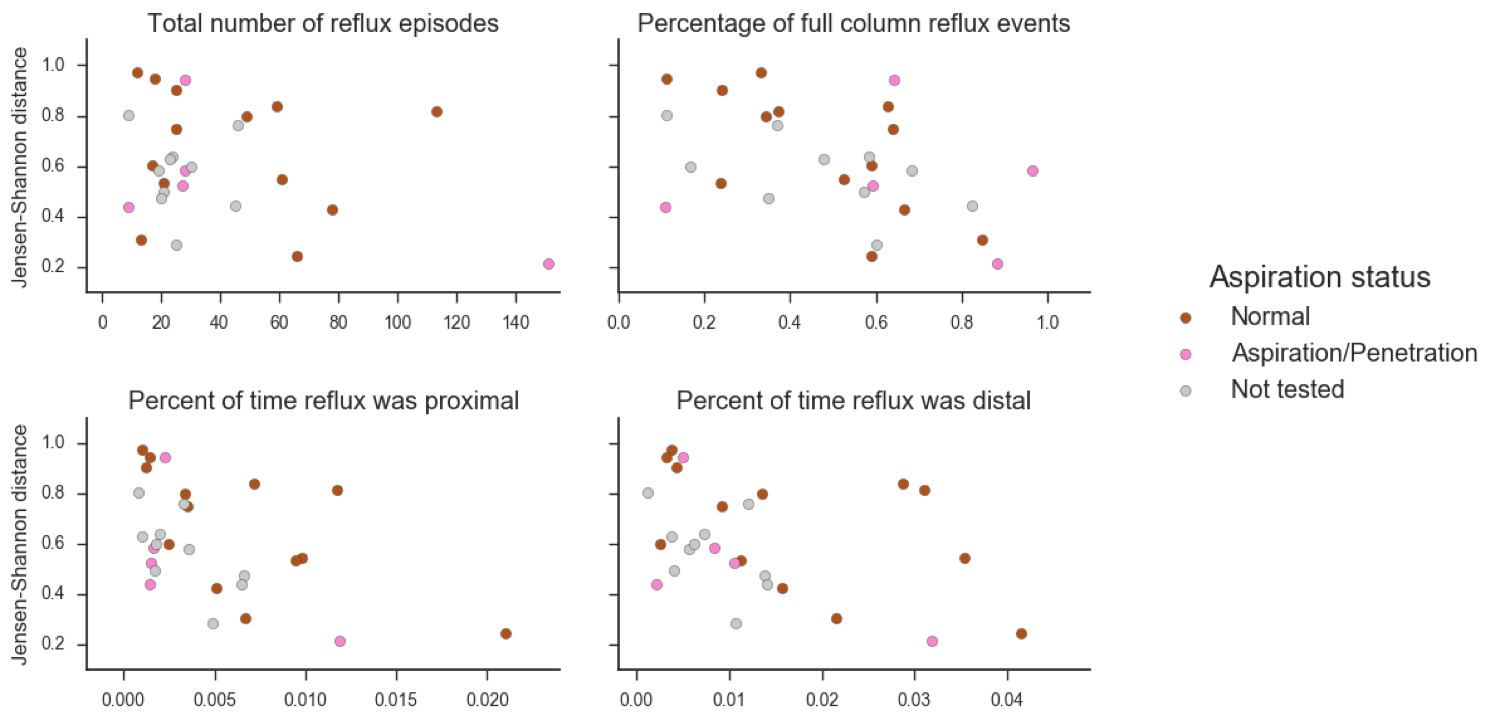
\includegraphics[width=\textwidth]{reflux_correlation_with_bal_gastric.png}
        \caption{\textbf{Reflux severity may correlate with the similarity between lung and gastric communities.} Each plot shows the correlation between different reflux measures and the within-patient Jensen-Shannon distance between BAL and gastric fluid samples. Points are colored according to aspiration status. All reflux measures include both acid- and non-acid reflux. Spearman correlation and p-values: total number of reflux episodes $\rho_s = -0.14, p = 0.5$, percentage of full column reflux events $\rho_s = -0.41, p = 0.03$, percent of time reflux was proximal $\rho_s = -0.47, p = 0.01$, percent of time reflux was distal $\rho_s = -0.43, p = 0.02$.}
        \label{fig5}
        \end{center}
\end{figure}

\FloatBarrier
\newpage

\bibliographystyle{unsrtnat}
\bibliography{aspiration/aspiration_refs.bib}

%\end{document}


%% This is an example first chapter.  You should put chapter/appendix that you
%% write into a separate file, and add a line \include{yourfilename} to
%% main.tex, where `yourfilename.tex' is the name of the chapter/appendix file.
%% You can process specific files by typing their names in at the
%% \files=
%% prompt when you run the file main.tex through LaTeX.

\graphicspath{{meta-analysis/figures/}}

\chapter{Meta-analysis of gut microbiome studies identifies disease-specific and shared responses}

Claire Duvallet, Sean M Gibbons, Thomas Gurry, Rafael A Irizarry, and Eric J Alm.

\bigskip
\bigskip
\noindent
The contents of this chapter were published as: ``Meta-analysis of gut microbiome studies identifies disease-specific and shared responses'' in \textit{Nature Communications} (2017) volume 8, article number 1784.

\bigskip
\bigskip
\noindent
The figures are at the end of the chapter. The Supplementary Information is in Appendix B.

\clearpage

%\usepackage[colorlinks=true]{hyperref} % for links and urls
%\usepackage{amsmath,amssymb} % for math
%\usepackage{color,soul} % for highlighting
%\usepackage{booktabs,rotating,multirow} % for nice tables
%\usepackage{authblk} % for author affiliations
%\usepackage{graphicx} % for figures
%\usepackage[numbers]{natbib}
%\usepackage[superscript,biblabel]{cite} % for superscript citations
%\usepackage[above]{placeins} % for FloatBarrier
%\usepackage{amsmath} % for pretty fraction text (heatmap caption)
%\usepackage{lineno} % for line numbers
%\usepackage{geometry} % for supp fig large pages

%% Smaller captions
%\usepackage[font=footnotesize]{caption}

\section*{Abstract}
Hundreds of clinical studies have demonstrated associations between the human microbiome and disease, yet fundamental questions remain on how we can generalize this knowledge.
Results from individual studies can be inconsistent and comparing published data is further complicated by a lack of standard processing and analysis methods.
Here, we introduce the MicrobiomeHD database, which includes 28 published case-control gut microbiome studies spanning ten diseases.
We perform a cross-disease meta-analysis of these studies using standardized methods.
We find consistent patterns characterizing disease-associated microbiome changes.
Some diseases are associated with over 50 genera, while most show only 10 to 15 genus-level changes.
Some diseases are marked by the presence of potentially pathogenic microbes whereas others are characterized by a depletion of health-associated bacteria.
Furthermore, we show that about half of genera associated with individual studies are bacteria which respond to more than one disease.
Thus, many associations found in case-control studies are likely not disease-specific but rather part of a non-specific, shared response to health and disease.

\newpage

\section{Introduction}

The human gastrointestinal tract digests food, absorbs nutrients, and plays important roles in maintaining metabolic homeostasis.
The microbes residing in our gut harvest energy from the food we eat, train our immune system, break down xenobiotics and other foreign products, and release metabolites and hormones important for regulating our physiology \cite{nash-baker, asd-kb, turnbaugh2006obesity}.
Chemical signals from our microbiota can act locally within the gut, and can also have larger systemic effects (e.g. the `gut-brain axis') \cite{Hsiao2013gutbrain,Cryan2012gutbrain,Poutahidis2013gutbrain}.

Due to the physiological interplay between humans and our microbial communities, many diseases are hypothesized to be associated with shifts away from a ``healthy'' gut microbiome.
These include metabolic disorders, inflammatory and auto-immune diseases, neurological conditions, and cancer, among others \cite{nash-baker, turnbaugh2006obesity, asd-son, crc-zhao, par-schep}.
Certain gut-related conditions (e.g. obesity and inflammatory bowel disease) have been extensively studied in human cohorts and in animal experiments, where significant and sometimes causal microbial associations have been shown.
These studies have spurred research into a number of complex diseases with unclear etiologies where a connection to the microbiome is suspected.

Overall, our current understanding of the precise relationships between the human gut microbiome and disease remains limited.
Existing case-control studies often report finding disease-associated microbial ``dysbiosis''.
However, the term ``dysbiosis'' is inconsistently and often vaguely defined, and can have a wide range of interpretations \cite{olesen2016dysbiosis,zaneveld2017karenina}.
Thus, we lack a comprehensive understanding of precisely how microbial communities and specific microbes within those communities cause, respond to, or contribute to disease.
Are different diseases characterized by distinct shifts in the gut microbiome?
Are some diseases marked by an invasion of pathogens whereas others show a depletion of beneficial bacteria?
Can we identify microbial biomarkers for certain conditions, which are consistently enriched or depleted in a disease across many patient cohorts?
Finally, are some bacteria part of a non-specific ``healthy'' or ``diseased'' microbiome and consistently associated with health or disease in general?

One approach to synthesize existing knowledge is to identify consistencies across studies through a meta-analysis, which allows researchers to find and remove false positives and negatives that may obscure underlying biological patterns.
However, prior meta-analyses of case-control gut microbiome studies have yielded mixed results and did not contextualize their findings across multiple diseases \cite{walters2014meta, Sze07092016,finucane2014obesity}.
For some conditions like inflammatory bowel disease (IBD), an overall difference in the gut microbiota was found within several studies, but no individual microbes were consistently associated with IBD across studies \cite{walters2014meta}.
For other conditions like obesity, multiple meta-analyses have found little to no difference in the gut microbiomes of obese and lean patients \cite{walters2014meta,Sze07092016,finucane2014obesity}, even though the microbiome has been causally linked to obesity in mouse models \cite{turnbaugh2006obesity, ridaura2013gut}.
These meta-analyses have been limited by focusing on only one or two diseases, and thus do not extend their findings across a broader landscape of human disease to answer more general questions about overall patterns of disease-associated microbiome shifts.

In this paper, we collected 28 published case-control 16S amplicon sequencing gut microbiome datasets spanning ten different disease states.
We acquired raw data and disease metadata for each study and systematically re-processed and re-analyzed the data.
We investigated whether consistent and specific disease-associated changes in gut microbial communities could be identified across multiple studies of the same disease.
Certain diseases (e.g. colorectal cancer (CRC)) are marked by an enrichment of disease-associated bacteria, while others (e.g. IBD) are characterized by a depletion of health-associated bacteria.
Some conditions (e.g. diarrhea) exhibit large-scale community shifts with many associated microbes, while most show only a handful of associations.
However, many associations are not specific to individual diseases but rather respond to multiple disease states.
In most studies, the majority of the individual disease-associated microbes were part of this set of bacteria that respond non-specifically to healthy and diseased states.
Thus, associations from individual case-control studies should be interpreted with caution, as these microbes may be indicative of a shared response to disease rather than part of disease-specific differences.
Together, these findings reveal distinct categories of dysbioses which can inform the development of microbiome-based diagnostics and therapeutics.

\section{Results}

\subsection{Most disease states show altered microbiomes}

To answer questions about the reproducibility and generalizability of reported associations between the human microbiome and disease, we collected, re-processed, and re-analyzed raw data from a collection of microbiome datasets.
We included studies with publicly available 16S amplicon sequencing data (i.e. FASTQ or FASTA) for stool samples from at least 15 case patients which also had associated disease metadata (i.e. case or control disease labels).
Studies which exclusively focused on children under 5 years old were excluded from our analyses.
We identified over 50 suitable case-control 16S datasets, of which 28 were successfully downloaded, processed, and included in a publicly available database which we called MicrobiomeHD \cite{microbiomehd}.
Characteristics of these datasets, including sample sizes, diseases and conditions, and references, are shown in Table \ref{tab:datasets} and Supplementary Table \ref{tab:datasets_full_info}.
For each downloaded study, we processed the raw sequencing data through our 16S processing pipeline (\url{https://github.com/thomasgurry/amplicon_sequencing_pipeline}) (see Supplementary Tables \ref{tab:processing} and \ref{tab:data} for detailed data sources and processing methods).
100\% denovo OTUs were assigned taxonomy with the RDP classifier \cite{wang2007naive} (c $=$ 0.5), converted to relative abundances by dividing by total sample reads, and collapsed to the genus level. OTUs which were not assigned at the genus level were discarded.
By collapsing data to the genus level, we lost the sensitivity to detect fine-scale differences in species or strain abundances across case and control groups, but we minimized certain batch effects that plague comparisons across studies.
Thus, we took a course-grained approach to optimize our ability to compare data across studies at the expense of phylogenetic resolution.

We first asked whether reported associations between the gut microbiome and disease would be recapitulated once we controlled for processing and analysis approaches.
To test whether the gut microbiome is altered in a variety of disease states, we built genus-level random forest classifiers to classify cases from controls within each study.
We compared the resulting area under the Receiver Operating Characteristic (ROC) curves (AUC) across studies (Figure \ref{fig:fig1}A, Supplementary Figure \ref{fig:roc_curves}).
We could classify cases from controls (AUC $>$ 0.7) for at least one dataset for all diseases except arthritis and Parkinson's disease, which each only had one study.
Notably, all diarrhea datasets (except Youngster et al. (2014) \cite{cdi-youngster}, which had only 4 distinct control patients and thus was not included in this analysis) had very high classifiability (AUC $>$ 0.9).
We successfully classified patients from controls (AUC $>$ 0.7) in three out of four IBD studies and all four CRC studies, which is consistent with previous work showing that these patients can be readily distinguished from controls using supervised classification methods \cite{walters2014meta,ibd-papa,crc-baxter,crc-zeller}.
Thus, the microbiome is indeed altered in many different diseases.

\subsection{Loss of beneficial microbes or enrichment of pathogens}

We next wondered whether the specific type of alteration was consistent across independent cohorts of patients with the same disease.
We performed univariate tests on genus-level relative abundances for each dataset independently and compared results across studies (Kruskal-Wallis (KW) test with the Benjamini-Hochberg false discovery rate (FDR) correction \cite{benjamini-hochberg}).
Our re-analyses of the studies were largely consistent with the originally reported results.
The same taxonomic groups showed similar trends as in the original publications, despite differences in data-processing methodologies (see Supplementary Note \ref{sec:lit_comp} for a full comparison of our re-analysis with previously published results).
Furthermore, we found that the disease-associated changes in the microbiome could be categorized into meaningful groups which provide insight into possible etiologies or therapeutic strategies for different types of disease.

In some diseases, microbiome shifts are dominated by an enrichment of a small number of ``pathogenic'' bacteria.
In these cases, it is possible that the microbes play a causal role and that they could be targeted with narrow-spectrum antimicrobials.
Colorectal cancer is characterized by such a shift, and we found significant agreement across three of the four CRC studies \cite{crc-zhao,crc-baxter,crc-zeller,crc-xiang} (Figures \ref{fig:fig1}B and \ref{fig:fig2}, genus labels in Supplementary Figure \ref{fig:supp_dis_specific}).
Dysbiosis associated with CRC is generally characterized by increased prevalence of the known pathogenic or pathogen-associated \textit{Fusobacterium}, \textit{Porphyromonas}, \textit{Peptostreptococcus}, \textit{Parvimonas}, and \textit{Enterobacter} genera (i.e. these genera were higher in CRC patients in 2 or more studies, Figures \ref{fig:fig2} and \ref{fig:fig3}A, genus labels in Supplementary Figures \ref{fig:supp_dis_specific} and \ref{fig:supp_meta_heatmap}).
\textit{Fusobacterium} is associated with a broad spectrum of human diseases and \textit{Porphyromonas} is a known oral pathogen \cite{Han2015fusopatho, Flynn2016oral}.

By contrast, other disease-associated microbiome shifts are characterized by a depletion of health-associated bacteria in patients relative to controls.
In these cases, probiotics that replace missing taxa may be a better treatment strategy than anti-microbials.
Across our four IBD studies, patient microbiomes were dominated by a depletion of genera in patients relative to controls, especially butyrate-producing \textit{Clostridiales} \cite{ibd-papa,ibd-gevers,ibd-hut,ibd-engstrand} (Figures \ref{fig:fig1}B and \ref{fig:fig2}, genus labels in Supplementary Figure \ref{fig:supp_dis_specific}).
In particular, five genera from the \textit{Ruminococcacaea} and \textit{Lachnospiracaea} families were consistently depleted in IBD patients relative to controls in at least two studies (Figure \ref{fig:fig3}A, genus labels in Supplementary Figure \ref{fig:supp_meta_heatmap}).
While not all genera within \textit{Ruminococcacaea} and \textit{Lachnospiracaea} are verified short-chain fatty acid (SCFA) producers, the dominant genera within these families are known to harbor genes for short chain fatty acid production \cite{louis2010diversity} and are often associated with colonic health \cite{flint2012role,miquel2013faecalibacterium,reeves2012suppression}.
We found similar results when comparing Crohn's disease and ulcerative colitis patients to controls separately, without any consistent patterns across datasets that distinguished either IBD sub-type (Supplementary Note \ref{sec:split_cases}; Supplementary Figures \ref{fig:split_cases_fig1} and \ref{fig:split_cases_heatmaps}).

Some conditions are characterized by a broad restructuring of gut microbial communities.
In these cases, full community restoration strategies like fecal microbiota transplants may be more appropriate.
For example, diarrhea consistently results in large-scale rearrangements in the composition of the gut microbiome, which is likely reflective of reduced stool transit time (Figures \ref{fig:fig1} and \ref{fig:fig2}).
We saw many microbes consistently associated with both \textit{Clostridium difficile} infection (CDI) and non-CDI diarrhea (Figures \ref{fig:fig2} and \ref{fig:fig3}A) \cite{cdi-youngster,cdi-schubert,cdi-vincent,edd-singh}.
In general, Proteobacteria increase in prevalence in patients with diarrhea, with a concomitant decrease in the relative abundances of Bacteroidetes and some Firmicutes.
In particular, we see a reduction in butyrate-producing Clostridia, including genera within \textit{Ruminococcaceae} and \textit{Lachnospiraceae} families, which have been associated with a healthy gut \cite{wong2006colonic}.
We also see an increase in prevalence of genera that contain organisms often associated with lower pH and higher oxygen levels of the upper-gut, like \textit{Lactobacillaceae} and \textit{Enterobacteriaceae}, in patients with diarrhea (Figure \ref{fig:fig3}A) \cite{donaldson2016gut}.
Additionally, both CDI and non-CDI diarrhea patients had lower alpha diversity, a measure of overall community structure, than healthy controls in all studies (Supplementary Figures \ref{fig:fig_alpha}-\ref{fig:fig_alpha_simpson}).
Consistent with the CDI and non-CDI diarrheal studies, we also found that organisms associated with the upper gut, like \textit{Lactobacillus} and \textit{Enterobacteriaceae}, appear to be enriched in IBD patients, who can present with diarrheal symptoms (Supplementary Figure \ref{fig:supp_dis_specific}) \cite{donaldson2016gut,Kirsner1982ibd}.
IBD patients also tended to have lower alpha diversities than controls (Crohn's disease vs. controls in three studies, ulcerative colitis vs. controls in two studies; Supplementary Figures \ref{fig:fig_alpha}--\ref{fig:fig_alpha_simpson}), though this difference was less drastic than in the diarrheal studies where all patients had active diarrhea.

In some studies, confounding variables may drive associations.
For example, there were no consistent differences between cases and controls across HIV studies because of demonstrated confounders \cite{noguera2016gut,lozupone2013alterations,hiv-dinh} (Figure \ref{fig:fig2}, \ref{fig:fig3}A).
As in the original Lozupone et al. (2013) \cite{lozupone2013alterations} study, we found enrichment in \textit{Prevotella}, \textit{Catenibacterium}, \textit{Dialister}, and \textit{Desulfovibrio} in HIV-positive patients, in addition to 8 other genera (Figure \ref{fig:fig2} and Supplementary Figure \ref{fig:supp_dis_specific}).
We also found depletion of \textit{Bacteroides}, \textit{Odoribacter}, \textit{Anaerostipes}, \textit{Parasutterella}, and \textit{Alistipes} in HIV-positive patients relative to controls.
However, the Noguera-Julian et al. (2016) study showed that the genera that were significantly associated with HIV in the Lozupone paper were strongly associated with sexual behavior (e.g. men who have sex with men were associated with much higher \textit{Prevotella} levels), and our re-analysis also found conflicting results between these two studies (Figure \ref{fig:fig2}).
Thus, there is no consensus on what genera are associated with HIV.
Obesity is another example where confounding variables may drive microbiome alterations.
Three recent meta-analyses found no reproducible obesity-associated microbiome shifts \cite{walters2014meta,Sze07092016,finucane2014obesity}, which is consistent with our classification results where we were only able to accurately classify obese and control patients in two out of five studies (Zhu et al. (2013) \cite{nash-baker}, Turnbaugh et al. (2009) \cite{ob-gordon}; Figure \ref{fig:fig1}A).
Our genus-level re-analysis did find a few consistent genus-level associations between lean and obese patients \cite{nash-baker,ob-gordon,ob-goodrich,ob-zupancic,ob-ross}.
Two genera, \textit{Roseburia} and \textit{Mogibacterium}, were significantly enriched in obese individuals across two of the obesity studies (Figure \ref{fig:fig3}A).
Furthermore, \textit{Anaerovorax}, \textit{Oscillibacter}, \textit{Pseudoflavonifractor}, and \textit{Clostridium IV}  were depleted in obese patients relative to controls in two of the studies.
However, two of the five studies had no significant genus-level associations (q $<$ 0.05), despite one having a large sample size (Zupancic et al. (2012) \cite{ob-zupancic}).
This suggests that confounding factors like diet may have given rise to certain associations found in our re-analysis and previously reported in the literature \cite{finucane2014obesity}.
More studies that control for potential confounders, like host behavior and diet, will be required for diseases like obesity and HIV, where associations with the microbiome remain unclear.
Finally, patients in case-control cohorts are frequently on other medications such as antibiotics which may confound disease-associated microbiome shifts.
Six of our datasets included antibiotics metadata, and of these only one dataset (Schubert et al, 2014 \cite{cdi-schubert}) had more than 5 controls who were on antibiotics.
Thus, it is very likely that disease-associated genera in conditions which are often treated with antibiotics (e.g. diarrhea, IBD) are confounded with antibiotic usage.
Future case control studies should focus on better separating treatment and disease variables by collecting detailed metadata on antibiotic and other medication usage, and perhaps also by recruiting controls undergoing a variety of treatments.

\subsection{Shared vs. disease-specific microbial responses}

Finally, we sought to determine whether a unified microbiome response to general health and disease could be identified.
Previous studies have proposed that reduced alpha diversity is a reliable indicator of disease-associated dysbiosis \cite{cdi-vincent,ob-gordon,mosca2016gut}.
In our re-analysis, we found no consistent reduction of alpha diversity in case patients, with the exception of diarrhea and perhaps IBD (Supplementary Figures \ref{fig:fig_alpha}--\ref{fig:fig_alpha_simpson}).
These results are consistent with previous meta-analyses, which found inconsistent relationships between alpha diversity and disease and very small effect sizes in non-diarrheal diseases \cite{walters2014meta, Sze07092016}.
To further address the question of whether we could find a robust, generalized signal for diseased microbiomes regardless of the disease type, we built random forest classifiers to distinguish healthy patients from any type of case patient.
The AUCs from these general healthy vs. disease classifiers correlated strongly with the original single-dataset classification results, indicating that there is indeed a general microbiome signal that can be identified even across different diseases (see Supplementary Note \ref{sec:overall_classifier} and Supplementary Figure \ref{fig:overall_classifier}).

Having putatively shown the presence of a generalized microbial response to disease, we next sought to identify individual genera which respond non-specifically to health and disease.
We considered a genus to be part of the non-specific, shared microbial response if it was significantly enriched or depleted (q $<=$ 0.05) in at least one dataset from at least two different diseases (see Supplementary Note \ref{sec:core_defns} and Supplementary Figures \ref{fig:core_defns} and \ref{fig:core_sig} for further discussion on alternative definitions and statistical significance of shared response).
We identified 24 health-associated genera and 20 disease-associated genera out of the 152 genera that were significant in at least one dataset (Figure \ref{fig:fig3}A, genus labels in Supplementary Figure \ref{fig:supp_meta_heatmap}).
We also found 7 genera that were both health- and disease-associated (i.e. they were enriched in controls across at least two diseases, but were also depleted in controls in different comparisons across at least two diseases) (Figure \ref{fig:fig3}A, black).
Perhaps these genera represent bacteria disproportionately affected by confounders or technical artifacts.
Alternatively, different species or strains within these genera may play alternate roles across diseases or community contexts, giving rise to variable responses at the genus level.

We identified distinct sub-groups of microbes within the \textit{Bacteroidetes} and \textit{Firmicutes} phyla which respond non-specifically to health and disease (Figure \ref{fig:fig3}A).
The order \textit{Clostridiales} (specifically the \textit{Lachnospiraceae} and \textit{Ruminococcacaea} families) is associated with health across multiple diseases while the order \textit{Lactobacillales} and family \textit{Clostridiales Incertae Sedis XI} are associated with disease.
The majority of the the non-specific responders in the order \textit{Clostridiales} were associated with health, comprising the majority of all of the microbes which were non-specifically associated with healthy patients (17 genera out of 24 total health-associated genera).
All of five of the non-specific responders in the order \textit{Lactobacillales} were enriched in case patients across multiple diseases.
\textit{Lactobacillales} genera are adapted to the lower pH of the upper gastrointestinal tract \cite{donaldson2016gut}.
Perhaps the shared disease-associated taxa are indicators of shorter stool transit times and disruptions in the redox state and/or pH of the lower intestine, rather than specific pathogens.
These non-specific responders are consistent with the results from a recent meta-analysis of six metagenomics datasets, which also found \textit{Lactobacillales} and \textit{Clostridiales} microbes among the most discriminative classification features across multiple studies \cite{pasolli2016machine}.
Finally, we found that the order \textit{Bacteroidales} is more mixed: two \textit{Bacteroidales} genera were non-specifically associated with health, one with disease, and two with both health and disease.

A majority of bacterial associations within individual studies overlap with the shared response.
For each dataset that had at least one significant (q $<$ 0.05) association, we calculated the percent of associated genera which were also part of the non-specific response in the same direction (Figure \ref{fig:fig3}B).
Strikingly, the majority of microbial responses were not specific to individual diseases; on average, 51\% of a dataset's genus-level associations were genera which were associated with more than one disease.
In light of this finding, it is important that researchers performing future case-control studies consider whether an identified microbial association is truly specific to their disease of interest or is instead responding to a common symptom (e.g. diarrhea) or perhaps generally associated with health or sickness.
Additionally, they can use the knowledge that many microbes respond non-specifically to disease to narrow lists of putative causal or diagnostic biomarkers to microbes which fall outside of the shared response and are thus more likely to be specific to the disease being studied.
Researchers can access an updated list of shared microbial responders from this analysis at the MicrobiomeHD database \cite{microbiomehd}, or they can curate their own lists by performing similar cross-disease meta-analyses.

Bacteria which are non-specifically associated with health are both ubiquitous and abundant across people, whereas bacteria which are non-specifically associated with disease are abundant when present but are not ubiquitous.
We calculated the average relative abundance (i.e. the total relative abundance across all patients divided by the number of patients with non-zero abundance) and ubiquity (i.e. the number of patients with non-zero abundance divided by the total number of patients) for each genus in the shared response.
We found that health-associated genera were more ubiquitous than disease-associated ones, but not necessarily more abundant (Figure \ref{fig:fig3}C).
Thus, presence/absence of the non-specifically disease-associated genera appears to be a better indicator of disease-associated microbial shifts than changes in their relative abundances.
However, a small subset of the non-specifically disease-associated genera were relatively ubiquitous across patients.
Among the most ubiquitous were \textit{Escherichia/Shigella} and \textit{Streptococcus}.
\textit{Escherichia} includes common commensal strains, as well as pathogenic strains \cite{rasko2008pangenome}, and is frequently present in healthy people's guts as well as over-represented in sick patients. Genera within \textit{Enterobacteriaceae}, \textit{Lactobacillaceae}, and \textit{Streptococcaceae} families are dominant in the upper gastrointestinal tract \cite{donaldson2016gut,wang2013upper} and are present in many people's stool at low frequency. These taxa likely become enriched with faster stool transit time (i.e. signatures of diarrhea) \cite{donaldson2016gut,savage1977microbial}.


\subsection{Within and cross-disease meta-analysis improves interpretability}

Identifying disease-specific and non-specific microbial responses required comparing studies both within and across multiple diseases.
Multiple studies of the same disease were necessary to identify shifts consistently associated with individual diseases.
We did not find consistent bacterial associations for conditions with fewer than four datasets (Figure \ref{fig:fig1}, \ref{fig:fig3}A).
Within-disease meta-analysis also increased our ability to interpret the results from any one dataset.
Despite few significant differences, some of these studies (e.g. Zhang et al. (2013) \cite{mhe-zhang}, Zhu et al. (2013) \cite{nash-baker}) had high classifiability of patients vs. controls (AUC $>$ 0.7, Figure \ref{fig:fig1}A), indicating that there may be a disease-associated shift that was not detected by univariate comparisons.
However, because few other studies of the same disease were available for comparison, we could not confidently interpret the classification results beyond the reported AUC.
For other studies with high AUCs but few univariate associations (e.g. Vincent et al. (2013) \cite{cdi-vincent}, Morgan et al. (2012) \cite{ibd-hut}, Chen et al. (2012) \cite{crc-xiang}), our confidence that the high AUCs reflect true disease-associated differences increased because the high AUCs were consistent with other classifiers from the same disease type.

Meta-analysis identified potential false positives and false negatives across studies and conditions.
For example, we found that reported associations between alpha diversity and disease within individual studies tended to lose significance when looking across studies, except in the case of diarrhea and perhaps IBD (Supplementary Figures \ref{fig:fig_alpha}--\ref{fig:fig_alpha_simpson}).
Another example of a potential false positive was the association between \textit{Prevotella} and disease.
Autism \cite{asd-kb}, rheumatoid arthritis \cite{ra-littman}, and HIV \cite{lozupone2013alterations,hiv-dinh} have each been reported to be associated with \textit{Prevotella}. For each of these diseases, the associations with \textit{Prevotella} were weakly significant or complicated by confounding factors.
In our more statistically conservative re-analysis, we found no association between autism or arthritis and \textit{Prevotella}.
As mentioned previously, in the case of HIV, the association with \textit{Prevotella} was due to demographic factors unrelated to disease \cite{noguera2016gut}.
Regardless of whether shifts in \textit{Prevotella} are truly biologically related to each studied disease state, it is clear that such shifts are not specific to one particular condition and should not be reported as putative disease-specific biomarkers.
We also found that certain signals picked out by meta-analysis did not always hold within individual studies.
For example, studies with small sample sizes often had few or no significant associations (e.g. Vincent et al. (2014) \cite{cdi-vincent}, Chen et al. (2012) \cite{crc-xiang}, and Willing et al. (2009) \cite{ibd-engstrand}).
Here, the fact that other studies analyzing the same diseases consistently found associations strengthens the hypothesis that the lack of microbiome-associated signal in these studies was due to low power rather than a lack of true signal.
Because individual studies are plagued by low statistical power, confounding variables, and batch effects which can obscure biological signals, the identification of disease-specific and non-specific microbial associations will continue to improve as more datasets and diseases are included in future meta-analyses.


\section{Discussion}

Here, we report patterns of disease-associated shifts in the human gut microbiome which differ in their directionality (i.e. fraction of disease-enriched vs. disease-depleted genera) and extent (i.e. total number of genera that differ between cases and controls).
Some diseases are characterized by an invasion of pathogenic or disease-associated bacteria (e.g. CRC), while others largely show a depletion of health-associated microbes (e.g. IBD).
Diarrheal illnesses induce large-scale rearrangement of many members of the microbiota, whereas other conditions show fewer associations.
We also find a set of microbes which are non-specifically associated with multiple diseases and show that these microbes comprise many of the disease-associated genera within any given study.

The identification of a non-specific microbial response is an important concept that should be considered in future case-control microbiome studies.
It suggests that studies should be interpreted with extra caution, as many identified microbial associations may be indicative of a shared response to health or disease rather than a disease-specific biological difference.
Microbes that are non-specifically associated with multiple diseases would not be useful as disease-specific diagnostics or to address causality \cite{olesen2016dysbiosis}.
On the other hand, bacteria that are associated with healthy patients across multiple diseases could be developed into a general probiotic which may be suited for many different conditions.

Additionally, characterizing ``dysbioses'' by their directionality and extent is a useful framework to generate hypotheses for future research on complex, heterogenous diseases with links to the microbiome.
For example, the search for microbiome-based diagnostics may be more appropriate for diseases with consistently enriched disease-associated microbes, like CRC.
On the other hand, patients with diseases which are characterized by depletion of health-associated microbes, like IBD, may benefit from prebiotic or probiotic interventions designed to enrich for these taxa.
Furthermore, conditions which are characterized by large-scale shifts in community structure may be well-suited to treatment with fecal microbiota transplantation, as in CDI \cite{cdi-youngster}.
While many of these conditions are unlikely to be fully treated by antibiotics, probiotics, or fecal microbiota transplants, our proposed framework could guide the search for new therapies and etiologies by generating testable hypotheses with higher likelihoods of success \cite{olesen2016dysbiosis}.

This analysis is the first to compare microbiome studies across more than two different diseases and highlights the importance of making raw data and associated patient metadata publicly available to enable future, more comprehensive analyses.
This analysis does not include all possible studies, and certain important gastrointestinal diseases (e.g. irritable bowel syndrome) are missing, largely due to data and metadata availability.
Future studies should expand on this work by including more cohorts from the same diseases as well as more diseases.
To re-analyze these studies, we applied standard methods commonly used in the field and assumed that the original study designs and patient selection methods were adequate.
We were reassured to find that a straightforward and standardized approach was able to recover very similar results to those previously reported in the various papers.
Thus, we did not formally investigate heterogeneity between cohorts or technical inter-study batch effects.
However, it is clear from our genus-level results that there is significant variation even across studies of the same disease.
There are many possible reasons for this variation (experimental and sequencing artifacts, host-related covariates, stochastic disease-associated community changes etc. \cite{ zaneveld2017karenina,Falony2016variation, David2014lifestyle}), and future analyses should consider methods to correct for host confounders and technical batch effects.
Concerns about batch effects motivated us to analyze the data at the genus level, which necessarily limited our resolution and biological interpretations of identified associations (e.g. different species or strains within a genus may have different associations with disease, which would not be captured in this analysis).
Making raw data from case-control studies publicly available will also allow researchers to develop methods to correct for these batch effects, in addition to enabling more comprehensive future meta-analyses.

Despite the limitations of this study, our results provide more nuanced insight into dysbiosis, revealing distinct types of alterations that more precisely describe disease-associated microbiome shifts.
As the number of case-control cohorts increases, similar meta-analyses could be used to compare related diseases and identify microbiome alterations associated with general host physiological changes.
For example, there may be a group of microbes which respond to or cause systemic inflammation.
Could we identify these microbes by comparing multiple inflammatory or auto-immune diseases and study them to better understand the interactions between the microbiome and our immune system?
Furthermore, some microbes may be consistently associated with neurological conditions and could contribute to the gastrointestinal symptoms that accompany or precede neurological manifestations \cite{asd-kb,par-schep}.
Studying these microbes could help us understand the `gut-brain axis' by identifying common neuroactive molecules produced by these bacteria, which could also be used as targets for new treatments \cite{Hsiao2013gutbrain,Cryan2012gutbrain,Poutahidis2013gutbrain}.
Finally, meta-analysis could be used to identify subsets of patients who exhibit distinct microbiome shifts within heterogenous diseases like IBD or in conditions which exhibit stochastic microbial responses, allowing for further stratification of disease subtypes and microbiome disruptions \cite{zaneveld2017karenina,ibd-engstrand,Pascal2017crohns}.
This work demonstrates that employing standard methods to contextualize new results within the broader landscape of clinically relevant microbiome studies is feasible and adds value to individual analyses.
As excitement in this field grows, researchers should harness the increasing number of replicated case-control studies to swiftly and productively advance microbiome science from putative associations to transformative clinical impact.


\section{Methods}

\subsection{Dataset collection}

We identified case-control 16S studies from keyword searches in PubMed and by following references in meta-analyses and related case-control studies.
We included studies with publicly available raw 16S data (fastq or fasta) and metadata indicating case or control status for each sample.
Most data was downloaded from online repositories (e.g. SRA) or links provided in the original publications, but some were acquired after personal communication with the authors (Supplementary Table \ref{tab:data}).
We did not include any studies which required additional ethics committee approvals or authorizations for access (e.g. controlled dbGaP studies).
In studies where multiple body sites were sampled or where multiple samples were taken per patient, we also required the respective metadata to include those metadata.
We analyzed only stool 16S samples, and excluded studies with fewer than 15 case patients.
In CRC studies with multiple control groups (e.g. healthy and non-CRC adenoma), only the healthy patients were used as controls for all of our comparisons.
In studies with non-healthy controls (e.g. non-IBD patients), these patients were used as controls (as in the original papers).
In the Schubert et al. CDI study \cite{cdi-schubert}, which had both CDI and non-CDI diarrheal patients, each group was used as an independent case group compared with controls.
We also analyzed the NASH and obese patients from the Zhu et al. study \cite{nash-baker} as independent case groups.
When obesity studies reported body mass index instead of obesity status, we considered patients with BMI less than 25 as our control group and patients with BMI greater than 30 as the case group.

\subsection{16S processing}

Raw data were downloaded and processed through our in-house 16S processing pipeline ({\url{ https://github.com/thomasgurry/amplicon_sequencing_pipeline}).
Data and metadata were acquired as described in Supplementary Table \ref{tab:data}.
When needed, we de-multiplexed sequences by finding exact matches to the provided barcodes and trimmed primers with a maximum of 1 mismatch.
In general, sequences were quality filtered by truncating at the first base with Q $<$ 25.
However, some datasets did not pass this stringent quality threshold (i.e. the resulting OTU table was either missing many of the original samples, or the read depth was significantly lower than reported in the original paper).
For 454 data, we loosened the quality threshold to 20, whereas for paired-end Illumina data we removed reads with more than 2 expected errors.
If possible, all reads were trimmed to 200 bp.
In cases where this length trimming discarded a majority of sequences, we lowered our threshold to 150 or 101 bp.
The specific processing parameters we used for each dataset can be found in Supplementary Table \ref{tab:processing}.
To assign OTUs, we clustered OTUs at 100\% similarity using USEARCH \cite{edgar-usearch-2010} and assigned taxonomy to the resulting OTUs with the RDP classifier \cite{wang2007naive} and a confidence cutoff of 0.5.
For each dataset, we removed samples with fewer than 100 reads and OTUs with fewer than 10 reads, as well as OTUs which were present in fewer than 1\% of samples within a study.
We calculated the relative abundance of each OTU by dividing its value by the total reads per sample.
We then collapsed OTUs to genus level by summing their respective relative abundances, discarding any OTUs which were unannotated at the genus level.
All statistical analyses were performed on this genus-level relative abundance data.

\subsection{Statistical analyses}

To perform supervised classification of cases and controls within each dataset, we built Random Forest classifiers with 5-fold cross-validation.
To build our train and test sets, we used the python \texttt{scikit-learn} \texttt{StratifiedKFold} function with shuffling of the data \cite{scikit-learn}.
To build our classifiers, we used the \texttt{RandomForestClassifier} function with 1000 estimators and other default settings \cite{scikit-learn}.
We found no significant effect of various Random Forest parameters on the AUCs  (Supplementary Figures \ref{fig:rf_params_gini} and \ref{fig:rf_params_entropy}).
We calculated the interpolated area under the ROC curve (AUC) for each classifier based on the cross-validation testing results.
To account for spurious high classifiability due to class imbalances, we also calculated the Cohen's kappa score for each classifier using \texttt{sklearn.metrics.cohen\_kappa\_score} on the test set predictions (Supplementary Table \ref{tab:kappa}).
The kappa scores correlated well with the AUCs (Pearson $\rho$ $=$ 0.9), indicating that the majority of the classifiers performed well even when considering their underlying data distributions.
We excluded Youngster et al. (2014) \cite{cdi-youngster}, which had only 4 distinct control patients, from all classifier analyses.

We performed univariate analyses on the relative abundances of genera in cases and controls with a non-parametric Kruskal-Wallis test using the \\ \texttt{scipy.stats.mstats.kruskalwallis} function \cite{scipy}.
We corrected for multiple hypothesis testing in each dataset with the Benjamini-Hochberg false discovery rate \cite{benjamini-hochberg}.
We performed all analyses on genus-level relative abundances for each dataset individually, and then compared these results across all studies.

We considered a genus to be consistently associated with a disease (Figure \ref{fig:fig3}A, bottom) if it was significantly associated (q $<$ 0.05) with the disease in the same direction in at least two studies of that disease.
We considered a genus to be a non-specific microbial association (Figure \ref{fig:fig3}A, top) if it was significantly associated (q $<$ 0.05) in at least one dataset of at least two different diseases in the same direction.
When we defined these non-specific genera, we did not include datasets which used non-healthy controls (Papa et al. (2012) \cite{ibd-papa} and Gevers et al. (2014) \cite{ibd-gevers}) and the Lozupone et. al (2013) dataset \cite{lozupone2013alterations}, where the microbiome signal reflected behavior rather than disease state \cite{noguera2016gut}.

To build our generalized healthy vs. disease classifiers, we first concatenated metadata and genus-level abundance data for all datasets which had healthy controls (i.e. all datasets except Papa et al. (2012) \cite{ibd-papa} and Gevers et al. (2014) \cite{ibd-gevers}, which used non-IBD patients as controls, and CDI Youngster (2014), \cite{cdi-youngster}, which had only 4 distinct controls).
We performed leave-one-dataset-out and leave-one-disease-out cross validation and calculated an AUC for each of the testing results.

\subsection{Microbiome community analyses}

Alpha diversities were calculated based on the non-collapsed 100\% OTU-level relative abundances, and included un-annotated OTUs.
We calculated alpha diversity metrics with the \texttt{skbio.math.diversity.alpha.chao1}, \texttt{shannon}, and \texttt{simpson} implementations.

We calculated the average abundance and ubiquity (Figure \ref{fig:fig3}C) of each genus as the mean of its average values in each dataset across all patients.
To calculate the abundance of each genus, we first calculated each genus's mean abundance within each dataset.
We counted only patients with non-zero abundance of the genus in this calculation.
We then took the average of these mean abundances across all datatsets.
To calculate the ubiquity of each genus, we calculated the percent of patients with non-zero abundance of that genus in each dataset.
We then took the average of these ubiquities across all datasets.

\subsection{Code availability}

The code to reproduce all of the analyses in this paper is available at \url{https://github.com/cduvallet/microbiomeHD}.
We encourage researchers to incorporate their existing and future case-control studies into the MicrobiomeHD database by contacting us.

\subsection{Data availability}

Raw sequencing data for each study can be accessed as described in Supplementary Table \ref{tab:data}.
The raw processed OTU tables can be accessed at the MicrobiomeHD database, available at \url{https://doi.org/10.5281/zenodo.840333} \cite{microbiomehd}.

Supplementary files, including the q-values for all genus-level comparisons in every dataset, disease-associated genera for the diseases with more than three datasets, and a list of non-specific genera are also available at \url{https://github.com/cduvallet/microbiomeHD}.
All other relevant data supporting the findings of the study are available in this article and its Supplementary Information files, or from the corresponding author upon request.

\section{Acknowledgements}

We thank the authors who made their data publicly available as well as those who provided data after personal communication.
The Center for Microbiome Informatics and Therapeutics supported the computational resources for this project, and C.D. acknowledges support by the Department of Defense through the National Defense Science \& Engineering Graduate Fellowship (NDSEG) Program.
We thank Shijie Zhao and Xiaoqian Yu for their early contributions to the literature review, as well as Nathaniel Chu and other members of the Alm and Irizarry groups for helpful discussions.

\section{Author contributions}

C.D., T.G., and E.A. conceived of the research.
C.D., S.G., and T.G. identified and downloaded the datasets.
C.D. and T.G. wrote the code to process data.
C.D. processed the data and performed all analyses.
C.D., S.G, R.I., and E.A. interpreted the results and prepared the manuscript.

\subsection{Competing Financial Interests}

E.A. is on the Board of Directors of OpenBiome, a non-profit stool bank. E.A. is a co-founder of Finch Therapeutics, which aims to develop microbiome-based therapeutics.
The remaining authors declare no competing financial interests.

\FloatBarrier

\section{Tables}

{
\renewcommand{\arraystretch}{1.1}
\begin{table}[h]
%\resizebox{\textwidth}{!}{\begin{tabular}{|c|c|c|c|c|c|c|c|c|c|}
\resizebox{\textwidth}{!}{\begin{tabular}{c c c c c c}
	\hline
	\textbf{Dataset ID} & \textbf{Controls} & \textbf{N (controls)} & \textbf{Cases} & \textbf{N (cases)} & \textbf{Ref.} \\
	\hline
	Singh 2015, EDD & H & 82 & EDD & 201 & \cite{edd-singh} \\
	Schubert 2014, CDI & H & 154 & CDI & 93 & \cite{cdi-schubert} \\
	Schubert 2014, nonCDI & H & 154 & nonCDI & 89 & \cite{cdi-schubert} \\
	Vincent 2013, CDI & H & 25 & CDI & 25 & \cite{cdi-vincent} \\
	Youngster 2014, CDI & H & 4 & CDI & 19 & \cite{cdi-youngster} \\
	Goodrich 2014, OB & H & 428 & OB & 185 & \cite{ob-goodrich} \\
	Turnbaugh 2009, OB & H & 61 & OB & 195 & \cite{ob-gordon} \\
	Zupancic 2012, OB & H & 96 & OB & 101 & \cite{ob-zupancic} \\
	Ross 2015, OB & H & 26 & OB & 37 & \cite{ob-ross} \\
	Zhu 2013, OB & H & 16 & OB & 25 & \cite{nash-baker} \\
	Baxter 2016, CRC & H & 172 & CRC & 120 & \cite{crc-baxter} \\
	Zeller 2014, CRC & H & 75 & CRC & 41 & \cite{crc-zeller} \\
	Wang 2012, CRC & H & 54 & CRC & 44 & \cite{crc-zhao} \\
	Chen 2012, CRC & H & 22 & CRC & 21 & \cite{crc-xiang} \\
	Gevers 2014, IBD & nonIBD & 16 & CD & 146 & \cite{ibd-gevers} \\
	Morgan 2012, IBD & H & 18 & UC, CD & 108 & \cite{ibd-hut} \\
	Papa 2012, IBD & nonIBD & 24 & UC, CD & 66 & \cite{ibd-papa} \\
	Willing 2010, IBD & H & 35 & UC, CD & 45 & \cite{ibd-engstrand} \\
	Noguera-Julian 2016, HIV & H & 34 & HIV & 205 & \cite{noguera2016gut} \\
	Dinh 2015, HIV & H & 15 & HIV & 21 & \cite{hiv-dinh} \\
	Lozupone 2013, HIV & H & 13 & HIV & 23 & \cite{lozupone2013alterations} \\
	Son 2015, ASD & H & 44 & ASD & 59 & \cite{asd-son} \\
	Kang 2013, ASD & H & 20 & ASD & 19 & \cite{asd-kb} \\
	Alkanani 2015, T1D & H & 55 & T1D & 57 & \cite{t1d-alkanani} \\
	Mejia-Leon 2014, T1D & H & 8 & T1D & 21 & \cite{t1d-mejia} \\
	Wong 2013, NASH & H & 22 & NASH & 16 & \cite{nash-chan} \\
	Zhu 2013, NASH & H & 16 & NASH & 22 & \cite{nash-baker} \\
	Scher 2013, ART & H & 28 & PSA, RA & 86 & \cite{ra-littman} \\
	Zhang 2013, LIV & H & 25 & CIRR, MHE & 46 & \cite{mhe-zhang} \\
	Scheperjans 2015, PAR & H & 74 & PAR & 74 & \cite{par-schep} \\
	\hline
\end{tabular}}
\caption{Datasets collected and processed through standardized pipeline. Disease labels: ART = arthritis, ASD = austism spectrum disorder, CD = Crohn's disease, CDI = \textit{Clostridium difficile} infection, CIRR = liver cirrhosis, CRC = colorectal cancer, EDD = enteric diarrheal disease, H = healthy, HIV = human immunodeficiency virus, LIV = liver diseases,  MHE =  minimal hepatic encephalopathy, NASH = non-alcoholic steatohepatitis, OB = obesity, PAR = Parkinson's disease, PSA = psoriatic arthritis, RA = rheumatoid arthritis, T1D = type I diabetes, UC = ulcerative colitis. nonCDI controls are patients with diarrhea who tested negative for \textit{C. difficile} infection. nonIBD controls are patients  with gastrointestinal symptoms but no intestinal inflammation. Datasets are ordered as in Figure \ref{fig:fig1}.}\label{tab:datasets}
\end{table}
}

\FloatBarrier
\clearpage
\section{Figures}

\begin{figure}[h]
	\begin{center}
  	\makebox[\textwidth][c]{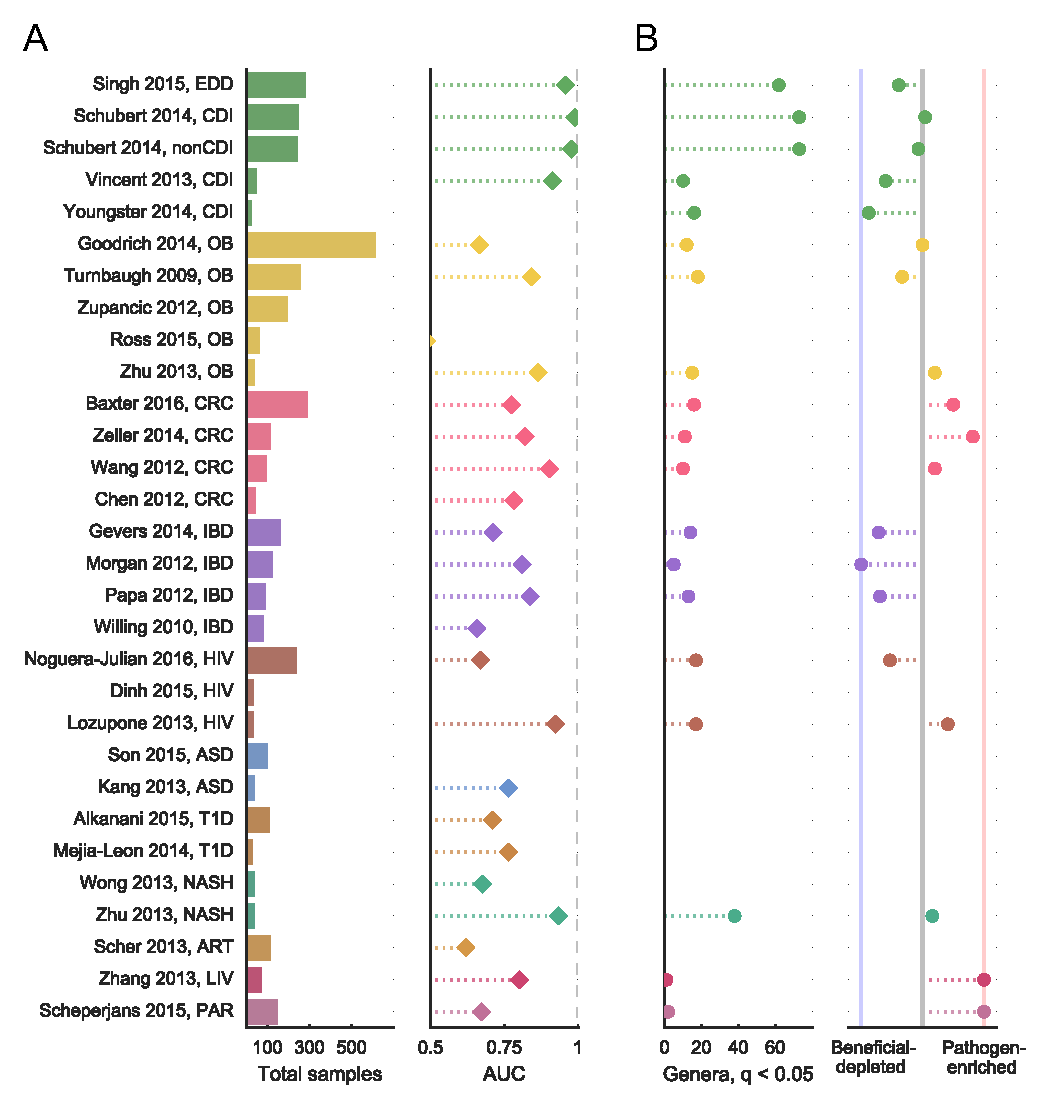
\includegraphics[width=1\textwidth]{samplesize_auc_nsig_balance.pdf}}
    \captionsetup{font=footnotesize,labelfont=footnotesize}
	\caption{\textbf{Most diseases show microbiome alterations, and consistent disease-associated shifts differ in their extent and direction.} (A) Left: Total sample size for each study included in these analyses. Additional information about each dataset can be found in Table \ref{tab:datasets}. Studies on the y-axis are grouped by disease and ordered by decreasing sample size (top to bottom). Right: Area under the ROC curve (AUC) for genus-level random forest classifiers. X-axis starts at 0.5, the expected value for a classifier which assigns labels randomly, and AUCs less than 0.5 are not shown. ROC curves for all datasets are in Supplementary Figure \ref{fig:roc_curves}. Note that Youngster et al. (2014) \cite{cdi-youngster} had only 4 distinct control patients was excluded from the Random Forest analysis. (B) Left: Number of genera with q $<$ 0.05 (Kruskal-Wallis (KW) test, Benjamini-Hochberg FDR correction) for each dataset. If a study has no significant associations, no point is shown. Right: Direction of the microbiome shift, i.e. the percent of total associated genera which were enriched in diseased patients. In datasets on the leftmost blue line, 100\% of associated (q $<$ 0.05, FDR KW test) genera are health-associated (i.e. depleted in patients relative to controls). In datasets on the rightmost red line, 100\% of associated (q $<$ 0.05, FDR KW test) genera are disease-associated (i.e. enriched in patients relative to controls). Supplementary Figures \ref{fig:overall_heatmap_qvalues} and \ref{fig:overall_heatmap_foldchange} show q-values and effects for each genus in each study.}
	\label{fig:fig1}
	\end{center}
\end{figure}

\newpage
\begin{figure}[h]
	\begin{center}
  	\makebox[\textwidth][c]{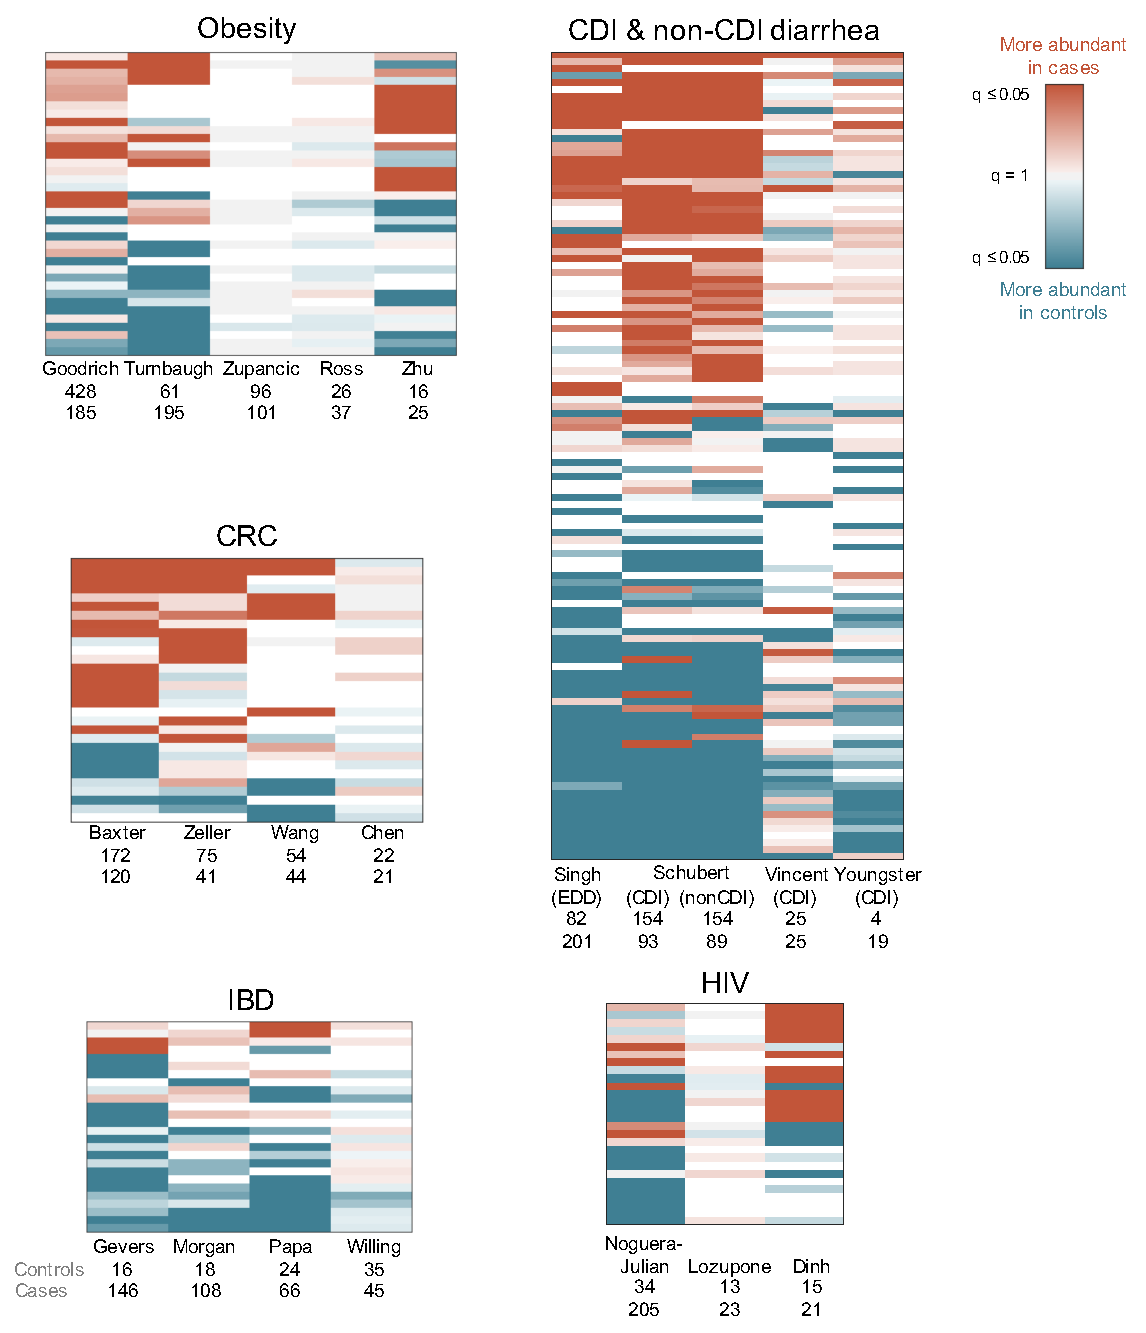
\includegraphics[width=0.9\textwidth]{disease_specific_heatmaps.pdf}}
    \captionsetup{font=footnotesize,labelfont=footnotesize}
	\caption{\textbf{Comparing results from multiple studies of the same disease reveals patterns in disease-associated microbiome alterations.} Heatmaps showing log10(q-values) for each disease (Kruskal-Wallis (KW) test, Benjamini-Hochberg FDR correction). Rows include all genera which were significant in at least one dataset within each disease, columns are datasets. Q-values are colored by direction of the effect, where red indicates higher mean abundance in disease patients and blue indicates higher mean abundance in controls. Opacity ranges from q = 0.05 to 1, where q values less than 0.05 are the most opaque and q values close to 1 are gray. White indicates that the genus was not present in that dataset. Within each heatmap, rows are ordered from most disease-associated (top) to most health-associated (bottom) (i.e. by the sum across rows of the log10(q-values), signed according to directionality of the effect). The extent of a disease-associated microbiome shift can be visualized by the number of rows in each disease heatmap; the directionality of a shift can be seen in the ratio of red rows to blue rows within each disease. See Supplementary Figure \ref{fig:supp_dis_specific} for genus (row) labels.}
	\label{fig:fig2}
	\end{center}
\end{figure}

\newpage
\begin{figure}[h]
	\begin{center}
  	\makebox[\textwidth][c]{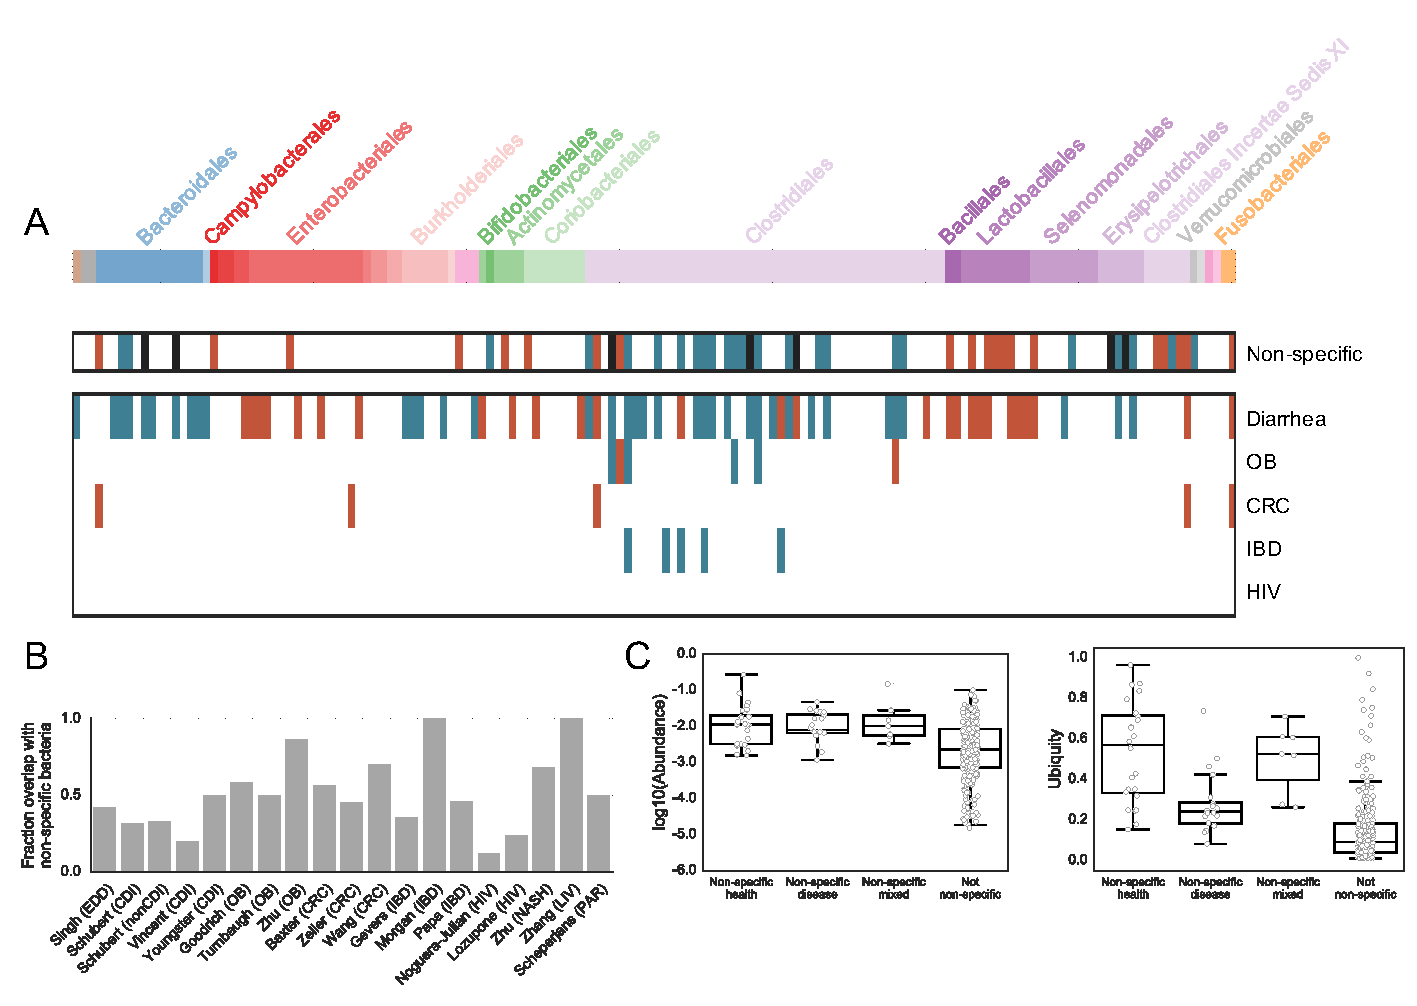
\includegraphics[width=\textwidth]{core_response.pdf}}
	\caption{\textbf{The majority of disease-associated microbiome alterations overlap with a non-specific microbial response to disease.} (A) Non-specific and disease-associated genera. Genera are in columns, arranged phylogenetically according to a PhyloT tree built from genus-level NCBI IDs (\url{http://phylot.biobyte.de}). Non-specific genera are associated with health (or disease) in at least two different \textit{diseases} (q $<$ 0.05, Kruskal-Wallis (KW) test, Benjamini-Hochberg FDR correction). Disease-specific genera are significant in the same direction in at least two \textit{studies} of the same disease (q $<$ 0.05, FDR KW test). As in Figure \ref{fig:fig2}, blue indicates higher mean abundance in controls and red indicates higher mean abundance in patients. Black bars indicate mixed genera which were associated with health in two diseases and also associated with disease in two diseases. Disease-specific genera are shown for diseases with at least 3 studies. Phyla, left to right: Euryarchaeota (brown), Verrucomicrobia Subdivision 5 (gray), Candidatus Saccharibacteria (gray), Bacteroidetes (blue), Proteobacteria (red), Synergistetes (pink), Actinobacteria (green), Firmicutes (purple), Verrucomicrobia (gray), Lentisphaerae (pink), Fusobacteria (orange). See Supplementary Figure \ref{fig:supp_meta_heatmap} for genus labels. (B) The percent of each study's genus-level associations which overlap with the shared response  (q $<$ 0.05, FDR KW test). Only datasets with at least one significant association are shown. (C) Overall abundance and ubiquity of non-specific genera across all patients in all datasets. Non-specific genera on the x-axis are as defined above.}
	\label{fig:fig3}
	\end{center}
\end{figure}

\bibliographystyle{unsrt}
\bibliography{meta-analysis/refs}


%% This is an example first chapter.  You should put chapter/appendix that you
%% write into a separate file, and add a line \include{yourfilename} to
%% main.tex, where `yourfilename.tex' is the name of the chapter/appendix file.
%% You can process specific files by typing their names in at the
%% \files=
%% prompt when you run the file main.tex through LaTeX.

%\graphicspath{{donor-selection/figures/}}

\chapter{Correcting for batch effects in case-control microbiome studies}

\noindent
Sean M Gibbons, Claire Duvallet, and Eric J Alm

\bigskip
\bigskip
\noindent
The contents of this chapter were published as: ``Correcting for batch effects in case-control microbiome studies'' in \textit{PLoS Computational Biology} (2018) volume 14(4), page e1006102.

\clearpage
%\section*{Abstract}

Early clinical successes are driving enthusiasm for fecal microbiota transplantation (FMT), the transfer of healthy gut bacteria through whole stool, as emerging research is linking the microbiome to many different diseases.
However, preliminary trials have yielded mixed results and suggest that heterogeneity in donor stool may play a role in patient response.
Thus, clinical trials may fail because an ineffective donor was chosen rather than because FMT is not appropriate for the indication.
Here, we describe a conceptual framework to guide rational donor selection to increase the likelihood that FMT clinical trials will succeed.
We argue that the mechanism by which the microbiome is hypothesized to be associated with a given indication should inform how donors are selected for FMT trials, categorizing these mechanisms into four disease models and presenting associated donor selection strategies.
We next walk through examples based on previously published FMT trials and ongoing investigations to illustrate how donor selection might occur in practice.
Finally, we show that typical FMT trials are not powered to discover individual taxa mediating patient responses, suggesting that clinicians should develop targeted hypotheses for retrospective analyses and design their clinical trials accordingly.
Moving forward, developing and applying novel clinical trial design methodologies like rational donor selection will be necessary to ensure that FMT successfully translates into clinical impact.


\newpage

\section{Introduction}

Fecal Microbiota Transplantation (FMT) is the transfer of gut bacteria through whole stool from a healthy donor to a recipient.
FMT has demonstrated high cure rates in C. difficile infection (CDI) across multiple randomized, placebo-controlled trials \cite{Quraishi2017} and has now entered standard of care for recurrent CDI in European and North American guidelines \cite{McDonald2018,Cammarota2017,Surawicz2013}.
Beyond CDI, FMT is being explored in range of microbiome mediated diseases, and has demonstrated promising results in inflammatory bowel disease \cite{Panchal2018,Gelfand2018,Kootte2017,Osman2018,Costello2017,Paramsothy2017}.

Despite these early successes, the underlying mechanism of FMT across all disease indications, including CDI, remains unclear.
However, it is generally considered that FMT restores gut microbial community perturbations from a dysbiotic to healthy stable state with engraftment of donor strains.
Other donor-dependent features may be important such as the abundance of non-bacterial components or donor clinical features \cite{Ott2017,Zuo2018}.
However, not all FMT donors are alike: gut microbiota compositions vary significantly within healthy populations in ways that could impact the findings from an FMT trial \cite{Yatsunenko2012}.
This critical point of donor microbiome variation is rarely considered in the development of FMT trials \cite{Bafeta2017,Olesen2018}.

Unlike FMT trials in CDI, where selecting donors based on specific clinical or microbiome profiles does not seem to affect clinical response rates, donor selection is likely to be crucial to trial outcomes in diseases with more complex host-microbiome interplay or distinct disease-associated perturbations.
Most notably, in a randomized controlled trial (RCT) of FMT for ulcerative colitis (UC) using 5 donors, 78\% of patients who achieved remission after FMT received stool from a single donor \cite{Moayyedi2015}.
Without this single donor the trial would have returned a negative result.
Given the variation in donor microbiomes and donors' potential impact on clinical efficacy, how should clinicians and investigators select their donors for a clinical trial?

To date, the typical approach for donor selection in FMT trials is to use a single healthy screened donor or to randomly select multiple donors from a set of screened potential donors \cite{Paramsothy2017,Kelly2016,vanNood2013}.
However, in clinical indications where successful donors may be rare, such as UC, clinical trials with randomly-selected donors may fail not because FMT is inappropriate for the indication, but because an ineffective donor was chosen.
An alternative approach is to expose patients to multiple donors in order to mitigate the risk of sub-optimal donor selection.
In a large RCT of FMT in UC, FMT enemas for a single patient were derived from between three and seven donors with patients receiving multiple donors throughout the 8 week course of treatment \cite{Paramsothy2017}.
However, using multiple donors for a single patient may not be feasible or appropriate in many disease indications or clinical trial settings (e.g. single-dose FMT studies).
Continuing the strategy of sub-optimal, random donor selection when it is not warranted risks returning false negative trials, stalling the field and delaying the development of novel therapies for seemingly intractable microbiome-mediated conditions.

Unlike traditional clinical trials which test well-defined small molecules, the therapy under study in FMT trials, the donor microbiome, also varies \cite{Olesen2018}.
Thus, translational FMT research requires a paradigm shift in order to systematically address rational donor selection.
Fortunately, with the emergence of large multi-donor stool banks, expanded access to genome sequencing technologies and publicly available microbiome sequencing datasets, rational donor selection is feasible and presents a unique opportunity to advance the research methods of this nascent field.

In this paper, we present a framework to guide donor selection for FMT trials.
The mechanism by which the microbiome is hypothesized to be associated with a given indication should inform how donors are selected for FMT trials, and we describe different disease models which may underlie microbiome-mediated conditions (Figure \ref{fig:disease-models}).
We describe strategies to rationally select donors for each type of disease model, and provide examples based on previously published FMT trials and ongoing investigations.
Finally, we discuss limitations of performing discovery-based retrospective research after an FMT clinical trial concludes.
To our knowledge, this is the first description of a comprehensive framework for rational donor selection in FMT trials.

\section{Models of microbiome-mediated disease}

FMT trials are pursued when research or clinical experiences suggest that a condition may be causally linked to the microbiome.
Here, we propose four different models which may underlie microbiome-mediated etiologies and their corresponding rational donor selection strategies (Figure \ref{fig:disease-models}).
Ultimately, it is up to each individual clinician-researcher to determine which of these model(s) are relevant in their specific case, based on published cross-sectional studies, mechanistic investigations in model organisms, and their own clinical experience treating patients.
Additionally, logistical considerations will be important factors in making the final donor selection regardless of which strategy is pursued.
Clinicians should ensure that the pool of donors that they are screening have enough material to sustain the required number of FMTs for their entire trial.

Most of the donor selection strategies described below can be modified to incorporate matching between patients and donors.
More specifically, donors can be tailored to individual patients to specifically make up for the unique taxonomic or functional deficiencies in that patient's microbiome.
With the increasing amount of microbiome data available from published FMT trials, we encourage collaborations between clinicians and bioinformaticians to analyze these data in order to generate or perhaps even confirm the validity of potential donor selection strategies before selecting one (Figure \ref{fig:ibd-butyrate}).
Finally, the strategies presented here should also be combined with adaptive clinical trial designs to further increase the probability of having a successful FMT trial \cite{Olesen2017}.

\begin{figure}
    \begin{center}
    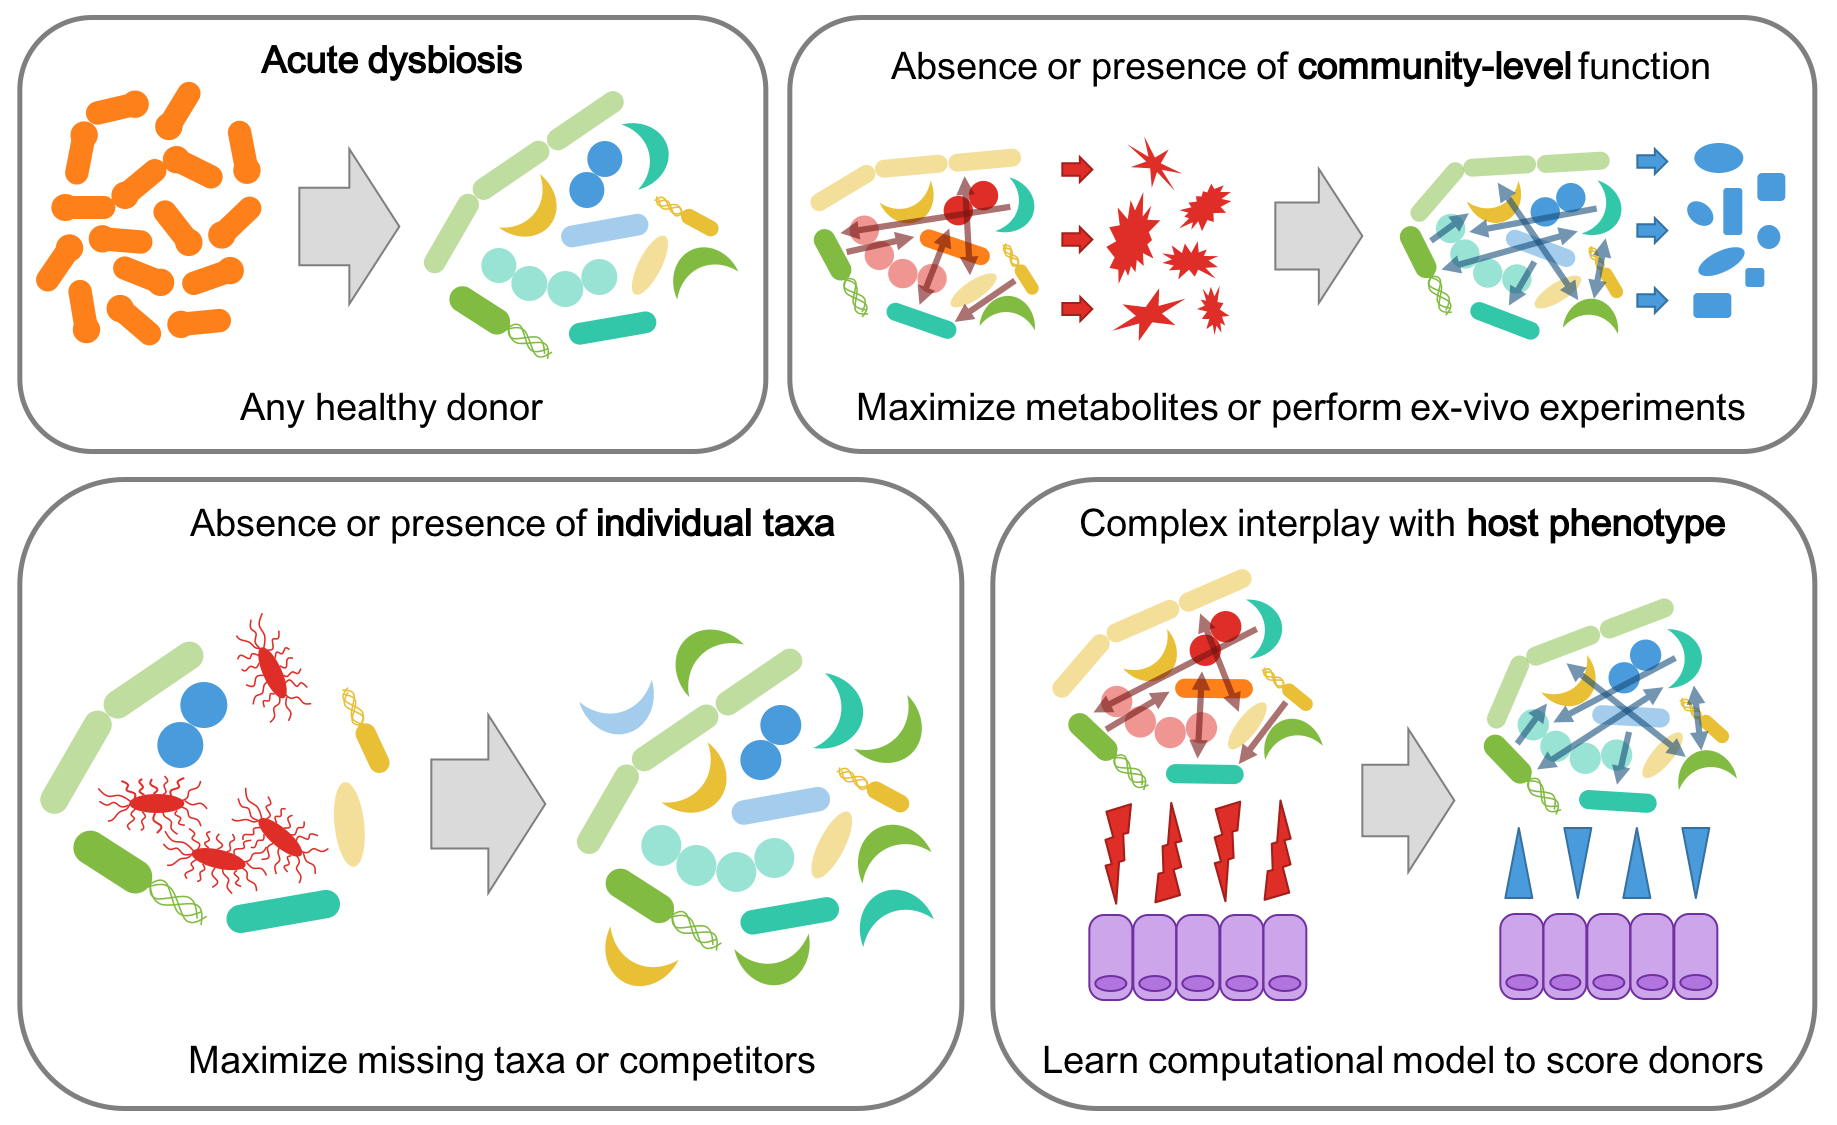
\includegraphics[width=\textwidth]{fig1_overview.png}
    \caption{Overview of the different models of microbiome-mediated disease and associated donor selection strategy.}\label{fig:disease-models}
    \end{center}
\end{figure}

\subsection{Acute dysbiosis}

An acutely dysbiotic gut microbial community is broadly dysfunctional and can no longer maintain the health of the host.
For example, in the case of recurrent Clostridium difficile infection, a disturbed microbial community is unable to prevent colonization by the pathogen, leading to recurrent overgrowth of C. diff and clinical symptoms \cite{Britton2014}.
Acute dysbiosis has also been described with the ``Anna Karenina principle'': all healthy microbiomes are alike but dysbiotic communities are all dysbiotic in their own ways \cite{Zaneveld2017}.
In this view of acute dysbiosis, microbial communities respond stochastically to stressors, resulting in dysbiotic communities which are characterized by increased variability rather than deterministic shifts to precise community type(s) \cite{Zaneveld2017}.

In this model, the host just needs to return to a ``healthy'' microbiome and thus choosing any healthy FMT donor should be sufficient to induce clinical improvements.
Because there is no specific disease-associated microbial community and deviation from health is instead the more important factor, simply replenishing the microbiome with a healthy configuration should be sufficient.
Indeed, FMT trials have demonstrated that recurrent C. diff infection can be effectively treated by almost any choice of donor \cite{Osman2016}.
In this case, researchers should consider how they define a ``healthy'' microbiome and how they will ensure engraftment of the transplanted healthy communities.

\subsection{Absence or presence of individual taxa}

\subsubsection{Absence of beneficial taxa}

In other cases, perhaps a disease is being caused or exacerbated by the lack of certain specific microbes, and replenishing these few taxa would be sufficient to restore the host to health.
For example, Hsiao et al showed that a single microbe, \textit{R. obeum}, restricted infection by \textit{V. cholerae} through quorum-sensing-mediated mechanisms \cite{Hsiao2014}.
Surprisingly, non-communicable diseases may also fall into this model: Wilck et al. demonstrated that a single strain of Lactobacillus was sufficient to prevent salt-induced hypertension, and follow-up studies indicate that similar mechanisms may be involved in salt-sensitive high blood pressure in humans as well \cite{Wilck2017}.

In these cases, the donor selection strategy should focus on maximizing the probability of engraftment of the beneficial taxa.
In cases where the unique taxa are not specifically known or are rare members of the human microbiota, many healthy donors should be pooled together to maximize the probability that the transplanted sample contains the necessary taxa.
If the missing microbes are known and well-characterized, on the other hand, researchers can screen their pool of potential donors to find the sample with the highest abundance of these taxa.

\subsubsection{Presence of harmful taxa}

Rather than being characterized by the absence of individual bacteria, perhaps a disease is instead mediated by the presence or overabundance of specific microbes, and removing these bacteria in a targeted fashion could lead to improvements in disease progression.
For example, \textit{Fusobacterium} has been found to be more abundant in colorectal cancer patients, specifically enriched in the tumors themselves \cite{Kostic2013}.
Multiple groups have identified mechanistic associations between \textit{Fusobacterium}, inflammatory transcriptional signatures, and tumor growth in mouse and human models of colorectal cancer, pointing to a causal role for \textit{Fusobacterium} in colorectal cancer progression \cite{Kostic2013,Rubinstein2013}.
Recent work has found that treating tumors with antibiotics slows tumor progression, further confirming these causal associations and pointing toward potential microbiome-based therapeutic interventions \cite{Bullman2017}.

Removing and replacing these bacteria should be the goal of FMT in cases where this disease model applies.
This can be achieved by first removing the harmful bacteria in a targeted way (e.g. via antibiotic treatment) with follow-up FMT to re-establish a healthy community that prevents their re-colonization.
In all cases, donors should be screened to exclude any samples which contain the harmful bacteria.
Donor samples can then be selected based on the abundance of bacteria which are known to out-compete the harmful taxa.
Competitors can be identified by searching the microbiology literature to identify bacteria which live in the same niche or which have been experimentally shown to directly out-compete the undesirable taxa, or they can perform these competition assays themselves.
If resources to perform competition assays are not available and the literature is sparse, researchers can also mine existing microbiome data to find bacteria which consistently anti-correlate with the harmful taxa, and choose donor samples with a high abundance of these putative competitors.

\subsubsection{Patient matching}

Taxa-based donor selection strategies are particularly amenable to patient-matching, when both patient and donor microbiome data are available prior to the start of a trial.
For example, if one patient is completely missing some of the beneficial taxa but not others, then these taxa can be weighted more heavily in the donor selection process.
The phylogenetic relationships between donor and recipient taxa could also be incorporated into donor selection: if a patient already has many bacteria which are closely phylogenetically related to known competitors of some of the harmful bacteria, then competitors of the other harmful bacteria can be upweighted in the donor selection process.
Similarly, if patients already have taxa which are already filling certain niches important for health, the taxa which fill those same niches can be downweighted in donor selection.

\subsubsection{Case study: Inflammatory Bowel Disease}

An example where the ``missing taxa'' model may be applicable is in inflammatory bowel disease (IBD).
Butyrate has long been associated with inflammatory bowel disease \cite{Scheppach1992}, and recent case-control and longitudinal studies point to a consistent lack of butyrate-producing bacteria in patients with IBD \cite{Duvallet2017,Schirmer2018}.
Furthermore, preliminary FMT trials in IBD have been marked by significant donor variability and suggest that donor microbiome characteristics may be associated with FMT response \cite{Moayyedi2015,Kump2018}.
These results indicate that IBD may benefit from rational donor selection approach, and that donors with high abundances of butyrate-producing organisms may yield higher FMT response rates than randomly selected donors.

Given the availability of microbiome data from completed FMT studies, we tested this hypothesis that IBD trials would benefit from a rational donor selection strategy based on the ``absence of beneficial taxa'' disease model.
We re-analyzed microbiome data from three completed IBD FMT trials which provided publicly available sequencing data for patient and donor samples \cite{Kump2018,Goyal2018,Jacob2017}.
We selected butyrate-producers based on their genus-level taxonomy, using the genera identified in Vital et al. 2017 (see Methods, \cite{Vital2017}).
Donors in the three studies exhibited a range of total abundances of butyrate-producing bacteria (Figure \ref{fig:ibd-butyrate}A).
Surprisingly, however, the abundance of butyrate producers in the donor stool was not associated with recipient patients' clinical responses (Figure \ref{fig:ibd-butyrate}B).
We also found no association with response when matching donor abundances with their respective patient's original abundance of butyrate producers (Supplementary Figure \ref{fig:delta-butyrate}).
These results show that selecting donors based on the abundance of butyrate producers may not yield improved clinical trial outcomes in IBD, and illustrates the process by which clinicians could approach and validate a rational donor selection strategy based on individual taxa.
More complex methods to identify butyrate producers (e.g. using phylogenetic-aware methods and/or metagenomics data) could be used in the next iteration to develop a donor selection strategy, if these data are available to clinicians.
Another approach, discussed below, is to select donors based on functional community assays and direct measurement of butyrate production rather than microbial taxonomies alone.

\begin{figure}
    \begin{center}
    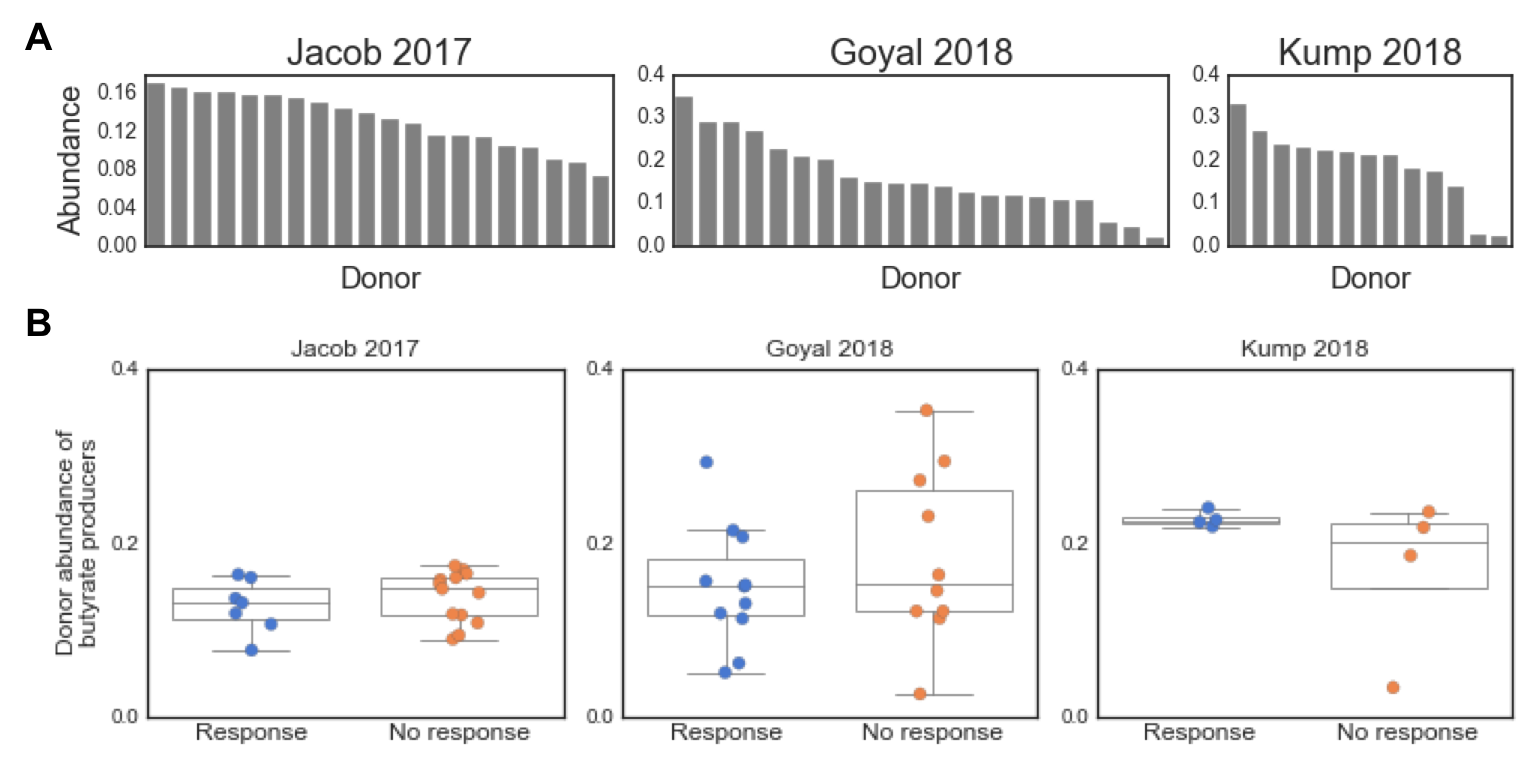
\includegraphics[width=\textwidth]{fig2_ibd_butyrate.png}
    \caption{Case study in IBD: select donors based on abundance of butyrate producers? (A) abundance of butyrate producers in each study's donor samples. (B) abundance of butyrate producers in donor samples, stratified by respective patient's response.}\label{fig:ibd-butyrate}
    \end{center}
\end{figure}

\subsection{Community-level functionality}

Some microbiome-associated diseases may not be addressable by replenishing the patient with a generically healthy community or by targeting individual taxa, and may instead be mediated by the microbiome through a community-level function.
Here, there may not be a consistent disease-associated microbiome across patients in terms of taxonomic composition, but patients may be characterized by having microbiomes which are similarly missing or enriched in some core functionality.
This model may also apply to conditions where there are consistent disease- or health-associated taxa, but in which their collective functioning is the more important mediator of disease.
The IBD case study described above may reflect this situation: although depletion of butyrate producers is strongly associated with IBD throughout the literature, a successful donor selection strategy may need to consider butyrate production directly rather than through the proxy of taxonomy \cite{Duvallet2017,Schirmer2018}.

\subsubsection{Missing community-level function}

In the case where a community-level function is missing from patients' microbiomes, the goal of FMT should be to replace the deficient community with a beneficially functional microbiome.
Here, it is important that a single donor with an intact microbial community is used, rather than a mixture of donors which may not yield the desirable community composition at steady-state after engraftment.
To choose a donor, molecules which can serve as proxies for the metabolic output of the microbial community can be measured directly in donor stool, and donors can be selected based on the abundance of these molecules.

Like IBD, hepatic encephalopathy (HE) is an example where community functionality is likely more relevant to FMT outcome than specific taxa.
A previous trial in HE \cite{Bajaj2017} rationally selected their single donor by maximizing the abundance of \textit{Lachnospiraceae} and \textit{Ruminococcaceae}, taxa which were identified based on cross-sectional microbiome data.
The clinical trial was a success, but it remains unclear from this trial whether the donor's strains engrafted in the patients post-FMT and whether this played any role in the successful FMT responses.
The exact mechanisms of action of these strains remains unknown, though both bacterial families are known short chain fatty acid producers (in particular butyrate) \cite{Vital2017}.
More recent studies have more directly implicated the production of short chain fatty acids and secondary bile acids as being important in liver cirrhosis and subsequent complications such as HE, suggesting that community-level functioning may be a more important driver of FMT response.
Thus, HE may be a case in which function-based donor selection can be employed.

To illustrate this process, we analyzed stool metabolomics data from 83 OpenBiome donors and used this data to rank them based on their estimated production of short chain fatty acids and secondary bile acids (Figure \ref{fig:bn10-liver}).
As in the IBD case study, we found that donors exhibited a range of values for our metabolites of interest (Figure \ref{fig:bn10-liver}A and C).
We ranked donors based on their amounts of the three measured short-chain fatty acids (butyrate, isovalerate, and propionate) and on their bile acid conversion rates, approximated as the ratio between the total amounts of primary and secondary bile acids (Figure \ref{fig:bn10-liver}B and D).
With this process, we were able to identify four donors who were in the top 25\% of all donors for both metrics (Figure \ref{fig:bn10-liver}E).
In a real FMT trial, a clinician would then work with their stool bank to ensure that these donors were still active and/or had enough material to be used in the full trial.

While measuring metabolites in stool as a proxy for community production will likely be an improvement over taxonomy-based approaches in most cases, these measurements are also complicated by potential host effects.
For example, different hosts may absorb these molecules at different rates, and so measuring them in stool may not be an accurate reflection of each donor community's productive potential.
Additionally, community function may depend on non-biologically relevant factors like the donor's diet and time that they provided their sample. As an example, bile acid production spikes after meals \cite{Hofmann1989}, so the amount of bile acids measured in a given stool sample may reflect the amount of time since the donor last ate rather than their actual microbial community's functional production of these molecules.
If clinicians have access to sufficient resources, a better way to screen donors may be to perform ex-vivo assays, in which each donor sample is homogenized and provided with the substrates (e.g. fiber) needed to produce the desirable output (e.g. short-chain fatty acids like butyrate).
In this way, the donor community function can be measured directly \cite{Wang1993,Chen2017}.

\begin{figure}
    \begin{center}
    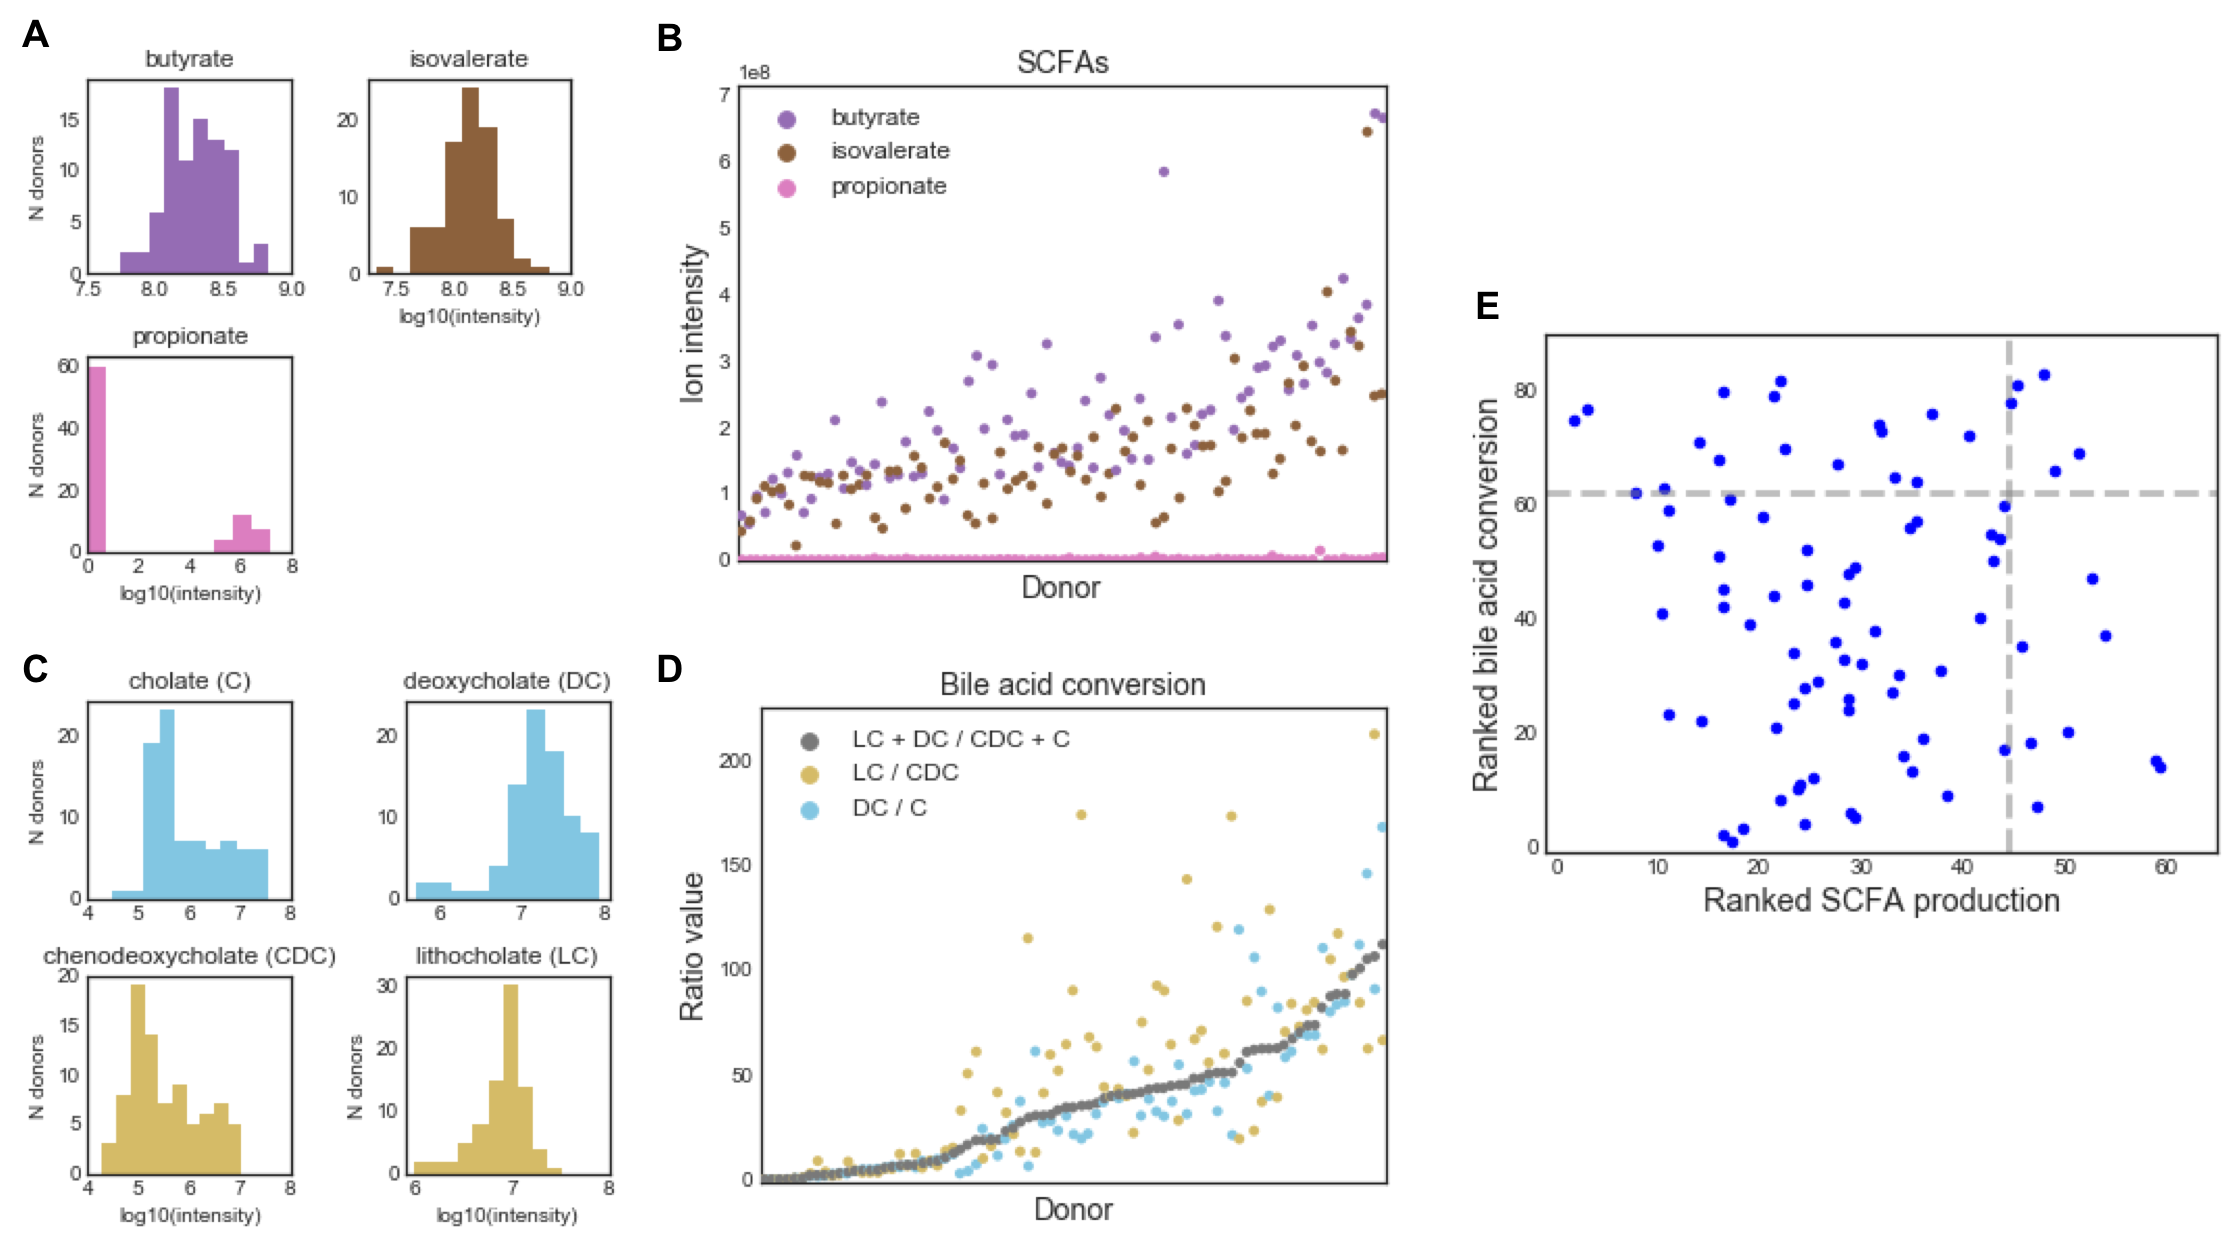
\includegraphics[width=\textwidth]{fig3_cirrhosis_metabolomics.png}
    \caption{Case study in liver cirrhosis: selecting donors based on community function by mining stool metabolomics data. (A) Distribution of SCFAs in all donor stools. (B) Abundance of each SCFA per donor, ranked by average SCFA abundance. (C) Distribution of bile acids in all donors. Primary bile acids are in the left column, secondary bile acids are in the right column. Bile acids are colored according to pathways. (D) Bile acid conversion ratios in each donor, ranked by total secondary to primary bile acids. (E) The five donors in the top 25\% for both of these metrics, for example, could be used in a rationally-designed liver cirrhosis FMT trial.}\label{fig:bn10-liver}
    \end{center}
\end{figure}

\subsubsection{Overactive function}

A disease may also be mediated by an overactive microbiome doing something harmful to the host.
For example, many studies have shown a causal association between TMAO produced by the microbiota and atherosclerosis \cite{Koeth2013,Wang2015}.
Here, the goal of FMT should also be to replace the patient's microbiome with a beneficially functional community, but the donor selection strategy may attempt to identify communities in which the harmful function is completely absent or which produces an inhibitor of the harmful microbe-derived molecule \cite{Wang2015}.

\subsection{Microbiome-associated host phenotypes}

Diseases with more complex etiologies may not have a direct taxonomic or functional association with the microbiome but instead be related through some intermediate host phenotype which needs to be improved or corrected.
For example, severe acute malnutrition has been associated with a gut microbiota which is not fully mature, with mouse experiments suggesting that this association may be causal \cite{Blanton2016,Subramanian2014}.
Other studies have shown a relationship between gut microbiome, immune development, and development of autoimmune conditions later in life \cite{Stokholm2018,Cox2014,Kostic2015}.
These relationships may have mechanistic explanations which are not directly measurable from donor or patient stool (e.g. immunogenicity of bacteria, ability of bacteria to eat the host's mucus, etc) but which can nevertheless be inferred from existing data and used to select potential donors.

For these more complex cases, models can be trained from existing datasets to learn the community signatures linked to the disease-associated phenotype. In some cases, it may be possible to develop computational models which directly predict the phenotype of interest.
For example, Stein et al. developed a model to predict the induction of regulatory T-cells by microbial communities \cite{Stein2018}.
In other cases with few known mechanistic models, machine learning algorithms can be trained on multiple cross-sectional datasets to identify complex signatures that reproducibly distinguish patients from healthy controls.
These models can then be applied to score potential donors, and the donor with the ``most healthy'' score may be chosen for a trial.

\section{Little understanding of underlying disease model}

In some conditions, there may not be enough understanding of the underlying microbiome-based etiology to inform donor selection in an FMT trial. It may also be the case that there are no existing datasets on which to train models, existing datasets are not sufficiently powered to distinguish the different potential underlying models, or logistical considerations constrain a clinician's ability to select specific donors for their trial. In these cases, we recommend selecting different healthy donors, employing an adaptive clinical trial design in which donors are cycled after they have clinical failures (as described previously in \cite{Olesen2017}), and performing retrospective analyses to answer targeted hypotheses which were developed during the clinical trial design process.

\subsection{Cycling healthy donors in adaptive trials}

As donors change through the course of an adaptive trial, clinicians may elect to select their donors randomly or to more rationally cycle through donors \cite{Olesen2017}.
``Differently healthy'' donors may be selected, perhaps representing different underlying disease-associated models described above.
Donors may also be selected to span the range of ``healthy'' microbiomes in a given population.
For example, clinicians may pick a ``median'' health donor (i.e. one who is about as similar to all reference microbiomes), define a ``healthy plane'' and pick donors based on their distance to this plane (as in \cite{Halfvarson2017}), or simply based on the presence or abundance of certain consistently ``core'' health-associated bacteria \cite{Shade2011},\cite{Duvallet2017}.
In a similar vein, ``healthy'' donors can also be chosen based on their distance from disease-associated microbiomes, as opposed or in addition to similarity to health. Published case-control datasets can be used to identify donors with communities which are farthest away from the median or average diseased patient.
These datasets can also be mined to identify taxa which are consistently disease-associated, and which should be minimized or perhaps even absent in the potential donor.
Pairing rational donor selection with adaptive trial designs may eventually yield insight into the underlying model mediating the disease of interest if certain types of ``healthy'' donors consistently perform better at treating patients than others.

\subsection{Discovery-based retrospective analyses}

In these exploratory FMT clinical trials, discovering microbiome characteristics which are differentially associated with FMT response may be a valuable secondary endpoint \cite{Olesen2018}, identifying characteristics of good donors and informing donor selection strategy for future trials.
Furthermore, companies attempting to develop microbiome-based therapeutics may use FMT trials to discover the key bacteria which mediate FMT response in order to include these in their microbial cocktail product.
However, exploratory FMT trials tend to enroll few patients, limiting the potential power of retrospective analyses to find associations between the microbiome and FMT response.

We performed a simulation to determine the likelihood of a retrospective analysis to identify donor-derived bacteria associated with different patient responses to FMT.
We performed this simulation for multiple FMT trial set-ups and outcomes (i.e. number of FMT responders and non-responders).
We used existing microbiome datasets to model different effect sizes, where we use ``effect size'' to mean the number of bacteria which are differentially abundant in donor samples given to patients who did and did not respond to FMT.
We used case-control datasets to model the microbiome data and various effect sizes, with a large effect represented by an infectious diarrhea dataset \cite{Schubert2014}, a medium effect represented by colorectal cancer \cite{Baxter2016}, and a weak effect represented by obesity \cite{Goodrich2014}.
For each of these datasets, we identified the top ten most differentially abundant bacteria in the overall population as the key mediating bacteria (see Methods).
Next, we simulated different trials, varying the numbers of patients in the FMT arm and the FMT response rates (i.e. proportion of patients which were FMT responders, represented by sampling from the ``case'' patients, vs. non-responders, represented by sampling from the ``control'' patients, representing non-responders).
We subsampled patients according to these parameter settings, identified differentially abundant genera, and compared these to the top ten genera identified from the entire datasets (Figure \ref{fig:power-sim}).

In cases where the microbial signature for FMT response is expected to be large (i.e. the difference in donor stools given to FMT responders vs. non-responders is as large as the effect of diarrhea effect on the microbiome), we found that small FMT trials would recover most of the top hits in most cases.
The power to detect associations decreased as FMT response rates became less balanced (i.e. response rates different from 50\%), and in these cases trials would need to include up to 50 patients in the FMT arm to recover the key mediating taxa.
For both medium and small effect sizes, however, prohibitively large FMT arms would be needed to recover most key mediating taxa.
We found that when the microbial signature for FMT is equivalent to the effect of diseases like colorectal cancer on the microbiome, at least 100 patients are needed in the FMT arm to recover at least half of the most truly differentially abundant genera for most FMT trials.

These results suggest that successful secondary analyses of microbiome data from FMT trials will require either very large FMT arms, investigating more targeted hypotheses, or additional sample collections.
For example, clinicians may consider pairing donor and patient samples or collecting longitudinal patient samples to increase power to make discoveries.
They may also consider testing specific hypotheses developed before the trial, such as comparing the total abundance of butyrate producers between FMT responders and non-responders, or performing functional assays to measure specific metabolites thought to be associated with FMT response.
On the other hand, researchers wishing to identify the key taxa to include in an FMT drug may consider pursuing clinical trials in which identifying these taxa is the primary endpoint, and power them accordingly.


\begin{figure}
    \begin{center}
    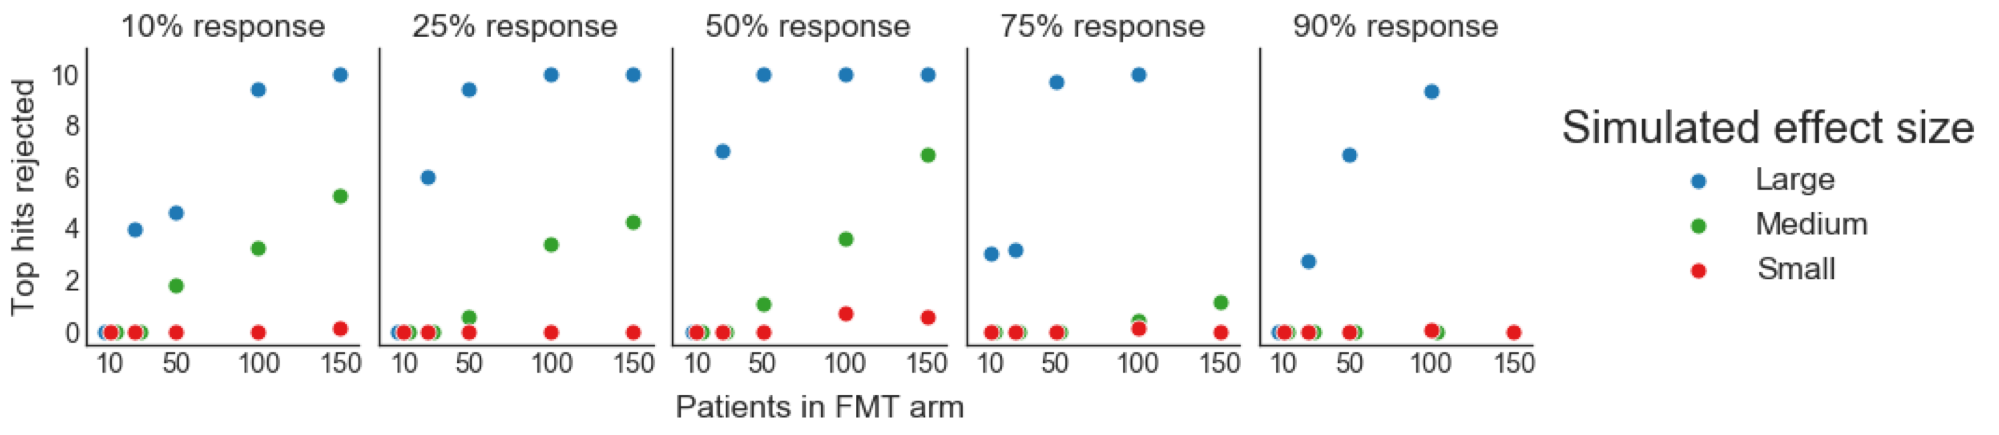
\includegraphics[width=\textwidth]{fig4_power_simulation.png}
    \caption{Power simulation results, showing how many of the 10 most ``truly'' differentially abundant genera would be recovered as significant under different FMT study designs. Each panel represents a different FMT response rate (i.e. percent of patients in the responder vs. non-responder group). The effect size (i.e. number of genera which are differentially abundant in FMT responders vs. non-responders) was simulated by using three different case-control microbiome datasets. A large effect size is modeled by the effect of diarrhea on the microbiome, medium by colorectal cancer, and small by obesity. The top 10 "true" differentially abundant genera were identified by calculating their signal-to-noise ratios in the full original dataset (i.e. mean difference divided by the standard deviation).}\label{fig:power-sim}
    \end{center}
\end{figure}

\section{Discussion}

The framework presented here encourages clinicians to leverage their clinical experience, existing microbiome research and published datasets, and the increasing availability of screened donor stools to more efficiently translate microbiome-based interventions into clinical impact.
Clinicians can apply their existing knowledge and a priori hypotheses to determine which microbiome-mediated disease model may underlie their indication of interest, and then select donors accordingly.
By rationally choosing donors during the FMT trial design, clinicians will increase the likelihood of successful FMT trials in diseases in which donor heterogeneity affects patient response.
Our power simulation analysis also suggests that specific plans for retrospective analyses of the microbiome data generated should be developed during trial design, with targeted hypotheses of interest and sample collection plans tailored accordingly.
Otherwise, exploratory analyses are unlikely to make new discoveries from most FMT trials. Paired with adaptive clinical trial designs, FMT trials with rationally-selected donors will become an important tool in advancing translational microbiome research and clinical treatment to improve and save patient lives.

As clinical trial design methodologies for FMT trials become more developed, many additional questions will need to be addressed.
Many of these key questions relate to the nuances involved in choosing healthy donors: what defines a ``healthy'' donor, and what should define one?
These questions are critical because regardless of the underlying model, in all cases a healthy donor must be identified.
However, as our understanding of the microbiome in societies around the world continues to increase, consensus on the exact structure of a ``healthy'' microbiome decreases.
Should donors be selected to reflect the patient populations, or simply be devoid of pathogens and source from as ``healthy'' of donors as possible?
We know that Europeans and North Americans tend to have less \textit{Prevotella} than healthy Africans from across the continent in both urban and rural communities \cite{Yatsunenko2012,Ou2013,DeFilippo2010}.
Thus, should a clinician carrying out an FMT trial in an African setting use local African cohort as their donor population in order to better match the expected ``healthy'' state of their participants?
In some cases, using a local population may be incompatible with established donor screening criteria because of geographical differences in baseline microbial community composition, prior likelihood of pathogen colonization, or differences in diet and lifestyle habits leading to different dominating strains.
Should clinicians consider relaxing donor screening and exclusion criteria in cases where donors are sourced from countries where commensal colonization by potential pathogens is common population-wide?
More research to understand the functional differences and clinical implications of different ``healthy'' communities across global populations and specifically in the context of FMT trials will be required before these and many related questions can be answered \cite{Bello2018,Rabesandratana2018}.

On the patient side, comorbidities, lifestyle, and dynamic disease manifestations may present challenges and opportunities to improve donor selection processes.
How should comorbidities be incorporated into donor selection?
Patients with multiple disease processes may be dominated by one microbiome-mediated disease model or may exhibit a combination of models, perhaps affecting which donors would be optimal for their specific case.
For example, a person with one community-level function process and one acute dysbiosis process may respond well to total community replacement alone, or may require a combination of total community replacement along with enrichment for community function.
Additionally, will diseases that change manifestations over time benefit from employing different donor selection strategies over the course of a longitudinal FMT trial?
Although there have been no serious adverse events related to FMT material in either clinical practice for rCDI or in clinical trials across adults or pediatrics, could some donors further reduce the probability of adverse events in at-risk patients?
Finally, how should other sources of heterogeneity like lifestyle, diet, and medication usage be incorporated into rational donor selection?
In cases where FMT is combined with other microbiome-targeted interventions like prebiotics or dietary changes, could some donors have synergistic effects with these paired interventions and lead to greater clinical success?

To ensure that FMT reaches its full potential to improve and save patient lives, clinicians should think critically about how their FMT trials can be designed for maximal impact.
By applying new approaches like rational donor selection and adaptive trial designs, the number of trials which fail even though they could have succeeded will drastically decrease.
Furthermore, by developing targeted hypotheses, post-trial analysis plans, and associated sample collection schema alongside the core FMT trial design itself, the number of basic scientific discoveries that are made from each trial will significantly increase.
As FMT expands far beyond rCDI and microbiome-based therapeutics are developed to target a range of disease, novel methods and approaches tailored to the unique challenges and opportunities presented by FMT will be critical to ensuring the advancement of translational microbiome science and beneficial impact on patient lives.

\section{Methods}

\subsection{Microbiome data processing}

Raw fastq data files were downloaded from the European Nucleotide Archive using the following accession numbers: Jacob et al 2017, PRJNA388210; Goyal et al. 2018, PRJNA380944; and Kump et al. 2018, PRJEB11841.
All data was processed using QIIME 2 (v. 2018.6.0, \cite{qiime2}).
Briefly, data was imported into QIIME 2 as paired-end (Kump et al. 2018; Jacob et al. 2017) or single-end (Goyal et al. 2018) data, filtered based on sequence quality with \texttt{quality-filter q-score}, and denoised with deblur using \texttt{deblur denoise-16S} \cite{deblur}.
Representative sequences were assigned taxonomy using \texttt{feature-classifier classify-sklearn} with the GreenGenes-trained Naive Bayes classifier provided by QIIME 2 (gg-13-8-99-nb-classifier.qza) \cite{feature-classifier}.
All data was exported to tab-delimited format and analyzed in Python 2.7.6.

\subsection{Quantifying abundance of butyrate producers}

We identified butyrate producers at the genus-level based on the analysis performed in Vital et al. 2017 \cite{Vital2017}.
These taxa were detected in >70\% of individuals in Vital et al. 2017, are known butyrate producers (with a majority of the analyzed representative genomes containing known butyrate production pathways), and accounted for the majority of the total butyrate pathway abundances in human metagenomics data.
We removed \textit{E. ventriosum}, \textit{E. hallii}, and \textit{E. rectale} from our analyses as these species-level taxa do not comprise one genus with conserved butyrate production.

\subsection{Stool metabolomics}

Metabolomics data was generated as described in Poyet, Groussin, Gibbons et al. (in preparation) and downloaded after personal communication with the authors.
For donors with multiple samples, we considered the mean metabolite abundances across all sampled time points.
We identified three short chain fatty acids in the data (propionate, butyrate, and isovalerate) and the major primary (cholate and chenodeoxycholate) and secondary (deoxycholate and lithocholate) bile acids.
Lithocholate was available for both C-18 negative and HILIC negative modes; we considered only the C-18 negative data to match the other bile acids.
Bile acid conversion rates were calculated as in Kakiyama et al. 2013 \cite{Kakiyama2013}.
Donors were ranked based on their average SCFA abundances and based on the total bile acid conversion ratio ( (lithocholate + deoxycholate) / (chenodeoxycholate + cholate) ).

\subsection{Power simulation}

We performed a simulation to determine the power of FMT trials to retrospectively find associations between donor bacterial abundances and FMT response.
We used case-control gut microbiome datasets from MicrobiomeHD \cite{Duvallet2017} to model different effect sizes for FMT response.
Here, we use ``effect size'' to mean the number of genera which are differentially abundant between patients who respond to FMT vs. patients who do not.
Per the results in MicrobiomeHD, we used infectious diarrhea to model a large effect \cite{Schubert2014}, colorectal cancer to model a medium effect \cite{Baxter2016}, and obesity to model a small effect \cite{Goodrich2014}.
We collapsed OTUs to genus-level as in \cite{Duvallet2017} and ranked genera according to their signal-to-noise ratio in each entire dataset, where the signal-to-noise was calculated as the difference in mean log abundance in cases and controls divided by the standard deviation of the log abundances across all samples.
We considered the 10 genera with the largest absolute signal-to-noise ratios as our ``top hits'' in the main text.

We modeled different FMT clinical trial designs and outcomes by varying the number of total patients in the trial and the percent of FMT responders (i.e. the number of patients we selected from the original ``case'' group relative to the original ``control'' patients, to model FMT responders and non-responders).
For each of these designs, we subsampled the correct number of case samples to represent FMT responders and control samples to represent non-responders from the original datasets.
We identified significantly differentially abundant genera with the \texttt{kruskalwallis} function from \texttt{scipy.stats.mstats} (scipy v. 1.1.0) as genera with q $<$ 0.05 after multiple hypothesis testing correction with the \texttt{multipletests} function (\texttt{method=`fdr\_bh'}) from the \texttt{statsmodels.sandbox.stats.multicomp} package (statsmodels v. 0.9.0).
We then counted how many of the top genera identified through the signal-to-noise ranking were identified as significantly different as a proxy for the power to detect effects.

\subsection{Code and data availability}

Code to reproduce all of these analyses and figures can be found at \url{https://github.com/cduvallet/donor-selection/}.
Data were downloaded from original sources as described above.

\newpage
\section{Supplementary Figure}

\FloatBarrier
\begin{figure}[h]
    \begin{center}
    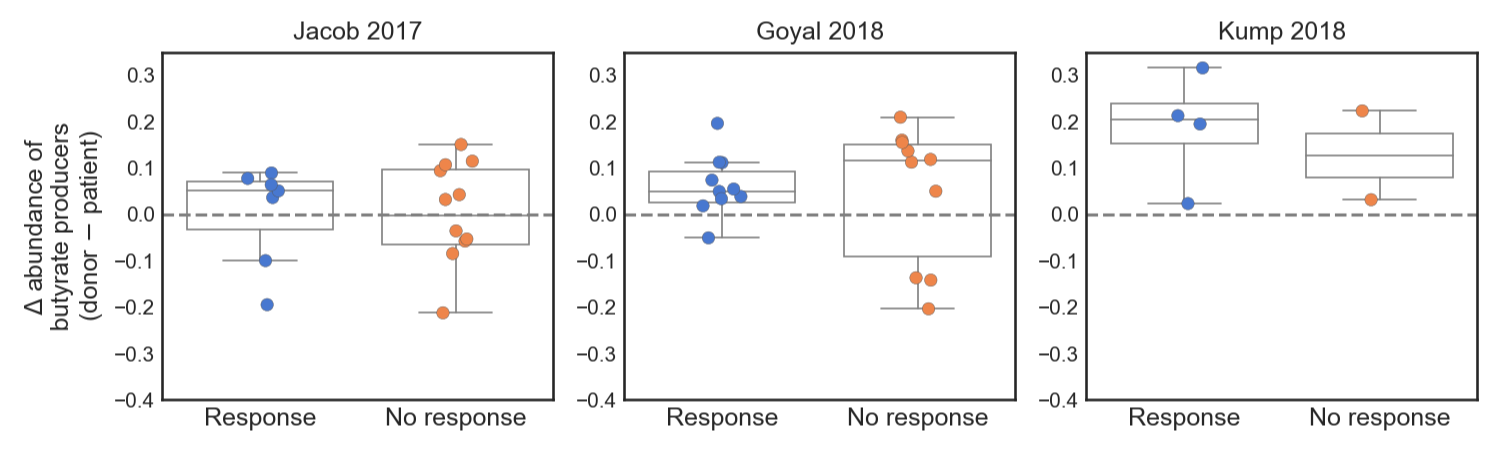
\includegraphics[width=\textwidth]{suppfig_delta_butyrate_vs_response.png}
    \caption{Difference between abundance of butyrate producers in donor sample and respective patient sample, stratified by patient response.}\label{fig:delta-butyrate}
    \end{center}
\end{figure}

\begin{singlespace}
\bibliographystyle{unsrtnat}
\bibliography{donor-selection/donor-selection-refs.bib}
\end{singlespace}


%% This is an example first chapter.  You should put chapter/appendix that you
%% write into a separate file, and add a line \include{yourfilename} to
%% main.tex, where `yourfilename.tex' is the name of the chapter/appendix file.
%% You can process specific files by typing their names in at the
%% \files=
%% prompt when you run the file main.tex through LaTeX.

\graphicspath{{donor-selection/figures/}}

\chapter{Increasing fecal microbiota transplant clinical trial successes by applying rational donor selection}\label{chap:donor-selection}

\noindent
Claire Duvallet, Caroline Zellmer, Pratik Panchal, Shrish Budree, Majdi Osman, and Eric J Alm.

\bigskip
\bigskip
\noindent
The contents of this chapter constitute a manuscript in preparation for submission.

\clearpage
\section*{Abstract}

Early clinical successes are driving enthusiasm for fecal microbiota transplantation (FMT), the transfer of healthy gut bacteria through whole stool, as emerging research is linking the microbiome to many different diseases.
However, preliminary trials have yielded mixed results and suggest that heterogeneity in donor stool may play a role in patient response.
Thus, clinical trials may fail because an ineffective donor was chosen rather than because FMT is not appropriate for the indication.
Here, we describe a conceptual framework to guide rational donor selection to increase the likelihood that FMT clinical trials will succeed.
We argue that the mechanism by which the microbiome is hypothesized to be associated with a given indication should inform how donors are selected for FMT trials, categorizing these mechanisms into four disease models and presenting associated donor selection strategies.
We next walk through examples based on previously published FMT trials and ongoing investigations to illustrate how donor selection might occur in practice.
Finally, we show that typical FMT trials are not powered to discover individual taxa mediating patient responses, suggesting that clinicians should develop targeted hypotheses for retrospective analyses and design their clinical trials accordingly.
Moving forward, developing and applying novel clinical trial design methodologies like rational donor selection will be necessary to ensure that FMT successfully translates into clinical impact.


\newpage

\section{Introduction}

Fecal Microbiota Transplantation (FMT) is the transfer of gut bacteria through whole stool from a healthy donor to a recipient.
FMT has demonstrated high cure rates in C. difficile infection (CDI) across multiple randomized, placebo-controlled trials \cite{Quraishi2017} and has now entered standard of care for recurrent CDI in European and North American guidelines \cite{McDonald2018,Cammarota2017,Surawicz2013}.
Beyond CDI, FMT is being explored in range of microbiome mediated diseases, and has demonstrated promising results in inflammatory bowel disease \cite{Panchal2018,Gelfand2018,Kootte2017,Osman2018,Costello2017,Paramsothy2017}.

Despite these early successes, the underlying mechanism of FMT across all disease indications, including CDI, remains unclear.
However, it is generally considered that FMT restores gut microbial community perturbations from a dysbiotic to healthy stable state with engraftment of donor strains.
Other donor-dependent features may be important such as the abundance of non-bacterial components or donor clinical features \cite{Ott2017,Zuo2018}.
However, not all FMT donors are alike: gut microbiota compositions vary significantly within healthy populations in ways that could impact the findings from an FMT trial \cite{Yatsunenko2012}.
This critical point of donor microbiome variation is rarely considered in the development of FMT trials \cite{Bafeta2017,Olesen2018}.

Unlike FMT trials in CDI, where selecting donors based on specific clinical or microbiome profiles does not seem to affect clinical response rates, donor selection is likely to be crucial to trial outcomes in diseases with more complex host-microbiome interplay or distinct disease-associated perturbations.
Most notably, in a randomized controlled trial (RCT) of FMT for ulcerative colitis (UC) using 5 donors, 78\% of patients who achieved remission after FMT received stool from a single donor \cite{Moayyedi2015}.
Without this single donor the trial would have returned a negative result.
Given the variation in donor microbiomes and donors' potential impact on clinical efficacy, how should clinicians and investigators select their donors for a clinical trial?

To date, the typical approach for donor selection in FMT trials is to use a single healthy screened donor or to randomly select multiple donors from a set of screened potential donors \cite{Paramsothy2017,Kelly2016,vanNood2013}.
However, in clinical indications where successful donors may be rare, such as UC, clinical trials with randomly-selected donors may fail not because FMT is inappropriate for the indication, but because an ineffective donor was chosen.
An alternative approach is to expose patients to multiple donors in order to mitigate the risk of sub-optimal donor selection.
In a large RCT of FMT in UC, FMT enemas for a single patient were derived from between three and seven donors with patients receiving multiple donors throughout the 8 week course of treatment \cite{Paramsothy2017}.
However, using multiple donors for a single patient may not be feasible or appropriate in many disease indications or clinical trial settings (e.g. single-dose FMT studies).
Continuing the strategy of sub-optimal, random donor selection when it is not warranted risks returning false negative trials, stalling the field and delaying the development of novel therapies for seemingly intractable microbiome-mediated conditions.

Unlike traditional clinical trials which test well-defined small molecules, the therapy under study in FMT trials, the donor microbiome, also varies \cite{Olesen2018}.
Thus, translational FMT research requires a paradigm shift in order to systematically address rational donor selection.
Fortunately, with the emergence of large multi-donor stool banks, expanded access to genome sequencing technologies and publicly available microbiome sequencing datasets, rational donor selection is feasible and presents a unique opportunity to advance the research methods of this nascent field.

In this paper, we present a framework to guide donor selection for FMT trials.
The mechanism by which the microbiome is hypothesized to be associated with a given indication should inform how donors are selected for FMT trials, and we describe different disease models which may underlie microbiome-mediated conditions (Figure \ref{fig:disease-models}).
We describe strategies to rationally select donors for each type of disease model, and provide examples based on previously published FMT trials and ongoing investigations.
Finally, we discuss limitations of performing discovery-based retrospective research after an FMT clinical trial concludes.
To our knowledge, this is the first description of a comprehensive framework for rational donor selection in FMT trials.

\section{Models of microbiome-mediated disease}

FMT trials are pursued when research or clinical experiences suggest that a condition may be causally linked to the microbiome.
Here, we propose four different models which may underlie microbiome-mediated etiologies and their corresponding rational donor selection strategies (Figure \ref{fig:disease-models}).
Ultimately, it is up to each individual clinician-researcher to determine which of these model(s) are relevant in their specific case, based on published cross-sectional studies, mechanistic investigations in model organisms, and their own clinical experience treating patients.
Additionally, logistical considerations will be important factors in making the final donor selection regardless of which strategy is pursued.
Clinicians should ensure that the pool of donors that they are screening have enough material to sustain the required number of FMTs for their entire trial.

Most of the donor selection strategies described below can be modified to incorporate matching between patients and donors.
More specifically, donors can be tailored to individual patients to specifically make up for the unique taxonomic or functional deficiencies in that patient's microbiome.
With the increasing amount of microbiome data available from published FMT trials, we encourage collaborations between clinicians and bioinformaticians to analyze these data in order to generate or perhaps even confirm the validity of potential donor selection strategies before selecting one (Figure \ref{fig:ibd-butyrate}).
Finally, the strategies presented here should also be combined with adaptive clinical trial designs to further increase the probability of having a successful FMT trial \cite{Olesen2017}.

\begin{figure}
    \begin{center}
    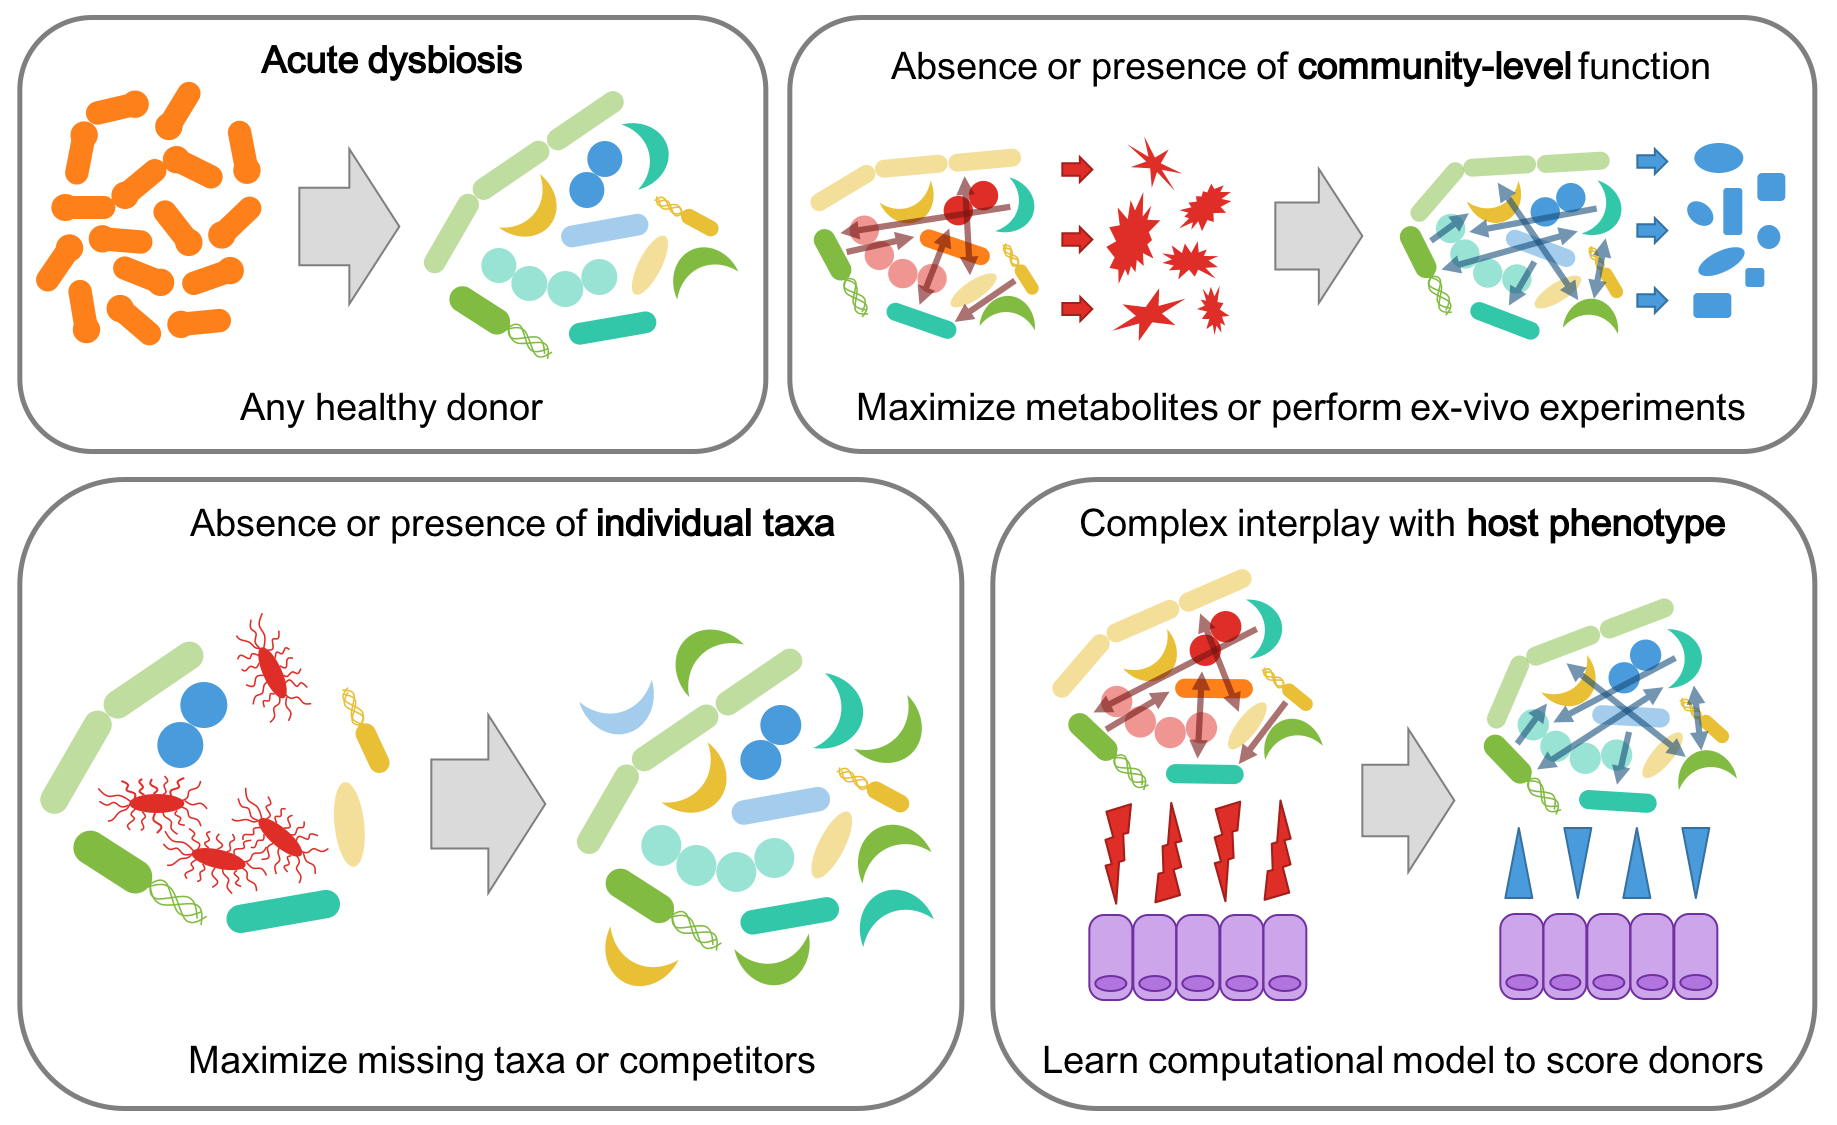
\includegraphics[width=\textwidth]{fig1_overview.png}
    \caption{Overview of the different models of microbiome-mediated disease and associated donor selection strategy.}\label{fig:disease-models}
    \end{center}
\end{figure}

\subsection{Acute dysbiosis}

An acutely dysbiotic gut microbial community is broadly dysfunctional and can no longer maintain the health of the host.
For example, in the case of recurrent Clostridium difficile infection, a disturbed microbial community is unable to prevent colonization by the pathogen, leading to recurrent overgrowth of C. diff and clinical symptoms \cite{Britton2014}.
Acute dysbiosis has also been described with the ``Anna Karenina principle'': all healthy microbiomes are alike but dysbiotic communities are all dysbiotic in their own ways \cite{Zaneveld2017}.
In this view of acute dysbiosis, microbial communities respond stochastically to stressors, resulting in dysbiotic communities which are characterized by increased variability rather than deterministic shifts to precise community type(s) \cite{Zaneveld2017}.

In this model, the host just needs to return to a ``healthy'' microbiome and thus choosing any healthy FMT donor should be sufficient to induce clinical improvements.
Because there is no specific disease-associated microbial community and deviation from health is instead the more important factor, simply replenishing the microbiome with a healthy configuration should be sufficient.
Indeed, FMT trials have demonstrated that recurrent C. diff infection can be effectively treated by almost any choice of donor \cite{Osman2016}.
In this case, researchers should consider how they define a ``healthy'' microbiome and how they will ensure engraftment of the transplanted healthy communities.

\subsection{Absence or presence of individual taxa}

\subsubsection{Absence of beneficial taxa}

In other cases, perhaps a disease is being caused or exacerbated by the lack of certain specific microbes, and replenishing these few taxa would be sufficient to restore the host to health.
For example, Hsiao et al showed that a single microbe, \textit{R. obeum}, restricted infection by \textit{V. cholerae} through quorum-sensing-mediated mechanisms \cite{Hsiao2014}.
Surprisingly, non-communicable diseases may also fall into this model: Wilck et al. demonstrated that a single strain of Lactobacillus was sufficient to prevent salt-induced hypertension, and follow-up studies indicate that similar mechanisms may be involved in salt-sensitive high blood pressure in humans as well \cite{Wilck2017}.

In these cases, the donor selection strategy should focus on maximizing the probability of engraftment of the beneficial taxa.
In cases where the unique taxa are not specifically known or are rare members of the human microbiota, many healthy donors should be pooled together to maximize the probability that the transplanted sample contains the necessary taxa.
If the missing microbes are known and well-characterized, on the other hand, researchers can screen their pool of potential donors to find the sample with the highest abundance of these taxa.

\subsubsection{Presence of harmful taxa}

Rather than being characterized by the absence of individual bacteria, perhaps a disease is instead mediated by the presence or overabundance of specific microbes, and removing these bacteria in a targeted fashion could lead to improvements in disease progression.
For example, \textit{Fusobacterium} has been found to be more abundant in colorectal cancer patients, specifically enriched in the tumors themselves \cite{Kostic2013}.
Multiple groups have identified mechanistic associations between \textit{Fusobacterium}, inflammatory transcriptional signatures, and tumor growth in mouse and human models of colorectal cancer, pointing to a causal role for \textit{Fusobacterium} in colorectal cancer progression \cite{Kostic2013,Rubinstein2013}.
Recent work has found that treating tumors with antibiotics slows tumor progression, further confirming these causal associations and pointing toward potential microbiome-based therapeutic interventions \cite{Bullman2017}.

Removing and replacing these bacteria should be the goal of FMT in cases where this disease model applies.
This can be achieved by first removing the harmful bacteria in a targeted way (e.g. via antibiotic treatment) with follow-up FMT to re-establish a healthy community that prevents their re-colonization.
In all cases, donors should be screened to exclude any samples which contain the harmful bacteria.
Donor samples can then be selected based on the abundance of bacteria which are known to out-compete the harmful taxa.
Competitors can be identified by searching the microbiology literature to identify bacteria which live in the same niche or which have been experimentally shown to directly out-compete the undesirable taxa, or they can perform these competition assays themselves.
If resources to perform competition assays are not available and the literature is sparse, researchers can also mine existing microbiome data to find bacteria which consistently anti-correlate with the harmful taxa, and choose donor samples with a high abundance of these putative competitors.

\subsubsection{Patient matching}

Taxa-based donor selection strategies are particularly amenable to patient-matching, when both patient and donor microbiome data are available prior to the start of a trial.
For example, if one patient is completely missing some of the beneficial taxa but not others, then these taxa can be weighted more heavily in the donor selection process.
The phylogenetic relationships between donor and recipient taxa could also be incorporated into donor selection: if a patient already has many bacteria which are closely phylogenetically related to known competitors of some of the harmful bacteria, then competitors of the other harmful bacteria can be upweighted in the donor selection process.
Similarly, if patients already have taxa which are already filling certain niches important for health, the taxa which fill those same niches can be downweighted in donor selection.

\subsubsection{Case study: Inflammatory Bowel Disease}

An example where the ``missing taxa'' model may be applicable is in inflammatory bowel disease (IBD).
Butyrate has long been associated with inflammatory bowel disease \cite{Scheppach1992}, and recent case-control and longitudinal studies point to a consistent lack of butyrate-producing bacteria in patients with IBD \cite{Duvallet2017,Schirmer2018}.
Furthermore, preliminary FMT trials in IBD have been marked by significant donor variability and suggest that donor microbiome characteristics may be associated with FMT response \cite{Moayyedi2015,Kump2018}.
These results indicate that IBD may benefit from rational donor selection approach, and that donors with high abundances of butyrate-producing organisms may yield higher FMT response rates than randomly selected donors.

Given the availability of microbiome data from completed FMT studies, we tested this hypothesis that IBD trials would benefit from a rational donor selection strategy based on the ``absence of beneficial taxa'' disease model.
We re-analyzed microbiome data from three completed IBD FMT trials which provided publicly available sequencing data for patient and donor samples \cite{Kump2018,Goyal2018,Jacob2017}.
We selected butyrate-producers based on their genus-level taxonomy, using the genera identified in Vital et al. 2017 (see Methods, \cite{Vital2017}).
Donors in the three studies exhibited a range of total abundances of butyrate-producing bacteria (Figure \ref{fig:ibd-butyrate}A).
Surprisingly, however, the abundance of butyrate producers in the donor stool was not associated with recipient patients' clinical responses (Figure \ref{fig:ibd-butyrate}B).
We also found no association with response when matching donor abundances with their respective patient's original abundance of butyrate producers (Supplementary Figure \ref{fig:delta-butyrate}).
These results show that selecting donors based on the abundance of butyrate producers may not yield improved clinical trial outcomes in IBD, and illustrates the process by which clinicians could approach and validate a rational donor selection strategy based on individual taxa.
More complex methods to identify butyrate producers (e.g. using phylogenetic-aware methods and/or metagenomics data) could be used in the next iteration to develop a donor selection strategy, if these data are available to clinicians.
Another approach, discussed below, is to select donors based on functional community assays and direct measurement of butyrate production rather than microbial taxonomies alone.

\begin{figure}
    \begin{center}
    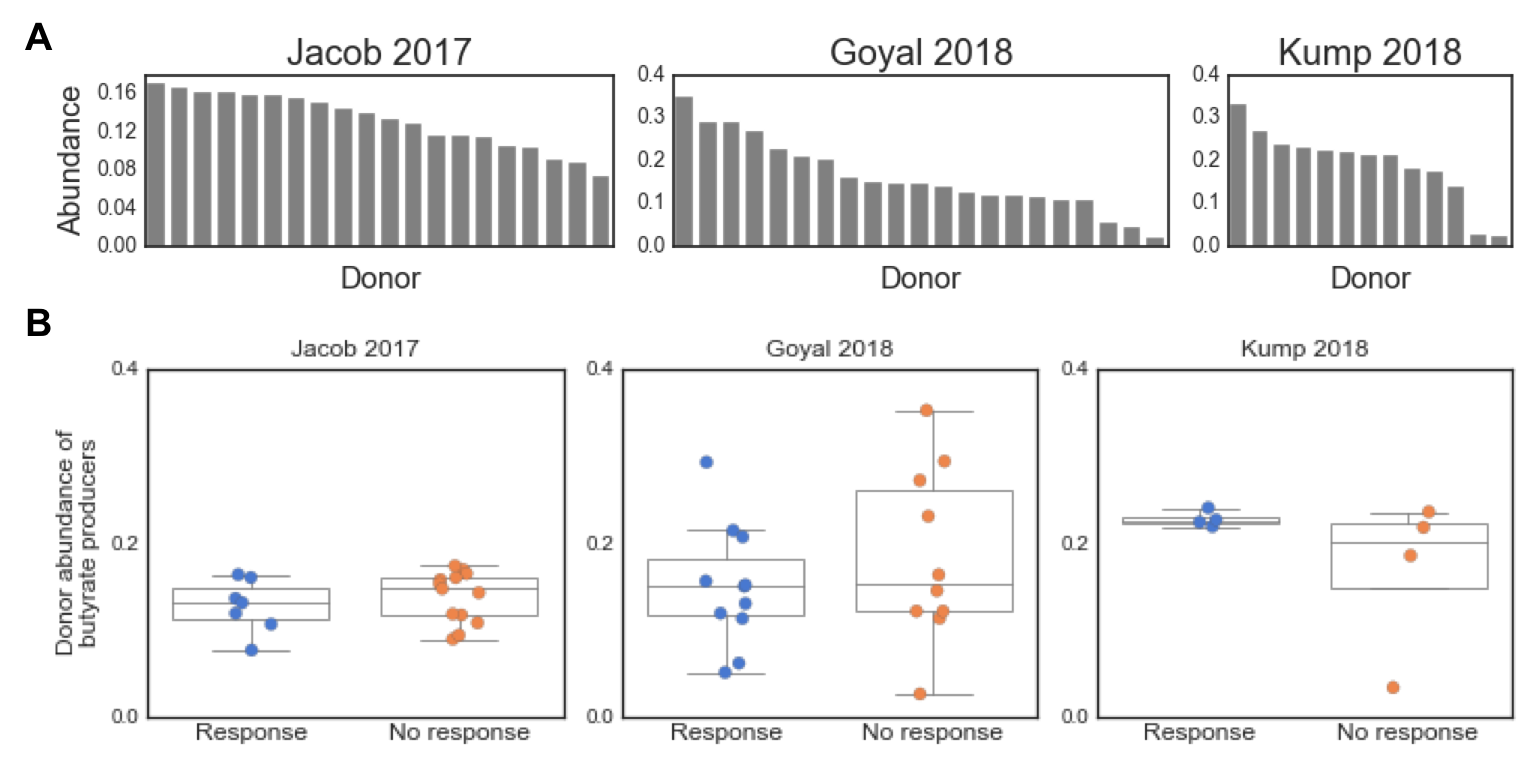
\includegraphics[width=\textwidth]{fig2_ibd_butyrate.png}
    \caption{Case study in IBD: select donors based on abundance of butyrate producers? (A) abundance of butyrate producers in each study's donor samples. (B) abundance of butyrate producers in donor samples, stratified by respective patient's response.}\label{fig:ibd-butyrate}
    \end{center}
\end{figure}

\subsection{Community-level functionality}

Some microbiome-associated diseases may not be addressable by replenishing the patient with a generically healthy community or by targeting individual taxa, and may instead be mediated by the microbiome through a community-level function.
Here, there may not be a consistent disease-associated microbiome across patients in terms of taxonomic composition, but patients may be characterized by having microbiomes which are similarly missing or enriched in some core functionality.
This model may also apply to conditions where there are consistent disease- or health-associated taxa, but in which their collective functioning is the more important mediator of disease.
The IBD case study described above may reflect this situation: although depletion of butyrate producers is strongly associated with IBD throughout the literature, a successful donor selection strategy may need to consider butyrate production directly rather than through the proxy of taxonomy \cite{Duvallet2017,Schirmer2018}.

\subsubsection{Missing community-level function}

In the case where a community-level function is missing from patients' microbiomes, the goal of FMT should be to replace the deficient community with a beneficially functional microbiome.
Here, it is important that a single donor with an intact microbial community is used, rather than a mixture of donors which may not yield the desirable community composition at steady-state after engraftment.
To choose a donor, molecules which can serve as proxies for the metabolic output of the microbial community can be measured directly in donor stool, and donors can be selected based on the abundance of these molecules.

Like IBD, hepatic encephalopathy (HE) is an example where community functionality is likely more relevant to FMT outcome than specific taxa.
A previous trial in HE \cite{Bajaj2017} rationally selected their single donor by maximizing the abundance of \textit{Lachnospiraceae} and \textit{Ruminococcaceae}, taxa which were identified based on cross-sectional microbiome data.
The clinical trial was a success, but it remains unclear from this trial whether the donor's strains engrafted in the patients post-FMT and whether this played any role in the successful FMT responses.
The exact mechanisms of action of these strains remains unknown, though both bacterial families are known short chain fatty acid producers (in particular butyrate) \cite{Vital2017}.
More recent studies have more directly implicated the production of short chain fatty acids and secondary bile acids as being important in liver cirrhosis and subsequent complications such as HE, suggesting that community-level functioning may be a more important driver of FMT response.
Thus, HE may be a case in which function-based donor selection can be employed.

To illustrate this process, we analyzed stool metabolomics data from 83 OpenBiome donors and used this data to rank them based on their estimated production of short chain fatty acids and secondary bile acids (Figure \ref{fig:bn10-liver}).
As in the IBD case study, we found that donors exhibited a range of values for our metabolites of interest (Figure \ref{fig:bn10-liver}A and C).
We ranked donors based on their amounts of the three measured short-chain fatty acids (butyrate, isovalerate, and propionate) and on their bile acid conversion rates, approximated as the ratio between the total amounts of primary and secondary bile acids (Figure \ref{fig:bn10-liver}B and D).
With this process, we were able to identify four donors who were in the top 25\% of all donors for both metrics (Figure \ref{fig:bn10-liver}E).
In a real FMT trial, a clinician would then work with their stool bank to ensure that these donors were still active and/or had enough material to be used in the full trial.

While measuring metabolites in stool as a proxy for community production will likely be an improvement over taxonomy-based approaches in most cases, these measurements are also complicated by potential host effects.
For example, different hosts may absorb these molecules at different rates, and so measuring them in stool may not be an accurate reflection of each donor community's productive potential.
Additionally, community function may depend on non-biologically relevant factors like the donor's diet and time that they provided their sample. As an example, bile acid production spikes after meals \cite{Hofmann1989}, so the amount of bile acids measured in a given stool sample may reflect the amount of time since the donor last ate rather than their actual microbial community's functional production of these molecules.
If clinicians have access to sufficient resources, a better way to screen donors may be to perform ex-vivo assays, in which each donor sample is homogenized and provided with the substrates (e.g. fiber) needed to produce the desirable output (e.g. short-chain fatty acids like butyrate).
In this way, the donor community function can be measured directly \cite{Wang1993,Chen2017}.

\begin{figure}
    \begin{center}
    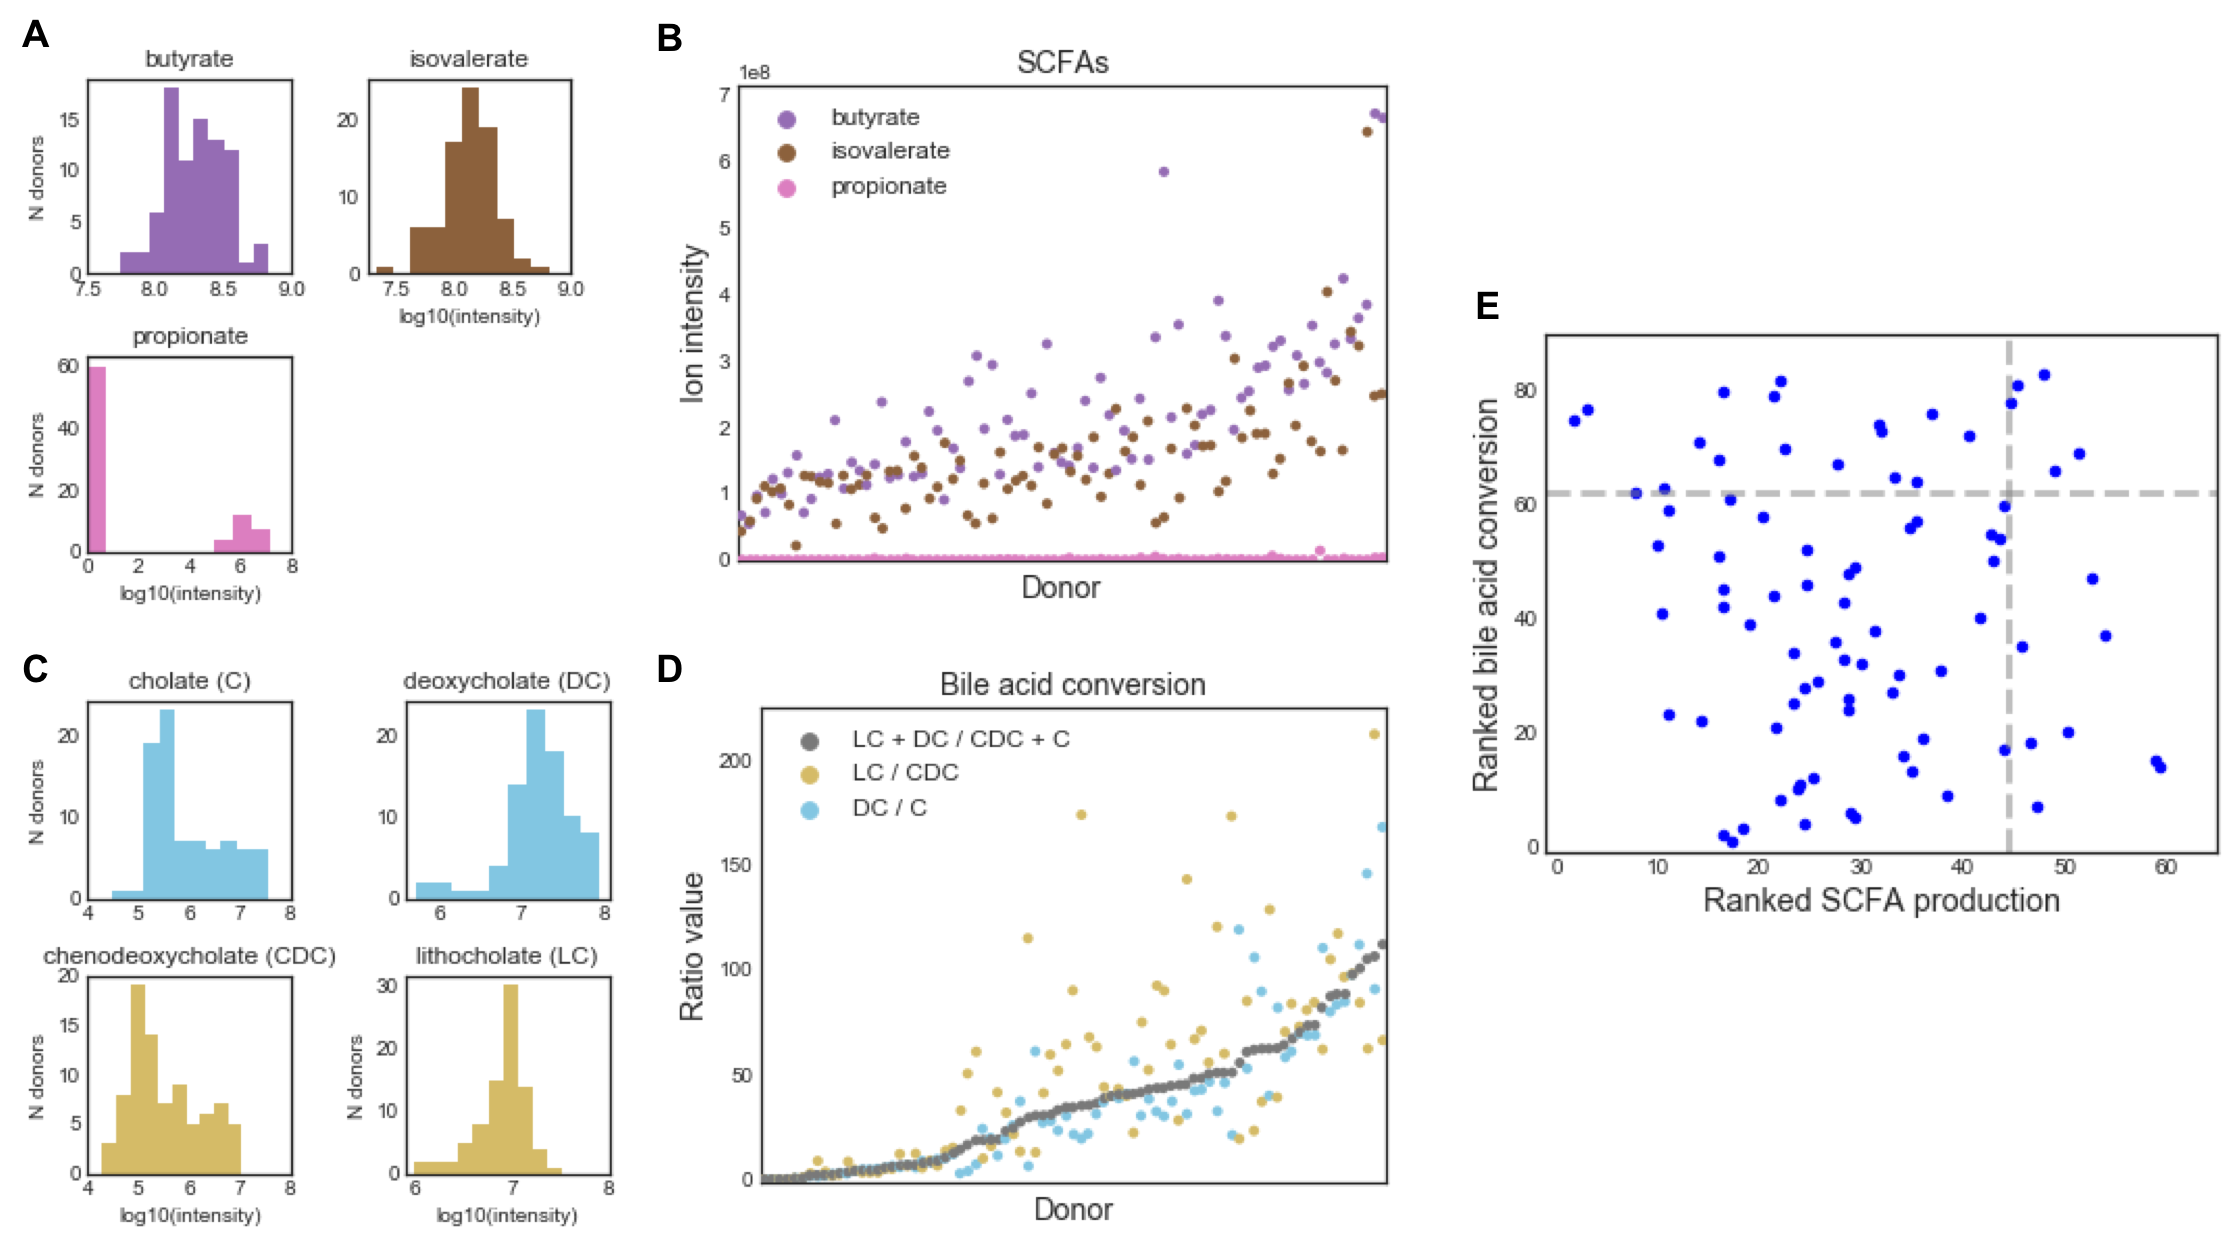
\includegraphics[width=\textwidth]{fig3_cirrhosis_metabolomics.png}
    \caption{Case study in liver cirrhosis: selecting donors based on community function by mining stool metabolomics data. (A) Distribution of SCFAs in all donor stools. (B) Abundance of each SCFA per donor, ranked by average SCFA abundance. (C) Distribution of bile acids in all donors. Primary bile acids are in the left column, secondary bile acids are in the right column. Bile acids are colored according to pathways. (D) Bile acid conversion ratios in each donor, ranked by total secondary to primary bile acids. (E) The five donors in the top 25\% for both of these metrics, for example, could be used in a rationally-designed liver cirrhosis FMT trial.}\label{fig:bn10-liver}
    \end{center}
\end{figure}

\subsubsection{Overactive function}

A disease may also be mediated by an overactive microbiome doing something harmful to the host.
For example, many studies have shown a causal association between TMAO produced by the microbiota and atherosclerosis \cite{Koeth2013,Wang2015}.
Here, the goal of FMT should also be to replace the patient's microbiome with a beneficially functional community, but the donor selection strategy may attempt to identify communities in which the harmful function is completely absent or which produces an inhibitor of the harmful microbe-derived molecule \cite{Wang2015}.

\subsection{Microbiome-associated host phenotypes}

Diseases with more complex etiologies may not have a direct taxonomic or functional association with the microbiome but instead be related through some intermediate host phenotype which needs to be improved or corrected.
For example, severe acute malnutrition has been associated with a gut microbiota which is not fully mature, with mouse experiments suggesting that this association may be causal \cite{Blanton2016,Subramanian2014}.
Other studies have shown a relationship between gut microbiome, immune development, and development of autoimmune conditions later in life \cite{Stokholm2018,Cox2014,Kostic2015}.
These relationships may have mechanistic explanations which are not directly measurable from donor or patient stool (e.g. immunogenicity of bacteria, ability of bacteria to eat the host's mucus, etc) but which can nevertheless be inferred from existing data and used to select potential donors.

For these more complex cases, models can be trained from existing datasets to learn the community signatures linked to the disease-associated phenotype. In some cases, it may be possible to develop computational models which directly predict the phenotype of interest.
For example, Stein et al. developed a model to predict the induction of regulatory T-cells by microbial communities \cite{Stein2018}.
In other cases with few known mechanistic models, machine learning algorithms can be trained on multiple cross-sectional datasets to identify complex signatures that reproducibly distinguish patients from healthy controls.
These models can then be applied to score potential donors, and the donor with the ``most healthy'' score may be chosen for a trial.

\section{Little understanding of underlying disease model}

In some conditions, there may not be enough understanding of the underlying microbiome-based etiology to inform donor selection in an FMT trial. It may also be the case that there are no existing datasets on which to train models, existing datasets are not sufficiently powered to distinguish the different potential underlying models, or logistical considerations constrain a clinician's ability to select specific donors for their trial. In these cases, we recommend selecting different healthy donors, employing an adaptive clinical trial design in which donors are cycled after they have clinical failures (as described previously in \cite{Olesen2017}), and performing retrospective analyses to answer targeted hypotheses which were developed during the clinical trial design process.

\subsection{Cycling healthy donors in adaptive trials}

As donors change through the course of an adaptive trial, clinicians may elect to select their donors randomly or to more rationally cycle through donors \cite{Olesen2017}.
``Differently healthy'' donors may be selected, perhaps representing different underlying disease-associated models described above.
Donors may also be selected to span the range of ``healthy'' microbiomes in a given population.
For example, clinicians may pick a ``median'' health donor (i.e. one who is about as similar to all reference microbiomes), define a ``healthy plane'' and pick donors based on their distance to this plane (as in \cite{Halfvarson2017}), or simply based on the presence or abundance of certain consistently ``core'' health-associated bacteria \cite{Shade2011},\cite{Duvallet2017}.
In a similar vein, ``healthy'' donors can also be chosen based on their distance from disease-associated microbiomes, as opposed or in addition to similarity to health. Published case-control datasets can be used to identify donors with communities which are farthest away from the median or average diseased patient.
These datasets can also be mined to identify taxa which are consistently disease-associated, and which should be minimized or perhaps even absent in the potential donor.
Pairing rational donor selection with adaptive trial designs may eventually yield insight into the underlying model mediating the disease of interest if certain types of ``healthy'' donors consistently perform better at treating patients than others.

\subsection{Discovery-based retrospective analyses}

In these exploratory FMT clinical trials, discovering microbiome characteristics which are differentially associated with FMT response may be a valuable secondary endpoint \cite{Olesen2018}, identifying characteristics of good donors and informing donor selection strategy for future trials.
Furthermore, companies attempting to develop microbiome-based therapeutics may use FMT trials to discover the key bacteria which mediate FMT response in order to include these in their microbial cocktail product.
However, exploratory FMT trials tend to enroll few patients, limiting the potential power of retrospective analyses to find associations between the microbiome and FMT response.

We performed a simulation to determine the likelihood of a retrospective analysis to identify donor-derived bacteria associated with different patient responses to FMT.
We performed this simulation for multiple FMT trial set-ups and outcomes (i.e. number of FMT responders and non-responders).
We used existing microbiome datasets to model different effect sizes, where we use ``effect size'' to mean the number of bacteria which are differentially abundant in donor samples given to patients who did and did not respond to FMT.
We used case-control datasets to model the microbiome data and various effect sizes, with a large effect represented by an infectious diarrhea dataset \cite{Schubert2014}, a medium effect represented by colorectal cancer \cite{Baxter2016}, and a weak effect represented by obesity \cite{Goodrich2014}.
For each of these datasets, we identified the top ten most differentially abundant bacteria in the overall population as the key mediating bacteria (see Methods).
Next, we simulated different trials, varying the numbers of patients in the FMT arm and the FMT response rates (i.e. proportion of patients which were FMT responders, represented by sampling from the ``case'' patients, vs. non-responders, represented by sampling from the ``control'' patients, representing non-responders).
We subsampled patients according to these parameter settings, identified differentially abundant genera, and compared these to the top ten genera identified from the entire datasets (Figure \ref{fig:power-sim}).

In cases where the microbial signature for FMT response is expected to be large (i.e. the difference in donor stools given to FMT responders vs. non-responders is as large as the effect of diarrhea effect on the microbiome), we found that small FMT trials would recover most of the top hits in most cases.
The power to detect associations decreased as FMT response rates became less balanced (i.e. response rates different from 50\%), and in these cases trials would need to include up to 50 patients in the FMT arm to recover the key mediating taxa.
For both medium and small effect sizes, however, prohibitively large FMT arms would be needed to recover most key mediating taxa.
We found that when the microbial signature for FMT is equivalent to the effect of diseases like colorectal cancer on the microbiome, at least 100 patients are needed in the FMT arm to recover at least half of the most truly differentially abundant genera for most FMT trials.

These results suggest that successful secondary analyses of microbiome data from FMT trials will require either very large FMT arms, investigating more targeted hypotheses, or additional sample collections.
For example, clinicians may consider pairing donor and patient samples or collecting longitudinal patient samples to increase power to make discoveries.
They may also consider testing specific hypotheses developed before the trial, such as comparing the total abundance of butyrate producers between FMT responders and non-responders, or performing functional assays to measure specific metabolites thought to be associated with FMT response.
On the other hand, researchers wishing to identify the key taxa to include in an FMT drug may consider pursuing clinical trials in which identifying these taxa is the primary endpoint, and power them accordingly.


\begin{figure}
    \begin{center}
    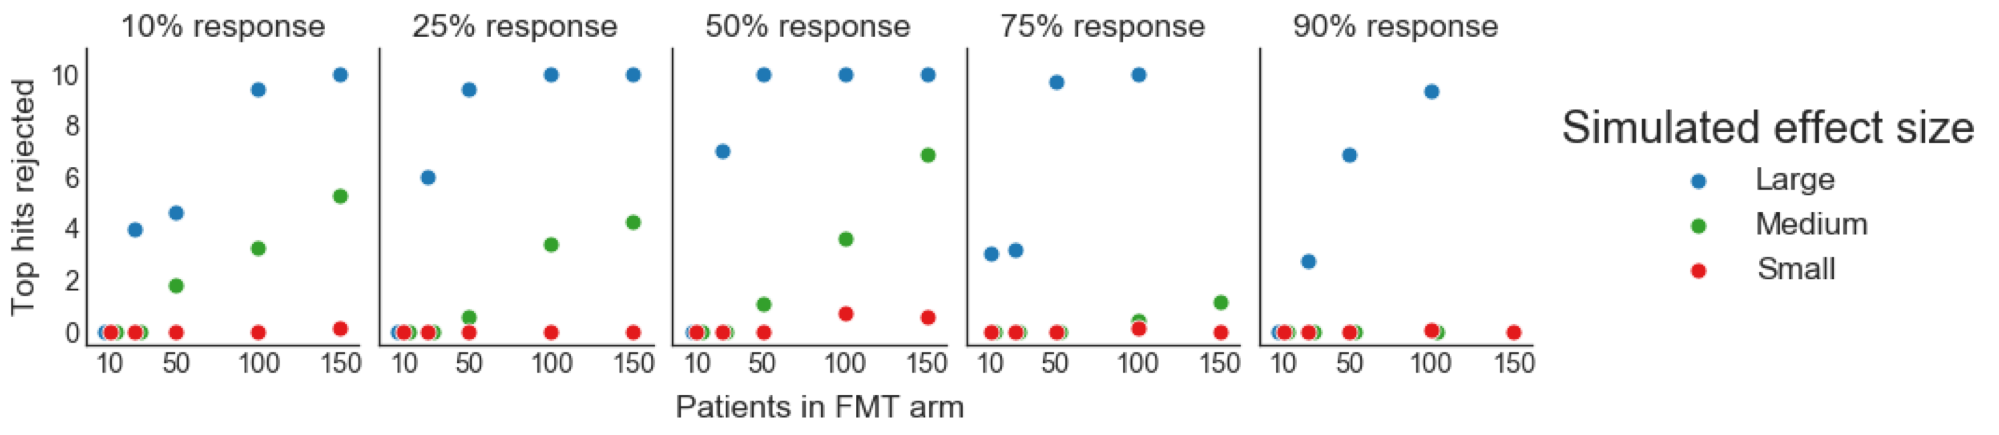
\includegraphics[width=\textwidth]{fig4_power_simulation.png}
    \caption{Power simulation results, showing how many of the 10 most ``truly'' differentially abundant genera would be recovered as significant under different FMT study designs. Each panel represents a different FMT response rate (i.e. percent of patients in the responder vs. non-responder group). The effect size (i.e. number of genera which are differentially abundant in FMT responders vs. non-responders) was simulated by using three different case-control microbiome datasets. A large effect size is modeled by the effect of diarrhea on the microbiome, medium by colorectal cancer, and small by obesity. The top 10 "true" differentially abundant genera were identified by calculating their signal-to-noise ratios in the full original dataset (i.e. mean difference divided by the standard deviation).}\label{fig:power-sim}
    \end{center}
\end{figure}

\section{Discussion}

The framework presented here encourages clinicians to leverage their clinical experience, existing microbiome research and published datasets, and the increasing availability of screened donor stools to more efficiently translate microbiome-based interventions into clinical impact.
Clinicians can apply their existing knowledge and a priori hypotheses to determine which microbiome-mediated disease model may underlie their indication of interest, and then select donors accordingly.
By rationally choosing donors during the FMT trial design, clinicians will increase the likelihood of successful FMT trials in diseases in which donor heterogeneity affects patient response.
Our power simulation analysis also suggests that specific plans for retrospective analyses of the microbiome data generated should be developed during trial design, with targeted hypotheses of interest and sample collection plans tailored accordingly.
Otherwise, exploratory analyses are unlikely to make new discoveries from most FMT trials. Paired with adaptive clinical trial designs, FMT trials with rationally-selected donors will become an important tool in advancing translational microbiome research and clinical treatment to improve and save patient lives.

As clinical trial design methodologies for FMT trials become more developed, many additional questions will need to be addressed.
Many of these key questions relate to the nuances involved in choosing healthy donors: what defines a ``healthy'' donor, and what should define one?
These questions are critical because regardless of the underlying model, in all cases a healthy donor must be identified.
However, as our understanding of the microbiome in societies around the world continues to increase, consensus on the exact structure of a ``healthy'' microbiome decreases.
Should donors be selected to reflect the patient populations, or simply be devoid of pathogens and source from as ``healthy'' of donors as possible?
We know that Europeans and North Americans tend to have less \textit{Prevotella} than healthy Africans from across the continent in both urban and rural communities \cite{Yatsunenko2012,Ou2013,DeFilippo2010}.
Thus, should a clinician carrying out an FMT trial in an African setting use local African cohort as their donor population in order to better match the expected ``healthy'' state of their participants?
In some cases, using a local population may be incompatible with established donor screening criteria because of geographical differences in baseline microbial community composition, prior likelihood of pathogen colonization, or differences in diet and lifestyle habits leading to different dominating strains.
Should clinicians consider relaxing donor screening and exclusion criteria in cases where donors are sourced from countries where commensal colonization by potential pathogens is common population-wide?
More research to understand the functional differences and clinical implications of different ``healthy'' communities across global populations and specifically in the context of FMT trials will be required before these and many related questions can be answered \cite{Bello2018,Rabesandratana2018}.

On the patient side, comorbidities, lifestyle, and dynamic disease manifestations may present challenges and opportunities to improve donor selection processes.
How should comorbidities be incorporated into donor selection?
Patients with multiple disease processes may be dominated by one microbiome-mediated disease model or may exhibit a combination of models, perhaps affecting which donors would be optimal for their specific case.
For example, a person with one community-level function process and one acute dysbiosis process may respond well to total community replacement alone, or may require a combination of total community replacement along with enrichment for community function.
Additionally, will diseases that change manifestations over time benefit from employing different donor selection strategies over the course of a longitudinal FMT trial?
Although there have been no serious adverse events related to FMT material in either clinical practice for rCDI or in clinical trials across adults or pediatrics, could some donors further reduce the probability of adverse events in at-risk patients?
Finally, how should other sources of heterogeneity like lifestyle, diet, and medication usage be incorporated into rational donor selection?
In cases where FMT is combined with other microbiome-targeted interventions like prebiotics or dietary changes, could some donors have synergistic effects with these paired interventions and lead to greater clinical success?

To ensure that FMT reaches its full potential to improve and save patient lives, clinicians should think critically about how their FMT trials can be designed for maximal impact.
By applying new approaches like rational donor selection and adaptive trial designs, the number of trials which fail even though they could have succeeded will drastically decrease.
Furthermore, by developing targeted hypotheses, post-trial analysis plans, and associated sample collection schema alongside the core FMT trial design itself, the number of basic scientific discoveries that are made from each trial will significantly increase.
As FMT expands far beyond rCDI and microbiome-based therapeutics are developed to target a range of disease, novel methods and approaches tailored to the unique challenges and opportunities presented by FMT will be critical to ensuring the advancement of translational microbiome science and beneficial impact on patient lives.

\section{Methods}

\subsection{Microbiome data processing}

Raw fastq data files were downloaded from the European Nucleotide Archive using the following accession numbers: Jacob et al 2017, PRJNA388210; Goyal et al. 2018, PRJNA380944; and Kump et al. 2018, PRJEB11841.
All data was processed using QIIME 2 (v. 2018.6.0, \cite{qiime2}).
Briefly, data was imported into QIIME 2 as paired-end (Kump et al. 2018; Jacob et al. 2017) or single-end (Goyal et al. 2018) data, filtered based on sequence quality with \texttt{quality-filter q-score}, and denoised with deblur using \texttt{deblur denoise-16S} \cite{deblur}.
Representative sequences were assigned taxonomy using \texttt{feature-classifier classify-sklearn} with the GreenGenes-trained Naive Bayes classifier provided by QIIME 2 (gg-13-8-99-nb-classifier.qza) \cite{feature-classifier}.
All data was exported to tab-delimited format and analyzed in Python 2.7.6.

\subsection{Quantifying abundance of butyrate producers}

We identified butyrate producers at the genus-level based on the analysis performed in Vital et al. 2017 \cite{Vital2017}.
These taxa were detected in >70\% of individuals in Vital et al. 2017, are known butyrate producers (with a majority of the analyzed representative genomes containing known butyrate production pathways), and accounted for the majority of the total butyrate pathway abundances in human metagenomics data.
We removed \textit{E. ventriosum}, \textit{E. hallii}, and \textit{E. rectale} from our analyses as these species-level taxa do not comprise one genus with conserved butyrate production.

\subsection{Stool metabolomics}

Metabolomics data was generated as described in Poyet, Groussin, Gibbons et al. (in preparation) and downloaded after personal communication with the authors.
For donors with multiple samples, we considered the mean metabolite abundances across all sampled time points.
We identified three short chain fatty acids in the data (propionate, butyrate, and isovalerate) and the major primary (cholate and chenodeoxycholate) and secondary (deoxycholate and lithocholate) bile acids.
Lithocholate was available for both C-18 negative and HILIC negative modes; we considered only the C-18 negative data to match the other bile acids.
Bile acid conversion rates were calculated as in Kakiyama et al. 2013 \cite{Kakiyama2013}.
Donors were ranked based on their average SCFA abundances and based on the total bile acid conversion ratio ( (lithocholate + deoxycholate) / (chenodeoxycholate + cholate) ).

\subsection{Power simulation}

We performed a simulation to determine the power of FMT trials to retrospectively find associations between donor bacterial abundances and FMT response.
We used case-control gut microbiome datasets from MicrobiomeHD \cite{Duvallet2017} to model different effect sizes for FMT response.
Here, we use ``effect size'' to mean the number of genera which are differentially abundant between patients who respond to FMT vs. patients who do not.
Per the results in MicrobiomeHD, we used infectious diarrhea to model a large effect \cite{Schubert2014}, colorectal cancer to model a medium effect \cite{Baxter2016}, and obesity to model a small effect \cite{Goodrich2014}.
We collapsed OTUs to genus-level as in \cite{Duvallet2017} and ranked genera according to their signal-to-noise ratio in each entire dataset, where the signal-to-noise was calculated as the difference in mean log abundance in cases and controls divided by the standard deviation of the log abundances across all samples.
We considered the 10 genera with the largest absolute signal-to-noise ratios as our ``top hits'' in the main text.

We modeled different FMT clinical trial designs and outcomes by varying the number of total patients in the trial and the percent of FMT responders (i.e. the number of patients we selected from the original ``case'' group relative to the original ``control'' patients, to model FMT responders and non-responders).
For each of these designs, we subsampled the correct number of case samples to represent FMT responders and control samples to represent non-responders from the original datasets.
We identified significantly differentially abundant genera with the \texttt{kruskalwallis} function from \texttt{scipy.stats.mstats} (scipy v. 1.1.0) as genera with q $<$ 0.05 after multiple hypothesis testing correction with the \texttt{multipletests} function (\texttt{method=`fdr\_bh'}) from the \texttt{statsmodels.sandbox.stats.multicomp} package (statsmodels v. 0.9.0).
We then counted how many of the top genera identified through the signal-to-noise ranking were identified as significantly different as a proxy for the power to detect effects.

\subsection{Code and data availability}

Code to reproduce all of these analyses and figures can be found at \url{https://github.com/cduvallet/donor-selection/}.
Data were downloaded from original sources as described above.

\newpage
\section{Supplementary Figure}

\FloatBarrier
\begin{figure}[h]
    \begin{center}
    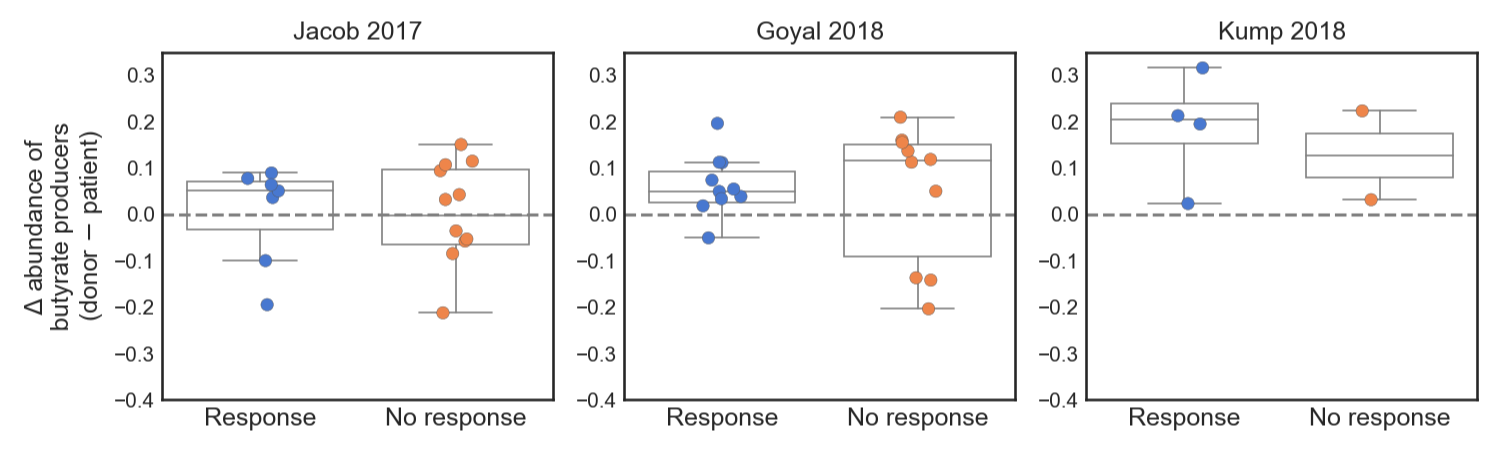
\includegraphics[width=\textwidth]{suppfig_delta_butyrate_vs_response.png}
    \caption{Difference between abundance of butyrate producers in donor sample and respective patient sample, stratified by patient response.}\label{fig:delta-butyrate}
    \end{center}
\end{figure}

\begin{singlespace}
\bibliographystyle{unsrtnat}
\bibliography{donor-selection/donor-selection-refs.bib}
\end{singlespace}


%% This is an example first chapter.  You should put chapter/appendix that you
%% write into a separate file, and add a line \include{yourfilename} to
%% main.tex, where `yourfilename.tex' is the name of the chapter/appendix file.
%% You can process specific files by typing their names in at the
%% \files=
%% prompt when you run the file main.tex through LaTeX.

\graphicspath{{24hr/figures/}}

\chapter{Residential sewage provides a view into community-level human microbiome and metabolome}\label{chap:24hr}

\noindent
Mariana G Matus, Claire Duvallet, Melissa Soule, Noriko Endo, Newsha Ghaeli,  Ilana Brito, Carlo Ratti, Elizabeth B Kujawinski, Eric J Alm

\bigskip
\bigskip
\noindent
The contents of this chapter constitute a manuscript in preparation for submission.

\clearpage

\section*{Abstract}

Wastewater-based epidemiology has long been proposed as a tool for population health monitoring, with applications ranging from infectious disease surveillance to drug consumption estimation. To date, however, there are few examples of wastewater epidemiology being implemented in practice. Here, we propose a novel platform that adapts existing wastewater-based epidemiology approaches for community-level public health surveillance. We integrate sewage network and population information to identify a sampling manhole representative of a residential community and show that the wastewater sampled at this upstream manhole contains more human-derived bacteria and metabolites than downstream wastewater treatment plant samples, which are the usual sampling locations in wastewater epidemiology. Our method to perform untargeted metabolomics on raw sewage allows for the identification of multiple glucuronide compounds, which are indicative of direct human excretion and typically too unstable to be detected in wastewater. We show that these compounds are absent in downstream samples, but abundant in our residential sewage samples. Next, we perform an hourly 24-hour sampling campaign to identify human and environmental components of the sewage metabolome and microbiome based on diurnal variations. We confirm urinary and fecal metabolites and find that their dynamics reflect human behavior but differ from each other. Finally, we propose that mining untargeted data derived from residential sewage opens additional possibilities for identifying biomarkers with direct public health or policy relevance and show preliminary results from the metabolomics data. Together, these results suggest a novel approach for implementing wastewater epidemiology in urban settings that provides a new source of community-level health data and which could be developed into a citywide public health observatory.

\section{Introduction}

Urbanization is a globally increasing phenomenon. By 2050, 70\% of the world's population will live in cities where 80\% of the global GDP will be generated. Cities are thus prime locations to deliver services that improve the wellbeing of residents. However, public health officials in cities tend to operate under financial constraints and with limited data to establish priorities and measure the impact of their programs. Wastewater has been proposed as a source of data on population health and behavior that can fill this gap at relatively low cost for public health officials \cite{Daughton2018}.

Wastewater-based epidemiology could have enormous benefit to public health practice, providing real-time assessment of population health and generating data to support public health and city policies. Currently, most public health surveillance is based on reports from hospitals and other clinical centers, and appropriate responses are initiated after enough clinical cases have been reported. Wastewater-based public health surveillance platforms, in contrast, could provide real-time data on emerging outbreaks before a critical mass of patients have gotten sick \cite{Manor2014,Hellmer2014}. Viral and bacterial pathogens shed in stool could be directly detected in sewage, triggering the deployment of coordinated awareness campaigns or other public health interventions to areas with the largest number of sick patients, all without needing to wait for case reports from hospitals. In addition to identifying emerging outbreaks, wastewater could provide a novel source of data to evaluate the effectiveness of policies intended to have long-term effects on a population's health \cite{Daughton2018}. For example, rather than waiting years to measure the impact of taxing sugary drinks on population obesity levels, biomarkers of obesity or consumption could be directly measured in sewage before and after the policy roll-out, thus providing a more immediate measure of the impact of policy on targeted outcomes.

Wastewater-based epidemiology has been proposed for many exciting applications. It has been shown to be useful as an early indicator of poliovirus outbreaks to target vaccination campaigns in polio-free countries \cite{Manor2014,Kaliner2015} and to quantify asymptomatic circulation \cite{Berchenko2017}. Environmental surveillance of typhoid and antimicrobial resistance through urban wastewater are emerging areas of interest in global and public health organizations \cite{Pehrsson2016,Initiatives2018}. Besides infectious disease, methods have been developed and standardized over the last decade to successfully provide continuous data on illicit drug consumption at the national- and regional-level in Australia \cite{AustralianReport} and over 60 European cities and towns \cite{vanNuijs2018,Thomas2012,BazLomba2016}. The academic community is now interested in branching out to measure lifestyle chemicals and biomarkers of health such as obesity levels \cite{Daughton2018,Arnaud2018,Newton2015}. More recently, wastewater testing has been proposed as a promising tool to tackle the opioid epidemic that is severely affecting the U.S \cite{Keshaviah2016,Keshaviah2017}. However, apart from successful poliovirus surveillance and, to a lesser extent, national-level drug consumption surveillance programs, most application areas remain proof-of-concept academic projects and have yet to be implemented into public health and other public service delivery agencies.

Despite great technical advances over the past decades, wastewater testing still presents considerable challenges that decrease its usefulness to public health officials and policy-makers. In most proposed applications, wastewater is sampled at downstream sites like pump stations or treatment plants \cite{Manor2014,Hellmer2014}. While downstream collection sites are easily accessible and cost-effective, they impose barriers to data interpretation in the public health context. Wastewater at treatment plants is a combination of residential households and commercial and industrial buildings, and it may represent one or more municipalities. These factors create technical biases in the data and prevent clear consumption or infection rates from being calculated from measured quantities. Additionally, if the interest is to compare several cities, collection from different wastewater treatment plants or other downstream sites may introduce confounding factors, such as representation of different population sizes \cite{OBrien2013}, large variation in wastewater travel time from different sources, different rates of in-sewer degradation of chemical \cite{Thai2014} and bacterial biomarkers, and collection with ad-hoc sampling equipment that prevents researchers from optimizing collection parameters to obtain representative samples \cite{Ort2010}. Finally, while collecting composite samples from wastewater treatment plants (WWTPs) is practical and cost-effective to generate national estimates \cite{Zuccato2008,Castiglioni2006,Thomas2012}, data from WWTPs is not optimal for city officials since it lacks geographic specificity. Finally, public health officials are interested in a broad range of human health biomarkers but it is not straightforward to know what markers are stable and quantifiable in wastewater collected from different regions \cite{Arnaud2018}.

Here, we propose a novel implementation of wastewater epidemiology that addresses these challenges and develops wastewater testing as a platform to directly measure the health of urban communities and facilitate applications to public health. We combine demographic, sewage, and geographic data sources to curate and select an upstream sampling site that reflects a residential population. By mining untargeted microbiome and metabolomics data, we show that residential sewage reflects human diurnal activity and identify human-derived biomarkers which can be specifically separated from environmental contributors. Together, this work is the first to show that upstream wastewater sampling could provide a novel useful data source for public health agencies.

\section{Results}

\subsection{Upstream residential catchments provide more useful public health information than WWTP samples}

Integrating GIS datasets with demographic and sewage network information enables the selection of sampling sites with carefully curated technical and population characteristics. We defined residential catchments as those which represent areas with at least 80\% residential land use, a population of over 5,000 people, and a maximum sewage travel time of less than 60 minutes (Fig. \ref{24hr:fig1}A). We screened all manholes in our municipality and selected a manhole which met these criteria (Fig. \ref{24hr:fig1}A). From a usability perspective, data from residential catchments will be more actionable by municipal public health departments because sites can be selected to mostly capture resident rather than transient populations, and to have the spatial resolution that matches their public health interventions.

Besides providing geographical specificity to the sample, residential catchments mitigate variability in population size and sewage travel time observed at WWTPs. Our selection criteria produces catchments with similar population sizes by design (5,000--10,000 inhabitants) rather than the large range observed (1,000--2,000,000 inhabitants) in WWTPs (Supp. Fig. \ref{24hr:figS1}, \cite{Newton2015}). Additionally, residential catchments are more likely to contain even representation of all households in the catchment compared to WWTPs: in our residential catchment, sewage from every source travels at most 45 minutes to the sampling point and the distribution of travel times is narrowly-distributed (Fig. \ref{24hr:fig1}A). Sewage at WWTPs, on the other hand, can have travelled anywhere from minutes to hours before it reaches the sampling point. Sampling in residential catchments therefore mitigates the need to correct for unequal population sizes and travel times to some extent.

Residential sewage contains more direct chemical markers of human consumption and behavior than sewage sampled at WWTPs. We sampled a residential sewer (selected as described above) and a downstream pump station (Fig. \ref{24hr:fig1}B) and performed untargeted metabolomics and 16S rRNA sequencing on the filtrate and bacterial cells, respectively. 34.5\% of the metabolites detected in both sewer and WWTP samples (n=245/710) had significantly different concentrations (p-value $<$ 0.05 independent T-test with FDR correction for multiple testing). Of these differentially abundant metabolites, 73\% (n=179/245) decreased or disappeared completely from wastewater collected at the WWTP, including many metabolites from human activity as defined later in this paper (Fig. \ref{24hr:fig2}A yellow dots, Fig. \ref{24hr:fig3}B yellow bars, Supp. Fig. \ref{24hr:figS2} cluster M1). Similarly, we found that residential sewage contained a higher proportion of human-associated bacteria than WWTP sewage. On average, 66\% of the microbial community from residential sewage was of human fecal origin, compared to 51\% in the pump station samples (Fig. \ref{24hr:fig2}B), with the Ruminococcaceae, Lachnospiraceae, Prevotellaceae, Veillonellaceae and Erysipelotrichaceae families being reduced (Supp. Fig. \ref{24hr:figS3}). These results are similar to those reported in Newton et al. \cite{Newton2015}, where on average 15\% of sequences in WWTP sewage had human fecal origin. Together, these results indicate that wastewater from residential catchments which has been traveling in sewers for less than one hour contains many human biomarkers that are absent in wastewater collected at WWTPs.

Furthermore, performing untargeted metabolomics on residential catchment samples extends the possible biomarkers that can be monitored through wastewater epidemiology. We identified 22 glucuronide compounds in our untargeted data (see Methods). Glucuronides are chemical groups added to exogenous molecules by the human liver to aid in their excretion and are thus indicators of human excretion, distinguishing between molecules simply discarded into the sewers versus those consumed and excreted by humans and providing direct evidence of consumption. However, many bacteria carry glucuronidase enzymes that release the glucuronide group to use as carbon source \cite{Pollet2017}, and these unstable molecules have previously been difficult to identify in sewage samples from WWTPs \cite{Jacox2017}. In our data, the majority of the identified glucuronides were significantly reduced or altogether absent in wastewater collected at the WWTP (Figure \ref{24hr:fig2}C). Sampling upstream allows for the detection of these unstable molecules and also more generally expands the number of compounds which can be measured. Molecules which are usually difficult to measure by mass spectrometry in wastewater because they do not ionize well should be captured in residential catchments, since the human body excretes compounds by dissolving them in urine or stool and therefore naturally converts exogenous compounds into more ionizable chemical forms. Thus, detecting a large number of glucuronides in our residential catchment sewage sample suggests that expanding wastewater monitoring to chemical variants of molecules of interest may be beneficial for future environmental surveillance applications.

\subsection{Residential sewage microbiome and metabolome contain both human- and environmentally-derived components}

Chemical and bacterial biomarkers detected in residential sewage reflect the daily timescale of human activity. We used the average sewage flow rate over two months as a proxy for human activity (Figure \ref{24hr:fig3}). We hypothesized that human-associated metabolites and bacteria would increase during the day, when the contributing population would be more active, and decrease at night. We collected hourly samples over 24 hours from the residential catchment manhole and produced 16S rDNA sequencing and untargeted metabolomics profiles (Figure \ref{24hr:fig3}A). We co-clustered metabolomic features (n=3,672) and microbial OTUs (n=254) based on their Spearman correlation (Fig. \ref{24hr:fig3}B \& D, Supp. Fig. \ref{24hr:figS2}), and found that the metabolic features grouped into two main clusters (M1 and M2), while bacterial OTUs produced three groups (O1 and O2 are highlighted). The M1 metabolite cluster (n=2,815) had strong positive correlation with the O1 bacterial cluster (n=41) and negative correlation to the O2 bacterial cluster (n=84). The majority of metabolites and bacteria in these groups also correlated with the average flow rate in the sewer, increasing during the day and becoming drastically less abundant at night (Fig. \ref{24hr:fig3}B \& D).

Metabolites and bacteria in sewage separate into human and environmental contributions. Groups M1 and O1 were enriched in human-derived bacteria and metabolites, while groups M2 and O2 contained bacteria and metabolites derived from the environment (Fig. \ref{24hr:fig3}C). The cluster M1 was statistically enriched in matches to human metabolites compared to the M2 cluster (Fig. \ref{24hr:fig3}C), and includes known urinary and fecal metabolites. Twenty-two metabolic features in M1 were identified as glucuronide compounds of hormones, bile acids and pharmaceuticals, which are direct markers of human excretion as discussed above. Bacteria in the cluster O1 were putatively identified as coming from human gut microbiomes. Cluster O1 included 41 bacterial OTUs primarily from the Firmicutes and Bacteroidetes phyla, which are major components of the human gut flora (Fig. \ref{24hr:fig3}D). Additionally, the top 10 most abundant bacterial families in human stool (Human Microbiome Project) made up 65\% of the community in the O1 group (Supp. Fig. \ref{24hr:figS4}). Similar to what was observed in the metabolites, O1 bacteria had a dip in relative abundance during nighttime (Figure \ref{24hr:fig3}B). Clusters M2 and O2, on the other hand, remained relatively constant through the day and likely reflect bacteria and metabolites sourced from environmental background rather than human activity. Cluster M2 had few putative human-associated hits, and had constant abundance through the day and nighttime. The molecules in this group likely represent chemicals derived from the environment or sewer biochemistry. Human-associated bacteria were similarly decreased in cluster O2: most of the OTUs were Proteobacteria, which are not major members of the normal gut flora, and human fecal bacterial families comprised only 1.4\% of the abundance of this cluster (Supp. Fig. \ref{24hr:figS4}). The relative abundance of cluster O2 increased at night, reflecting that these environmental made up a larger proportion of the residential sewage microbiome during periods of low human activity (Fig. \ref{24hr:fig3}D).

\subsection{Identification of potential public health biomarkers in residential sewage}

Urine and fecal contributions to residential sewage can be identified through untargeted analyses. We identified and confirmed metabolites corresponding to human urinary and fecal markers through a combination of MS2 matching and confirming with analytical standards. In our attempts to annotate metabolite features, we prioritized features with high abundance across all samples and in a few samples of interest (i.e. 8 am and 2 pm samples, which contained more metabolites and which we expected to correlate with human behavior). We screened the top mz values against METLIN and HMDB databases to find putative human-derived metabolites \cite{Wishart2012,Smith2005}. We confirmed features which putatively matched urinary or fecal markers and for which we could acquire analytical standards. Furthermore, we compared the MS2 fragmentation patterns for potential glucuronide compounds with their expected fragmentations and used diagnostic mz peaks to putatively confirm these compounds (see Methods). The most abundant feature in our dataset was confirmed via analytical standard as alpha-N-phenylacetyl-L-glutamine (PAG), a metabolite of phenylacetic acid and an end product of phenylalanine metabolism excreted in urine \cite{Seakins1971,Stein1954}. Previous studies on human physiology have found that PAG excretion remains constant in response to diet and does not exhibit diurnal cycling in individual patients \cite{Seakins1971}. Thus, the abundance of PAG in our sample likely correlates with the total volume of urine in sewage at any given time. Urobilinogen, a breakdown product of hemoglobin excreted primarily in stool \cite{Balikov1957}, was also confirmed via analytical standard. We also confirmed 4 bile acids (chenodeoxycholic acid, cholic acid, glycocholic acid, taurocholic acid), which represent the major primary conjugated and unconjugated bile acids produced by the liver to aid in digestion and which we considered as putative fecal markers.

The urinary and fecal metabolites reflected general diurnal human dynamics, but differed from each other (Figure \ref{24hr:fig4}). Both types of metabolites decreased at night, with the fecal markers almost completely disappearing while the urinary marker remained detectable. Fecal markers also showed significant spikes in the 8 am and 3 pm samples, and were slightly elevated throughout the evening (8 - 10 pm). The urinary marker, on the other hand, increased in the morning and stayed relatively consistent throughout the day. These patterns correspond with known patterns of human behavior: at night, people are less likely to wake up to defecate but do wake up to urinate. During the day, urination remains relatively constant across the entire population, but defecation probably spikes in the morning right after waking up and after meal times.

Furthermore, the daily dynamics of bile acids in residential sewage may reflect population-level behavior and physiology. During the day, levels of unconjugated cholic and chenodeoxycholic acids remained relatively constant but conjugated cholic acids (glycocholic and taurocholic acid) spiked after mealtimes (Fig. \ref{24hr:fig4}). In individuals, the liver synthesizes more bile acids from cholesterol after it is ingested during a meal \cite{Hofmann1989}. Levels of taurocholic acid are also known to increase significantly after meals, since the diet is the primary source of taurine in humans. The liver secretes only the conjugated forms of cholic acid, glycocholic and taurocholic acid, into the gut. Thus, the post-meal spikes in conjugated bile acids in our data may reflect not only more stool in the sewage but also an aggregate population-level increase in physiological production of bile acids by the liver in response to meals. The daily dynamics of fecal bile acid excretion has not been studied in humans, in part because it is difficult to access finely temporally-resolved data given that humans defecate only 1-3 times per day on average. These data suggest that analyzing physically aggregated biological data could provide another avenue by which to study human physiology or measure its functioning.

However, an alternative explanation for these spikes in conjugated bile acids may be that they reflect only incidental increases in the sampling of individuals with diarrhea at these times. Diarrhea is characterized by a decrease in the conversion of conjugated primary bile acids to their unconjugated forms. Furthermore, because our metabolomics data is generated from the liquid phase of wastewater after removing solids, diarrhea will contribute relatively more than solid stools to the sampled metabolites at any given time. Thus, our results are consistent with a sampling enriched in individuals with diarrhea at times when they defecate. By contrast, the contribution of stools from healthy individuals (as indicated by the levels of cholate and deoxycholate) remains relatively constant over the course of the day. Taken together, the findings that fecal and urinary metabolites differ in their dynamics and that individual people may disproportionately contribute to individual samples, suggest that developing methods to correct for biases in sampling and normalize for the number of people contributing to a given sample will be required before these data can be acted upon in public health contexts.

\section{Discussion}

The platform that we present is the first to adapt the practices of wastewater-based epidemiology specifically for the needs of city-level public officials, and is the first to leverage untargeted multi-omics data to examine the breadth of human biomarkers available in residential wastewater. Through high-throughput microbiome and metabolome analyses, we show that wastewater from residential catchments is a closer reflection of human health than wastewater collected at downstream sites. Wastewater from residential catchments contains more human metabolites and human-associated bacteria than wastewater from downstream sites, including unstable glucuronides which can be used as direct markers of human consumption. Untargeted analyses can identify glucuronides and potentially other chemical variants of molecules, expanding the scope of compounds amenable to wastewater surveillance. Moreover, metabolites and bacteria in residential sewage can be compartmentalized into human and environmental contributions, and human-associated components reflect known human behavior and activity. Finally, our data suggests that identifying biomarkers across many realms of interest such as human behavior, consumption, and health, may be possible through residential wastewater surveillance. However, incorporating residential sewage monitoring into public health departments will require addressing additional analytical, engineering, logistical, and ethical challenges.

First, models to estimate the population size contributing to a given sample will need to be developed in order to convert measured quantities into per capita rates. Samples taken from wastewater treatment plants can be reasonably expected to represent a large portion of the catchment population, representing thousands to hundreds of thousands of individuals. In contrast, the number of people represented in a residential sewage sample may fluctuate significantly in these smaller residential catchments. Without knowing how many people contributed to a given sample, it is not possible to interpret the quantities measured in a given sample: did one person excrete a large amount of the measured component, or did many people excrete a small amount of it? Knowing the``denominator'' of what is measured in sewage will be required to translate measured quantities into values that city officials can act on.

Scaling this work to the city-level will also require the development of new sampling equipment sampling campaign designs. Sampling equipment could be developed to aggregate flow-proportional samples over a full day, and more complex samplers could also perform some pre-processing or basic measurements \textit{in situ}. The sampling sites chosen in a given campaign could be optimized for a variety of purpose: covering as much of the population with the least number of sites, identifying hot spots where potential outbreaks are likely to begin, comparing neighborhoods with different socioeconomic characteristics or health behaviors, or standardizing sampling site characteristics to enable multi-city comparisons. Each of these approaches will have benefits and trade-offs, but all should be developed in partnership with city officials and community leaders to ensure public accountability, transparency, and ultimate benefit to the community.

Finally, data privacy and ethics should be considered in all stages of development and deployment. Sewage is a physical aggregate of multiple individuals, and so does not share many of the same re-identification concerns as human genomics and microbiome studies \cite{Franzosa2015}. However, concerns about disparate impact and data misuse are real and should be addressed by bringing together community leaders, policy and privacy experts, and sociologists alongside the scientists and engineers developing these platforms for deployment.

Despite these challenges, sampling from upstream residential catchments has the potential to make wastewater testing more relevant to public health in cities. Residential catchments represent a geographic unit more amenable to public health programming and evaluation. By mitigating confounding factors across cities, they also have the potential to accelerate the discovery of population-level biomarkers and detection of geographical and temporal differences across urban communities. Within cities, residential sewage monitoring could alert public health officials of infectious disease outbreaks before a corresponding uptick in cases are seen in clinics and hospitals, allowing for earlier interventions in the affected communities. Mining residential sewage can also uncover behaviors not measurable by other means. For example, it could be possible to identify communities with high rates of non-lethal opioid overdoes by looking for locations with high naloxone or associated excretion metabolites but low reported overdose rates.

Because residential sewage may reflect a wide range of human behaviors, it could also be used for a wide range of policy applications. For example, analyzing the amounts of un-glucuronidated prescription opioids or antibiotics could be used to evaluate the effectiveness of drug take-back programs. Additionally, bacterial or chemical biomarkers of nutrition intake and diet could be used to study food deserts and the impact of programs increasing the availability of fresh foods in certain neighborhoods. Finally, marijuana metabolites and plant strains could be measured in sewage to measure the impact of cannabis legalization roll-outs across different counties or states.

\section{Materials and Methods}

\subsection{Selection of Residential Catchment sampling site}

The sampling site was identified by cross-referencing Cambridge's wastewater network maps, which contained the layout of pipes and manholes, as well as flow direction, with demographic and land use data. We selected a location where the upstream catchment fulfilled three major requirements: 1) a land use of over 80\% residential so that we avoid transient populations and can characterize the demographics of the catchment population accurately, 2) a total catchment population $>$5,000 people to provide an anonymous reading of the community, and 3) the wastewater travel time from the furthest point in the catchment is $<$60 minutes to preserve the integrity of the sample.

\subsection{Wastewater collection and processing}

Grab wastewater samples (500 mL) were taken every hour from 10 AM on April 8th 2015 to 10 AM on April 9th 2015 (25 samples total). Samples were collected from the selected manhole with a commercial peristaltic pump (Global Water) sampling at a rate of 100 mL/min. 200 mL of collected sewage were filtered through 10-$\mu$m PTFE membrane filters. 150 ml of the outflow were filtered through 0.2-$\mu$m PTFE membrane filters. 100 ml of the final outflow were acidified with concentrated HCl (Optima grade, Fisher Scientific) to pH 3.0 and frozen at -80 degrees Celsius until metabolomics analysis. PTFE membrane filters were kept in RNAlater at -80 degrees Celsius until DNA extraction. The lab filtration system consisted of a Masterflex peristaltic pump (Pall), Masterflex PharMed BPT Tubing (Cole-Palmer), 47 mm PFA filter holders (Cole-Palmer) and 47mm PTFE Omnipore filter membranes (Millipore). Both the tubing and filter holders were previously cleaned with HCl (10\% v/v) and ultrapure deionized water.

\subsection{DNA extraction and amplicon based Illumina sequencing of 16S rRNA genes}

0.2-$\mu$m filter membranes were thawed in ice. RNAlater was removed and filters were washed with phosphate-buffered saline (PBS) buffer twice. DNA was extracted from each filter with Power Water extraction kit (MO BIO Laboratories Inc.) according to manufacturer's instructions. The only modification was that DNA from up to three filters from the same sample was pooled into the same DNA-binding column. Paired-end Illumina sequencing libraries were constructed using a two-step PCR approach targeting 16S rRNA genes previously described \cite{Preheim2013}. All paired-end libraries were multiplexed into one lane and sequenced with paired end 300 bases on each end on the Illumina MiSeq platform at the MIT Biomicro Center.

\subsection{Processing of 16S rRNA gene sequencing data}

Raw data was processed with an in-house 16S processing pipeline (\url{https://github.com/thomasgurry/amplicon_sequencing_pipeline}). To assign OTUs, we clustered OTUs at 99\% similarity using USEARCH \cite{edgar-usearch-2010} and assigned taxonomy to the resulting OTUs with the RDP classifier \cite{wang2007naive} and a confidence cutoff of 0.5. For each dataset, we removed samples with fewer than 100 reads and OTUs with fewer than 10 reads. We calculated the relative abundance of each OTU by dividing its value by the total reads per sample. We then collapsed OTUs by their RDP assignment up to genus level by summing their respective relative abundances.

\subsection{Untargeted metabolomics analytical methods}

Acetonitrile and deuterated biotin were added to the 0.2 $\mu$m-filtrate (acetonitrile final concentration was 5\%, deuterated biotin was 0.05 $\mu$g ml$^{-1}$). The resulting solution was analyzed using liquid chromatography (LC) coupled via electrospray ionization (negative ion mode) to a linear ion trap-7T Fourier-transform ion cyclotron resonance hybrid mass spectrometer (Thermo Scientific, FT-ICR MS; LTQ FT Ultra). Chromatographic separation was performed using a Synergi Fusion C18 reversed phase column (2.1 x 150mm, 4$\mu$m, Phenomenex). Samples were eluted at 0.25 mL/min with the following gradient: an initial hold at 95\% A (0.1\% formic acid in water) : 5\% B (0.1\% formic acid in acetonitrile) for 2 minutes, ramp to 65\% B from 2 to 20 minutes, ramp to 100\% B from 20 to 25 min, and hold at 100\% B until 32.5 minutes. The column was re-equilibrated for 7 min between samples with solvent A.  The injected sample volume was 20 $\mu$L. Full MS data were collected in the FT-ICR cell from m/z 100-1000 at 100,000 resolving power (defined at 400 m/z). In parallel to the FT acquisition, MS/MS scans of the four most intense ions were collected at nominal mass resolution in the ion trap (LTQ). Samples were analyzed in random order with a pooled sampled run every six samples in order to assess instrument variability.

\subsection{Untargeted metabolomics raw data processing}

Raw XCaliber files were converted to mzML files with MSConvert (\texttt{threshold} = 1000 for the negative ion mode files) (\url{http://proteowizard.sourceforge.net/tools.shtml}). Peaks were picked using the function \texttt{xcmsSet} from the R package \texttt{xcms}, with the following parameters (negative mode): \texttt{method = `centWave'}, \texttt{ppm = 2}, \texttt{snthresh = 10}, \texttt{prefilter = (5, 1000)}, \texttt{mzCenterFun = `wMean'}, \texttt{integrate = 2}, \texttt{peakwidth = (20, 60)}, \texttt{noise = 1000}, and \texttt{mzdiff = -0.005} \cite{Smith2006}. To align retention times, we used the \texttt{retcor.obiwarp} function with the following parameters: \texttt{plottype = `deviation'}, \texttt{profStep = 0.1}, \texttt{distFunc = `cor'}, \texttt{gapInit = 0.3}, and \texttt{gapExtend = 0.4}. To group peaks from different samples we used the \texttt{group.density} function with the following parameters: \texttt{minfrac = 0}, \texttt{minsamp = 1}, \texttt{bw = 30}, and \texttt{mzwid = 0.001}. To integrate areas of missing peaks, we used the \texttt{fillPeaks} function with \texttt{method = `chrom'}.

\subsection{Mass matching}

The first step in identifying metabolites was comparing the exact mass values with masses of metabolites present in METLIN \cite{Tautenhahn2012}. We searched METLIN for 397 of the most abundant features from the data and putatively identified 126 of these based on m/z matches (ppm error $\leq$ 2). We also programmatically mapped all metabolite m/z values to the Human Metabolome Database (HMDB) database \cite{Wishart2013}, \url{https://github.com/cduvallet/match_hmdb}). Untargeted m/z values were first converted to their expected neutral mass, assuming H$^{+}$ or Cl$^{-}$ ions, and then scanned against the neutral masses of all HMDB compounds, with an error tolerance of 1 ppm. All HMDB compounds within the error tolerance were returned. When an m/z had multiple HMDB hits, the feature was named with the common chemical taxonomic classification. The HMDB database was downloaded in May 2016.

\subsection{Glucuronides annotation through MS2 match}

We attempted to confirm all putative glucuronides (from m/z hits through METLIN and HMDB searching) via matching of MS/MS data. MS/MS spectra were extracted from individual mzML files (via MZMine \cite{Pluskal2010}) and matched to predicted in silico fragmentation patterns from MetFrag \cite{Wolf2010}. We considered a glucuronide to be confirmed if the expected glucuronide was among the top MetFrag hits and the observed fragments included peaks corresponding to the un-glucuronidated compound, diagnostic glucuronide derivatives (m/z = 113, 157, 175), or other diagnostic peaks (parent compound minus a CO$_{2}$ and/or OH).

\subsection{Metabolite standards confirmation}

We were able to confirm the putative identifications of several of the metabolites in Table 2 (`standard') at the most confident level using authentic standards analyzed with the LC-MS method described here. Each standard was analyzed individually in pure solvent as well as spiked into the 1 pm and 2 am samples. The expected m/z and retention time for each standard was determined from the standard-only runs and confirmed by identifying the corresponding m/z and retention time in the spike-in samples.

\section{Acknowledgements}

We thank The Cambridge Department of Public Works, in particular Jim Wilcox, and Sam Lipson from the Cambridge Public Health Department for all their support in selecting, accessing and manning manholes along our team.
We are indebted to all researchers from the Alm Lab, Senseable City Lab, and Runstadler Lab who volunteered their time to help us collect and process sewage non-stop through one day. We thank the generous sponsorship of the Kuwait Foundation for Advancement of Sciences.


\section{Figures}

\begin{figure}[h]
\begin{center}
    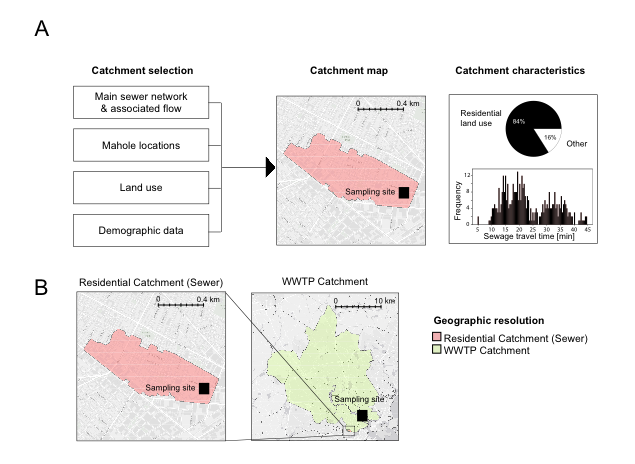
\includegraphics[width=\textwidth]{{24hr/figures/fig1_catchment_selection.png}}
    \caption{Definition and identification of residential catchments. (A). Integrating data from sewage network and flow, manhole locations, land usage, and demographic data allows for the selction of carefully curated residential manholes. (B) Upstream residential catchment vs. downstream catchment.}\label{24hr:fig1}
\end{center}
\end{figure}

\begin{figure}[h]
\begin{center}
    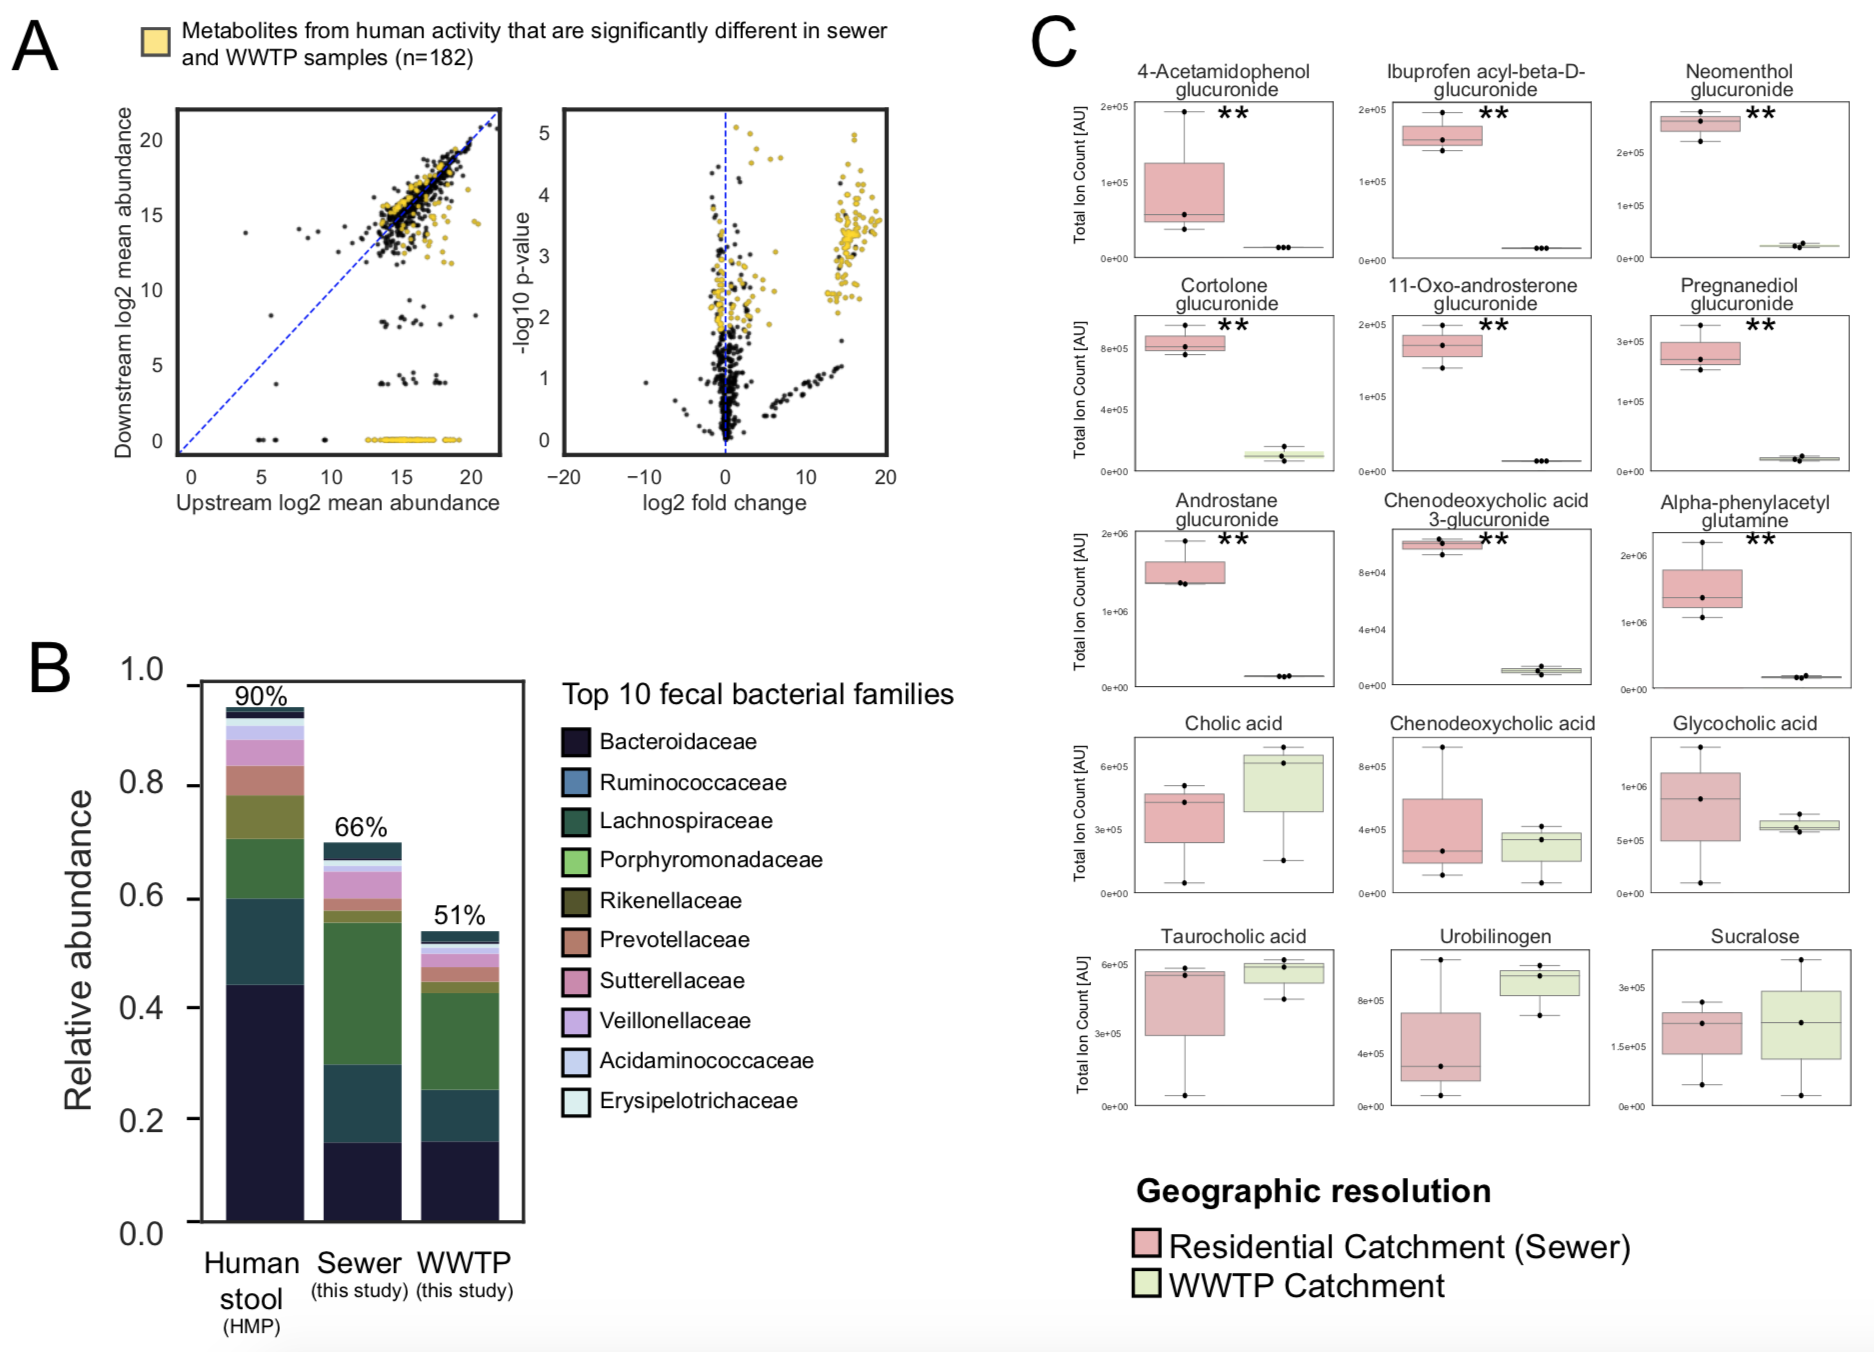
\includegraphics[width=\textwidth]{{24hr/figures/fig2_upstream_downstream.png}}
    \caption{Upstream samples find more human-derived metabolites and bacteria. (A) Abundance of metabolite features in upstream vs. downstream sample (left) and volcano plot showing fold change vs. p-value (right). (B) Residential sewage sample (``Sewer'') contains more human-associated bacteria than downstream sample (``WWTP''). (C) Abundance of various confirmed human-associated metabolites in upstream vs. downstream sample.}\label{24hr:fig2}
\end{center}
\end{figure}

\begin{figure}[h]
\begin{center}
    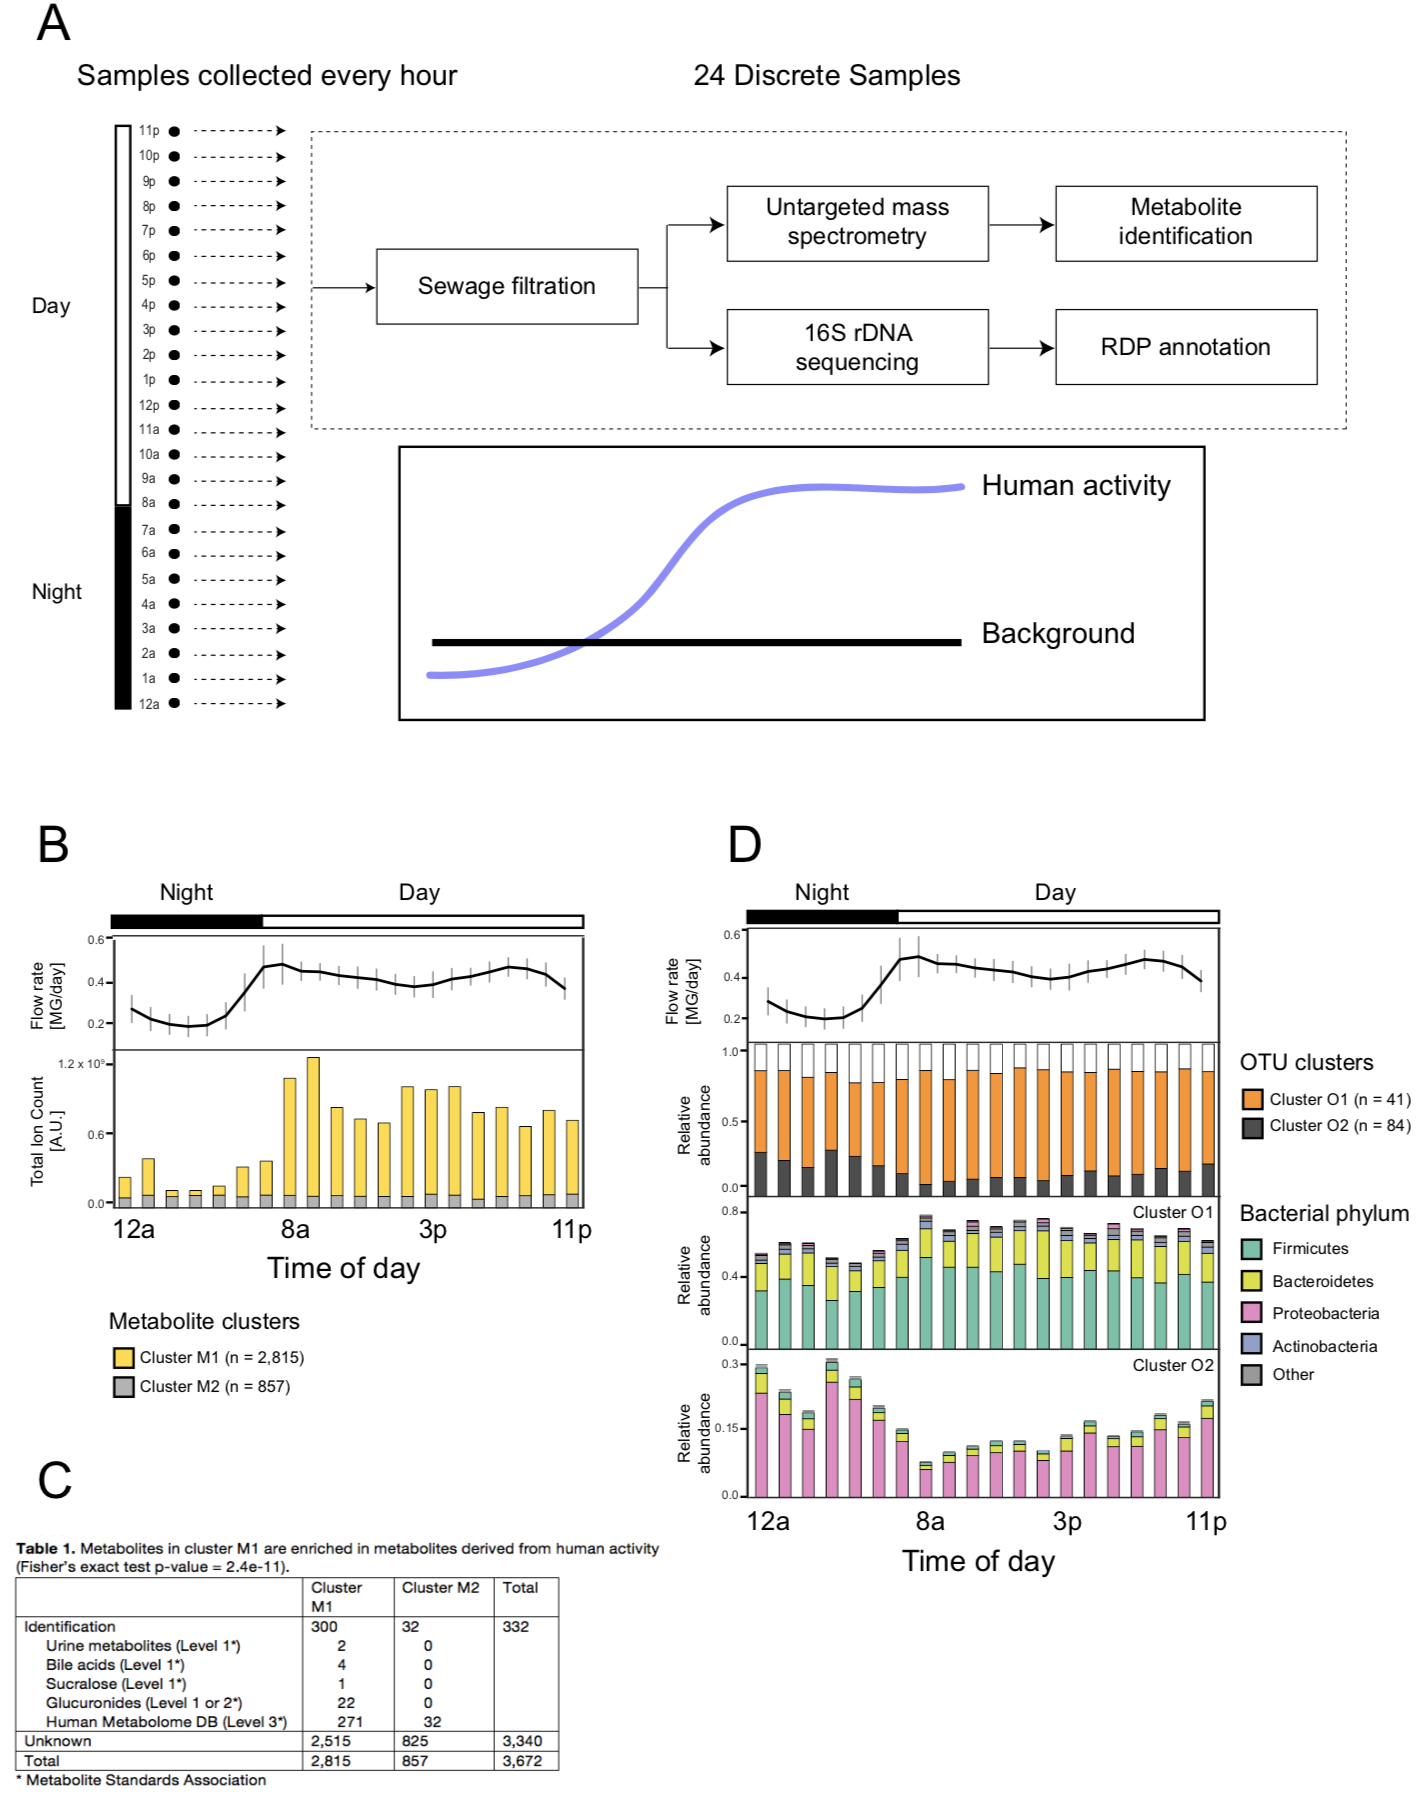
\includegraphics[width=\textwidth]{{24hr/figures/fig3_diurnal_dynamics.png}}
    \caption{Human and environmental compartments reflect human diurnal dynamics. (A) Sampling campaign and schematic of expected human activity. (B) \textit{Top}: average flow rate in residential manhole. \textit{Bottom}: total ion count of M1 and M2 metabolite clusters. (C) Number of human-associated metabolites confirmed in M1 vs. M2 clusters. (D) \textit{From top}: Average flow rate in residential manhole; relative abundance of two OTU clusters, O1 and O2; phylum-level taxonomic composition of bacterial cluster O1; phylum-level taxonomic composition of bacterial cluster O2.}\label{24hr:fig3}
\end{center}
\end{figure}

\begin{figure}[h]
\begin{center}
    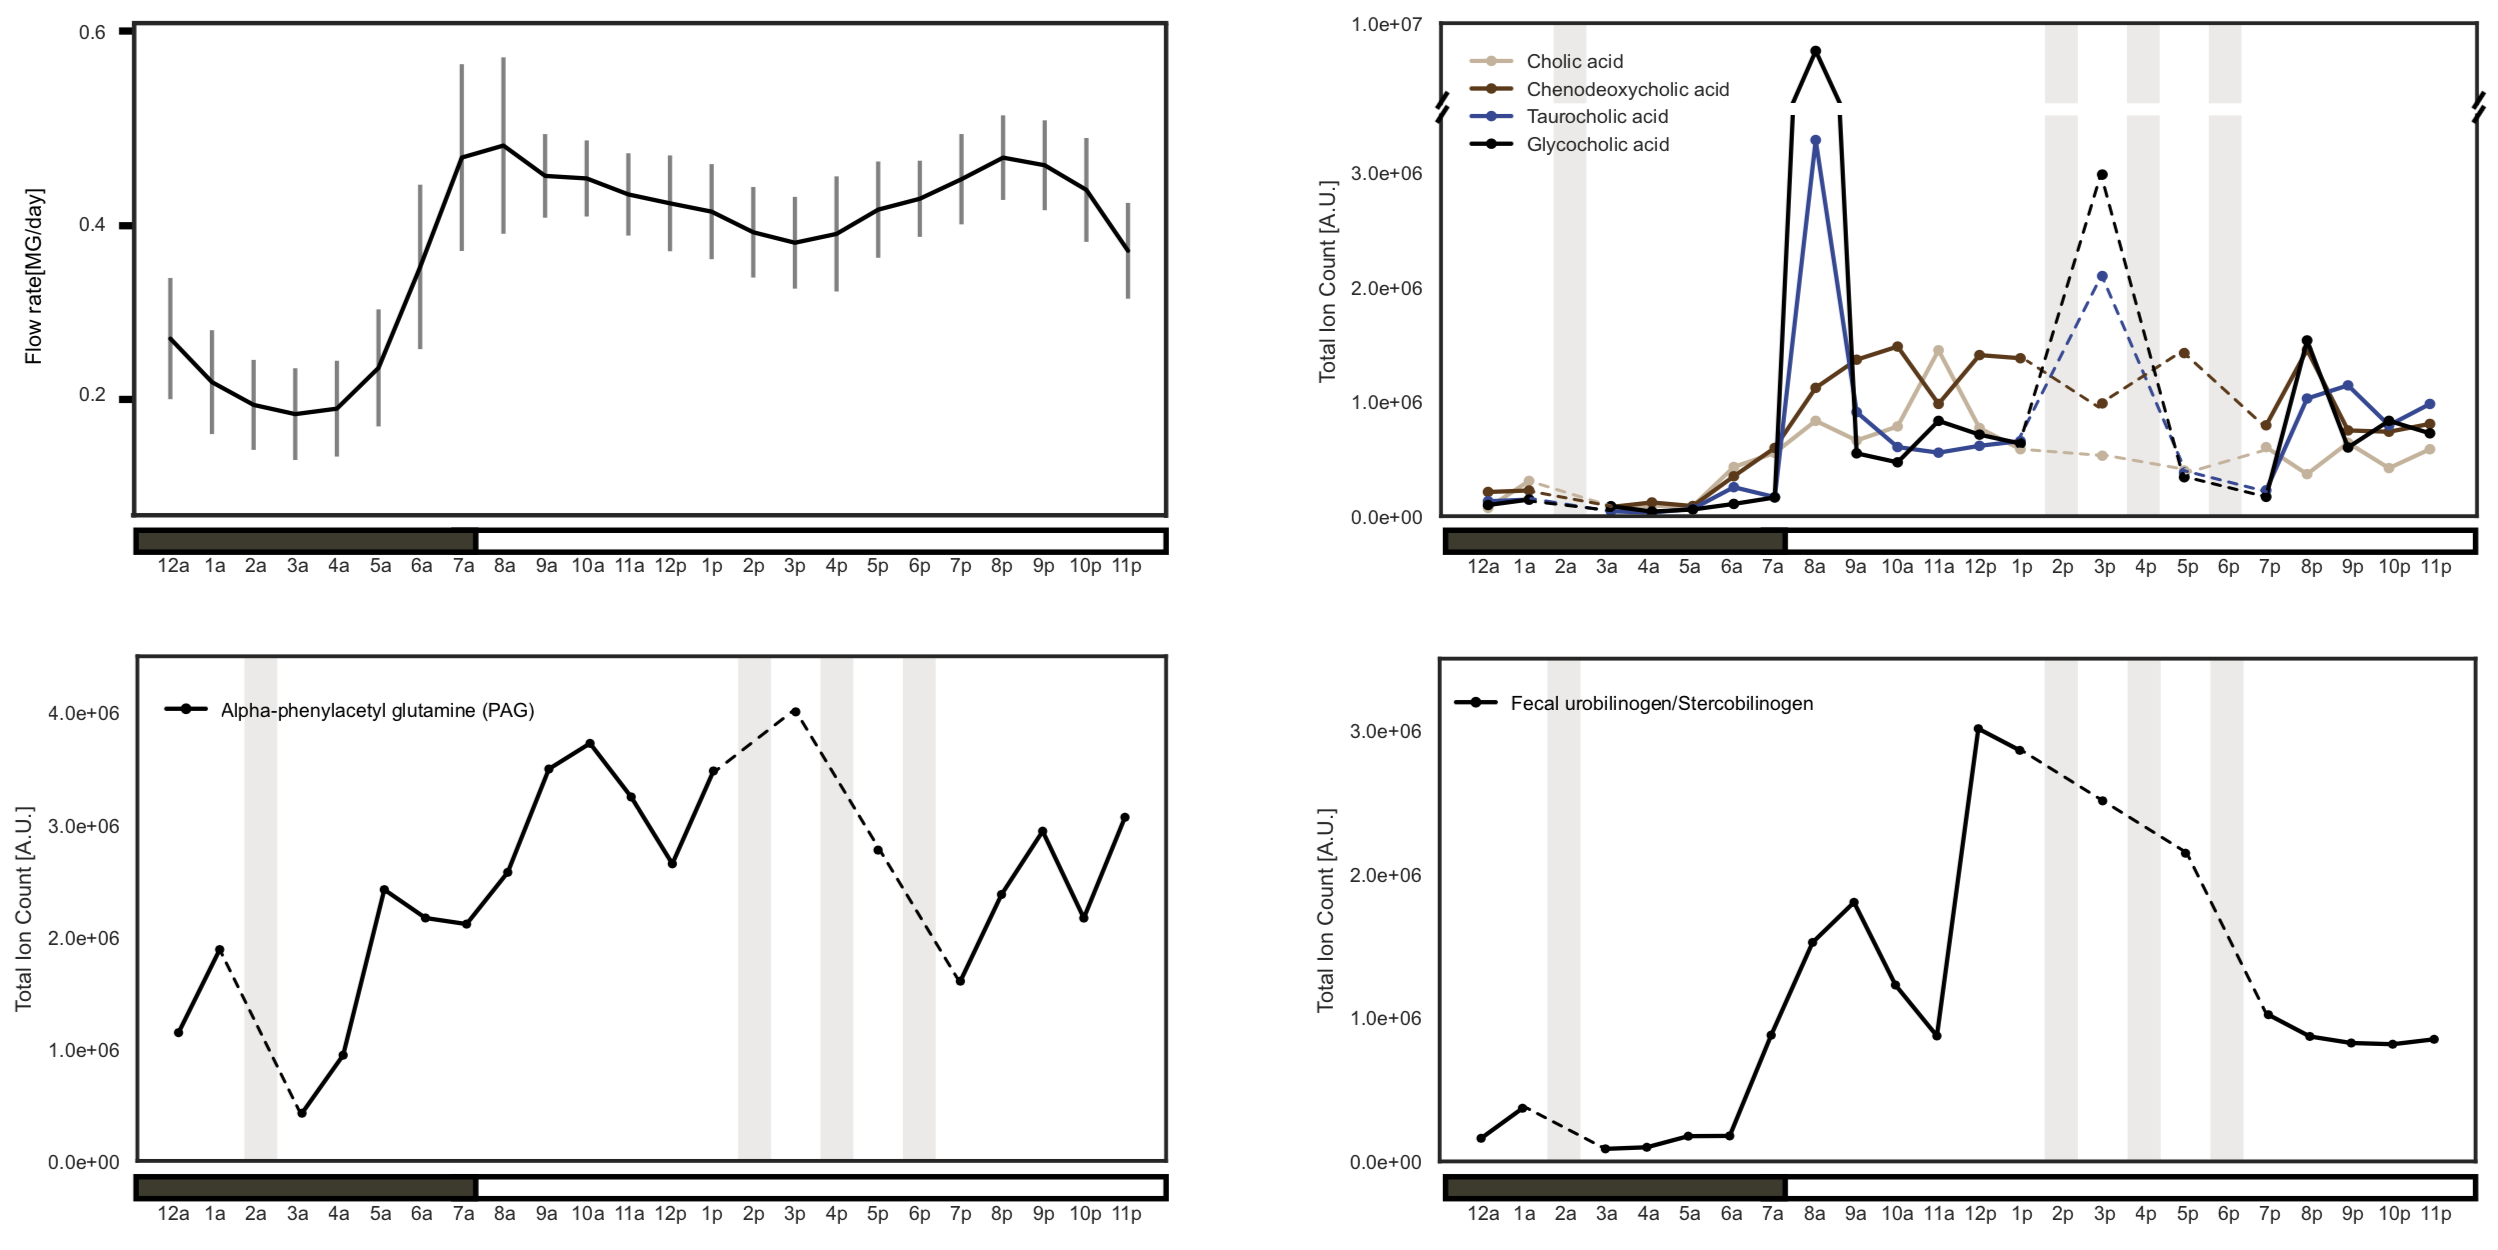
\includegraphics[width=\textwidth]{{24hr/figures/fig4_urine_fecal_markers.png}}
    \caption{Confirmed urinary and fecal biomarkers reflect human activity and behavior. (Top left) Average flow rate in residential manhole. (Bottom left) Total ion count of alpha-phenylacetylglutamine (PAG), a confirmed human urinary marker. (Top right) Total ion count of confirmed bile acids, human fecal markers. (Bottom right) Total ion count of urobilinogen, a confirmed human fecal marker. }\label{24hr:fig4}
\end{center}
\end{figure}

\begin{figure}[h]
\begin{center}
    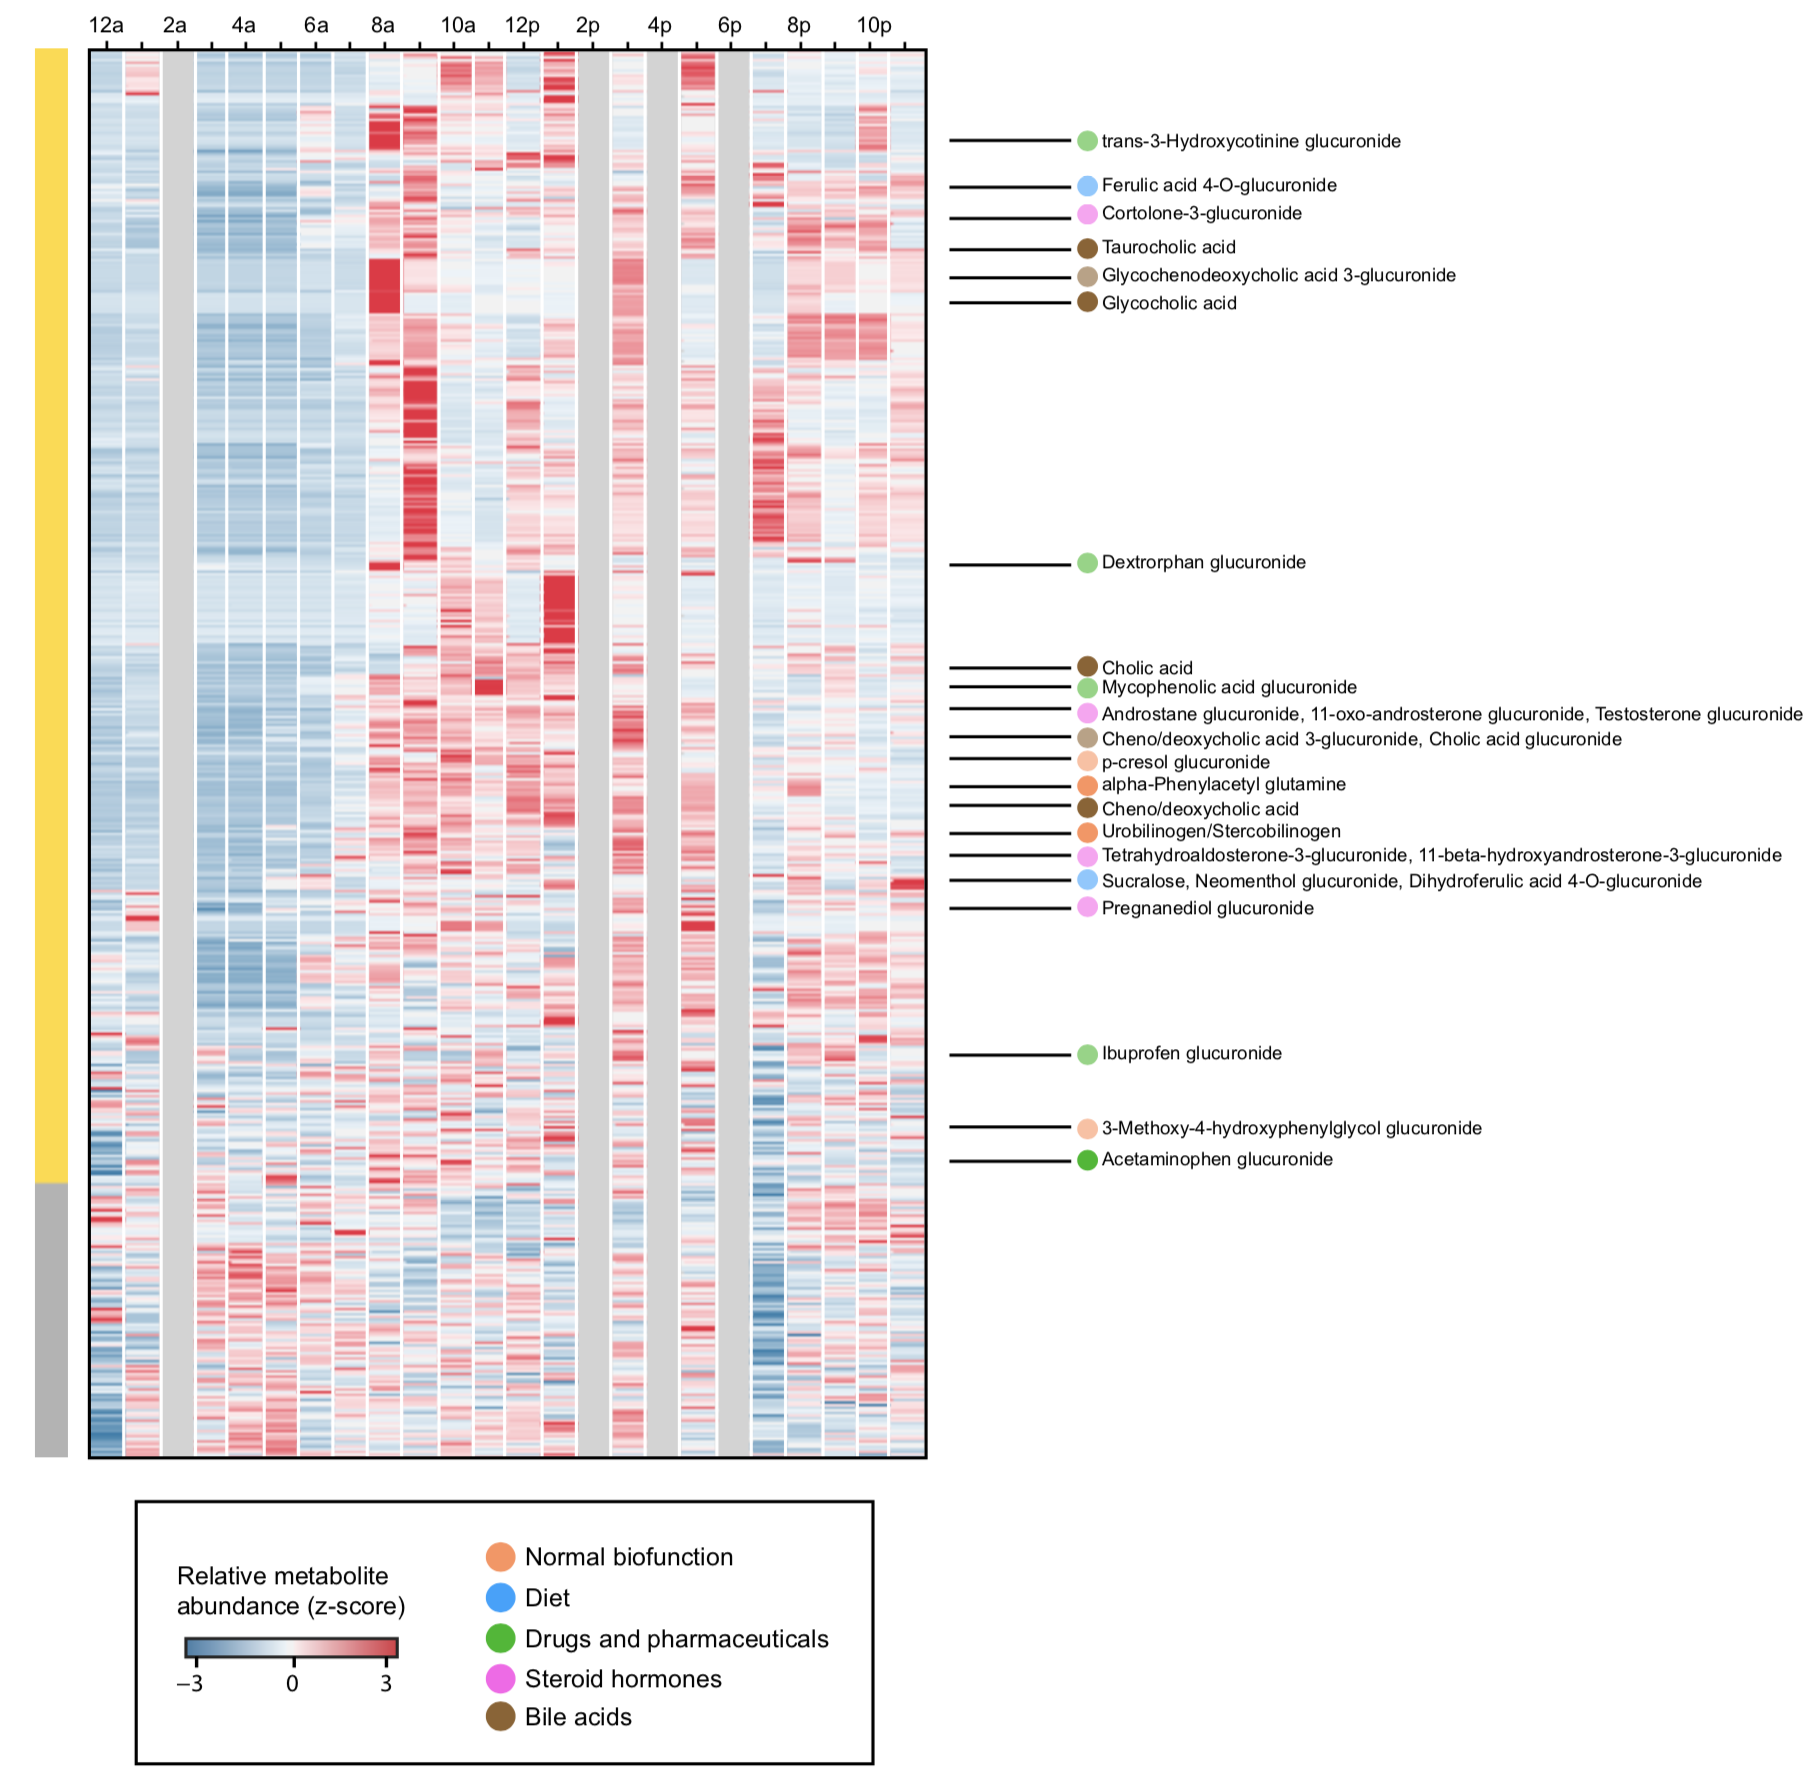
\includegraphics[width=\textwidth]{{24hr/figures/fig5_mining_big_data.png}}
    \caption{Mining untargeted data suggests identification of human health, behavioral, and lifestyle biomarkers. Heatmap of metabolite feature abundance over 24-hour samplings, with putatively identified metabolites labeled. Metabolites labeled with filled circles were confirmed with analytical standards. Labels with open circles were identified via mass-matching neutral mass with HMDB metabolites and MS2 matching.}\label{24hr:fig5}
\end{center}
\end{figure}

\begin{singlespace}
\bibliographystyle{unsrtnat}
\bibliography{24hr/24hr_refs.bib}
\end{singlespace}


%% This is an example first chapter.  You should put chapter/appendix that you
%% write into a separate file, and add a line \include{yourfilename} to
%% main.tex, where `yourfilename.tex' is the name of the chapter/appendix file.
%% You can process specific files by typing their names in at the
%% \files=
%% prompt when you run the file main.tex through LaTeX.

\chapter{Conclusions}

\section{Limitations and extensions of reported work}

In this thesis, I present multiple projects which overcome a variety of challenges to mine human microbiome data to extract clinical insights.
In the first project, I overcome the difficulty of identifying consistent biomarkers across highly variable lung and stomach communities by instead looking at the relationships between aerodigestive body sites within individual patients.
In the second project, I re-analyze gut microbiome datasets across many diseases and individual studies to identify consistent associations despite the technical challenges involved in extracting generalizable knowledge from the existing corpus of published studies.
This work motivated our development of a method to correct for batch effects presented in the third project.
In the fourth project, I present a framework to categorize disease-specific insights gleaned from previously performed analyses and experiments and leverage them to improve fecal microbiota transplant clinical trials.
Finally, in the fifth project I present preliminary results proposing residential sewage as a source of valuable public health information.
Although performed in different contexts and with different goals in mind, these computational projects share similar limitations.

\subsection{Associations not causation}

First, the findings in each project suggest associations but do not and cannot confirm causal relationships.
In Chapter \ref{chap:aspiration}, although I demonstrate that the interpretation of the aspiration-associated perturbation is consistent across a variety of analyses and metrics, such associations would still need to be recapitulated and confirmed in an independent patient cohort before being further developed as a clinical diagnostic.
Also, many more mechanistic experiments and longitudinal cohort studies would need to be done to confirm their association with subsequent aspiration-related respiratory infections.
In Chapter \ref{chap:meta-analysis}, the consistent associations that I identify across many different gut microbiome studies and microbiome-related diseases can make no claim of causality: in all case-control microbiome datasets, it is not possible to determine whether the microbiome shifts are a cause of the disease or simply responding to the host's physiological state.
In fact, finding many non-specific disease- and health-associated bacteria across these datasets suggests that a large part of these associations are more likely to be responses to the host's general health status rather than specifically causal to any given disease.
To truly find disease-associated bacteria, researchers need to identify consistent associations across multiple cohorts of their disease of interest and ensure that these associations are specific to that disease.
To develop these into disease-specific therapeutics or confirm causal associations, researchers should go further and isolate the strains of interest to test their causality in animal models.
Finally, the conceptual framework that I present in Chapter \ref{chap:donor-selection} suggests one way to advance translational microbiome science but will need to be applied in many FMT trials before its impact on FMT trial successes can be confirmed.

\subsection{Data resolution limits insights and applicability}

For the most part, these projects are anchored in the analysis of 16S rRNA data, which is more accessible than many `omics data types but comes with its own set of inherent limitations.
16S data provides a window into which bacteria are present in microbial communities but does not indicate what functions these bacteria are performing.
Because disease-mediating effects in individuals will result from bacterial function, future work should strive to incorporate function into their studies, for example by analyzing metagenomics, metabolomics or transcriptomics data, or a combination of these data types.
I hope that as datasets become more readily available, a similar cross-disease meta-analysis as Chapter \ref{chap:meta-analysis}'s will be performed, but based on metagenomics data rather than genus-level taxonomy.
I expect that a function-focused meta-analysis will find much more consistent and readily interpretable associations within studies of the same disease and across multiple diseases.

Additionally, pairing 16S analyses with functional data could ensure that the bacterial DNA detected reflect the actual bacterial communities \textit{living} in that sample.
For example, it is not known to what extent bacteria detected in human lung and stomach microbiomes are living and actively growing vs. simply a readout of DNA from dead cells.
Determining which bacteria are active in a community will be important to interpret findings and clinical interpretations from analyses of the human lung and stomach microbiomes, like the one presented in Chapter \ref{chap:aspiration}.

Another limitation of 16S data is that in most cases it cannot resolve bacteria at the strain level.
Given that different strains of the same species have dramatically different clinical presentations, this is a crucial limitation in extracting clinically relevant associations from 16S microbiome data.
The meta-analysis presented in Chapter \ref{chap:meta-analysis} was performed at the genus level so that we could compare taxa from studies which sequenced different regions of the 16S gene.
Genus-level analyses have much more limited biological interpretations than others performed at the species or strain-level.
Even with the batch correction method developed in Chapter \ref{chap:perc-norm}, meta-analyses will continue to be limited by the comparability of bacterial features between studies.
Additionally, strain-level resolution will be especially important in evaluating rational donor selection methods, where engraftment of specific donor strains may be an important factor mediating patient responses to FMT.
Finally, extending the work presented in Chapter \ref{chap:24hr} for public health applications in infectious disease surveillance will also necessarily require strain-level resolution to be useful.

\subsection{Small sample sizes limit discoveries}

Finally, these studies are limited by their sample sizes.
Although the aerodigestive cohort presented in Chapter \ref{chap:aspiration} and the meta-analysis in Chapter \ref{chap:meta-analysis} are the largest of their kind to date, the analyses that I could perform were still often limited by insufficient samples.
In Chapter \ref{chap:aspiration}, I was unable to draw robust conclusions about the relationship between reflux and the aerodigestive microbiome because the number of patients with the respective samples and metadata was too small to sufficiently power my analysis.
In fact, throughout this project I frequently found my analyses limited by the necessary confluence of samples and metadata.
For example, I would have liked to analyze the combinatorial effects of proton pump inhibitors, aspiration, and reflux on the aerodigestive microbiome, but I simply did not have enough patients with the respective samples and metadata to perform any reasonably powered analyses.

The meta-analysis presented in Chapter \ref{chap:meta-analysis} was also limited by the number of datasets and diseases.
Originally, I had hoped to compare disease-associated microbiome shifts in an unsupervised manner to identify patterns of shifts common to similar types of diseases.
For example, I wondered if I could find a consistent group of bacteria associated with inflammation across multiple inflammatory diseases.
However, I had a surprisingly difficult time finding datasets with publicly available raw data and associated patient-level clinical metadata, even given the large corpus of relevant published papers.
Thus, I did not acquire a large enough variety of diseases and datasets to enable this broader categorization of diseases and perform statistically meaningful analyses on these groups of datasets.
Future work could attempt these analyses on combined raw data, using the percentile-normalization method from Chapter \ref{chap:perc-norm} to correct for batch effects.
However, such analysis will still be constrained by the number of studies which sequenced the same region of the 16S gene, since percentile-normalized data can only be combined across features (i.e. bacterial taxa) which are common across all datasets.

One of the main conclusions of the framework presented in Chapter \ref{chap:donor-selection} is that the usual sample sizes in FMT studies will almost always limit the power of retrospective analyses to identify key bacteria.
While a tempting response to this finding might be to expand the number of FMT patients in future clinical trials, this solution will usually not be practical for multiple logistical and ethical reasons.
Unfortunately, because clinical studies are performed with human samples and sometimes require careful ethical justifications and considerable patient recruitment efforts, this challenge of small sample sizes is likely to remain an important limitation for future studies and clinical trials throughout the microbiome field.

As a pilot study evaluating the potential for residential sewage as a platform for wastewater epidemiology, the work presented in Chapter \ref{chap:24hr} had a small sample size by design.
We performed this study to determine the feasibility of mining residential sewage for public health biomarkers, and powered it accordingly.
At a broad level, the dynamics of human-associated metabolites followed the expected diurnal pattern of human activity, but any other patterns within this larger dynamic would need to be confirmed with larger studies.
We also saw significant variability between different grab samples from the upstream site, suggesting that future studies should either aggregate sampling over a longer period of time or take enough replicates to achieve statistical confidence in any measured differences.

\section{Re-analyzing existing datasets and data availability}

A core theme that has emerged from my thesis work is that re-analyzing existing microbiome datasets can add substantial value to our field.
One of my personal conclusions from the meta-analysis is that new cross-sectional gut microbiome studies should be regularly contextualized within the existing published body of work, almost as mini meta-analyses of their own.
Now that microbiome datasets are more readily available and bioinformatics tools to process and analyze them are becoming very accessible, I hope that researchers make it a habit to ask: are these associations replicated in independent patient cohorts? And: are they specific to my disease of interest or are they part of a non-specific response to health and disease?
I hope that our batch correction method can help researchers answer these questions, and that more statistical and bioinformatics tools will be developed to make meta-analyses more accessible and powerful for future researchers.

I also found the value-add of re-analyzing datasets especially relevant in microbiome research led by clinicians.
For example, the original IBD FMT trials that I re-analyzed in Chapter \ref{chap:donor-selection} did not thoroughly investigate potential donor effects on patient response in their original studies.
This is expected in part because donor heterogeneity was not usually a primary research question of interest, and also because the trials were not powered for such analyses.
However, now that multiple IBD FMT trials have been published with paired patient and donor microbiome sequencing data, hypotheses about what leads to improved patient response can be tested \textit{in silico} (as we did for butyrate producer abundance in Chapter \ref{chap:donor-selection}).
In Chapter \ref{chap:meta-analysis}, many of my datasets were pulled from studies led by clinical researchers who may not have had access to the bioinformatics and statistical expertise to fully interrogate disease associations within their datasets.
By making their data publicly available, their work continued to contribute new knowledge to the field.

Moving forward, I hope and expect that researchers continue to make their raw data publicly available and that re-analyses of such data become standard in the field.
Publicly available raw data allows researchers to ask and answer new questions, testing their hypotheses \textit{in silico} without the need for costly new studies.
New studies can also be compared with existing work to determine which of their findings hold across different studies and which are specific to their specific study.
However, using published data in new contexts comes with challenges.
As described in Chapter \ref{chap:perc-norm}, batch effects resulting from different experimental and sequencing methods can make it very difficult to compare data across different labs.
Another major challenge is data availability, and specifically clinical metadata like patient disease diagnosis.
Through this work, I have come to realize that raw data without its associated metadata is in almost all cases useless.
Given these challenges, standards for sharing data which respect patient privacy, clinicians' efforts for patient recruitment, and the needs of computational biologists will need to be agreed upon and upheld as a community.

\section{Partnerships between practitioners and computational biologists}

Throughout this thesis, I also came to appreciate the unique contributions that come from close partnerships between clinicians and computational biologists.
None of the projects in this thesis would have been possible without crucial contributions from our clinical counterparts.
Chapter \ref{chap:aspiration} was only possible because our clinical PI, Rachel Rosen, identified and framed the questions of interest in this cohort.
Then, I was able to translate her questions into computational analyses and provide preliminary answers with our data.
Working together in this way, we discovered new science and found clinically exciting results.
The meta-analysis in Chapter \ref{chap:meta-analysis} was also significantly strengthened by the inclusion of datasets which were originally purely clinical investigations, and the framework presented in Chapter \ref{chap:donor-selection} was only possible because of our lab's strong ties with the clinical experts at OpenBiome.
I hope that the future of translational microbiome research establishes structures that encourage such close collaborations.
Systems to share raw data should be designed with these collaborations in mind: the process to deposit data should be accessible to clinicians, patient information should be protected while also providing easy access to analyses that don't use the protected information, and the metadata should be curated well enough to enable straightforward analyses without much manual curation but also flexible enough to allow for the variety of study designs pursued by clinicians.

I was also especially impressed by the unique power of collaborations between scientists and practitioners through my involvement in the work presented in Chapter \ref{chap:24hr}.
That project was a result of coordination between multiple scientific disciplines as well as our city's public works and public health departments.
The urban designers on our team incorporated our computational biology perspectives into a larger vision of the future of ``smart cities.''
The public health officials we worked with helped us understand and address their practical needs, and also facilitated discussions with the community to ensure that we were being transparent and locally engaged.
Finally, our conversations with public works employees like Herbie as we stood by open manholes during our sampling campaigns gave us important insights to contextualize our experimental results and were a unique addition to my PhD experience.

\section{Finding knowledge in information}

A turning point in my thesis came when I read Gene Glass's 1976 paper coining the term ``meta-analysis'' \cite{glass-1976}.
In it, Glass argues for the underappreciated importance of consolidating and synthesizing information into knowledge, prizing work that aims to find meaning and draw conclusions from disparate existing studies.
This was a turning point in my thesis for two reasons.
First, it was the moment I became truly proud of my work, especially the meta-analysis in Chapter 3: I realized that it was not just some sort of microbiome ``stamp collection'' endeavor that anyone with basic knowledge of computational tools could do, but was instead difficult and valuable work that I had uniquely contributed to.
After reading this piece, my perspective on my thesis work changed: before, I sometimes felt that the inherent limitations of computational work meant that projects like mine were not quite as valuable as theses which develop novel experimental methods or generate new data directly testing biological hypotheses.
Now, I recognize that they are also invaluable work on their own merit.
Second, reading Glass's words helped me recognize a uniting theme in all of my work: finding the ``knowledge in the information.''
I realized that in each project presented in this thesis, I had not just mined the data to find statistical associations, but rather to interpret the associations I found and chase them all the way to their potential clinical or public health implications.
I hope that as we move forward in this exciting and vibrant field, microbiome researchers collectively become less satisfied with simply reporting new information, instead emphasizing and valuing efforts that synthesize existing knowledge and generate new insights that lead more directly to clinical impact.

\begin{singlespace}
\bibliography{chap1}
\bibliographystyle{unsrt}
\end{singlespace}

\appendix
\chapter{Supplementary Information for Chapter \ref{chap:aspiration}}\label{app:aspiration}

\graphicspath{{aspiration/figures/}}

\documentclass{article}

\usepackage[colorlinks=true]{hyperref} % for links and urls
\usepackage{amsmath,amssymb} % for math
\usepackage{color,soul} % for highlighting
\usepackage{booktabs,rotating,multirow} % for nice tables
\usepackage{authblk} % for author affiliations
\usepackage{graphicx} % for figures
\graphicspath{{../figures/}}
\usepackage[numbers]{natbib}
\usepackage[above]{placeins} % for FloatBarrier
\usepackage{amsmath} % for pretty fraction text (heatmap caption)
\usepackage{booktabs} % for multi-line table (reflux correlations)
\usepackage{lineno} % for line numbers
\usepackage{geometry} % for margins and supp fig large pages

% Rename supp figures and tables
\renewcommand{\figurename}{Supplementary Figure}
\renewcommand{\tablename}{Supplementary Table}

% Change margins
 \geometry{
 left=1.25in,
 right=1.25in,
 top=1in,
% tmargin=0.5in,
% bottom=0.5in
 }
 
 % Double-spaced
\usepackage{setspace}
\onehalfspacing


\begin{document}

%\title{The lung microbiome shifts toward the oropharyngeal microbiome in children with oropharyngeal dysphagia and aspiration}
%\title{The oropharyngeal microbiome shapes lung microbial communities in children with oropharyngeal dysphagia and aspiration}
\title{Supplemental Information for: Aerodigestive sampling reveals altered microbial exchange between lung, oropharyngeal, and gastric microbiomes in children with impaired swallow function}
\author[1,2]{Claire Duvallet}
\author[3]{Kara Larson}
\author[4]{Scott Snapper}
\author[3]{Sonia Iosim}
\author[4]{Ann Lee}
\author[4]{Katherine Freer}
\author[5]{Kara May}
\author[1,2]{Eric Alm}
\author[3,*]{Rachel Rosen}
\affil[1]{Department of Biological Engineering, MIT, Cambridge, Massachusetts}
\affil[2]{Center for Microbiome Informatics and Therapeutics, MIT, Cambridge, Massachusetts}
\affil[3]{Aerodigestive Center, Division of Gastroenterology, Hepatology and Nutrition, Boston Children's Hospital, Boston, Massachusetts}
\affil[4]{Division of Gastroenterology, Hepatology and Nutrition, Boston Children's Hospital, Boston, Massachusetts}
\affil[5]{Division of Pulmonary Medicine, Boston Children's Hospital, Boston, Massachusetts}
\affil[*]{Corresponding author}
\date{}

\maketitle


\section{Supplementary Tables and Figures}

\subsection{Supplementary Tables}

\newpage \pdfpagewidth=8.5in \pdfpageheight=16in
\FloatBarrier

\begin{table}
\begin{center}
\begin{tabular}{ccccc}  
	Family & Genus & Non-aspirator & Aspirator  & Difference \\
	\midrule
	Neisseriaceae & Neisseria & 7.1 & 41.4 & 34.2 \\ 
	Porphyromonadaceae & Porphyromonas & 28.6 & 62.1 & 33.5 \\ 
	Pasteurellaceae & Haemophilus & 50.0 & 82.8 & 32.8 \\ 
	Lachnospiraceae & Coprococcus & 10.7 & 37.9 & 27.2 \\ 
	Micrococcaceae & Rothia & 14.3 & 41.4 & 27.1 \\ 
	Prevotellaceae & Prevotella & 25.0 & 51.7 & 26.7 \\ 
	Carnobacteriaceae & Granulicatella & 32.1 & 58.6 & 26.5 \\ 
	Bacillales\_Incertae\_Sedis\_XI & Gemella & 42.9 & 69.0 & 26.1 \\ 
	Pasteurellaceae & Haemophilus & 57.1 & 82.8 & 25.6 \\ 
	Actinomycetaceae & Actinomyces & 17.9 & 41.4 & 23.5 \\ 
	Streptococcaceae & Streptococcus & 39.3 & 62.1 & 22.8 \\ 
	Lachnospiraceae & Oribacterium & 14.3 & 34.5 & 20.2 \\ 
	Leptotrichiaceae & Streptobacillus & 17.9 & 37.9 & 20.1 \\ 
	Lachnospiraceae & Lachnoanaerobaculum & 17.9 & 37.9 & 20.1 \\ 
	Fusobacteriaceae & Fusobacterium & 42.9 & 62.1 & 19.2 \\ 
	Prevotellaceae &  & 50.0 & 69.0 & 19.0 \\ 
	Flavobacteriaceae & Planobacterium & 14.3 & 31.0 & 16.7 \\ 
	Leptotrichiaceae & Leptotrichia & 14.3 & 31.0 & 16.7 \\ 
	Erysipelotrichaceae & Solobacterium & 17.9 & 34.5 & 16.6 \\ 
	Prevotellaceae & Prevotella & 21.4 & 37.9 & 16.5 \\ 
	Pasteurellaceae & Haemophilus & 28.6 & 44.8 & 16.3 \\ 
	Veillonellaceae & Veillonella & 35.7 & 51.7 & 16.0 \\ 
	Prevotellaceae &  & 46.4 & 62.1 & 15.6 \\ 
	Enterobacteriaceae & Escherichia/Shigella & 46.4 & 62.1 & 15.6 \\ 
	Neisseriaceae & Neisseria & 60.7 & 75.9 & 15.1 \\ 
	Streptococcaceae & Streptococcus & 75.0 & 89.7 & 14.7 \\ 
	Veillonellaceae & Veillonella & 35.7 & 48.3 & 12.6 \\ 
	Micrococcaceae & Rothia & 42.9 & 55.2 & 12.3 \\ 
	Streptococcaceae & Streptococcus & 42.9 & 55.2 & 12.3 \\ 
	Prevotellaceae & Prevotella & 42.9 & 55.2 & 12.3 \\ 
	Prevotellaceae & Prevotella & 64.3 & 75.9 & 11.6 \\ 
	Unknown Burkholderiales &  & 10.7 & 20.7 & 10.0 \\ 
	Bacteroidaceae & Bacteroides & 14.3 & 24.1 & 9.9 \\ 
	Porphyromonadaceae & Porphyromonas & 21.4 & 31.0 & 9.6 \\ 
	Moraxellaceae & Moraxella & 39.3 & 48.3 & 9.0 \\ 
	Prevotellaceae & Prevotella & 57.1 & 65.5 & 8.4 \\ 
	Leptotrichiaceae & Leptotrichia & 21.4 & 27.6 & 6.2 \\ 
	Fusobacteriaceae & Fusobacterium & 25.0 & 31.0 & 6.0 \\ 
	Porphyromonadaceae & Porphyromonas & 50.0 & 55.2 & 5.2 \\ 
	Neisseriaceae & Neisseria & 17.9 & 20.7 & 2.8 \\ 
	Veillonellaceae & Veillonella & 89.3 & 89.7 & 0.4 \\ 
	Unknown Bacteria &  & 21.4 & 20.7 & -0.7 \\ 
	Coriobacteriaceae & Atopobium & 21.4 & 20.7 & -0.7 \\ 
	Enterococcaceae &  & 85.7 & 82.8 & -3.0 \\ 
	Chloroplast & Streptophyta & 10.7 & 6.9 & -3.8 \\ 
	Pasteurellaceae & Haemophilus & 17.9 & 13.8 & -4.1 \\ 
	Unknown Bacillales &  & 17.9 & 13.8 & -4.1 \\ 
	Lactobacillaceae & Lactobacillus & 28.6 & 17.2 & -11.3 \\ 
	Pasteurellaceae & Haemophilus & 32.1 & 20.7 & -11.5 \\ 
	Staphylococcaceae & Staphylococcus & 60.7 & 48.3 & -12.4 \\ 
	Comamonadaceae & Acidovorax & 17.9 & 3.4 & -14.4 \\ 
	Porphyromonadaceae & Parabacteroides & 21.4 & 6.9 & -14.5 \\ 
	Comamonadaceae & Pelomonas & 21.4 & 6.9 & -14.5 \\ 
	Flavobacteriaceae & Chryseobacterium & 28.6 & 13.8 & -14.8 \\ 
	Erysipelotrichaceae & Clostridium\_XVIII & 21.4 & 3.4 & -18.0 \\ 
	Lachnospiraceae & Ruminococcus2 & 25.0 & 6.9 & -18.1 \\ 
	Flavobacteriaceae & Chryseobacterium & 50.0 & 31.0 & -19.0 \\ 
	Neisseriaceae & Microvirgula & 57.1 & 37.9 & -19.2 \\ 
	Enterobacteriaceae & Enterobacter & 82.1 & 62.1 & -20.1 \\ 
	Mycobacteriaceae & Mycobacterium & 28.6 & 6.9 & -21.7 \\ 
	Moraxellaceae & Acinetobacter & 60.7 & 37.9 & -22.8 \\ 
	Streptococcaceae & Streptococcus & 60.7 & 37.9 & -22.8 \\ 
	Bacteroidaceae & Bacteroides & 53.6 & 27.6 & -26.0 \\ 
	Unknown Bacillales &  & 57.1 & 31.0 & -26.1 \\ 
	Moraxellaceae & Acinetobacter & 60.7 & 34.5 & -26.2 \\ 
	Moraxellaceae & Enhydrobacter & 60.7 & 34.5 & -26.2 \\ 
	Lactobacillaceae & Lactobacillus & 50.0 & 20.7 & -29.3 \\ 
	Aeromonadaceae & Aeromonas & 57.1 & 27.6 & -29.6 \\ 
	Moraxellaceae & Acinetobacter & 78.6 & 41.4 & -37.2 \\ 
	Leuconostocaceae & Leuconostoc & 78.6 & 37.9 & -40.6 \\ 
	Leuconostocaceae & Weissella & 78.6 & 37.9 & -40.6 \\ 
	Moraxellaceae & Acinetobacter & 78.6 & 37.9 & -40.6 \\ 
	Streptococcaceae & Lactococcus & 78.6 & 37.9 & -40.6 \\ 
	Streptococcaceae & Lactococcus & 78.6 & 37.9 & -40.6 \\ 
	\bottomrule
\end{tabular}
\caption{Prevalence of lung-gastric fluid exchanged OTUs. Prevalence is calculated as the percentage of patients who have the OTU present in both their lungs and oropharynx, calculated separately among aspirators (N $=$ 29) and non-aspirators (N $=$ 28). OTUs are ordered by their differential prevalence in aspirators relative to non-aspirators, and are labeled with their family- and genus-level taxonomies. Blank genus names indicate OTUs which were not annotated at the genus level.}\label{tab:bal-gastric-exchanged}
\end{center}
\end{table}

\FloatBarrier
\newpage \pdfpagewidth=8.5in \pdfpageheight=11in


%% Classifiers based on abundance of exchanged OTUs
\begin{table}
\begin{center}
%\begin{tabular}{ll}

% Left table - lung-throat
\begin{tabular}{cccc}  
\textbf{Lung-oropharynx OTUs (12)} & AUC & p & N (non-asp/asp) \\
\midrule
Lung & 0.60 & 0.32 & 33/33 \\
Oropharyngeal & 0.64 & 0.13 & 43/36 \\
Both & 0.73 & 0.14 & 23/25 \\
\bottomrule
%\end{tabular}
\\
% Right table - lung-gastric
%\begin{tabular}{ccc}
\textbf{Lung-gastric OTUs (75)} &  & & \\
\midrule
Lung & 0.61 & 0.42 & 33/33 \\
Gastric fluid & 0.68 & 0.04 & 48/41 \\
Both & 0.71 & 0.07 & 28/29 \\
\bottomrule
\end{tabular}
%\end{tabular} 
\caption{\textbf{Classifiers based on the abundance of exchanged OTUs.} (Top) Classifiers built from the abundance of lung-oropharynx exchanged OTUs. (Bottom) Classifiers built from the abundance of lung-gastric exchanged OTUs. Rows indicate which microbial community was used to train each classifier. In classifiers using two sites (``Both''), abundances of each exchanged OTU in each site were considered as separate features. AUCs are calculated as the area under the average ROC curve from five-fold cross validation. Fisher's exact p values are calculated on the predictions on the hold-out data for all cross validation folds using Python's \texttt{scipy.stats.fisher\_exact} function. Each classifier was built 100 times with random patient splits and classifier initializations, and mean values are reported here. AUCs and Fisher p-values from all 100 repetitions for all classifiers are shown in Supplementary Figures \ref{fig:exchanged_cls_aucs} and \ref{fig:exchanged_cls_p}.)}\label{tab:abun-exchange-classifiers}
\end{center}
\end{table}

\newpage
\FloatBarrier

\subsection{Supplementary Figures}

% Exchange schematic
\begin{figure}[h]
        \begin{center}
        \makebox[\textwidth][c]{\includegraphics[width=\textwidth]{exchange_schematic.png}}
        \caption{Schematic illustrating an OTU which is considered exchanged between the lung and stomach (left) and one which is not (right). If an OTU is exchanged in two sites, its abundance in the two sites should be correlated across patients. Lung image was adapted from Cancer Research UK / Wikimedia Commons and the stomach image from Servier Medical Art.}
        \label{fig:exchanged_schematic}
        \end{center}
\end{figure}


% Exchanged OTUs classifiers (AUCs)
\begin{figure}[h]
        \begin{center}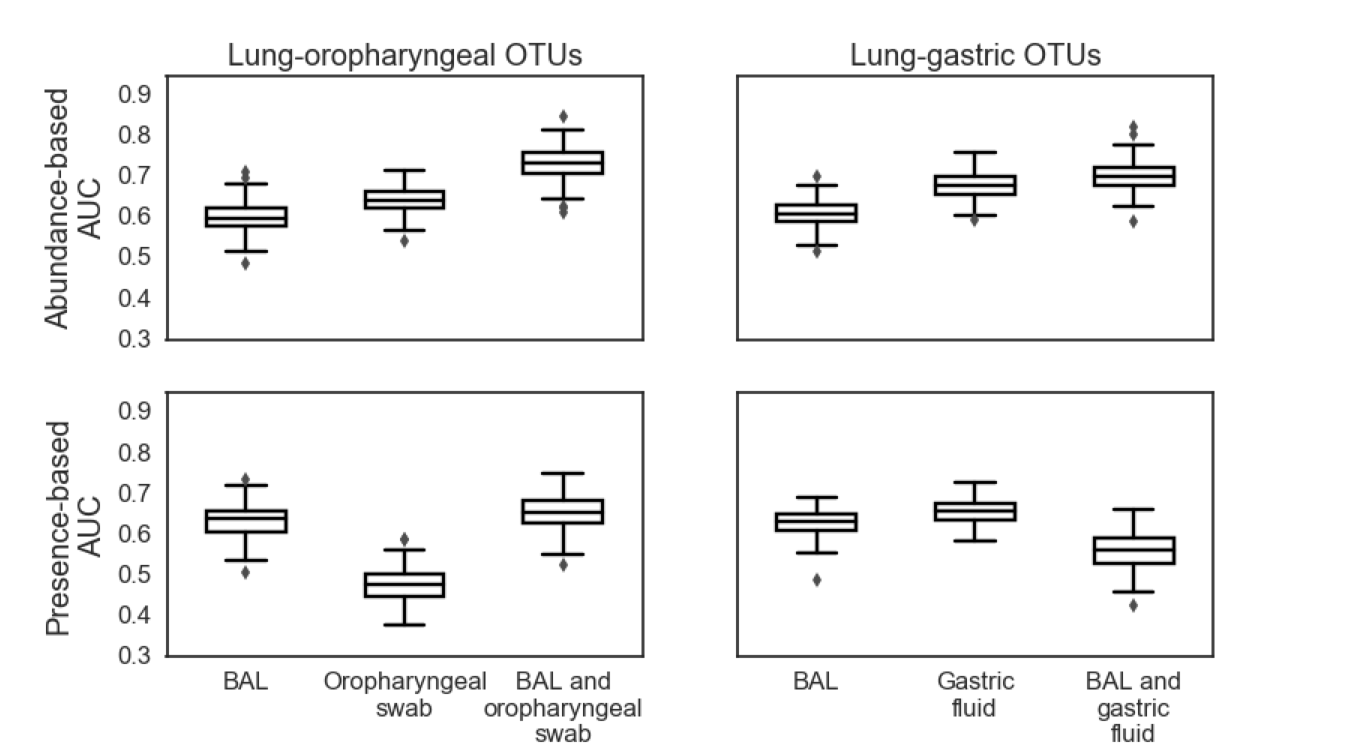
\includegraphics[width=0.8\textwidth]{asp_cls_exchanged_aucs.png}
        \caption{Areas under the ROC curve (AUC) for 100 classifiers trained on the abundance (top) or presence (bottom) of lung-oropharynx exchanged OTUs (left) or lung-gastric exchanged OTUs (right).}
        \label{fig:exchanged_cls_aucs}
        \end{center}
\end{figure}

% Exchanged OTUs classifiers (Fisher p values)
\begin{figure}[h]
        \begin{center}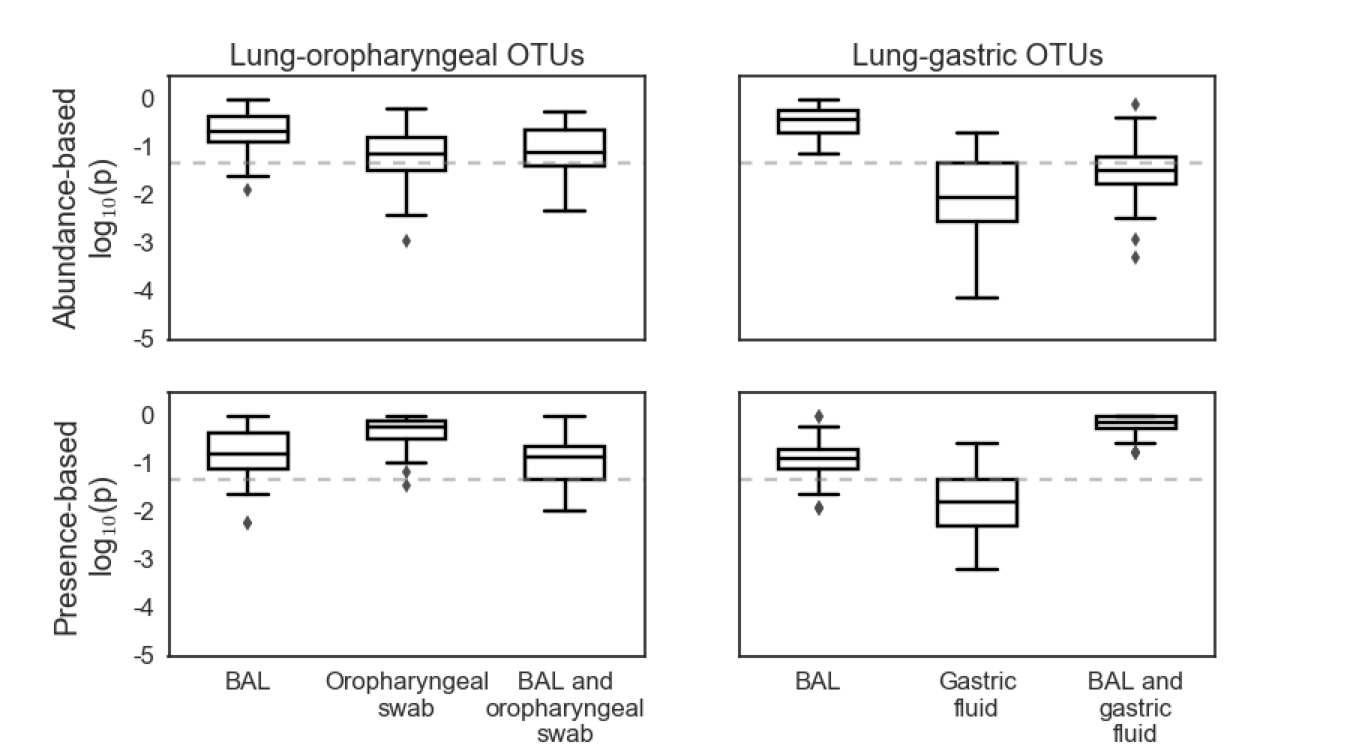
\includegraphics[width=0.8\textwidth]{asp_cls_exchanged_fisherp.png}
        \caption{Log of the Fisher p-values for 100 classifiers trained on the abundance (top) or presence (bottom) of lung-oropharynx exchanged OTUs (left) or lung-gastric exchanged OTUs (right). Dashed line indicates p $=$ 0.05.}
        \label{fig:exchanged_cls_p}
        \end{center}
\end{figure}

% Full community classifiers (AUCs and fisher p values)
\begin{figure}[h]
        \begin{center}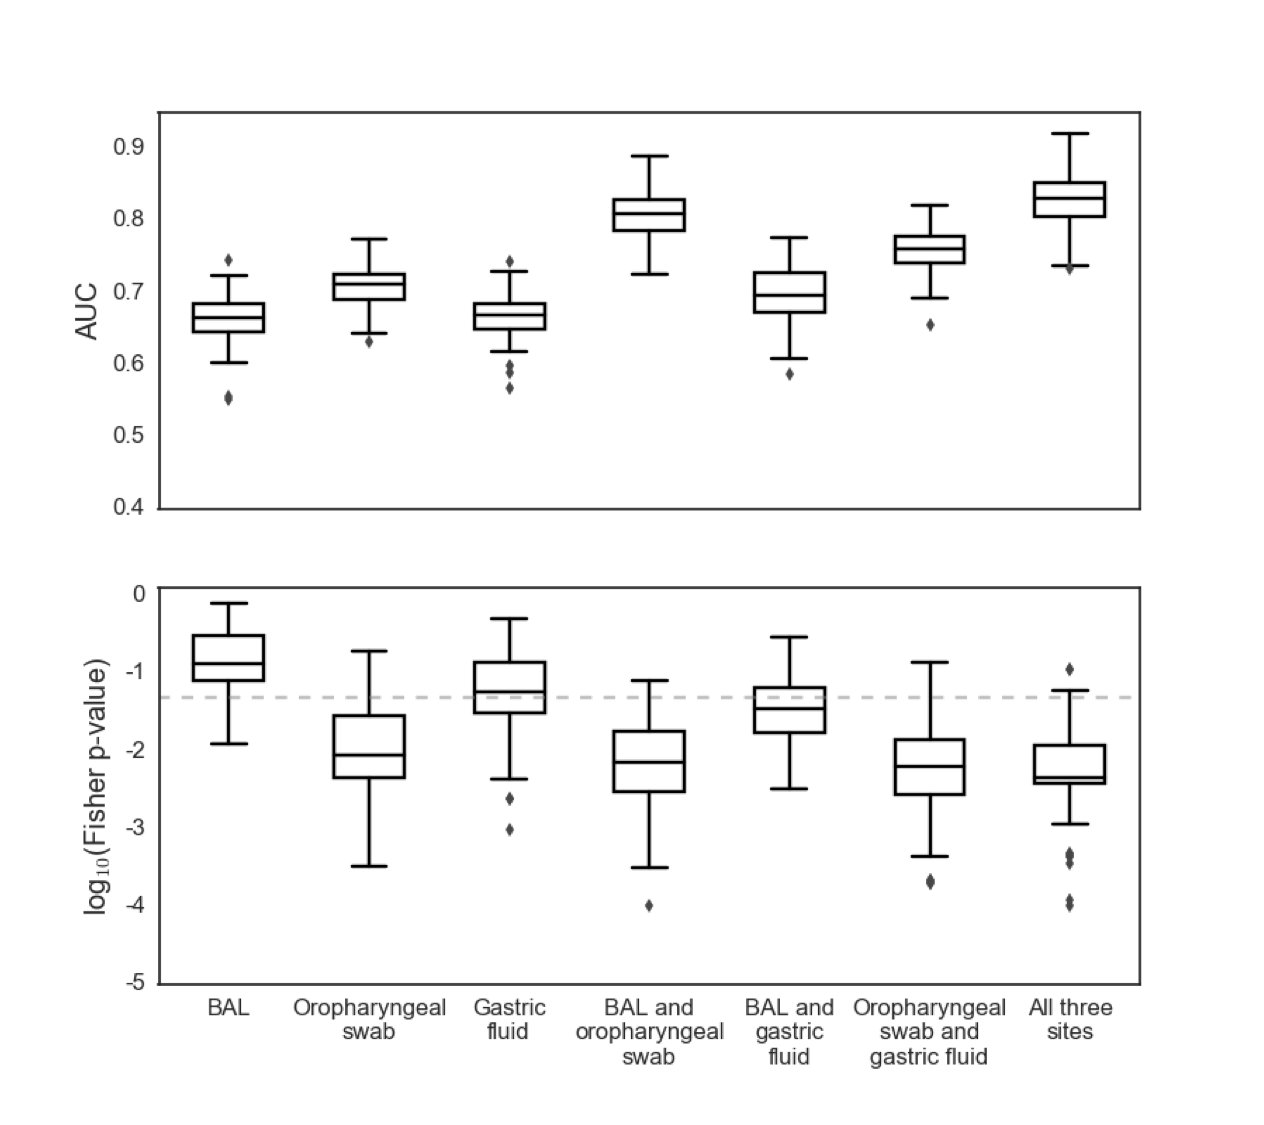
\includegraphics[width=0.8\textwidth]{asp_classifiers_aucs_fisherp.png}
        \caption{Area under the ROC curve (AUC) (top) and Fisher p-values (bottom) for 100 classifiers trained on different combinations of the full aerodigestive communities to distinguish aspirators from non-aspirators. Dashed line on the p value plot is p $=$ 0.05.}
        \label{fig:aucs_pvalues}
        \end{center}
\end{figure}

\FloatBarrier
\newpage

\end{document}

\chapter{Supplementary Information for Chapter \ref{chap:meta-analysis}}\label{app:meta-analysis}

\graphicspath{{meta-analysis/figures/}}

\section{Supplementary Notes}

\subsection{Re-processing and re-analyzing raw data yields results which are generally consistent with previously published results}\label{sec:lit_comp}

Our re-analyses of the 29 studies were largely consistent with the originally reported results, with the same taxonomic groups showing similar trends despite differences in data-processing methodologies.
We usually found fewer significant (q $<$ 0.05) differences between control and diseased groups, which is likely due to our choice of a non-parametric statistical test (Kruskall-Wallis) paired with a multi-test correction (FDR).
Thus, our results are more conservative.
We also collapsed to genus level in order to compare results across disparate studies, which prevented us from identifying species- or strain-specific associations which the original authors may have identified.
A major advantage of our re-analysis is that each data set was processed and analyzed in the same way, which allowed us to more directly compare results across studies and diseases.

\subsubsection{\textit{Clostridium difficile} Infection and enteric diarrhea are characterized by large-scale shifts in the microbiome (CDI; 4 studies)}

Schubert et al. (2014) looked at how the gut microbiota differed between CDI patients with diarrhea (n $=$ 94), non-CDI patients with diarrhea (n $=$ 89), and non-diarrheal controls (n $=$ 155) \cite{cdi-schubert}.
Similar to other CDI studies, the authors found a significant reduction in alpha diversity in patients with diarrhea (Dunn’s multiple-comparison test on AMOVA, p $<$ 0.0001).
They found that OTUs from the \textit{Ruminococcaceae}, \textit{Lachnospiraceae}, \textit{Bacteroides}, \textit{Prevotellaceae}, and \textit{Porphyromonadaceae} families were enriched in healthy subjects relative to patients with CDI and non-CDI diarrhea.
They also showed that OTUs from the \textit{Enterococcus} genus and the \textit{Enterobacteriaceae} and \textit{Erysipelotrichaceae} families were more prevalent in patients with diarrhea.
In our analysis of the data, we also observed a significant reduction in alpha diversity in patients with diarrhea (q $<=$ 0.05, KW test).
Similarly, we found that \textit{Enterobacteriaceae}, \textit{Enterococcus}, and \textit{Erysipelotrichaceae} were enriched in CDI patients, in addition to \textit{Fusobacterium}, \textit{Parvimonas}, \textit{Veillonella}, \textit{Carnobacterium}, \textit{Streptococcus}, \textit{Tetragenococcus}, \textit{Lactobacillus}, \textit{Pediococcus}, \textit{Gemella}, \textit{Staphylococcus}, \textit{Butyricicoccus}, \textit{Robinsoniella}, \textit{Clostridium XlVa}, \textit{Clostridium XlVb}, \textit{Ruminococcus2}, \textit{Flavonifractor}, \textit{Gemmiger}, \textit{Mogibacterium}, \textit{Peptostreptococcus}, \textit{Clostridium XI}, \textit{Eggerthella}, \textit{Atopobium}, \textit{Actinomyces}, \textit{Arthrobacter}, \textit{Aggregatibacter}, \textit{Pseudomonas}, and \textit{Dysgonomonas}.
As in the original study, we found that \textit{Bacteroides}, \textit{Alistipes}, \textit{Anaerovorax}, \textit{Oxalobacter}, \textit{Bordetella}, \textit{Prevotellaceae}, \textit{Porphyromonadaceae}, \textit{Lachnospiraceae}, and \textit{Ruminococcaceae} were more abundant in the healthy controls.
We also found \textit{Turicibacter}, \textit{Dialister}, \textit{Eubacterium}, \textit{Asteroleplasma}, \textit{Cloacibacillus}, \textit{Bordetella}, \textit{Oxalobacter}, \textit{Sutterella}, \textit{Parasutterella}, \textit{Desulfovibrio}, \textit{Sediminibacterium}, and \textit{Methanobrevibacter} to be enriched in the controls (q $<=$ 0.05, KW tests).
Overall, our analysis closely matched what was presented in the original manuscript.

Vincent et al. (2013) compared 25 patients with CDI to 25 healthy control patients \cite{cdi-vincent}.
The authors found a significant reduction in alpha diversity (p $<=$ 0.05, Mann-Whitney U test).
They also report a reduction in \textit{Bacteroidaceae} and \textit{Clostridiales Incertae Sedis XI} in CDI patients relative to controls, and an enrichment in \textit{Enterococcaceae} in CDI patients (p $<$ 0.05, logistic regression).
After reprocessing these data and collapsing abundances to the genus level, we observed a similar reduction in alpha diversity (q $<=$ 0.05, KW test). We saw that the \textit{Enterococcaceae} genera \textit{Enterococcus} and \textit{Proteus} were enriched in CDI patients. Healthy controls showed higher levels of \textit{Fusobacterium}, \textit{Peptoniphilus}, \textit{Murdochiella}, \textit{Anaerococcus}, \textit{Finegoldia}, \textit{Odoribacter}, \textit{Prevotella}, and \textit{Parabacteroides} relative to CDI patients. In summary, our results are fairly similar to the authors' original analysis, showing a depletion in \textit{Bacteroidetes} and an enrichment in \textit{Proteobacteria} in CDI patients.

Youngster et al. (2014) applied fecal microbiota transplants (FMTs) with materials collected from 5 healthy donors to 20 patients with recurrent \textit{Clostridium difficile} infections (CDIs) \cite{cdi-youngster}.
The goal of this study was to determine whether nasal-gastric tube or colonoscopy administration of FMTs was most effective for treating CDIs (i.e. half of the CDI patients received one or the other treatment).
The authors reported a significant reduction in alpha diversity in CDI patients vs. the healthy donors (p $<$ 0.001, Mann-Whitney test).
They did not assess whether there were significant differences in microbial community composition between CDI patients and donors, although they show that composition becomes more similar to donors following FMT.
In our analysis, we also found a significant reduction in alpha diversity (p $<=$ 0.05, KW test). \textit{Enterococcus} was enriched in CDI patients relative to healthy stool donors (q $<=$ 0.05, KW tests) and 15 genera were depleted in CDI patients relative to healthy controls.
Healthy donors were enriched in genera from \textit{Ruminococcaceae} and \textit{Lachnospiraceae} families, in addition to the genera \textit{Dialister} and \textit{Anaerosporobacter}.

Singh et al. (2015) examined differences in the gut microbiome between individuals with enteric infections (n=200) and healthy controls (n=75) \cite{edd-singh}.
The authors report a significant drop in alpha diversity in diseased patients relative to the controls (unknown test).
They also report a general reduction in the dominance of \textit{Firmicutes} and \textit{Bacteroidetes} phyla and an increase in the prevalence of \textit{Proteobacteria} in diseased patients.
Specifically, they report an increase in the abundance of \textit{Enterobacteriaceae}, \textit{Lactobacillaceae}, \textit{Pasteurellaceae}, \textit{Streptococcus}, \textit{Bacilli}, \textit{Escherichia},  \textit{Haemophilus}, and certain \textit{Ruminococcus} species in patients with diarrhea.
In healthy people, they report a significant enrichment in \textit{Verrucomicrobia}, \textit{Dorea}, \textit{Blautia}, \textit{Holdermania}, \textit{Ruminococcaceae}, \textit{Lachnospiraceae}, \textit{Butyricimonas}, \textit{Faecalibacterium}, \textit{Bacteroidaceae}, and \textit{Bifidobacterium}, \textit{Sutterella}, \textit{Parabacteroides}, \textit{Rikenellaceae}, and \textit{Oscillospira}.
After re-processing the data, we found very similar results to those originally reported.
We found that alpha diversity was significantly lower in patients with enteric infections (q $<=$ 0.05, KW test).
We saw significant enrichment in \textit{Proteobacteria} families in patients with diarrhea, including \textit{Enterobacteriaceae}, \textit{Pasteurellaceae}, \textit{Campylobacteraceae}, and \textit{Neisseriaceae}.
We also saw higher levels of \textit{Fusobacterium}, \textit{Parvimonas}, \textit{Veillonella}, \textit{Lactococcus}, \textit{Streptococcus}, \textit{Enterococcus}, \textit{Tetragenococcus}, \textit{Gemella}, \textit{Ruminococcus II}, \textit{Peptostreptococcus}, and \textit{Collinsella} in diseased patients.
In the healthy controls, we found enrichment of 43 genera, including \textit{Sutterella}, \textit{Verrucomicrobia} (\textit{Akkermansia}), \textit{Ruminococcaceae}, \textit{Lachnospiraceae}, \textit{Bacteroidaceae}, and \textit{Bifidobacterium}.
In addition, we saw higher levels of several members of \textit{Rumminococcaceae}, \textit{Lachnospiraceae}, and \textit{Bacteroidales} in healthy controls (q $<=$ 0.05, KW tests).
Overall, our results largely overlap with those presented, but we identify a number of significant taxa that were not originally reported.

Taken together, we see large-scale shifts in the microbiome associated with both CDI and non-CDI diarrhea.
The dysbiosis of enteric infection and diarrhea is quite consistent across studies.
In general, \textit{Proteobacteria} increase in prevalence in patients with diarrhea, with a concomitant decrease in \textit{Bacteroidetes} and \textit{Firmicutes}.
In particular, we see a reduction in butyrate-producing Clostridia, including genera within \textit{Ruminococcaceae} and \textit{Lachnospiraceae} families, which have been associated with a healthy gut.
We also see in increase in prevalence of organisms often associated with lower pH and higher oxygen levels of the upper-gut, like \textit{Lactobacillaceae} and \textit{Enterobacteriaceae} \cite{donaldson2016gut}, in patients with diarrhea.
Thus, diarrhea leads to consistent and large-scale rearrangements in the composition of the gut microbiome.

\subsubsection{Colorectal Cancer has a consistent, ootentially pathogenic microbial signature (CRC; 4 studies)}

Baxter et al. (2016) looked at differences in the microbiomes of 120 colorectal cancer (CRC) patients, 198 patients with non-cancerous adenomas, and 172 healthy controls \cite{crc-baxter}.
Similar to prior work, the authors found that \textit{Porphyromonas}, \textit{Peptostreptococcus}, \textit{Parvimonas}, and \textit{Fusobacterium} were positively associated with CRC (random forest classifiers).
Furthermore, they found that the absence of certain \textit{Lachnospiraceae} species was associated with the presence of adenomas.
We found similar patterns in our re-analysis of these data, with \textit{Fusobacterium}, \textit{Peptostreptococcus}, \textit{Parvimonas}, and \textit{Porphyromonas} enriched in CRC patients (q $<=$ 0.05, KW tests).
We also found higher levels of \textit{Victivallis}, \textit{Peptoniphilus}, \textit{Anaerococcus}, \textit{Catenibacterium}, \textit{Staphylococcus}, \textit{Collinsella}, \textit{Enterobacter}, and \textit{Alloprevotella} in CRC patients (q $<=$ 0.05, KW tests).
We found that healthy controls were enriched in \textit{Lachnobacterium} (genus within \textit{Lachnospiraceae}), \textit{Gemmiger} (within \textit{Rumminococcaceae}), \textit{Clostridium XVIII}, and \textit{Haemophilus} (q $<=$ 0.05, KW tests).
Overall, these results match what has been reported previously for CRC \cite{brennan2016gut}.

Zeller et al. (2014) collected microbiome data from 41 CRC patients and 75 control patients \cite{crc-zeller}.
At the phylum level, they found that \textit{Proteobacteria}, \textit{Fusobacteria}, and \textit{Bacteroidetes}, were more abundant in CRC patients, while \textit{Firmicutes} and \textit{Actinobacteria} were enriched in control patients.
At the genus level, the authors report higher levels of \textit{Fusobacterium}, \textit{Pseudoflavonifractor}, \textit{Peptostreptococcus}, \textit{Leptotrichia}, \textit{Porphyromonas}, \textit{Desulfovibrio}, \textit{Parvimonas}, \textit{Selenomonas}, and \textit{Bilophila} in CRC patients (q $<=$ 0.1, FDR-corrected Wilcoxon tests).
Healthy controls were enriched in \textit{Bifidobacterium}, \textit{Acinetobacter}, \textit{Campylobacter}, \textit{Ruminococcus}, and \textit{Eubacterium} genera (q $<=$ 0.1, FDR-corrected Wilcoxon tests).
In our re-analysis we found enrichment of \textit{Fusobacterium}, \textit{Parvimonas}, \textit{Flavonifractor}, \textit{Anaerotruncus}, \textit{Anaerovorax}, \textit{Peptostreptococcus}, \textit{Comamonas}, \textit{Eikenella}, \textit{Butyricimonas}, and \textit{Porphyromonas} genera in CRC patients (q $<=$ 0.05, KW tests).
In healthy patients, we found higher levels of \textit{Anaerostipes} (within \textit{Lachnospiraceae}; q $<=$ 0.05, KW tests).

Wang et al. (2011) analyzed a cohort of 46 CRC patients and 56 healthy controls \cite{crc-zhao}.
The authors found no difference in alpha diversity between CRC and control patients.
CRC patients had higher abundances of \textit{Porphyromonas}, \textit{Escherichia-Shigella}, \textit{Enterococcus}, \textit{Streptococcus}, and \textit{Peptostreptococcus} genera (p $<=$ 0.05, Mann-Whitney).
The authors report that healthy controls were enriched \textit{Bacteroides}, \textit{Roseburia}, \textit{Alistipes}, \textit{Eubacterium}, and \textit{Parasutterella} genera (p $<=$ 0.05, Mann-Whitney).
We found very similar results in our re-analysis of these data.
We saw greater levels of \textit{Enterococcus}, \textit{Peptostreptococcus}, \textit{Enterobacter}, \textit{Klebsiella}, \textit{Escherichia-Shigella}, and \textit{Porphyromonas} genera in CRC patients (q $<=$ 0.05, KW tests).
And we observed significantly higher levels of \textit{Bacteroides}, and several genera within \textit{Lachnospiraceae} in healthy controls (q $<=$ 0.05, KW tests).
Furthermore, we also did not detect any significant differences in alpha diversity between CRC and healthy patients.

Chen et al. (2012) analyzed stool from 22 healthy patients and 21 CRC patients \cite{crc-xiang}.
The authors found that \textit{Paraprevotella}, \textit{Eubacterium}, \textit{Desulfovibrio}, \textit{Mogibacterium}, \textit{Collinsella}, \textit{Anaerotruncus}, \textit{Slackia}, \textit{Anaerococcus}, \textit{Porphyromonas}, \textit{Fusobacterium}, and \textit{Peptostreptococcus} genera were significantly enriched in CRC patients relative to controls, while \textit{Bifidobacterium}, \textit{Faecalibacterium}, and \textit{Blautia} were reduced in CRC patients (p $<=$ 0.05, Mann-Whitney).
In our re-analysis of this data set, we found no significant differences between CRC and control patients.
Again, this is likely due to the small number of replicates and our implementation of multiple-test corrections.
However, non-significant trends were largely in agreement with the original results.

Across these four colorectal cancer studies, we find significant agreement.
Dysbiosis associated with CRC is generally characterized by increased prevalence of \textit{Fusobacterium}, \textit{Porphyromonas}, \textit{Peptostreptococcus}, \textit{Parvimonas}, \textit{Leptotrichia}, \textit{Desulfovibrio}, and \textit{Anaerococcus} genera (i.e. these genera were higher in CRC patients in 2 or more studies).
In addition, there is a consistent decrease in the abundances of \textit{Faecalibacterium}, \textit{Blautia}, \textit{Bacteroides} genera and organisms from the \textit{Lachnospiraceae} family in CRC patients.
CRC appears to have a smaller impact on overall community structure than diahrrea.
Indeed, we saw no significant differences in alpha diversity between healthy controls and CRC patients.
In summary, CRC is characterized by a consistent enrichment of disease-associated bacteria.

\subsubsection{Inflammatory Bowel Disease is characterized by a depletion of health-associated bacteria (IBD - Ulcerative Colitis and Crohn's Disease; 4 studies)}

Gevers et al. (2014) looked for microbial signatures of Crohn's disease (CD) samples across 447 CD patients and 221 non-IBD controls \cite{ibd-gevers}.
Non-IBD controls were patients with non-inflammatory conditions such as abdominal pain and diarrhea.
The authors report increased abundance of \textit{Enterobacteriaceae}, \textit{Pasteurellaceae}, \textit{Veillonellaceae}, and \textit{Fusobacteriaceae} in CD patients.
CD patients also showed a drop in the abundances of \textit{Erysipelotrichales}, \textit{Bacteroidales}, and \textit{Clostridiales} (\textit{Ruminococcaceae} and \textit{Lachnospiraceae}) taxa.
These results were based on a mixture of 16S amplicon and shotgun metagenomic sequencing.
In our re-analysis of the 16S stool data, we found significant enrichment in \textit{Anaerosporobacter}, \textit{Roseburia}, \textit{Hespellia}, \textit{Ruminococcus II}, \textit{Eubacterium}, \textit{Pseudoflavonifractor}, \textit{Sporobacter}, \textit{Ruminococcus}, \textit{Subdoligranulum}, \textit{Papillibacter}, \textit{Collinsella}, and \textit{Methanobrevibacter} in healthy patients (q $<=$ 0.05, KW tests).
The only genera that we saw significantly enriched in CD patients were \textit{Lactobacillus} and \textit{Acetanaerobacterium} (q $<=$ 0.05, KW tests).
We found a similar set of taxa enriched in the controls, but did not detect as many significant CD-enriched genera as the authors reported.
This is likely due to the fact that we restricted our analysis to the 16S stool data.
However, we saw non-significant trends in \textit{Enterobacteriaceae} and \textit{Veillonellaceae} consistent with the results reported in the original paper.

Morgan et al. (2012) studied a cohort of 119 CD patients, 74 UC patients, and 27 healthy controls \cite{ibd-hut}.
The authors found that healthy patients’ gut microbiomes were significantly enriched in \textit{Roseburia}, \textit{Phascolarctobacterium}, and an unclassified genus in the family \textit{Veillonellaceae} (multivariate linear model, q $<=$ 0.25).
Patients with UC showed significantly higher levels of \textit{Clostridiaceae} (multivariate linear model, q $<=$ 0.25).
In our re-analysis, we did not find any genera that were significantly enriched in IBD patients.
We found that healthy patients had significantly greater abundances of \textit{Ruminococcus}, and \textit{Gemmiger} relative to both UC and CD patients (q $<=$ 0.05, KW tests).
Additionally, CD patients were depleted in \textit{Clostridium IV} relative to healthy controls (q $<=$ 0.05, KW tests).

Papa et al. (2012) studied a cohort of 23 CD patients, 43 UC patients, and 24 non-IBD controls \cite{ibd-papa}.
Non-IBD controls were patients with symptoms such as: constipation, abdominal pain, gastroesophageal reflux, poor weight gain, diarrhea, blood in stool and oropharyngeal dysphagia.
At the genus level, they found that controls were enriched in \textit{Alistipes}, \textit{Subdoligranulum}, \textit{Anaerovorax}, \textit{Oscillibacter}, \textit{Parabacteroides}, \textit{Odoribacter}, \textit{Ruminococcus}, \textit{Butyricicoccus}, \textit{Akkermansia}, \textit{Anaerotruncus}, \textit{Sporobacter}, \textit{Phascolarctobacterium}, \textit{Lawsonia}, \textit{Ethanoligenens}, \textit{Peptococcus} relative to IBD patients (KW, q $<$ 0.01).
The only genus that was found to be enriched in IBD patients was \textit{Escherichia-Shigella}.
In our re-analysis, we also found \textit{Escherichia-Shigella} and \textit{Cronobacter} to be enriched in patients with IBD (q $<=$ 0.05, KW tests).
When comparing healthy controls with UC patients, we also found an enrichment of \textit{Haemophilus} in the UC patients.
Control patients showed higher abundances of \textit{Phascolarctobacterium}, \textit{Butyricicoccus}, \textit{Ruminococcus II}, \textit{Oscillibacter}, \textit{Ruminococcus}, \textit{Gemmiger}, \textit{Subdoligranulum}, \textit{Clostridium IV}, \textit{Odoribacter}, \textit{Alistipes}, and \textit{Parabacteroides} relative to all IBD patients (q $<=$ 0.05, KW tests).
Additionally, control patients were enriched in \textit{Clostridium XIVa}, \textit{Flavonifractor}, and \textit{Akkermansia} relative to UC patients.
Overall, our results match very closely what was found in the original paper.

Willing et al. (2010) compared 29 CD patients and 16 UC patients to 35 healthy controls \cite{ibd-engstrand}.
The authors reported variable, and sometimes opposing shifts in the microbiomes of patients with UC, ileal CD and colonic CD at different taxonomic resolutions.
We found no significant differences between IBD and healthy patients in our re-analysis.
When comparing healthy controls with CD cases only, we found an enrichment of \textit{Butyricicoccus} and \textit{Oscillibacter} in the control patients (q $<=$ 0.05, KW tests).

In summary, there are certain consistencies across IBD studies.
IBD patients tend to be depleted in butyrate-producing clostridia: \textit{Ruminococcus} and \textit{Lachnospiraceae}.
The organisms the are enriched in CD and UC patients tend to vary across studies.
One consistency is organisms associated with the upper gut, like \textit{Lactobacillus} and \textit{Enterobacteriaceae} appear to be enriched in IBD patients \cite{donaldson2016gut}.
This result fits with the reduced stool transit times associated with IBD (i.e. diarrhea).

\subsubsection{Obesity shows a somewhat inconsistent microbial signature (OB; 5 studies)}

Goodrich et al. (2014) studied a cohort of 416 twin pairs: 422 normal BMI, 322 overweight, and 185 obese \cite{ob-goodrich}.
The authors report higher levels of \textit{Lactobacillaceae}, \textit{Eggerthella}, and \textit{Lachnospiraceae} (\textit{Blautia} and \textit{Dorea}) in obese individuals (q $<$ 0.05, FDR-corrected T-test).
They showed enrichment for \textit{Christensenellaceae}, \textit{Dehalobacterium}, \textit{Lachnospira}, \textit{Mogibacteriaceae}, \textit{Rikenellaceae}, \textit{Methanobre}, \textit{Coriobacteriaceae}, \textit{Peptococcaceae}, \textit{Oscillospira}, \textit{Ruminococcaceae}, and \textit{Sarcina} in healthy BMI individuals (q $<$ 0.05, FDR-corrected T-test).
In our re-analysis, we found higher levels of \textit{Streptococcus}, \textit{Weissella}, \textit{Roseburia}, \textit{Blautia}, \textit{Clostridium XlVb}, and \textit{Mogibacterium} in obese individuals, while \textit{Robinsoniella}, \textit{Ruminococcaceae} (\textit{Oscillibacter}, \textit{Pseudoflavonifractor}, \textit{Sporobacter}, and \textit{Anaerofilum}), and \textit{Anaerovorax} were more abundant in low-BMI individuals (q $<=$ 0.05, KW tests).
Our results only partially agree with the authors' original findings, which may be due to the fact that we used a different statistical test and OTU-calling method and that we binned the data at the genus level.

Zupancic et al. (2012) analyzed 310 individuals from an Amish population with varying BMIs \cite{ob-zupancic}.
They found a significant positive correlation between the abundance of \textit{Collinsella} and BMI (i.e. enriched in obese individuals), while \textit{Lachnobacterium}, \textit{Anaerotruncus}, \textit{Faecalibacterium}, and \textit{Clostridium} were negatively correlated with BMI (i.e. enriched lean individuals) (p < 0.001, Spearman correlation).
We found no significant differences in the proportion of genera between lean and obese individuals in our re-analysis.

Turnbaugh et al. (2008) looked differences in gut microbial community structure between 31 monozygotic and 23 dizygotic twin pairs concordant for leanness or obesity \cite{ob-gordon}.
The authors report a reduction in alpha diversity in obese individuals.
They also report a significant decrease in \textit{Bacteroidetes}  and an increase in \textit{Actinobacteria} in obese twins.
In our re-analysis of these data, we did not see a significant reduction in alpha diversity (Supplementary Figure \ref{fig:fig_alpha}).
We found significant increases in \textit{Catenibacterium}, \textit{Acidaminococcus}, \textit{Megasphaera}, \textit{Lactobacillus}, \textit{Roseburia}, and \textit{Collinsella} in obese twins (q $<=$ 0.05, KW tests).
\textit{Coprobacillus}, \textit{Clostridium XVIII}, \textit{Phascolarctobacterium}, \textit{Clostridium XlVb}, \textit{Oscillibacter}, \textit{Flavonifractor}, \textit{Pseudoflavonifractor}, \textit{Ruminococcus}, \textit{Clostridium IV}, \textit{Gordonibacter}, \textit{Alistipes}, and \textit{Barnesiella} were significantly enriched in lean twins (q $<=$ 0.05, KW tests).

Ross et al. (2015) looked at 63 Mexican American patients with varying BMIs \cite{ob-ross}.
They found no significant differences between patients with high and low BMIs within their 63 patient cohort, but identified several significant differences between their patient population and the HMP data set.
However, it is unclear whether these differences were related to obesity, so we do not discuss them here.
Our re-analysis of these results also found no significant differences in the relative abundances of bacterial genera between high- and low-BMI subjects.

Zhu et al. (2013) compared across a cohort of 16 healthy and 25 obese patients, in addition to 22 patients with Nonalcoholic steatohepatitis (see below) \cite{nash-baker}.
For obesity, the authors found that \textit{Prevotella} was enriched in high-BMI patients, while healthy controls showed significantly greater relative abundances of \textit{Bifidobacterium}, \textit{Blautia}, and \textit{Faecalibacterium} (p $<=$ 0.05, ANOVA with post-hoc Tukey's tests).
In our re-analysis of these data, we found a significant enrichment of \textit{Peptoniphilus}, \textit{Anaerococcus}, \textit{Finegoldia}, \textit{Leuconostoc}, \textit{Mogibacterium}, \textit{Varibaculum}, \textit{Campylobacter}, \textit{Prevotella}, and \textit{Porphyromonas} in obese patients (q $<=$ 0.05). Healthy patients were significantly enriched in \textit{Akkermansia}, \textit{Murdochiella}, \textit{Blautia}, \textit{Lachnospiracea incertae sedis}, and \textit{Clostridium IV}, \textit{Anaerovorax} (q $<=$ 0.05, KW tests).

Overall, we found several differences between lean and obese patients that were consistent across at least two studies.
\textit{Roseburia} and \textit{Mogibacterium} were enriched in obese individuals in more than one study. \textit{Pseudoflavonifractor}, \textit{Oscillobacter}, \textit{Anaerovorax} and \textit{Clostridium IV} were enriched in the controls across more than one study. However, no genera showed consistent differences across three or more studies.
Our results are largely consistent with a recent meta-analysis of obesity studies, which found no universal signature of human obesity \cite{Sze07092016}.

\subsubsection{Human Immunodeficiency Virus microbial signature is confounded with patient cohorts (HIV; 3 studies)}

Dinh et al. (2015) compared the gut microbiome from 16 healthy patients to 22 patients with chronic HIV infections \cite{hiv-dinh}.
The authors report an general enrichment in \textit{Proteobacteria} in HIV-infected patients.
At the genus level, they found a significant enrichment in \textit{Barnesiella} and a depletion in \textit{Alistipes} in HIV-infected patients (LEfSe, p $<$ 0.05).
In our re-analysis of these data we found no significant differences in the relative abundances of genera between healthy and HIV-infected patients.

Lozupone et al. (2013) looked at 22 HIV-positive patients and 13 healthy controls \cite{lozupone2013alterations}.
The authors reported enrichment of \textit{Prevotella}, \textit{Catenibacterium}, \textit{Dialister}, \textit{Allisonella}, and \textit{Megasphera} genera in HIV-positive patients, while \textit{Bacteroides} and \textit{Alistipes} were more abundant in controls (p $<$ 0.05, ANOVA).
We found all the associations reported above in our re-analysis.
Additionally, we saw higher relative abundances of \textit{Erysipelotrichaceae incertae sedis}, \textit{Peptococcus}, \textit{Mogibacterium}, \textit{Peptostreptococcus}, \textit{Desulfovibrio}, \textit{Hallella}, and \textit{Alloprevotella} in HIV-positive patients.
And healthy patients were also enriched in \textit{Oridibacter}, \textit{Anaerostipes}, and \textit{Parasutterella}.
Many of the significant genera from the Lozupone study were shown to be strongly associated with sexual behavior in the Noguera-Julian study (i.e. these genera were significantly different in men who have sex with men versus other subjects; see below) and may not necessarily be related to HIV status.

Noguera-Julian et al. (2016) studied a cohort of 293 HIV-infected patients and 57 healthy controls.
The authors found that many putative associations between HIV and the microbiome were driven by sexual preference (i.e. \textit{Prevotella}, along with several other genera, were enriched in men who have sex with men (MSM)).
After controlling for this demographic confounder, the authors reported that they were not able to classify HIV positive and negative patients MSM patients.
Due to the large size of their study, the authors were able to separate the influences of sexual behavior and HIV-status from one another and found that the majority of reported HIV-associations are likely confounded with sexual behavior.

Overall, there is not yet a strong consensus on the impacts of HIV on the human gut microbiome.
Differences between patient cohorts may have obscured any putative HIV signal across studies.
For example, all the patients in the Dinh et al. (2015) study were on antiretroviral therapy (ART), while only some of the patients in the other two studies were on ART.
Noguera-Julian et al. (2016) found that patients who initiated ART within the first 6 months of HIV infection were able to maintain gut microbial community richness, unlike patients that were not on ART.
In addition, the Noguera-Julian et al. (2016) paper was able to show that prior results showing enrichment of \textit{Prevotella} in HIV-positive patients was an artifact due to this genera being enriched in men who have sex with men.

\subsubsection{Autism Spectrum Disorder (ASD; 2 studies)}

Kang et al. (2013) reported a reduced prevalence of \textit{Prevotella} and other fermentative organisms in the guts of ASD children \cite{asd-kb}.
In particular, the authors showed significant (q $<=$ 0.05, Mann-Whitney) depletion in unclassified \textit{Prevotella} and \textit{Veillonellaceae} genera in autistic children (n $=$ 20 treatment and 20 controls).
The authors also note a reduced alpha diversity in autistic children.
After reprocessing these data, we found no significant differences in alpha diversity or genera abundances between autistic and control children (Figure 1; q $>$ 0.05, Kruskal-Wallis).
The original conclusion that \textit{Prevotella} and \textit{Veillonellaceae} were different was based on q-values of 0.04, which is only moderately convincing evidence against the null-hypothesis.
Therefore, the loss of this marginal significance (for q $<=$ 0.05) is unsurprising when using a different statistical test.

In a more recent study, Son et al. (2015) found no significant differences in microbial community diversity or composition between autistic and neurotypical children (n $=$ 59 ASD and 44 neurotypical) \cite{asd-son}.
One genus, representing chloroplast sequences, was associated with ASD children with functional constipation, but this signal appeared to be due to dietary intake of chia seeds.
Similar to the authors’ findings, we did not detect any significant differences in genera abundances between ASD children and neurotypical children in the reprocessed data (q $>$ 0.05, Kruskal-Wallis).

Taken together, we find no evidence for changes in the composition or diversity of the gut microbiome in response to ASD.
However, we cannot discount subtle dysbiosis (i.e. small effect size) in response to ASD due to the small number of patients in each study.

\subsubsection{Type 1 Diabetes (T1D; 2 studies)}

Alkanani et al. (2015) compared 23 healthy patients to 35 early-onset T1D patients and 21 seropositive T1D patients \cite{t1d-alkanani}.
The authors report higher relative abundances of \textit{Lactobacillus}, \textit{Prevotella} and \textit{Staphylococcus} genera in healthy patients (p $<$ 0.05, Wilcoxon).
T1D patients showed higher levels of \textit{Bacteroides} (p $<$ 0.05, Wilcoxon).
In our re-analysis, we found no significant differences in bacterial genera across healthy and diseased patients.

Mejia-Leon et al. (2014) compared 8 healthy patients to 8 early-onset T1D patients and 13 T1D patients who had received 2 years of treatment \cite{t1d-mejia}.
Similar to Alkanani et al. (2015), they found controls to be significantly enriched in \textit{Prevotella} and T1D patients enriched in \textit{Bacteroides} (p $<$ 0.05, ANOVA, Tukey-Kramer test).
They also found higher levels of \textit{Acidaminococcus} and \textit{Megamonas} genera (in the \textit{Veillonellaceae} family) in the controls (p $<$ 0.05, ANOVA, Tukey-Kramer test).
We saw no significant differences in our re-analysis of these data.

Overall, the original authors report a consistent increase in \textit{Bacteroides} and depletion in \textit{Prevotella} genera associated with T1D.
However, our re-analysis found that these differences did not pass our significance threshold.
Thus, we cannot yet conclude that there is a consistent dysbiosis associated with T1D.

\subsubsection{Nonalcoholic Steatohepatitis (NASH; 2 studies)}

Zhu et al. (2013) compared the microbiomes from 16 healthy individuals to 22 patients with NASH \cite{nash-baker}.
They found significantly lower relative abundances of \textit{Bifidobacterium}, \textit{Blautia}, and \textit{Faecalibacterium} genera in NASH patients (p $<=$ 0.05, ANOVA with post-hoc Tukey's tests).
NASH patients were enriched in \textit{Escherichia}, compared to controls, and tended to show increased levels of \textit{Proteobacteria} (p $<=$ 0.05, ANOVA with post-hoc Tukey's tests).
In our re-analysis, we found that NASH patients showed significantly higher levels of \textit{Fusobacterium}, \textit{Peptoniphilus}, \textit{Anaerococcus}, \textit{Finegoldia}, \textit{Gallicola}, \textit{Negativicoccus}, \textit{Leuconostoc}, \textit{Weissella}, \textit{Lactobacillus}, \textit{Peptococcus}, \textit{Moryella}, \textit{Syntrophococcus}, \textit{Mogibacterium}, \textit{Olsenella}, \textit{Varibaculum}, \textit{Mobiluncus}, \textit{Pyramidobacter}, \textit{Escherichia/Shigella}, \textit{Campylobacter}, \textit{Hallella}, \textit{Prevotella}, and \textit{Porphyromonas} genera (q $<$ 0.05, KW test).
Conversely, control patients were significantly enriched in \textit{Akkermansia}, \textit{Murdochiella}, \textit{Coprococcus}, \textit{Anaerostipes}, \textit{Blautia}, \textit{Lachnospiracea incertae sedis}, \textit{Faecalibacterium}, \textit{Ruminococcus}, \textit{Gemmiger}, \textit{Clostridium IV}, \textit{Anaerovorax}, \textit{Clostridium XI}, \textit{Corynebacterium}, \textit{Bifidobacterium}, \textit{Alistipes}, and \textit{Barnesiella} genera (q $<$ 0.05, KW test).

Wong et al. (2013) investigated a cohort of 16 healthy and 22 NASH patients \cite{nash-chan}.
They found that control patients were enriched in \textit{Faecalibacterium} and \textit{Anaerosporobacter} genera, while NASH patients showed significantly higher levels of \textit{Parabacteroides} and \textit{Alisonella} genera (p $<$ 0.05, t-test).
In our re-analysis of these data, we saw no significant differences.

In summary, there were not many consistencies between the two NASH studies analyzed here.
The original studies consistently report a depletion in \textit{Faecalibacterium} in NASH patients.
Thus, the overall influence of NASH on the microbiome is difficult to assess without further study.

\subsubsection{Minimal Hepatic Encephalopathy and Liver Cirrhosis (LIV; 1 study)}

Zhang et al. (2013) looked at the microbiomes of 26 healthy patients, 26 patients with MHE, and 25 patients with CIRR \cite{mhe-zhang}.
The original paper reported several genera that differed between diseased and control patients. \textit{Odoribacter}, \textit{Flavonifractor}, and \textit{Coprobacillus} were all enriched in MHE patients relative to controls, while \textit{Eubacterium}, \textit{Lachnospira}, \textit{Parasutteralla}, and an unclassified \textit{Erysipelotrichaceae} genus were enriched in healthy patients (p $<$ 0.01, Mann-Whitney).
The authors also reported depletion in \textit{Prevotella} in non-MHE patients with cirrhosis (CIRR), relative to controls.
When we re-processed and re-analyzed these data, the only difference we found was an enrichment in \textit{Veillonella} in case (MHE and CIRR) patients (q $<$ 0.05, KW test).
When comparing controls with MHE patients alone, we also saw an enrichment of \textit{Faecalibacterium} in healthy controls relative to MHE cases.

\subsubsection{Rheumatoid and Psoriatic Arthritis (ART; 1 study)}

Scher et al. (2013) investigated the impacts of arthritis on a cohort of 86 arthritic and 28 healthy patients \cite{ra-littman}.
The authors report that greater abundances of \textit{Prevotella copri} can predict susceptibility to arthritis.
There were three types of arthritic conditions studied, but only new-onset untreated rheumatoid arthritis (NORA) showed a strong association with multiple \textit{Prevotella} OTUs among others (q $<$ 0.01, LEfSe).
The other RA groups were not easily distinguishable from controls.
Indeed, when grouping all arthritis patients together for our re-analysis as well as comparing RA and psoriatic arthritis patients separately, we did not find any genera that were significantly different between arthritic patients and controls.

\subsubsection{Parkinson's Disease (PAR; 1 study)}

Scheperjans et al. (2014) looked for differences in the gut microbiome between 72 neurotypical patients and 72 Parkinson's (PAR) patients \cite{par-schep}.
They found a small handful of significant differences at the family level.
Control patients showed higher relative abundances of \textit{Prevotellaceae}, while PAR patients were enriched in \textit{Lactobacillaceae}, \textit{Verrucomicrobiaceae}, \textit{Bradyrhizobiaceae}, and \textit{Clostridiales Incertae Sedis} (q $<$ 0.05, Mann-Whitney).
In our re-analysis, we found significantly higher relative abundances of \textit{Lactobacillus} (within \textit{Lactobacillaceae}) and \textit{Alistipes} (within \textit{Rikenellaceae}) in PAR patients (q $<$ 0.05, KW tests).

\subsection{Stratifying heterogenous case groups shows consistent disease-specific signals}\label{sec:split_cases}

In our main analyses, we combined Crohn's disease (CD) and ulcerative colitis (UC) patients together as IBD cases.
We also performed separate analyses on these individual patient groups.
All four IBD studies included CD cases and three included UC cases (all except Gevers et al. (2014) \cite{ibd-gevers}).
We performed the same analysis as in Figure 1 for these stratified groups, and found that both CD and UC patients are characterized by depletion of similar health-associated microbes (Supplementary Figures \ref{fig:split_cases_fig1} and \ref{fig:split_cases_heatmaps}).
Interestingly, neither UC nor CD seemed to have a larger microbiome shift: only one dataset for each type of comparison had more than 10 significant genera (Gevers et al. (2014), 14 CD-associated genera; Papa et al. (2012), 17 UC-associated genera).
Additional studies comparing UC- and CD-specific microbiome alterations will be needed to tease out whether and how these IBD subtypes differentially impact the gut microbiome.

We also performed stratified analyses on the arthritis (ART) and liver (LIV) patients in the Scher et al. (2013) and Zhang et al. (2013) datasets, respectively \cite{mhe-zhang, ra-littman} (Supplementary Figure \ref{fig:split_cases_fig1}).
The random forest classifiers performed similarly well on the stratified patient groups than on the combined cases.
As in the combined analyses, neither type of arthritis (rheumatoid arthritis (RA) or psoriatic arthritis (PSA)) had any significant genus-level associations.
In the Zhang et al. (2013) dataset, 1 genus was significantly associated with the liver cirrhosis (CIRR) patients and 2 with the minimal hepatic encelopathy (MHE) patients.
As in the original combined analysis, \textit{Veillonella} was associated with both groups of patients.
In our stratified analysis, \textit{Faecalibacterium} was additionally significantly associated with non-MHE healthy controls.
However, the lack of other arthritis or liver datasets in this analysis prevents us from drawing more generalized conclusions from these stratified analyses.

\subsection{Healthy vs. disease classifier identifies general microbiome shifts}\label{sec:overall_classifier}

To further address the question of whether we could find a robust, generalized signal for diseased microbiomes regardless of the disease type, we built two classifiers to distinguish healthy patients from any type of case patients.
In these classifiers, we excluded the two datasets which did not have healthy controls (Gevers et al. (2014) \cite{ibd-gevers}  and Papa et al. (2012) \cite{ibd-papa}, which used non-IBD patients as controls) and CDI Youngster (2014), \cite{cdi-youngster} which had only 4 distinct controls.
First, we performed leave-one-dataset-out cross-validation to determine whether a general healthy vs. disease classifier trained on the other datasets could still classify cases from controls in a test dataset.
These AUCs correlated well with the single-dataset classifiers, though usually performed slightly less well than the single-dataset classifiers (Pearson $\rho$ $=$ 0.56, p $=$ 0.003; Supplementary Figure \ref{fig:overall_classifier}).
We also built a more stringent leave-one-disease-out classifier to ensure that the diarrhea datasets and others with strong microbiome signals were not driving the classification ability of all other diseases.
Surprisingly, this classifier performed similarly to the leave-one-dataset-out classifier  (Supplementary Figure \ref{fig:overall_classifier}).
The positive correlation with the original single-dataset classification results (Pearson $\rho$ $=$ 0.47, p $=$ 0.02) indicates that there is a generalizable healthy vs. disease microbiome signal that is being identified even across different diseases.
These results also indicate that models for each disease group are predictive of cases and controls for other datasets within that group, since the leave-one-dataset-out classifier, which included datasets of the test disease group in the training set, performed better than the leave-one-disease-out classifier, which did not.

\subsection{Shared microbial response is robust to different definitions}\label{sec:core_defns}

Our simple heuristic defined non-specific microbes as those which were significantly enriched or depleted in two diseases.
To ensure that this definition was not being dominated by the diarrhea datasets and that we were indeed identifying microbes which respond non-specifically to multiple diseases, we re-defined the non-specific genera as those which were significantly enriched or depleted in two diseases, excluding datasets with diarrhea cases (Schubert et al. (2014) \cite{cdi-schubert}, Singh et al. (2015) \cite{edd-singh}, Vincent et al. (2013) \cite{cdi-vincent}, and Youngster et al. (2014) \cite{cdi-youngster}).
We found that 27 out of the 51 original non-specific genera were recovered, with all health- and disease-associated effects in matching directions (Supplementary Figure \ref{fig:core_defns}).
Thus, the majority of the shared microbial response is robust to the exclusion of diarrhea datasets.

We also re-defined non-specific microbes using Stouffer's method to combine p-values across all datasets (except Papa et al. (2012) \cite{ibd-papa}, Gevers et al. (2014) \cite{ibd-gevers}, and Lozupone et. al (2013) \cite{lozupone2013alterations}) \cite{stouffer1951studies}.
We combined each dataset's FDR-corrected q-values with \texttt{scipy.stats.combine\_pvalues(method=`stouffer')}, using the square root of each study's sample size as the weights.
Genera with a combined q-value less than 0.05 were considered non-specific responders.
Overall, these results did not conflict with the heuristic definition (i.e. only two genera, \textit{Porphyromonas} and \textit{Gemmiger}, were ``health-associated'' with one method and ``disease-associated'' with the other; Supplementary Figure \ref{fig:core_defns}).
Stouffer's method is less conservative than the heuristic definition, identifying
111 genera in the non-specific response (60 health-associated and 51 disease-associated).
In addition, using Stouffer's method does not allow for the identification of mixed genera (i.e. those which respond in both health- and disease-associated directions across multiple diseases).
Finally, combining q-values with Stouffer's method does not ensure that identified microbes are responding non-specifically to multiple diseases: one highly significant genus in a large study can dominate other q-values and be flagged as a non-specific responder, despite only being associated with one disease.
Thus, the heuristic definition is more conservative and more directly related to the biological question of identifying shared microbial responses to disease.

We tested whether the overall number of non-specific responders we observed was greater than we would expect to see due to chance.
We built an empirical null distribution of the number of each type of non-specific responder.
We shuffled q-values within each dataset, re-defined non-specific responders, and counted how many health-associated, disease-associated, and mixed genera were found, repeating this process 1000 times.
When we considered significance in two diseases as the threshold for our heuristic (as presented in the main text), we did not find a significantly larger number of non-specific responses than would be expected by chance (Supplementary Figure \ref{fig:core_sig}).
When we raised the heuristic threshold to three diseases our results became more significant, but there was a large reduction in the number of identified non-specific genera.
Thus, there is currently not enough information to fully distinguish between microbes that are sporadically detected across multiple diseases from those that may be consistently associated with general health or disease.
Future meta-analyses that include many more datasets for each of many conditions might be able to distinguish microbes that are consistently associated with health or disease from those that are sporadically associated with different conditions.

Despite the fact that the number of non-specific microbes did not reach statistical significance, we identified multiple lines of evidence for a coherent microbial response to health and disease.
First, the healthy vs. disease classifiers successfully classified case patients across a variety of diseases even when the disease being tested was not in the training set, indicating that some aspects of disease-associated microbiome shifts can generalize across diseases (Supplementary Figure \ref{fig:overall_classifier}).
Second, the statistical significance of the number of non-specific responders increased as we increased the number of diseases threshold (Supplementary Figure \ref{fig:core_sig}).
Thus, future meta-analyses which include many more studies and disease states may be able to more robustly identify bacteria which respond across a broader variety of disease states.
Third, we saw a coherent phylogenetic signal in the non-specific response (e.g. Proteobacteria and \textit{Lactobacillaceae} associated with disease and \textit{Rumminococcaceae} and \textit{Lachnospiraceae} associated with health), which points to potential mechanisms (e.g. shorter stool transit time or inflammation) for a shared response to health or disease (Figure 3A).
Thus, we expect that future meta-analyses that include more studies and diseases will identify a consistent set of bacteria that form a general microbial response to health and disease in the gut.

\FloatBarrier
\newpage

\section{Supplementary Tables}

{
\renewcommand{\arraystretch}{1.1}
\begin{table}[h]
%\resizebox{\textwidth}{!}{\begin{tabular}{|c|c|c|c|c|c|c|c|c|c|}
\resizebox{\textwidth}{!}{\begin{tabular}{c c c c c c c c c c}
	\hline
	\textbf{Dataset ID} & \textbf{Year} & \textbf{Controls} & \textbf{N (controls)} & \textbf{Cases} & \textbf{N (cases)} & \parbox[c]{2cm}{\centering\textbf{Median}\\\textbf{reads per}\\\textbf{sample}} &	\textbf{Sequencer} & \textbf{16S Region} & \textbf{Ref.} \\
	\hline
	Scher 2013, ART & 2013 & H & 28 & PSA, RA & 86 & 2194.0 & 454 & V1-V2 & \cite{ra-littman} \\
	Kang 2013, ASD & 2013 & H & 20 & ASD & 19 & 1345.0 & 454 & V2-V3 & \cite{asd-kb} \\
	Son 2015, ASD & 2015 & H & 44 & ASD & 59 & 4777.0 & Miseq & V1-V2 & \cite{asd-son} \\
	Schubert 2014, CDI & 2014 & H & 154 & CDI & 93 & 4897.0 & 454 & V3-V5 & \cite{cdi-schubert} \\
	Schubert 2014, nonCDI & 2014 & H & 154 & nonCDI & 89 & 4903.0 & 454 & V3-V5 & \cite{cdi-schubert} \\
	Singh 2015, EDD & 2015 & H & 82 & EDD & 201 & 2585.0 & 454 & V3-V5 & \cite{edd-singh} \\
	Vincent 2013, CDI & 2013 & H & 25 & CDI & 25 & 2526.5 & 454 & V3-V5 & \cite{cdi-vincent} \\
	Youngster 2014, CDI & 2014 & H & 4 & CDI & 19 & 15081.0 & Miseq & V4 & \cite{cdi-youngster} \\
	Baxter 2016, CRC & 2016 & H & 172 & CRC & 120 & 9913.5 & Miseq & V4 & \cite{crc-baxter} \\
	Chen 2012, CRC & 2012 & H & 22 & CRC & 21 & 1152.0 & 454 & V1-V3 & \cite{crc-xiang} \\
	Wang 2012, CRC & 2012 & H & 54 & CRC & 44 & 161.0 & 454 & V3 & \cite{crc-zhao} \\
	Zeller 2014, CRC & 2014 & H & 75 & CRC & 41 & 120989.0 & MiSeq & V4 & \cite{crc-zeller} \\
	Dinh 2015, HIV & 2015 & H & 15 & HIV & 21 & 3248.5 & 454 & V3-V5 & \cite{hiv-dinh} \\
	Lozupone 2013, HIV & 2013 & H & 13 & HIV & 23 & 3262.0 & MiSeq & V4 & \cite{lozupone2013alterations} \\
	Noguera-Julian 2016, HIV & 2016 & H & 34 & HIV & 205 & 16506.0 & MiSeq & V3-V4 & \cite{noguera2016gut} \\
	Gevers 2014, IBD & 2014 & nonIBD & 16 & CD & 146 & 9773.5 & Miseq & V4 & \cite{ibd-gevers} \\
	Morgan 2012, IBD & 2012 & H & 18 & UC, CD & 108 & 1022.5 & 454 & V3-V5 & \cite{ibd-hut} \\
	Papa 2012, IBD & 2012 & nonIBD & 24 & UC, CD & 66 & 1323.5 & 454 & V3-V5 & \cite{ibd-papa} \\
	Willing 2010, IBD & 2009 & H & 35 & UC, CD & 45 & 1118.5 & 454 & V5-V6 & \cite{ibd-engstrand} \\
	Zhang 2013, LIV & 2013 & H & 25 & CIRR, MHE & 46 & 487.0 & 454 & V1-V2 & \cite{mhe-zhang} \\
	Wong 2013, NASH & 2013 & H & 22 & NASH & 16 & 1980.0 & 454 & V1-V2 & \cite{nash-chan} \\
	Zhu 2013, NASH & 2013 & H & 16 & NASH & 22 & 10863.0 & 454 & V4 & \cite{nash-baker} \\
	Goodrich 2014, OB & 2014 & H & 428 & OB & 185 & 27077.0 & Miseq & V4 & \cite{ob-goodrich} \\
	Ross 2015, OB & 2015 & H & 26 & OB & 37 & 4562.0 & 454 & V1-V3 & \cite{ob-ross} \\
	Turnbaugh 2009, OB & 2009 & H & 61 & OB & 195 & 1556.5 & 454 & V2 & \cite{ob-gordon} \\
	Zhu 2013, OB & 2013 & H & 16 & OB & 25 & 9778.0 & 454 & V4 & \cite{nash-baker} \\
	Zupancic 2012, OB & 2012 & H & 96 & OB & 101 & 1645.0 & 454 & V1-V3 & \cite{ob-zupancic} \\
	Scheperjans 2015, PAR & 2015 & H & 74 & PAR & 74 & 2351.5 & 454 & V1-V3 & \cite{par-schep} \\
	Alkanani 2015, T1D & 2015 & H & 55 & T1D & 57 & 9117.0 & MiSeq & V4 & \cite{t1d-alkanani} \\
	Mejia-Leon 2014, T1D & 2014 & H & 8 & T1D & 21 & 4702.0 & 454 & V4 & \cite{t1d-mejia} \\ 	\hline
\end{tabular}}
\caption{Datasets collected and processed through standardized pipeline. Disease labels: ART = arthritis, ASD = austism spectrum disorder, CD = Crohn's disease, CDI = \textit{Clostridium difficile} infection, CIRR = liver cirrhosis, CRC = colorectal cancer, EDD = enteric diarrheal disease, H = healthy, HIV = human immunodeficiency virus, LIV = liver diseases,  MHE =  minimal hepatic encephalopathy, NASH = non-alcoholic steatohepatitis, OB = obesity, PAR = Parkinson's disease, PSA = psoriatic arthritis, RA = rheumatoid arthritis, T1D = type I diabetes, UC = ulcerative colitis. nonCDI controls are patients with diarrhea who tested negative for \textit{C. difficile} infection. nonIBD controls are patients  with gastrointestinal symptoms but no intestinal inflammation. Datasets are ordered alphabetically by disease and within disease by first author.}\label{tab:datasets_full_info}
\end{table}
}

\newpage
{
\renewcommand{\arraystretch}{1.15}
\begin{table}[h]
\resizebox{\textwidth}{!}{
%	\begin{tabular}{|c|c|c|c|c|c|c|c|c|}
	\begin{tabular}{c c c c c c c c c}
	\hline
	\textbf{Dataset ID} & \textbf{Data type} & \textbf{Barcodes} & \textbf{Primers} & \textbf{Quality filtering} &	\textbf{Quality cutoff} & \textbf{Length trim}  \\
	\hline
	Scher 2013, ART & fastq & No & Yes & -fastq\_truncqual & 25 & 200 \\
	Kang 2013, ASD & fastq & No & Yes & -fastq\_truncqual & 25 & 200 \\
	Son 2015, ASD & fastq & No & Yes & -fastq\_truncqual & 25 & 200 \\
	Schubert 2014, CDI & fastq & No & Yes & -fastq\_truncqual & 25 & 150 \\
	Vincent 2013, CDI & fastq & No & Yes & -fastq\_truncqual & 20 & 101 \\
	Youngster 2014, CDI & fastq & No & No & -fastq\_truncqual & 25 & 200 \\
	Baxter 2016, CRC & fastq & No & No & -fastq\_truncqual & 25 & 250 \\
	Chen 2012, CRC & fastq & Yes & Yes & -fastq\_truncqual & 25 & 200 \\
	Wang 2012, CRC & fastq & Yes & Yes & -fastq\_truncqual & 25 & 150 \\
	Zeller 2014, CRC & fastq & No & No & -fastq\_truncqual & 25 & 200 \\
	Singh 2015, EDD & fasta & n/a & n/a & n/a & n/a & 200 \\
	Dinh 2015, HIV & fastq & No & No & -fastq\_truncqual & 25 & 200 \\
	Lozupone 2013, HIV & fastq & No & No & -fastq\_truncqual & 25 & 150 \\
	Noguera-Julian 2016, HIV & fastq & No & Yes & -fastq\_truncqual & 25 & 200 \\
	Gevers 2014, IBD & fastq & No & No & -fastq\_truncqual & 25 & 200 \\
	Morgan 2012, IBD & fastq & No & Yes & -fastq\_truncqual & 25 & 200 \\
	Papa 2012, IBD & fasta & n/a & n/a & n/a & n/a & 200 \\
	Willing 2010, IBD & fastq & No & Yes & -fastq\_maxee & 2 & 200 \\
	Zhang 2013, LIV & fastq & No & Yes & -fastq\_truncqual & 25 & 200 \\
	Wong 2013, NASH & fastq & No & No & -fastq\_truncqual & 25 & 200 \\
	Zhu 2013, NASH & fasta & n/a & n/a & n/a & n/a & 200 \\
	Schubert 2014, nonCDI & fastq & No & Yes & -fastq\_truncqual & 25 & 150 \\
	Goodrich 2014, OB & fastq & No & No & -fastq\_truncqual & 25 & 200 \\
	Ross 2015, OB & fastq & No & No & -fastq\_truncqual & 25 & 150 \\
	Turnbaugh 2009, OB & fasta & n/a & n/a & n/a & n/a & 200 \\
	Zhu 2013, OB & fasta & n/a & n/a & n/a & n/a & 200 \\
	Zupancic 2012, OB & fastq & No & No & -fastq\_truncqual & 25 & 200 \\
	Scheperjans 2015, PAR & fastq & No & Yes & -fastq\_truncqual & 25 & 200 \\
	Alkanani 2015, T1D & fastq & No & No & -fastq\_maxee & 2 & 200 \\
	Mejia-Leon 2014, T1D & fastq & Yes & Yes & -fastq\_truncqual & 25 & 150 \\
	\hline
\end{tabular}}
\caption{Processing parameters for all datasets. \texttt{Barcodes} column indicates whether we assigned reads to samples by their barcodes (\texttt{Yes}) or if the files were already de-multiplexed (\texttt{No}). \texttt{Primers} column indicates whether we removed the primers from sequences. \texttt{Quality filtering} and \texttt{Quality cutoff} columns indicate the type of quality filtering we performed on the data. \texttt{Length trim} is the length to which all sequences were truncated before clustering into OTUs. In the case of \texttt{-fastq\_truncqual} quality filtering, reads were length trimmed after quality truncation. In the case of \texttt{-fastq\_maxee} quality filtering, reads were length trimmed before quality filtering. Datasets are ordered alphabetically by disease and within disease by first author. ART = arthritis, ASD = autism spectrum disorder, CDI = \textit{Clostridium difficile} infection, CRC = colorectal cancer, EDD = enteric diarrheal disease, HIV = human immunodeficient virus, IBD = inflammatory bowel disease, LIV = liver disease, NASH = non-alcoholic steatohepatitis, nonCDI = non-\textit{Clostridium difficile} infection, OB = obesity, PAR = Parkinson's disease, T1D = type I diabetes.}\label{tab:processing}
\end{table}
}

\FloatBarrier

\newpage
\begin{landscape}
{
\renewcommand{\arraystretch}{1.2}
\begin{table}[h]
\begin{center}
\resizebox{1.2\textwidth}{!}{%
\begin{tabular}{ c  c  c}
	\hline
	\textbf{Dataset ID} & \textbf{ Raw data} & \textbf{Metadata}  \\
	\hline
	Scher 2013, ART & SRA study SRP023463 & SRA \\
	Kang 2013, ASD & SRA study SRP017161 & SRA \\
	Son 2015, ASD & SRA study SRP057700 & SRA \\
	Schubert 2014, CDI & mothur.org/CDI\_MicrobiomeModeling & mothur.org/CDI\_MicrobiomeModeling \\
	Vincent 2013, CDI & email authors & email authors \\
	Youngster 2014, CDI & SRA study SRP040146 & email authors \\
	Baxter 2016, CRC & SRA study SRP062005 & SRA \\
	Chen 2012, CRC & SRA study SRP009633 & SRA sample description \\
	Wang 2012, CRC & SRA study SRP005150 & SRA study description \\
	Zeller 2014, CRC & ENA study PRJEB6070 & Table S1 and S2 \\
	Singh 2015, EDD & http://dx.doi.org/10.6084/m9.figshare.1447256 & Additional File 4 \\
	Dinh 2015, HIV & SRA study SRP039076 & SRA \\
	Lozupone 2013, HIV & ENA study PRJEB4335 & Qiita study 1700 \\
	Noguera-Julian 2016, HIV & SRA study SRP068240 & SRA \\
	Gevers 2014, IBD & SRA study SRP040765 & Table S2 \\
	Morgan 2012, IBD & SRA study SRP015953 & http://huttenhower.sph.harvard.edu/ibd2012 \\
	Papa 2012, IBD & email authors & email authors \\
	Willing 2010, IBD & email authors & email authors \\
	Zhang 2013, LIV & SRA study SRP015698 & SRA \\
	Wong 2013, NASH & SRA study SRP011160 & SRA \\
	Zhu 2013, NASH & MG-RAST, study mgp1195 & MG-RAST \\
	Schubert 2014, nonCDI & mothur.org/CDI\_MicrobiomeModeling & mothur.org/CDI\_MicrobiomeModeling \\
	Goodrich 2014, OB & ENA studies PRJEB6702 and PRJEB6705 & ENA \\
	Ross 2015, OB & SRA study SRP053023 & SRA \\
	Turnbaugh 2009, OB & https://gordonlab.wustl.edu/NatureTwins\_2008/TurnbaughNature\_11\_30\_08.html & Table S1 \\
	Zhu 2013, OB & MG-RAST, study mgp1195 (same data as nash\_zhu) & MG-RAST \\
	Zupancic 2012, OB & SRA study SRP002465 & SRA \\
	Scheperjans 2015, PAR & ENA study PRJEB4927 & sample names \\
	Alkanani 2015, T1D & email authors & email authors \\
	Mejia-Leon 2014, T1D & email authors & email authors \\
	\hline
\end{tabular}}
\caption{Locations of raw data and associated metadata for each dataset used in these analyses. Datasets are ordered alphabetically by disease and within disease by first author. ART = arthritis, ASD = autism spectrum disorder, CDI = \textit{Clostridium difficile} infection, CRC = colorectal cancer, EDD = enteric diarrheal disease, HIV = human immunodeficient virus, IBD = inflammatory bowel disease, LIV = liver disease, NASH = non-alcoholic steatohepatitis, nonCDI = non-\textit{Clostridium difficile} infection, OB = obesity, PAR = Parkinson's disease, T1D = type I diabetes.}\label{tab:data}
\end{center}
\end{table}
}
\end{landscape}

% Classifier results
{
\renewcommand{\arraystretch}{1}
\begin{table}[h]
\begin{center}
\resizebox{0.9\textwidth}{!}{%
\begin{tabular}{ c  c  c  c}
	\hline
	\textbf{Dataset ID} & \textbf{AUC} & \textbf{Fisher's p} & \textbf{Kappa score} \\
	\hline
	Singh 2015, EDD & 0.96 & 7.9e-31 & 0.7 \\
	Schubert 2014, CDI & 0.99 & 8.7e-49 & 0.88 \\
	Schubert 2014, nonCDI & 0.98 & 6.3e-38 & 0.79 \\
	Vincent 2013, CDI & 0.91 & 1.6e-06 & 0.68 \\
	Goodrich 2014, OB & 0.67 & 0.00014 & 0.11 \\
	Turnbaugh 2009, OB & 0.84 & 1.7e-06 & 0.28 \\
	Zupancic 2012, OB & 0.44 & 0.16 & -0.11 \\
	Ross 2015, OB & 0.49 & 0.75 & -0.068 \\
	Zhu 2013, OB & 0.86 & 1.3e-05 & 0.69 \\
	Baxter 2016, CRC & 0.77 & 5.4e-16 & 0.43 \\
	Zeller 2014, CRC & 0.82 & 3.4e-06 & 0.41 \\
	Wang 2012, CRC & 0.9 & 2.6e-11 & 0.67 \\
	Chen 2012, CRC & 0.78 & 0.034 & 0.35 \\
	Gevers 2014, IBD & 0.71 & 1 & 0 \\
	Morgan 2012, IBD & 0.81 & 0.0025 & 0.26 \\
	Papa 2012, IBD & 0.84 & 0.0019 & 0.34 \\
	Willing 2010, IBD & 0.66 & 0.81 & 0.026 \\
	Noguera-Julian 2016, HIV & 0.67 & 1 & 0 \\
	Lozupone 2013, HIV & 0.92 & 8.7e-06 & 0.76 \\
	Dinh 2015, HIV & 0.22 & 0.062 & -0.26 \\
	Son 2015, ASD & 0.39 & 0.12 & -0.16 \\
	Kang 2013, ASD & 0.76 & 0.056 & 0.33 \\
	Alkanani 2015, T1D & 0.71 & 0.0078 & 0.27 \\
	Mejia-Leon 2014, T1D & 0.77 & 0.18 & 0.25 \\
	Wong 2013, NASH & 0.68 & 0.098 & 0.28 \\
	Zhu 2013, NASH & 0.93 & 1.3e-07 & 0.84 \\
	Scher 2013, ART & 0.62 & 1 & -0.034 \\
	Zhang 2013, LIV & 0.8 & 0.016 & 0.29 \\
	Scheperjans 2015, PAR & 0.67 & 0.0083 & 0.23 \\
	\hline
\end{tabular}}
\caption{Area under the ROC curve (AUC), Fisher's p-values, and Kappa score for each case vs. control classifier. Metrics were calculated from the predictions on each test set in five-fold cross-validation. Datasets are ordered as in Figure 1. ART = arthritis, ASD = autism spectrum disorder, CDI = \textit{Clostridium difficile} infection, CRC = colorectal cancer, EDD = enteric diarrheal disease, HIV = human immunodeficient virus, IBD = inflammatory bowel disease, LIV = liver disease, NASH = non-alcoholic steatohepatitis, nonCDI = non-\textit{Clostridium difficile} infection, OB = obesity, PAR = Parkinson's disease, T1D = type I diabetes.}\label{tab:kappa}
\end{center}
\end{table}
}

\FloatBarrier
\clearpage
\section{Supplementary Figures}

% ROC Curves
\newpage
\begin{figure}[h]
        \begin{center}
        \makebox[\textwidth][c]{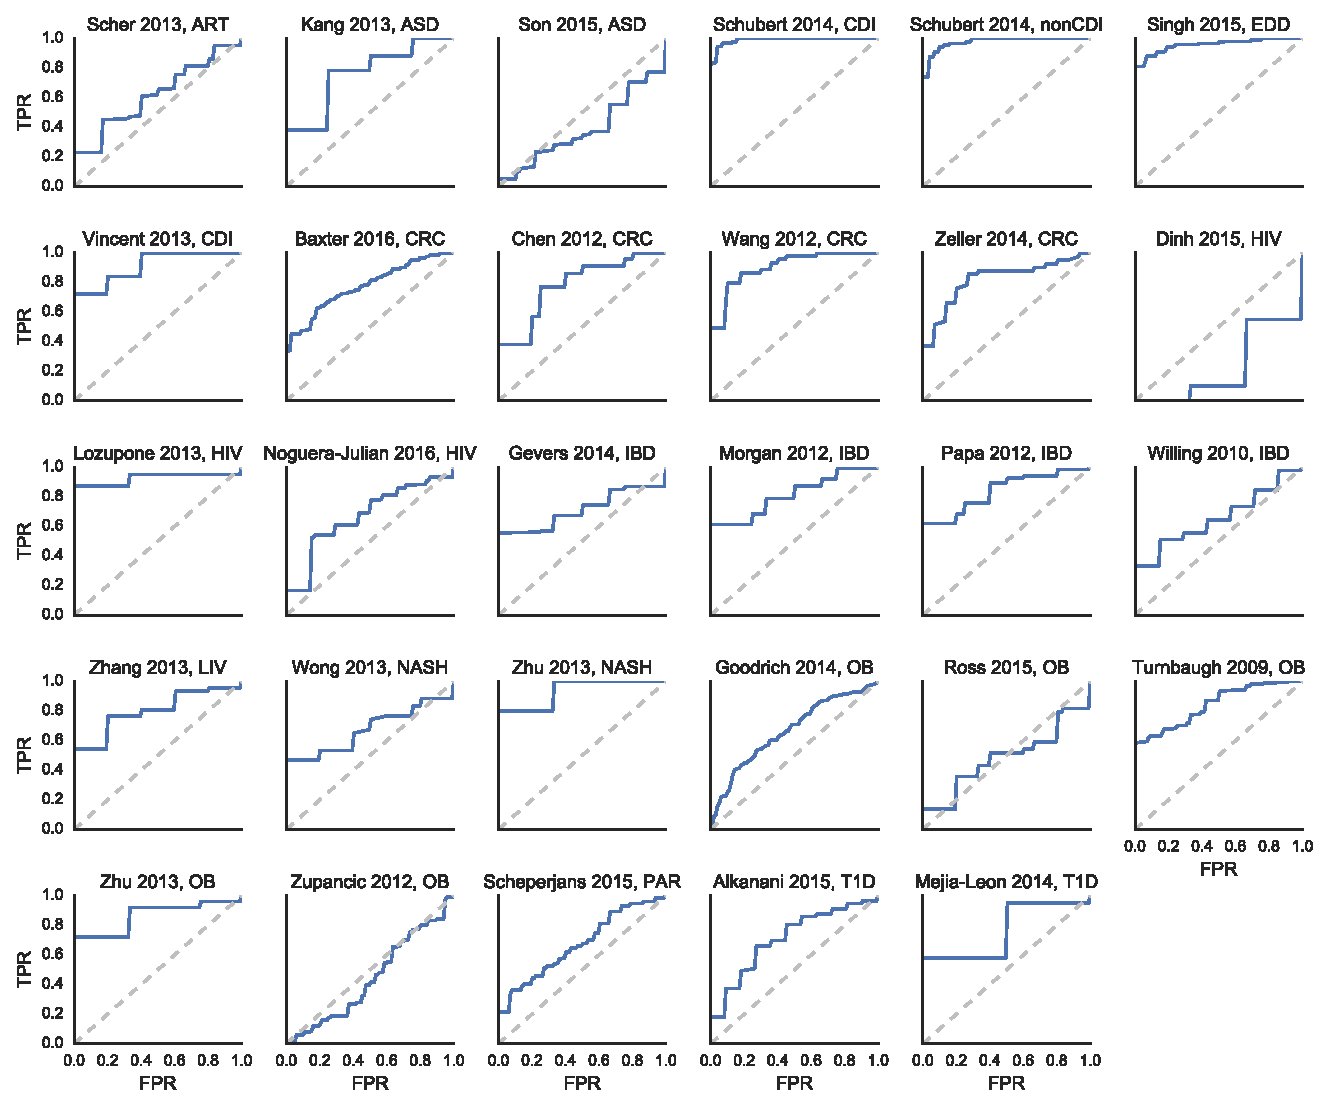
\includegraphics[width=\textwidth]{roc_curves.pdf}}
        \caption{ROC curves for each of the classifiers in Figure 1. Datasets are ordered alphabetically by disease and within disease by first author. FPR = false positive rate, TPR = true positive rate. ART = arthritis, ASD = autism spectrum disorder, CDI = \textit{Clostridium difficile} infection, CRC = colorectal cancer, EDD = enteric diarrheal disease, HIV = human immunodeficient virus, IBD = inflammatory bowel disease, LIV = liver disease, NASH = non-alcoholic steatohepatitis, nonCDI = non-\textit{Clostridium difficile} infection, OB = obesity, PAR = Parkinson's disease, T1D = type I diabetes.
}
        \label{fig:roc_curves}
        \end{center}
\end{figure}

%\newgeometry{textwidth=12in, left=1.5in}
%\newpage \pdfpagewidth=16in \pdfpageheight=18in

\begin{figure}[h]
	\begin{centering}
%	\makebox[\textwidth][c]{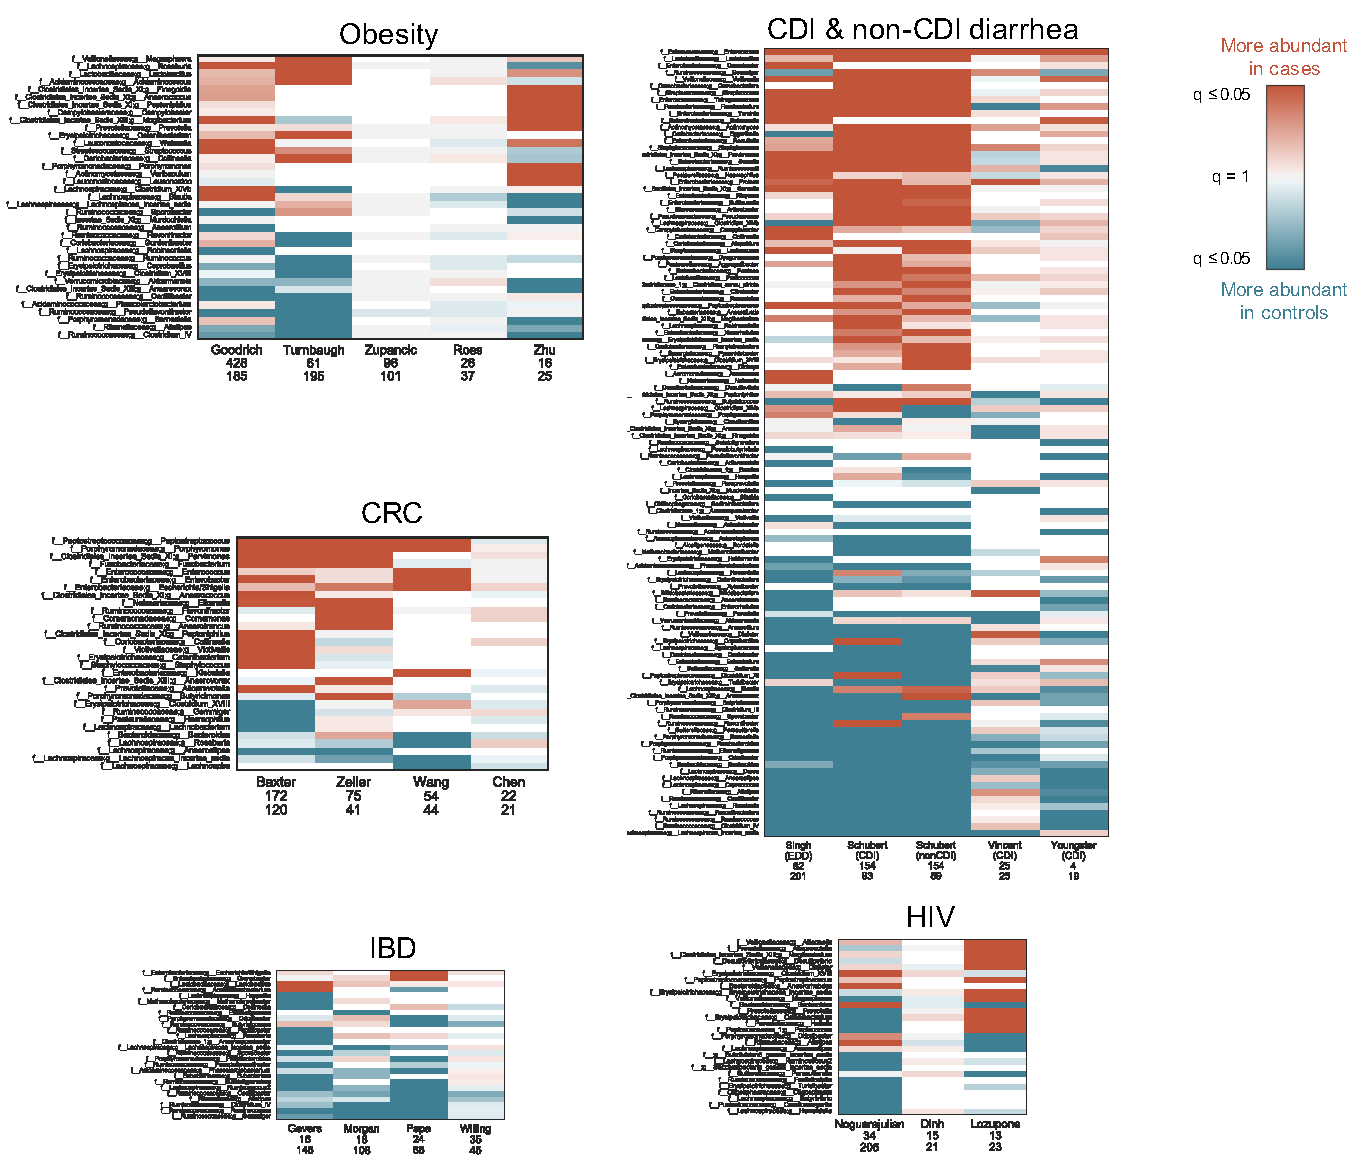
\includegraphics[width=\textwidth]{disease_specific_heatmaps_with_labels.pdf}}%
	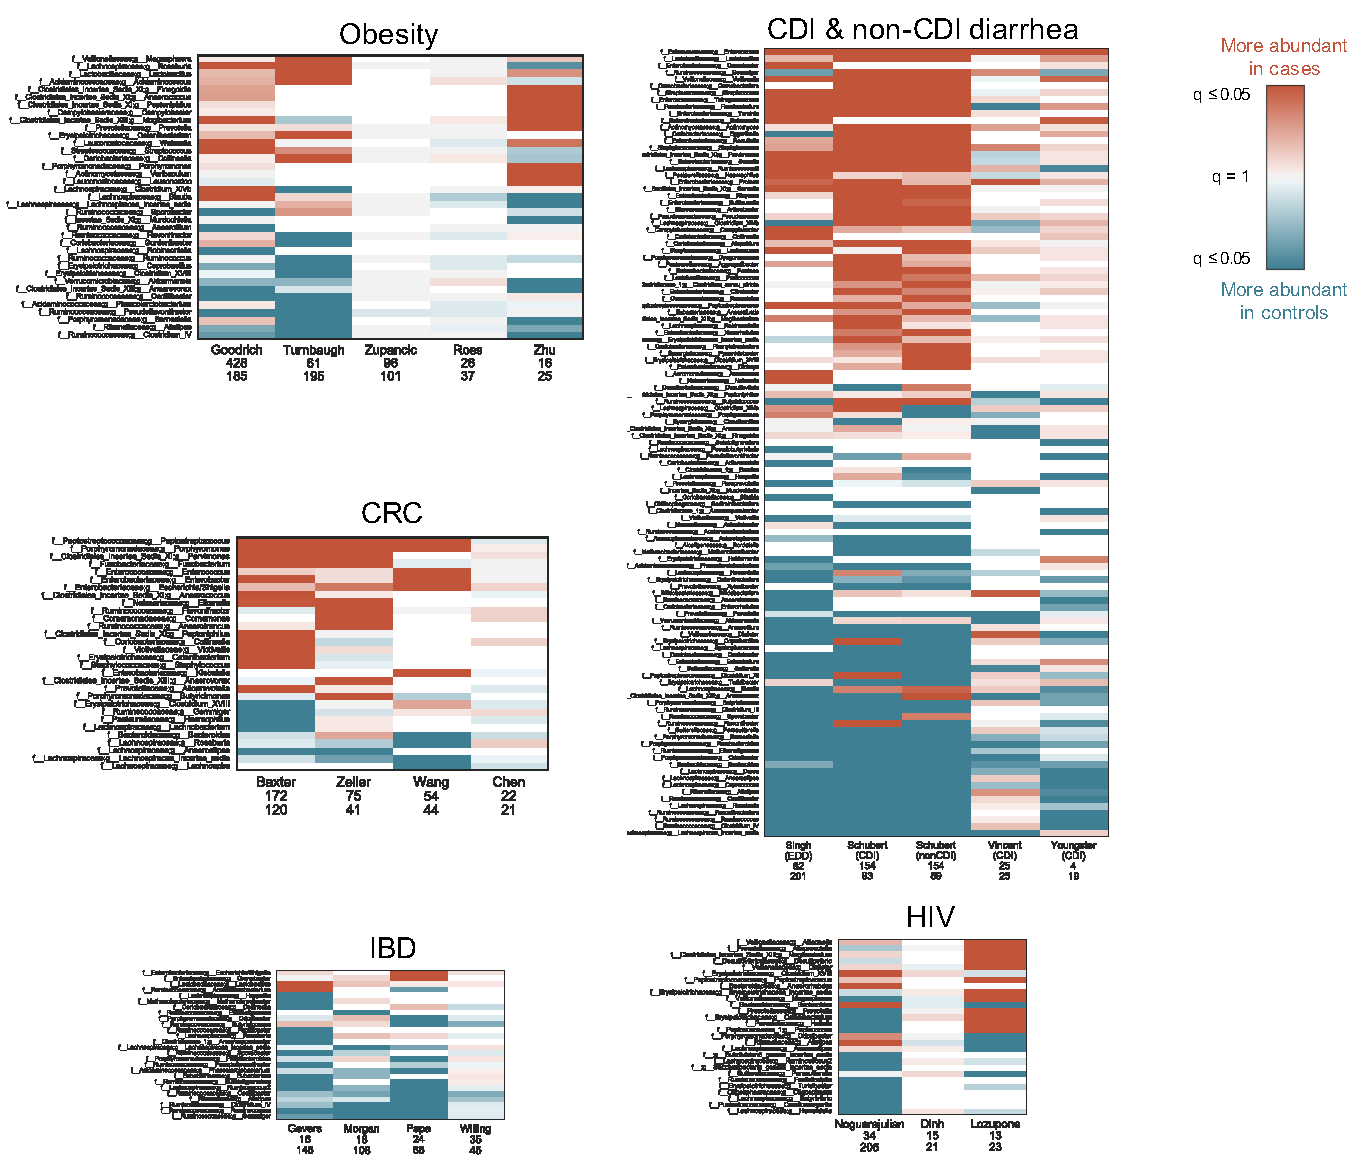
\includegraphics[width=\textwidth]{disease_specific_heatmaps_with_labels.pdf}
	\caption{Same heatmaps as in Figure 2, with rows labeled by family and genus taxonomy. Heatmaps show log10(q-values) for each disease (Kruskal-Wallis (KW) test, Benjamini-Hochberg FDR correction). Rows include all genera which were significant in at least one dataset within each disease, columns are datasets. Q-values are colored by direction of the effect, where red indicates higher mean abundance in disease patients and blue indicates higher mean abundance in controls. Opacity ranges from q = 0.05 to 1, where q values less than 0.05 are the most opaque and q values close to 1 are gray. White indicates that the genus was not present in that dataset. Within each heatmap, rows are ordered from most disease-associated (top) to most health-associated (bottom) (i.e. by the sum across rows of the log10(q-values), signed according to directionality of the effect).
}
	\label{fig:supp_dis_specific}
	\end{centering}
\end{figure}


%\restoregeometry
\FloatBarrier

% Core bugs with genus labels
%\newpage \pdfpagewidth=8.5in \pdfpageheight=27in
\FloatBarrier

\begin{figure}[h]
	\begin{center}
	\makebox[\textwidth][c]{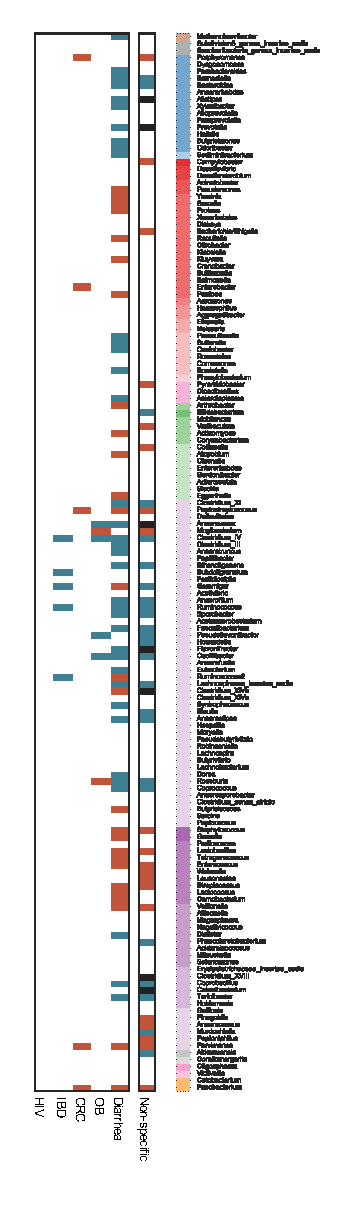
\includegraphics[width=0.37\textwidth]{meta_analysis_with_labels.pdf}}
    \captionsetup{font=footnotesize,labelfont=footnotesize}
	\caption{Panel A from Figure 3, with genus labels. Non-specific and disease-associated genera. Genera are in rows, arranged phylogenetically according to a PhyloT tree built from genus-level NCBI IDs (\url{http://phylot.biobyte.de}). Non-specific genera are associated with health (or disease) in at least two different \textit{diseases} (q $<$ 0.05, Kruskal-Wallis (KW) test, Benjamini-Hochberg FDR correction). Disease-specific genera are significant in the same direction in at least two \textit{studies} of the same disease (q $<$ 0.05, FDR KW test). As in Figure 2, blue indicates higher mean abundance in controls and red indicates higher mean abundance in patients. Black bars indicate mixed genera which were associated with health in two diseases and also associated with disease in two diseases. Disease-specific genera are shown for diseases with at least 3 studies.
}
	\label{fig:supp_meta_heatmap}
	\end{center}
\end{figure}

% Sample size, AUC, n sig, and balance for split cases analyses
\FloatBarrier
%\newpage \pdfpagewidth=8.5in \pdfpageheight=10in

\begin{figure}[h]
	\begin{center}
	\makebox[\textwidth][c]{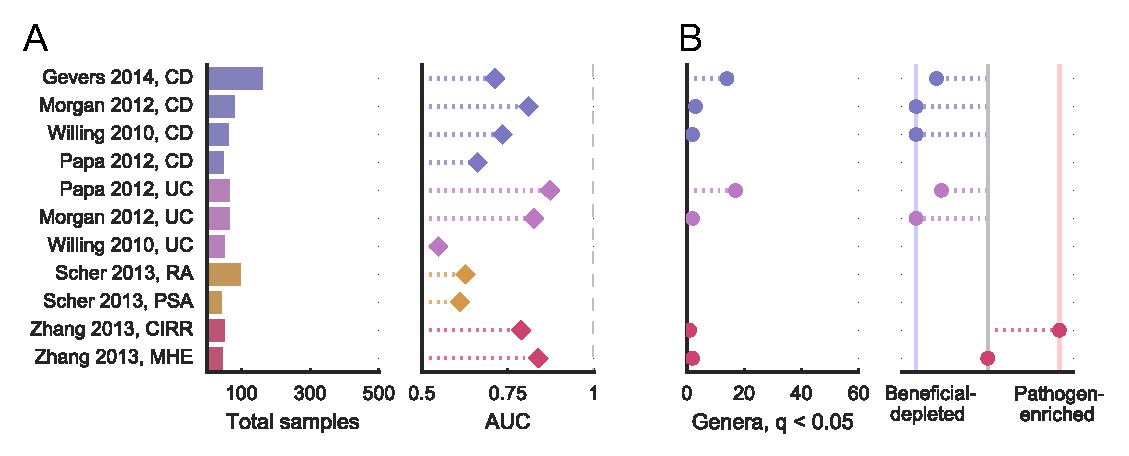
\includegraphics[width=\textwidth]{samplesize_auc_nsig_balance_split_cases.pdf}}%
	\caption{Same analysis as in Figure 1 for stratified patient groups. (A) Left: Total sample size for each comparison. Right: Area under the ROC curve (AUC) for genus-level random forest classifiers. (B) Left: Number of genera with q $<$ 0.05 (Kruskal-Wallis (KW) test, Benjamini-Hochberg FDR correction) for each type of patient group comparison. Right: Direction of microbiome shift,i.e. the percent of total associated genera which were enriched in diseased patients. In comparisons on the leftmost blue line, 100\% of associated (q $<$ 0.05, FDR KW test) genera are health-associated (i.e. depleted in patients relative to controls). In comparisons on the rightmost red line, 100\% of associated (q $<$ 0.05, FDR KW test) genera are disease-associated (i.e. enriched in patients relative to controls).
}
	\label{fig:split_cases_fig1}
	\end{center}
\end{figure}

% CD and UC qvalues heatmaps
\newpage
\begin{figure}[h]
	\begin{center}
	\makebox[\textwidth][c]{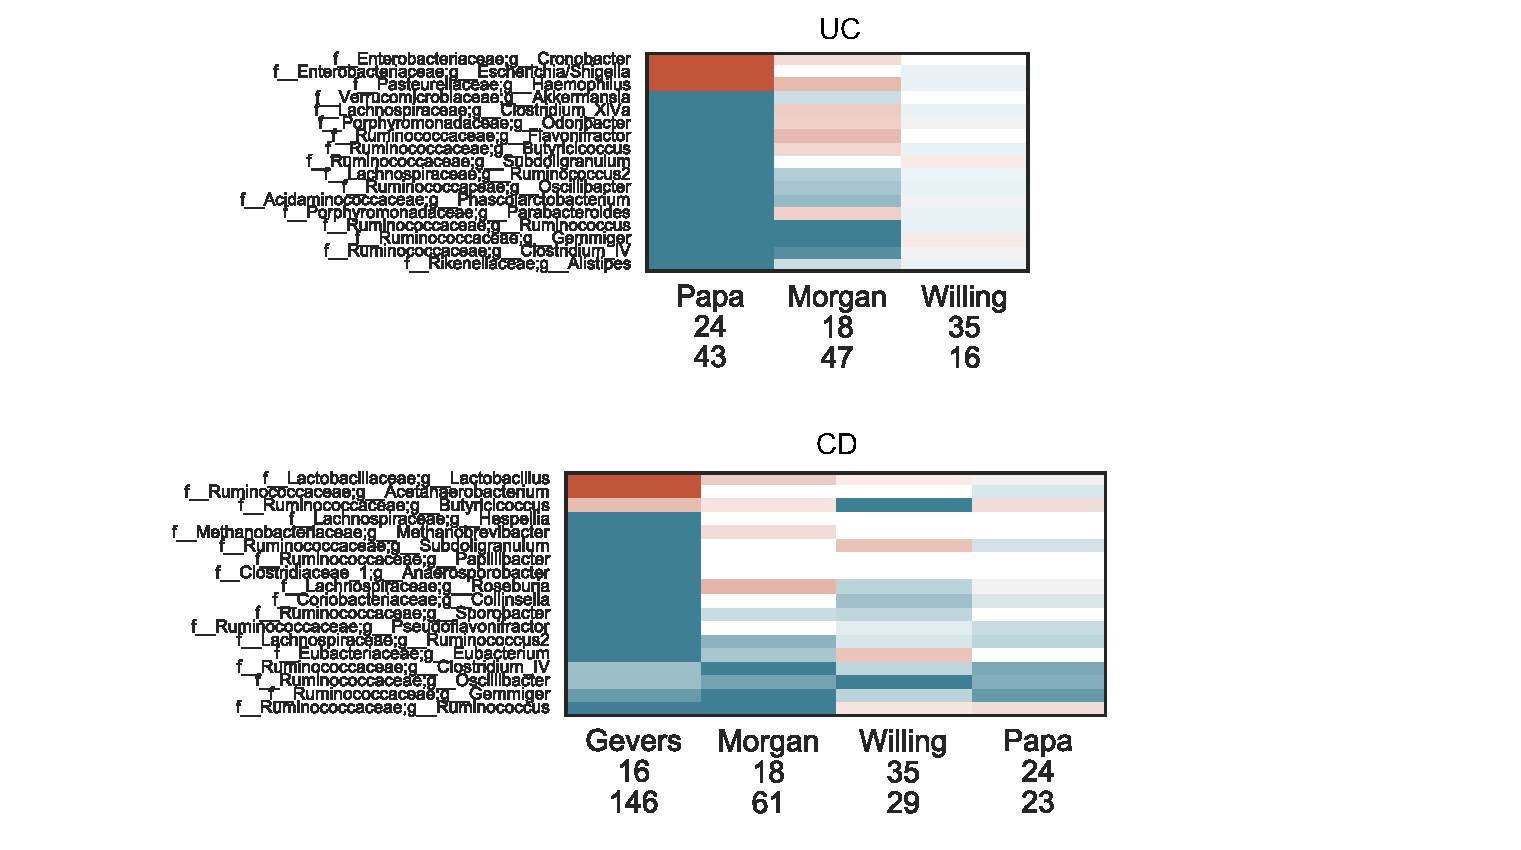
\includegraphics[width=1.1\textwidth]{disease_specific_heatmaps_with_labels_split_cases.pdf}}%
	\caption{Same results as presented in Figure 2 for ulcerative colitis (UC) and Crohn's disease (CD) IBD patients separately. Heatmaps show log10(q-values) for each comparison, with studies in columns and genera in rows (Kruskal-Wallis (KW) test, Benjamini-Hochberg FDR correction). Q-values are colored by direction of the effect, where red indicates higher mean abundance in disease patients and blue indicates higher mean abundance in controls. Opacity ranges from q = 0.05 to 1, where q values less than 0.05 are the most opaque and q values close to 1 are gray. White indicates that the genus was not present in that dataset. Within each heatmap, rows are ordered from most disease-associated (top) to most health-associated (bottom) (i.e. by the sum across rows of the log10(q-values), signed according to directionality of the effect).
}
	\label{fig:split_cases_heatmaps}
	\end{center}
\end{figure}

% Shannon alpha diversity
\newpage
\begin{figure}[h]
	\begin{center}
	\makebox[\textwidth][c]{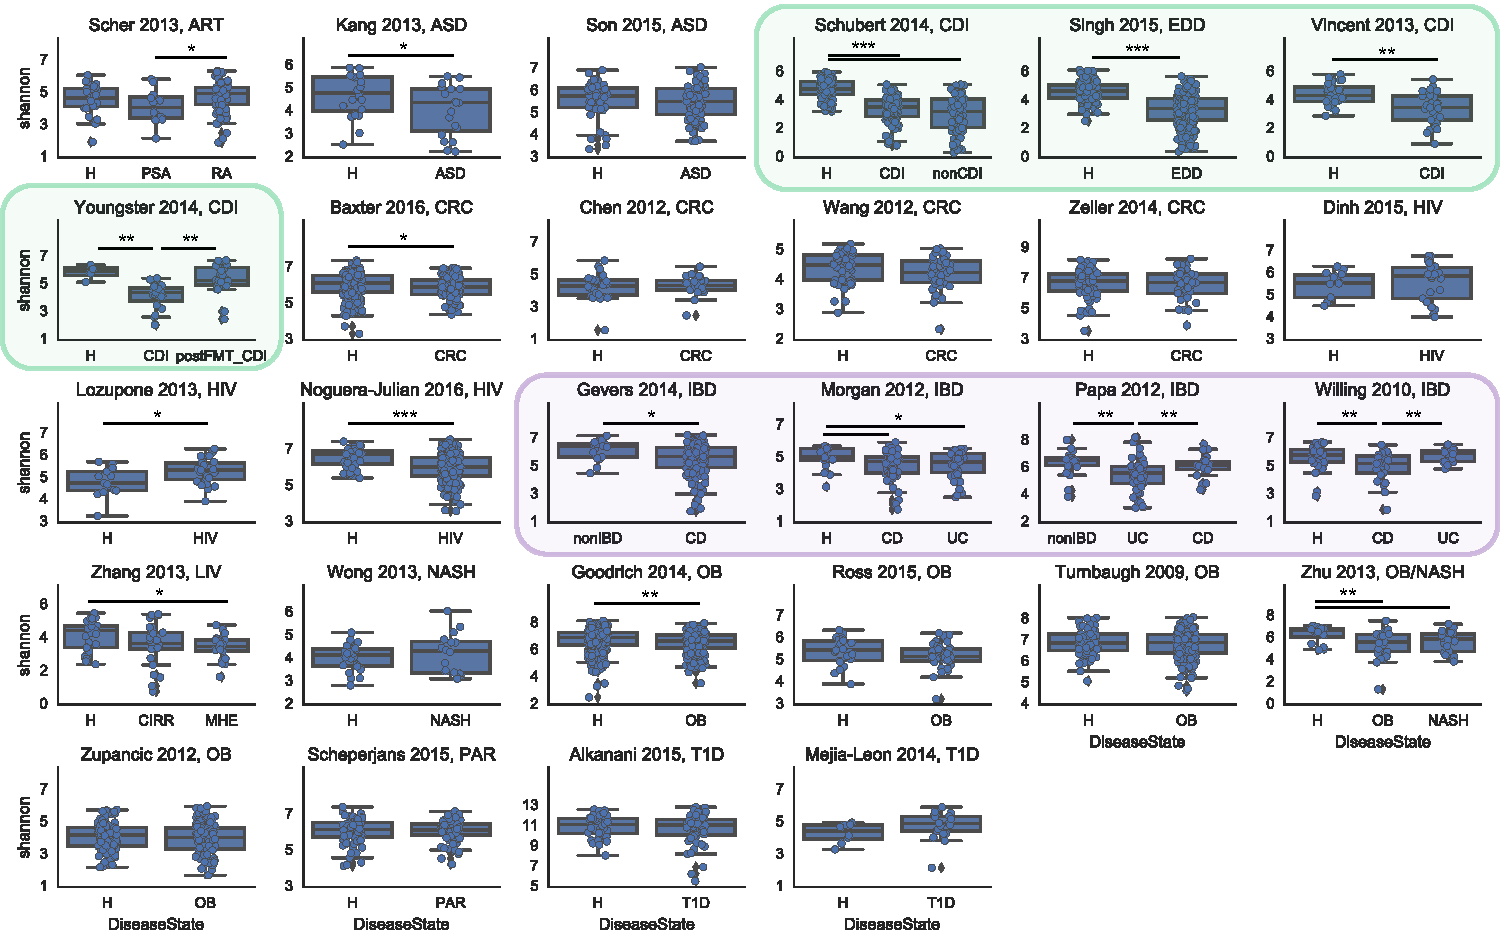
\includegraphics[width=\textwidth]{alpha_diversity_shannon.pdf}}
    \captionsetup{font=footnotesize,labelfont=footnotesize}
	\caption{Reduction in alpha diversity is not a reliable indicator of ``dysbiosis.'' Shannon alpha diversity index across all patient groups in all studies, calculated on OTUs (i.e. not collapsed to genus level, and including unannotated OTUs). Diarrheal patients consistently have lower alpha diversity than non-diarrheal controls (green box). Crohn's disease (CD) patients also show a slight reduction of alpha diversity relative to controls in three out of four IBD studies and ulcerative colitis (UC) patients in two studies (purple box). Obese patients have inconsistent and small reductions in alpha diversity, consistent with a previous meta-analysis \cite{Sze07092016}. $\ast: 0.01 < p < 0.05, \ast\ast: 10^{-4} < p < 0.01, \ast\ast\ast: p < 10^{-4}$. P values are calculated from a two-sided T-test (using \texttt{scipy.stats.ttest\_ind}) and are not corrected for multiple tests. Note that the datasets with multiple case groups (Zhu et al. (OB/NASH, 2013) and Schubert et al. (CDI/non-CDI, 2014)) are presented only once in this plot. ART = arthritis, ASD = austism spectrum disorder, CD = Crohn's disease, CDI = \textit{Clostridium difficile} infection, CIRR = liver cirrhosis, CRC = colorectal cancer, EDD = enteric diarrheal disease, H = healthy, HIV = human immunodeficiency virus, LIV = liver diseases,  MHE =  minimal hepatic encephalopathy, NASH = non-alcoholic steatohepatitis, OB = obesity, PAR = Parkinson's disease, PSA = psoriatic arthritis, RA = rheumatoid arthritis, T1D = type I diabetes, UC = ulcerative colitis. nonCDI controls are patients with diarrhea who tested negative for \textit{C. difficile} infection. nonIBD controls are patients  with gastrointestinal symptoms but no intestinal inflammation.
}
	\label{fig:fig_alpha}
	\end{center}
\end{figure}

% Chao1 alpha diversity
\newpage
\begin{figure}[h]
	\begin{center}
	\makebox[\textwidth][c]{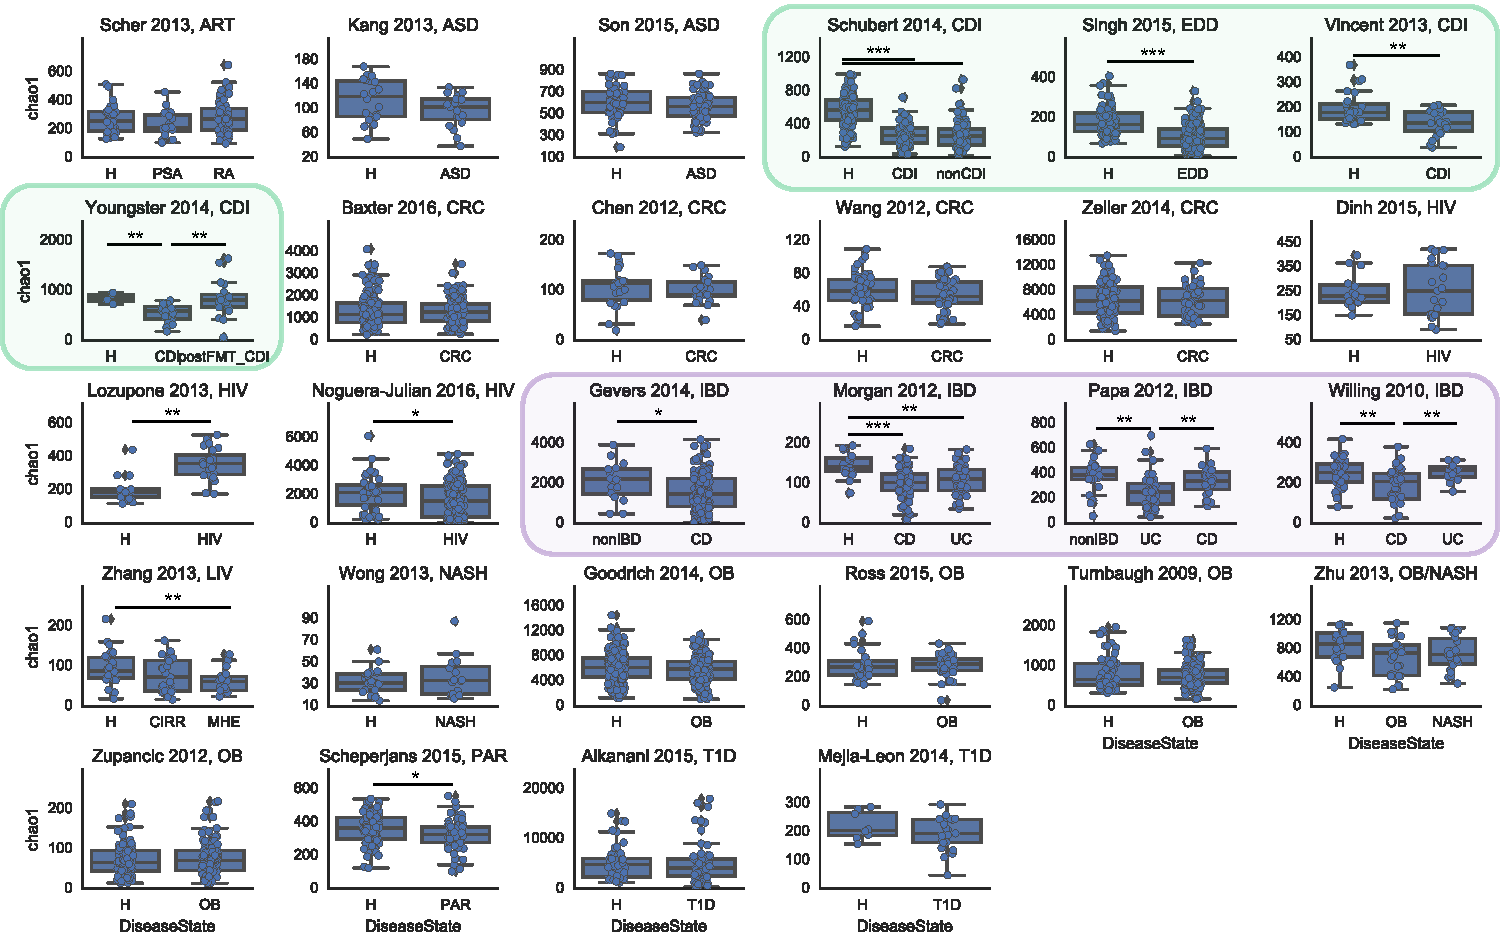
\includegraphics[width=1\textwidth]{alpha_diversity_chao1.pdf}}
    \captionsetup{font=footnotesize,labelfont=footnotesize}
	\caption{Chao1 alpha diversity across all patient groups in all studies, calculated on OTUs (i.e. not collapsed to genus level, and including unannotated OTUs). $\ast: 0.01 < p < 0.05, \ast\ast: 10^{-4} < p < 0.01, \ast\ast\ast: p < 10^{-4}$. P values are calculated from a two-sided T-test (using \texttt{scipy.stats.ttest\_ind}) and are not corrected for multiple tests. Note that the datasets with multiple case groups (Zhu et al. (OB/NASH, 2013) and Schubert et al. (CDI/non-CDI, 2014)) are presented only once in this plot. ART = arthritis, ASD = austism spectrum disorder, CD = Crohn's disease, CDI = \textit{Clostridium difficile} infection, CIRR = liver cirrhosis, CRC = colorectal cancer, EDD = enteric diarrheal disease, H = healthy, HIV = human immunodeficiency virus, LIV = liver diseases,  MHE =  minimal hepatic encephalopathy, NASH = non-alcoholic steatohepatitis, OB = obesity, PAR = Parkinson's disease, PSA = psoriatic arthritis, RA = rheumatoid arthritis, T1D = type I diabetes, UC = ulcerative colitis. nonCDI controls are patients with diarrhea who tested negative for \textit{C. difficile} infection. nonIBD controls are patients  with gastrointestinal symptoms but no intestinal inflammation.
}
	\label{fig:fig_alpha_chao1}
	\end{center}
\end{figure}

% Simpson alpha diversity
\newpage
\begin{figure}[h]
	\begin{center}
	\makebox[\textwidth][c]{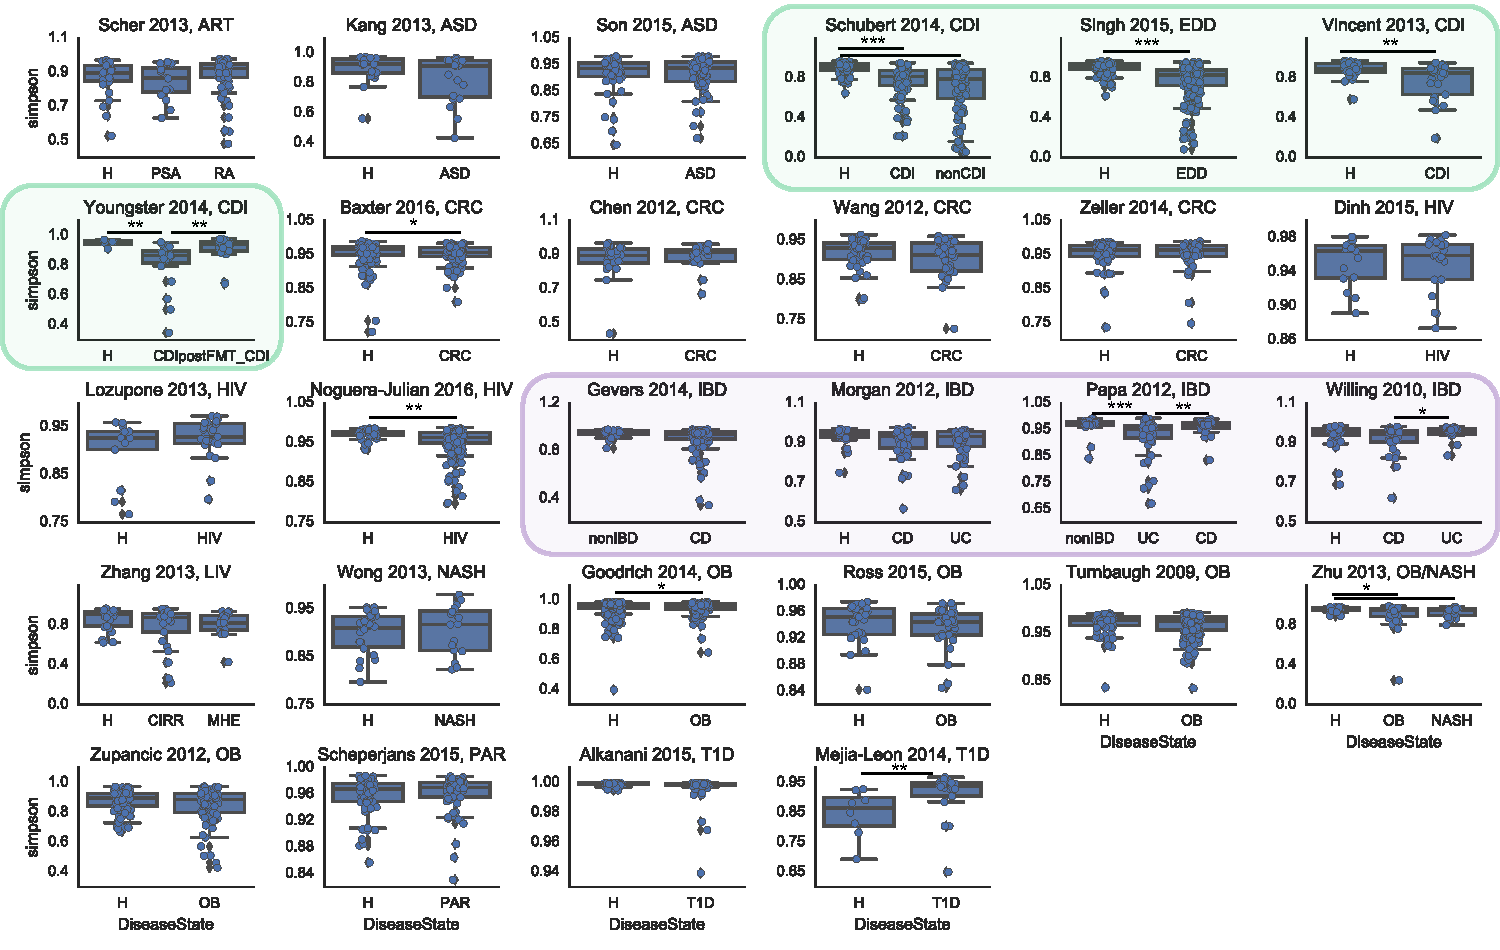
\includegraphics[width=\textwidth]{alpha_diversity_simpson.pdf}}
    \captionsetup{font=footnotesize,labelfont=footnotesize}
	\caption{Simpson alpha diversity across all patient groups in all studies, calculated on OTUs (i.e. not collapsed to genus level, and including unannotated OTUs). $\ast: 0.01 < p < 0.05, \ast\ast: 10^{-4} < p < 0.01, \ast\ast\ast: p < 10^{-4}$. P values are calculated from a two-sided T-test (using \texttt{scipy.stats.ttest\_ind}) and are not corrected for multiple tests. Note that the datasets with multiple case groups (Zhu et al. (OB/NASH, 2013) and Schubert et al. (CDI/non-CDI, 2014)) are presented only once in this plot. ART = arthritis, ASD = austism spectrum disorder, CD = Crohn's disease, CDI = \textit{Clostridium difficile} infection, CIRR = liver cirrhosis, CRC = colorectal cancer, EDD = enteric diarrheal disease, H = healthy, HIV = human immunodeficiency virus, LIV = liver diseases,  MHE =  minimal hepatic encephalopathy, NASH = non-alcoholic steatohepatitis, OB = obesity, PAR = Parkinson's disease, PSA = psoriatic arthritis, RA = rheumatoid arthritis, T1D = type I diabetes, UC = ulcerative colitis. nonCDI controls are patients with diarrhea who tested negative for \textit{C. difficile} infection. nonIBD controls are patients  with gastrointestinal symptoms but no intestinal inflammation.
}
	\label{fig:fig_alpha_simpson}
	\end{center}
\end{figure}

% Healthy vs. disease classifier
\newpage
\begin{figure}[h]
	\begin{center}
	\makebox[\textwidth][c]{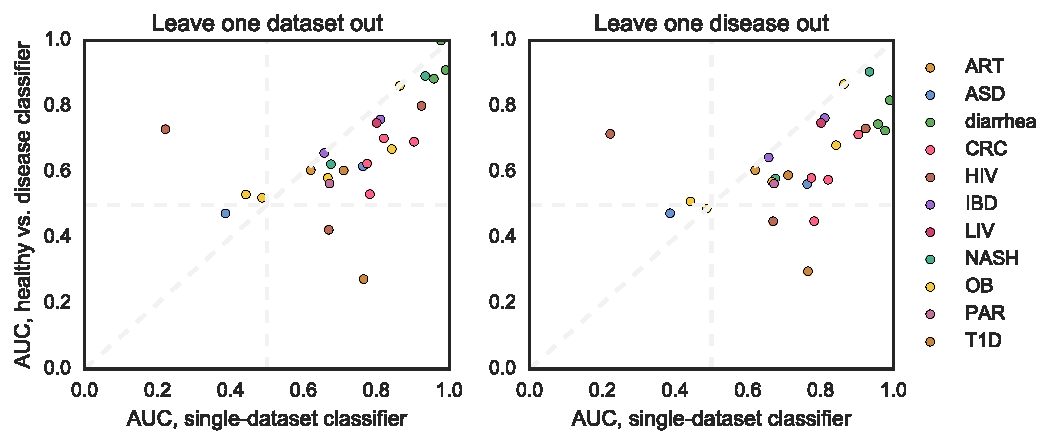
\includegraphics[width=1\textwidth]{healthy_vs_disease_classifier.pdf}}%
	\caption{\textit{Both x-axes}: the area under the ROC curve (AUC) from each dataset's single classifier. Left: leave-one-dataset-out classifier. \textit{y-axis}: the AUC of a classifier trained on all other datasets to distinguish healthy from unhealthy patients, tested on the left out dataset. Right: leave-one-disease-out classifier. \textit{y-axis}: AUC from a classifier trained to distinguish healthy from unhealthy patients on all datasets except those of the tested disease. AUCs for each dataset were built from the classification probabilities on each test sample.
}
	\label{fig:overall_classifier}
	\end{center}
\end{figure}

% Different ways to define core response
\FloatBarrier
%\newpage \pdfpagewidth=8.5in \pdfpageheight=15in

\begin{figure}[h]
	\begin{center}
	\makebox[\textwidth][c]{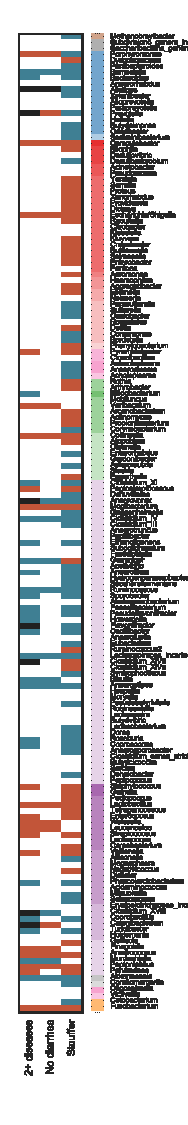
\includegraphics[width=0.22\textwidth]{different_core_defns.pdf}}
    \captionsetup{font=footnotesize,labelfont=footnotesize}
	\caption{The majority of non-specific microbes are robust to the exclusion of diarrhea datasets from consideration. The right-most bar shows order-level phylogeny, colored as in Figure 3A of the main paper. The left bar of the heatmap shows the original non-specific microbes, including all datasets. The middle bar shows the re-defined non-specific responders after excluding all diarrhea datasets. The right bar of the heatmap shows the non-specific microbes defined using Stouffer’s method, combining one-tailed q-values across datasets and weighting by the square root of sample size (Stouffer combined q $<$ 0.05).
}
	\label{fig:core_defns}
	\end{center}
\end{figure}


% Significance of shared response
\FloatBarrier
%\newpage \pdfpagewidth=8.5in \pdfpageheight=11in

\begin{figure}[h]
	\begin{center}
	\makebox[\textwidth][c]{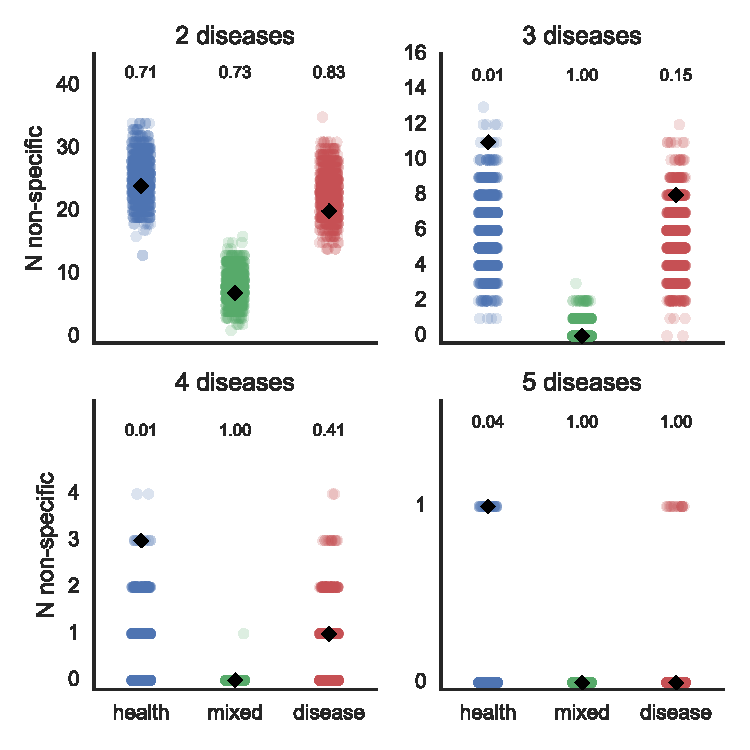
\includegraphics[width=\textwidth]{core_significance.pdf}}%
	\caption{Empirical null distribution of the number of non-specific responders (colored points, x-axis indicates directionality of response), overlayed with the actual observed number of non-specific responders (black diamonds) for different defining heuristics (axis titles, i.e. ``3 diseases`` means that a genus needed to be significant (q $<$ 0.05, Kruskal-Wallis (KW) test, Benjamini-Hochberg FDR correction) in three diseases in the same direction to be considered a non-specific responder). Empirical one-tailed p-values are printed above each distribution.
}
	\label{fig:core_sig}
	\end{center}
\end{figure}

% RF param search - gini criteria
\newpage
\begin{landscape}
\begin{figure}[h]
	\begin{center}
	\makebox[\textwidth][c]{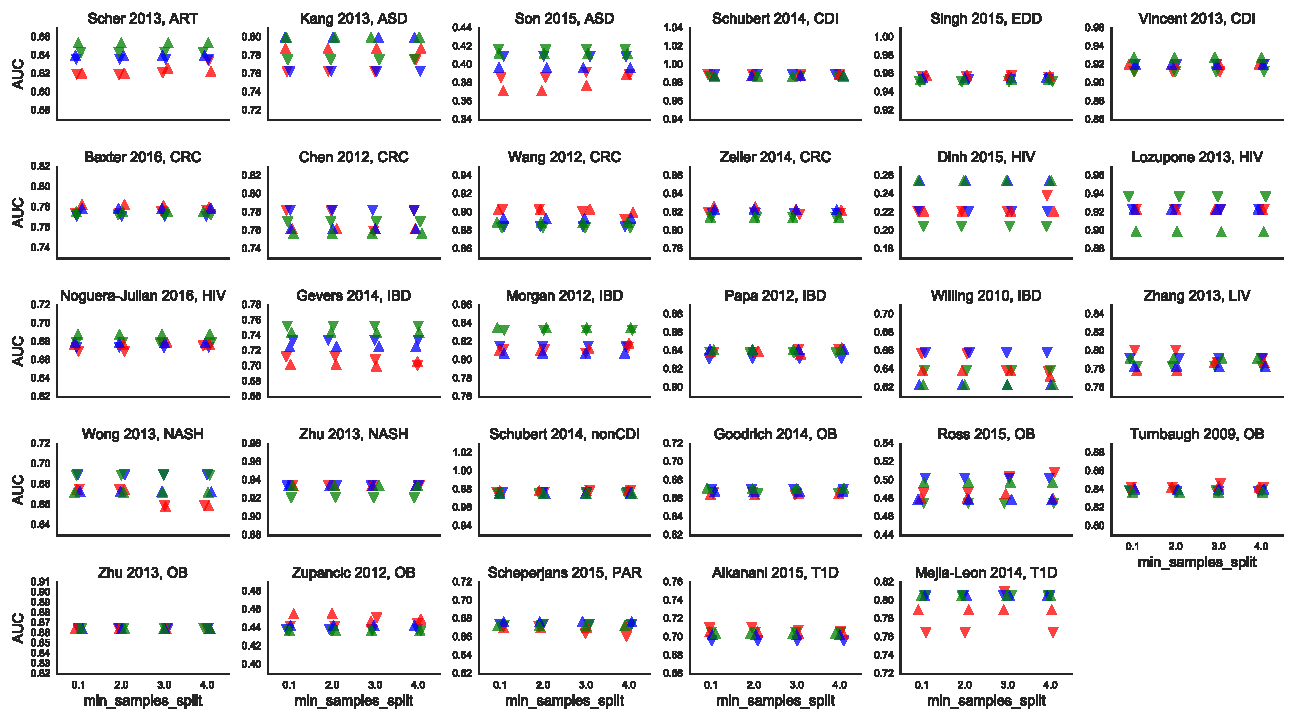
\includegraphics[width=1.4\textwidth]{rf_params_gini.pdf}}%
	\caption{Varying Random Forest parameters does not significantly affect area under the ROC curve in classifying cases from controls (Gini criteria). Random Forest classifiers built by using the Gini impurity (``gini'') split criteria (``scikit-learn RandomForestClassifier''). Upward-pointing triangles are classifiers built with 10000 estimators; downward-pointing triangles are built with 1000 estimators. Colors indicate the value of \texttt{min\_samples\_leaf} (the minimum number of samples required to be at a leaf node): red = 1, blue = 2, green = 3. X-axes are the value of \texttt{min\_samples\_split} (the minimum number of samples required to split an internal node) \cite{scikit-learn}. All Random Forests were built using the random state seed $12345$.
}
	\label{fig:rf_params_gini}
	\end{center}
\end{figure}

% RF param search - entropy criteria
\newpage
\begin{figure}[h]
	\begin{center}
	\makebox[\textwidth][c]{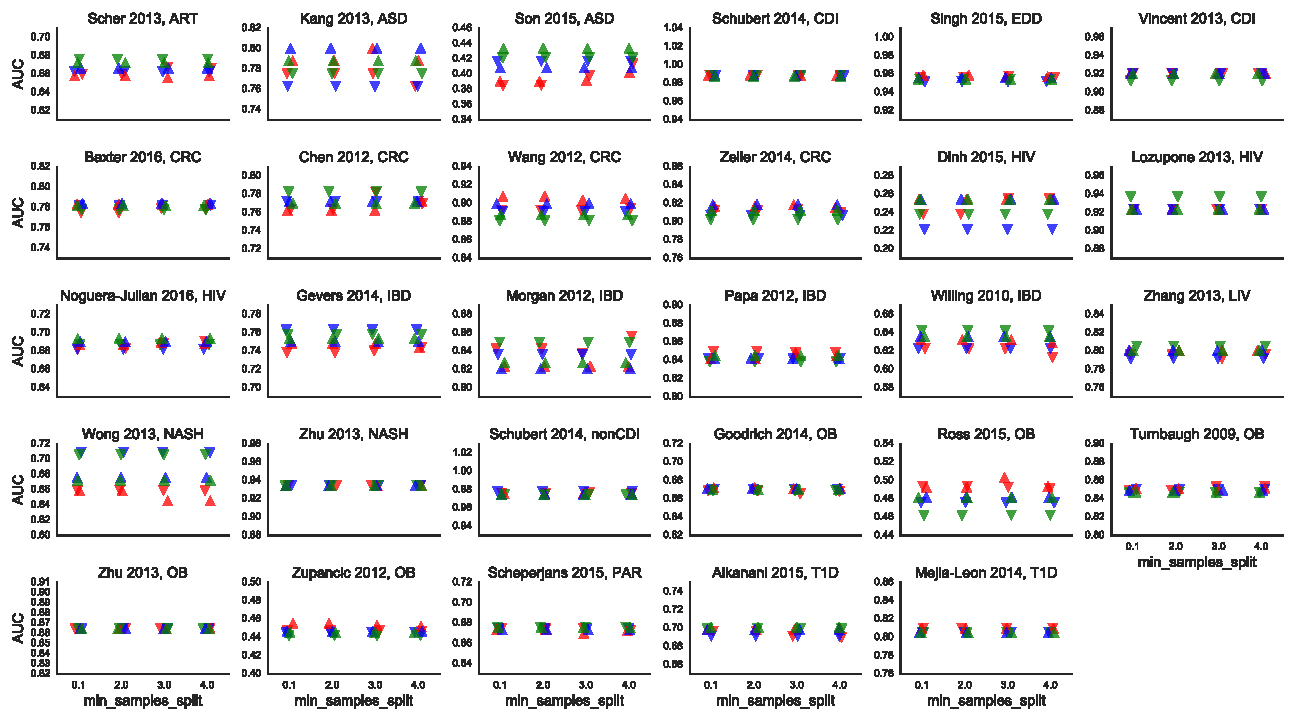
\includegraphics[width=1.4\textwidth]{rf_params_entropy.pdf}}%
	\caption{Varying Random Forest parameters does not significantly affect area under the ROC curve in classifying cases from controls (entropy criteria). Random Forest classifiers built by using the entropy (``entropy'') split criteria (``scikit-learn RandomForestClassifier''). Upward-pointing triangles are classifiers built with 10000 estimators; downward-pointing triangles are built with 1000 estimators. Colors indicate the value of \texttt{min\_samples\_leaf} (the minimum number of samples required to be at a leaf node): red = 1, blue = 2, green = 3. X-axes are the value of \texttt{min\_samples\_split} (the minimum number of samples required to split an internal node) \cite{scikit-learn}. All Random Forests were built using the random state seed $12345$.
}
	\label{fig:rf_params_entropy}
	\end{center}
\end{figure}
\end{landscape}

% Heatmap with results for all datasets (all sig genera) - qvalues
\FloatBarrier
%\newgeometry{textwidth=18in, left=1.5in}
%\newpage \pdfpagewidth=28in \pdfpageheight=28in

\begin{figure}[h]
	\begin{center}
	\makebox[\textwidth][c]{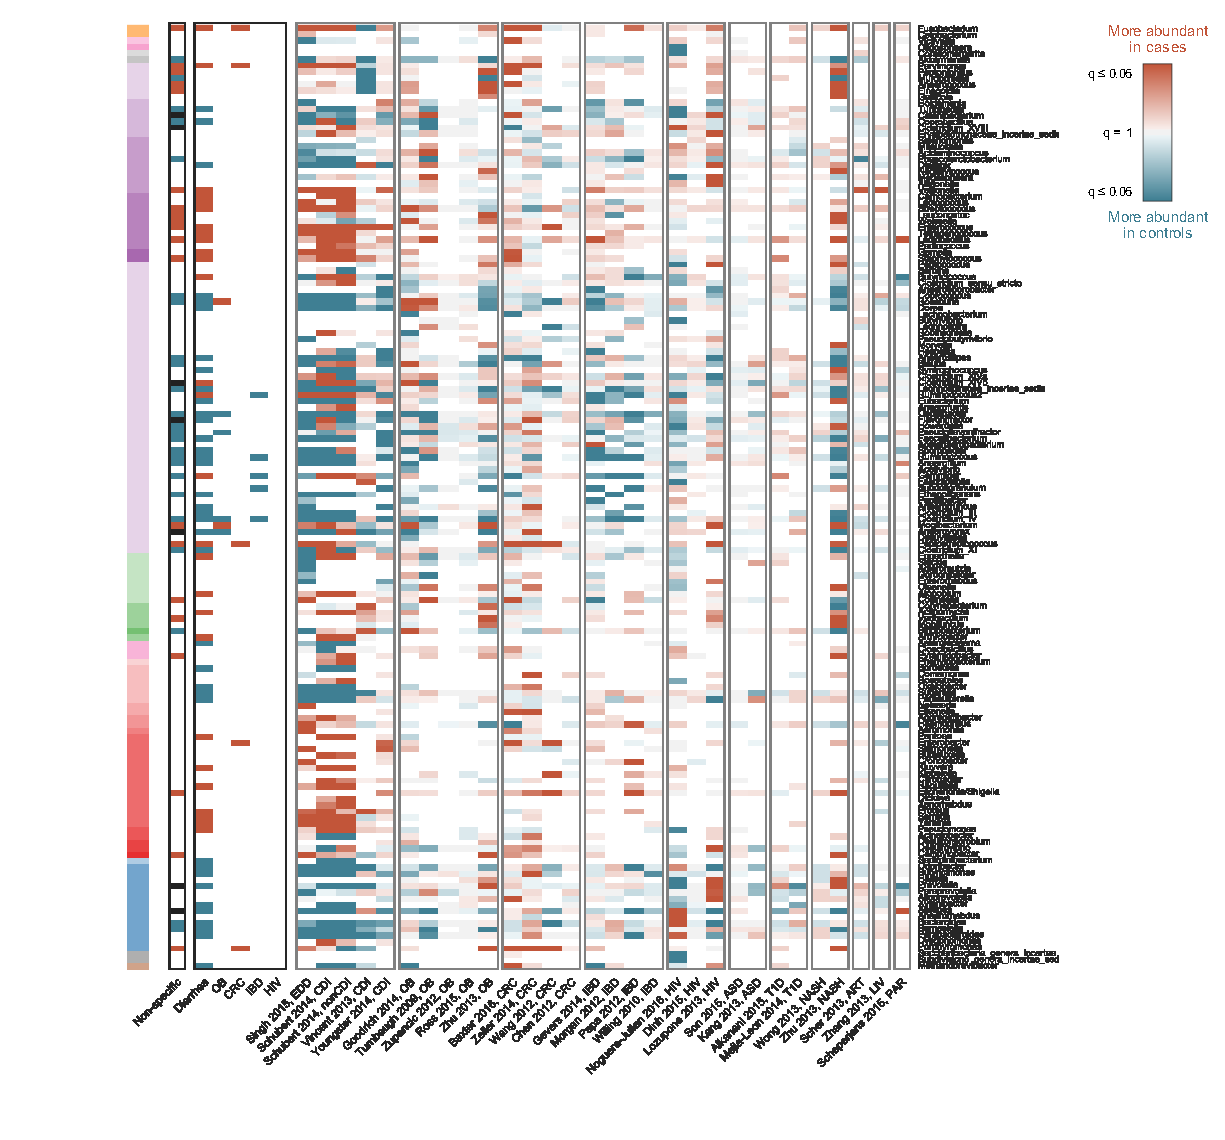
\includegraphics[width=1.2\textwidth]{overall_heatmap_log10qvalues.pdf}}
	%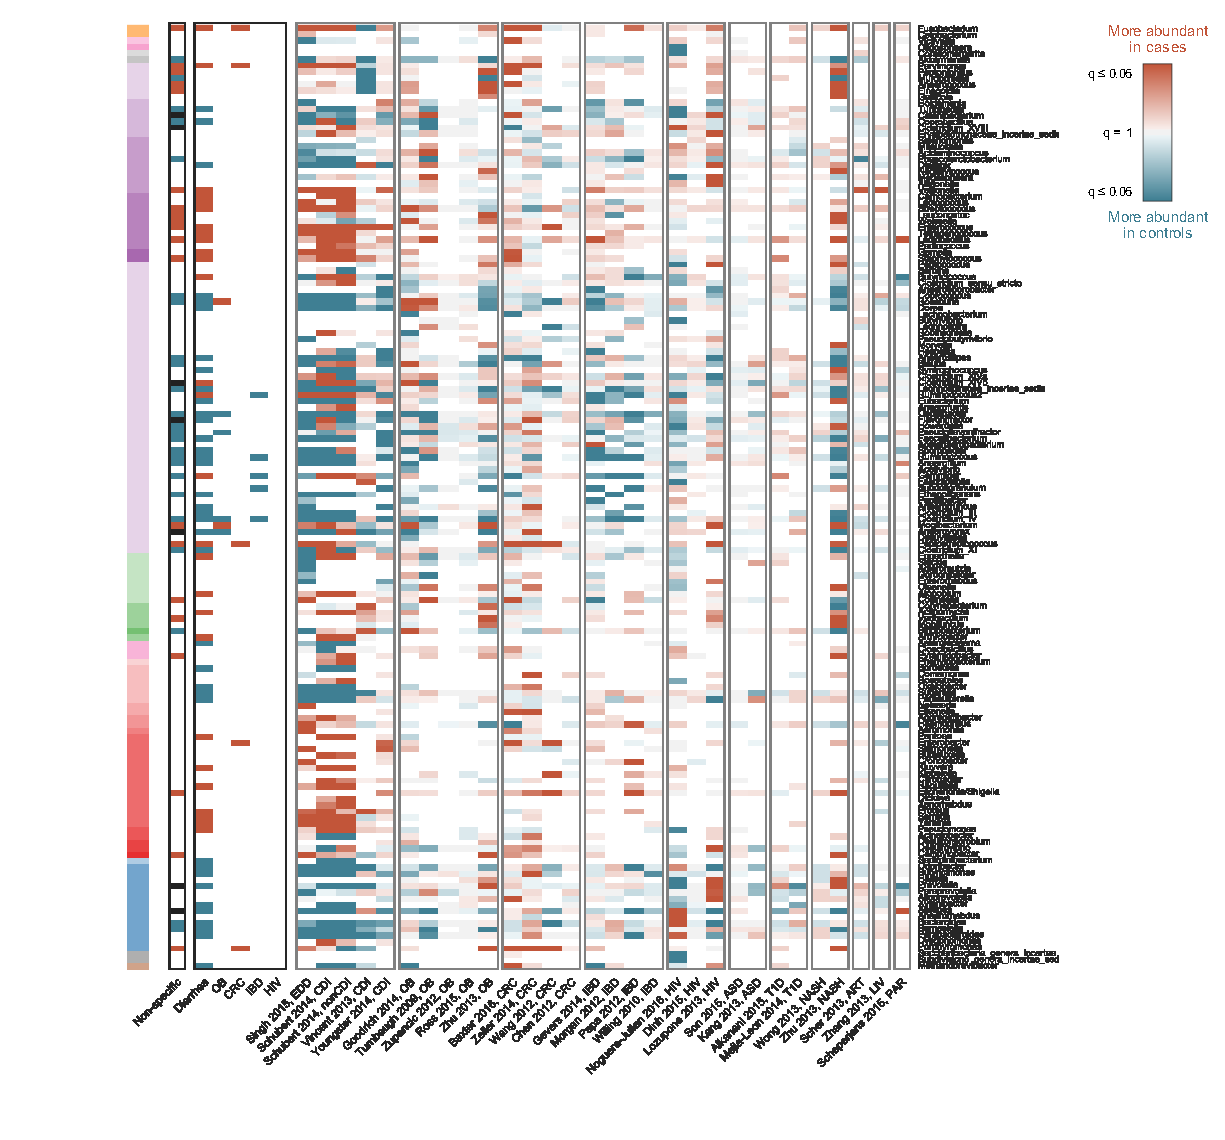
\includegraphics[width=1.2\textwidth]{overall_heatmap_log10qvalues.pdf}
    \captionsetup{font=footnotesize,labelfont=footnotesize}
	\caption{Heatmap of log10(q values) for all genera which were significant (q $<$ 0.05, Kruskal-Wallis (KW) test, Benjamini-Hochberg FDR correction) in at least one dataset, across all studies. Rows are genera, ordered phylogenetically (as in Figure 3A). Columns are datasets, grouped by disease and ordered according to total sample size (decreasing from left to right). The first and second heatmap panels from the left are the same as in Figure 3A. Q-values are colored according to directionality of the effect, where red indicates higher mean abundance in patients relative to controls and blue indicates higher mean abundance in controls. Opacity indicates significance and ranges from 0.05 to 1, where q-values less than 0.05 are the darkest colors and q-values close to 1 are gray. White indicates that the genus was not present in that dataset. ART = arthritis, ASD = autism spectrum disorder, CDI = \textit{Clostridium difficile} infection, CRC = colorectal cancer, EDD = enteric diarrheal disease, HIV = human immunodeficient virus, IBD = inflammatory bowel disease, LIV = liver disease, NASH = non-alcoholic steatohepatitis, nonCDI = non-\textit{Clostridium difficile} infection, OB = obesity, PAR = Parkinson's disease, T1D = type I diabetes.
}
	\label{fig:overall_heatmap_qvalues}
	\end{center}
\end{figure}

% Heatmap with results for all datasets (all sig genera) - effect size
\newpage
\begin{figure}[h]
	\begin{center}
	\makebox[\textwidth][c]{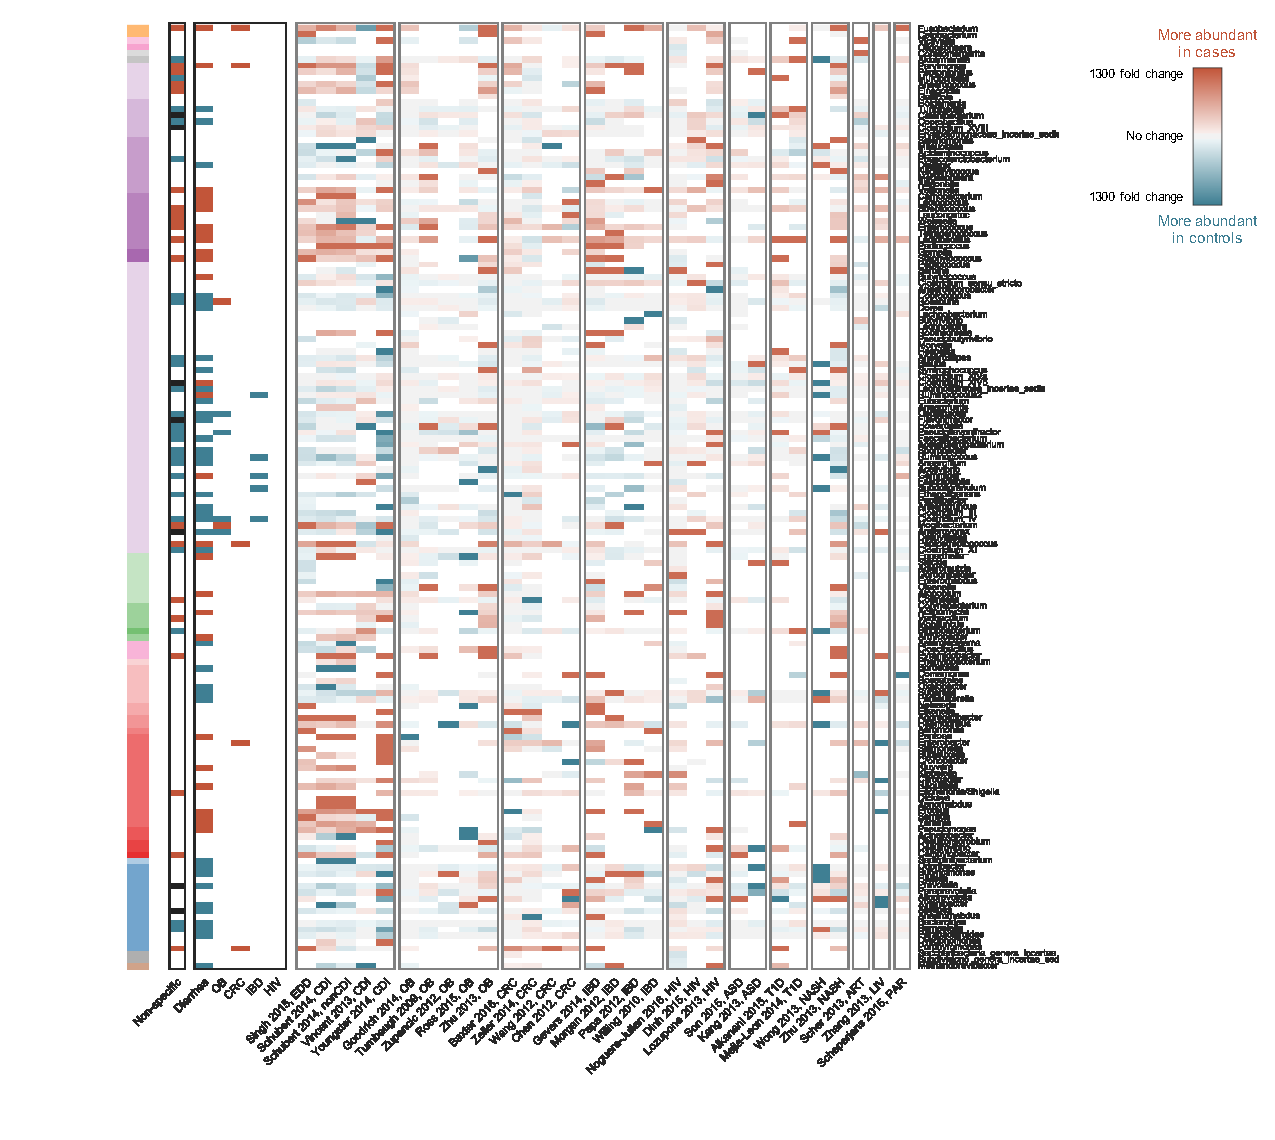
\includegraphics[width=1.2\textwidth]{overall_heatmap_log2change.pdf}}
	%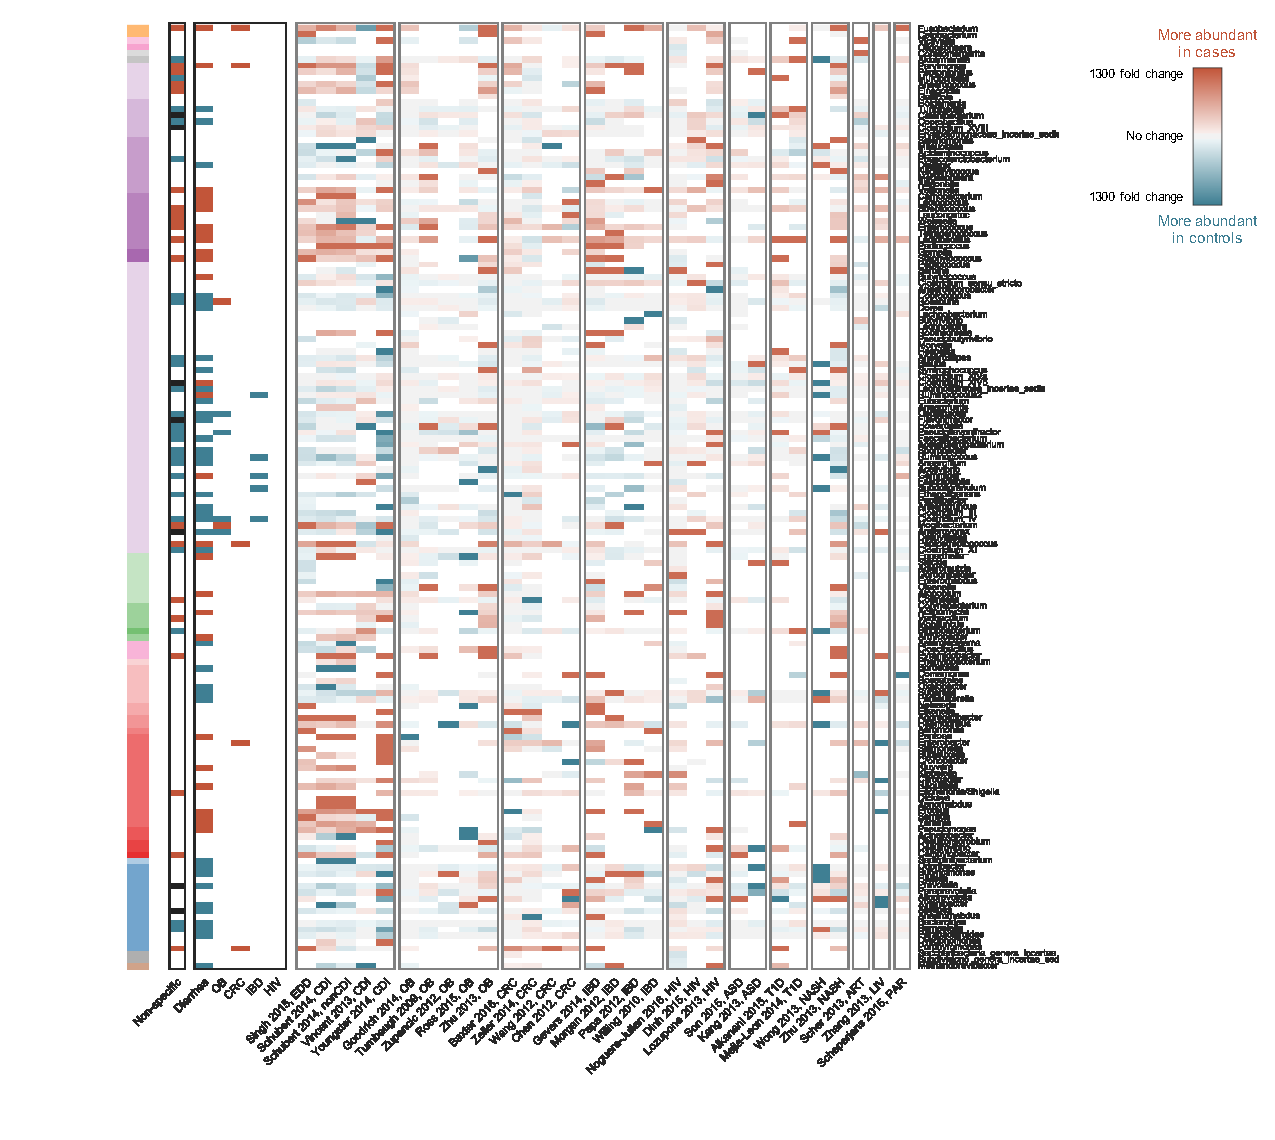
\includegraphics[width=24in]{overall_heatmap_log2change.pdf}
    \captionsetup{font=footnotesize,labelfont=footnotesize}
	\caption{Heatmap of log-fold change between cases and controls (i.e. $log_2(\frac{\text{mean abundance in cases}}{\text{mean abundance in controls}}$) for all genera which were significant (q $<$ 0.05) in at least one dataset, across all studies. Rows are genera, ordered phylogenetically (as in Figure 3A). Columns are datasets, grouped by disease and ordered according to total sample size (decreasing from left to right). The first and second heatmap panels from the left are the same as in Figure 3A. Values are colored according to directionality of the effect, where red indicates higher mean abundance in patients relative to controls and blue indicates higher mean abundance in controls. Opacity indicates fold change and ranges from 1300 to 0, where fold changes greater than 1300 are the darkest colors and fold changes close to 0 are gray. White indicates that the genus was not present in that dataset. ART = arthritis, ASD = autism spectrum disorder, CDI = \textit{Clostridium difficile} infection, CRC = colorectal cancer, EDD = enteric diarrheal disease, HIV = human immunodeficient virus, IBD = inflammatory bowel disease, LIV = liver disease, NASH = non-alcoholic steatohepatitis, nonCDI = non-\textit{Clostridium difficile} infection, OB = obesity, PAR = Parkinson's disease, T1D = type I diabetes.
}
	\label{fig:overall_heatmap_foldchange}
	\end{center}
\end{figure}

\begin{singlespace}
\bibliographystyle{unsrt}
\bibliography{meta-analysis/refs}
\end{singlespace}


\chapter{Supplementary Information for Chapter \ref{chap:24hr}}\label{app:24hr}

\graphicspath{{24hr/figures/}}

\section{Supplementary Figures}

\begin{figure}[h]
\begin{center}
    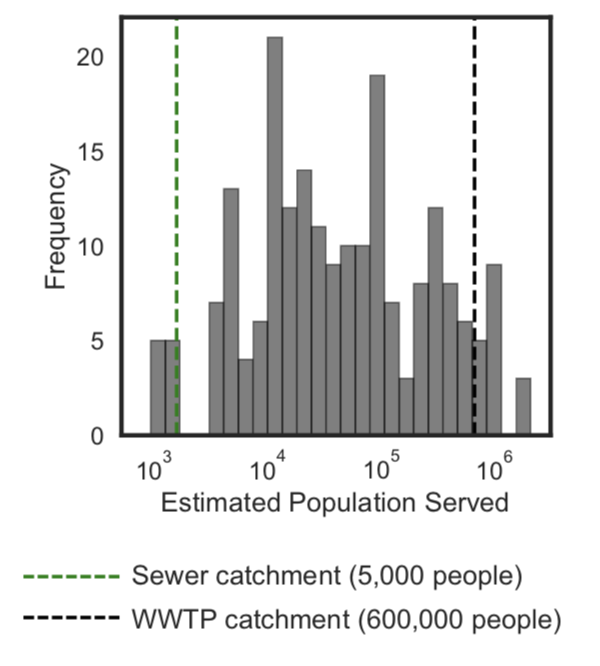
\includegraphics{s1_population_sizes_newton.png}
    \caption{Distribution of catchment sizes in Newton et al, 2015. Green dashed line indicates catchment size of upstream residential manhole and black dashed line indicates estimated catchment size of downstream site sampled in this study.}\label{24hr:figS1}
\end{center}
\end{figure}

\begin{figure}[h]
\begin{center}
    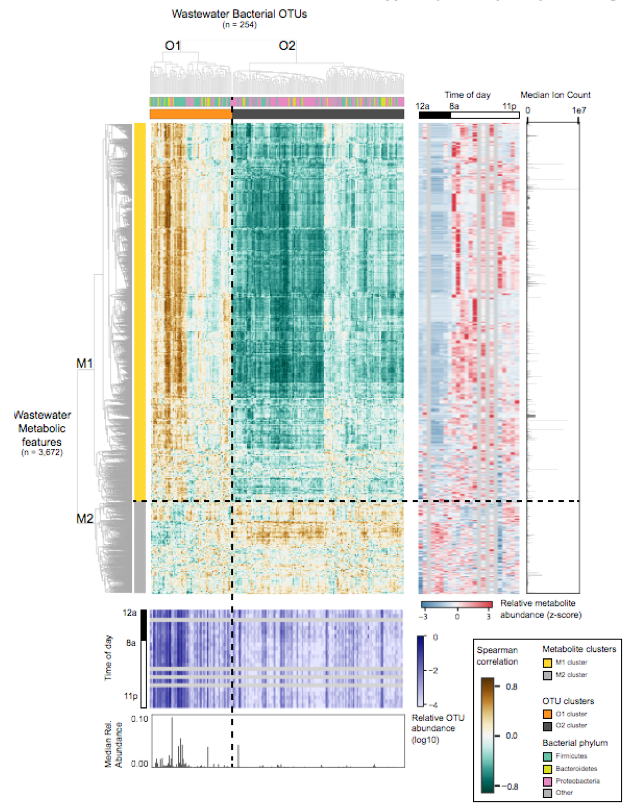
\includegraphics{s2_correlation_heatmaps.png}
    \caption{Co-clustering metabolomics and microbiome data identifies human-associated and environmental clusters. (Middle panel) Spearman correlation between metabolites and OTUs. (Right panel) Z-scored metabolite abundances over 24-hour sampling. Metabolites are in rows, time points are columns. Right-most panel shows daily median ion count of each metabolite feature. (Bottom panel) Heatmap of log10(relative abundance) for each OTU. OTUs are in columns, time points are rows. Bottom-most panel shows daily median relative abundance of each OTU.}\label{24hr:figS2}
\end{center}
\end{figure}

\begin{figure}[h]
\begin{center}
    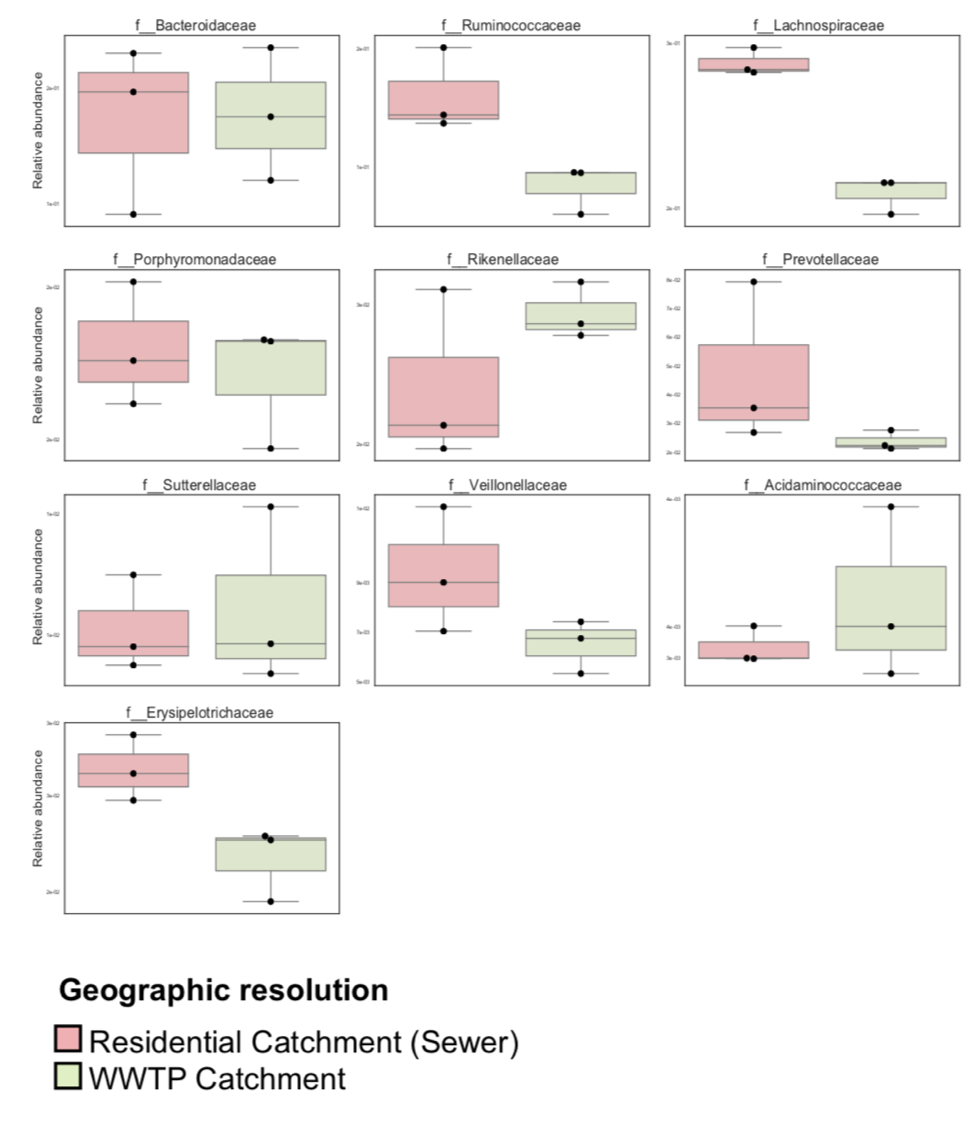
\includegraphics{s3_upstream_downstream_bacteria.png}
    \caption{Abundance of human-associated bacterial families in upstream vs. downstream sample.}\label{24hr:figS3}
\end{center}
\end{figure}

\begin{figure}[h]
\begin{center}
    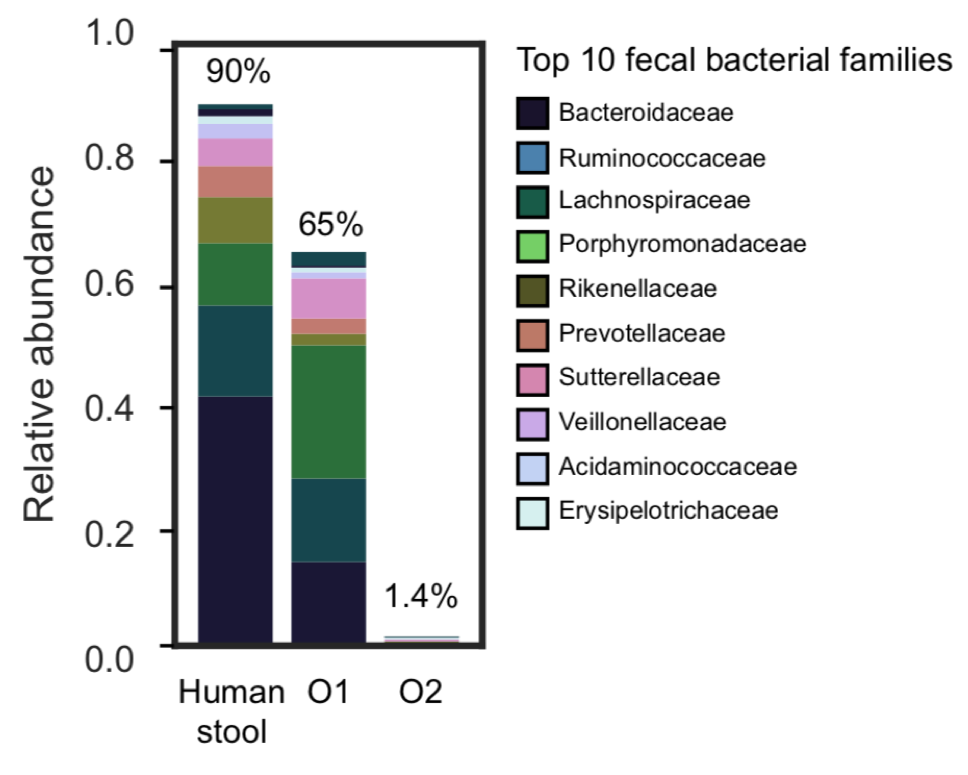
\includegraphics{s4_o1_o2_upstream_downstream.png}
    \caption{Abundance of human-associated bacterial families in OTU clusters O1 and O2.}\label{24hr:figS4}
\end{center}
\end{figure}



% Include the biblio file if you want to have a single, monolithic list of references
% at the end of the thesis. If you do not include the biblio file, you'll have to put
% bibliographies at the end of each chapter.
%\include{biblio}

\end{document}
